% ------------------------------------------------------------------------------
% Este fichero es parte de la plantilla LaTeX para la realización de Proyectos
% Final de Grado, protegido bajo los términos de la licencia GFDL.
% Para más información, la licencia completa viene incluida en el
% fichero fdl-1.3.tex

% Copyright (C) 2012 SPI-FM. Universidad de Cádiz
% ------------------------------------------------------------------------------

\documentclass[a4paper,11pt]{book}

% PAQUETES
\usepackage{./estilo/paquetes}
\usepackage{./estilo/colores}
\usepackage{./estilo/comandos}

% Ruta al directorio de imágenes
\graphicspath{{./img/}} 
 
% METADATOS
\title{OMI: Open Modular Interpreter}
\author{Fco. Javir Bohórquez Ogalla}
\date{Junio 2012} 
 
\begin{document}

\pagestyle{empty}

% PORTADAS
% ------------------------------------------------------------------------------
% Este fichero es parte de la plantilla LaTeX para la realización de Proyectos
% Final de Grado, protegido bajo los términos de la licencia GFDL.
% Para más información, la licencia completa viene incluida en el
% fichero fdl-1.3.tex

% Copyright (C) 2012 SPI-FM. Universidad de Cádiz
% ------------------------------------------------------------------------------


\begin{titlepage}

  \begin{center}

    
\includegraphics[width=0.3 \textwidth]{logo.png} \\
    
    \vspace{2.5cm}
    
    \LARGE{\textbf{ESCUELA SUPERIOR DE INGENIERÍA}} \\
    
    \vspace{1.0cm}
    
    \Large{\textbf{INGENIERÍA TÉCNICA EN INFORMÁTICA DE SISTEMAS}} \\
    
    \vspace{3.0cm}
    
      \begin{center}
   
\includegraphics[scale=2]{logo-doc.png}
   \end{center} 
    
    \vspace{2.5cm}
    
    \Large{Fco. Javier Bohórquez Ogalla} \\
  
    \vspace{0.5cm}

    \large{\today}
    
  \end{center}
\end{titlepage}

\cleardoublepage

% ------------------------------------------------------------------------------
% Este fichero es parte de la plantilla LaTeX para la realización de Proyectos
% Final de Grado, protegido bajo los términos de la licencia GFDL.
% Para más información, la licencia completa viene incluida en el
% fichero fdl-1.3.tex

% Copyright (C) 2012 SPI-FM. Universidad de Cádiz
% ------------------------------------------------------------------------------


\begin{center}

  
\includegraphics[width=0.3\textwidth]{logo.png} \\
  

  \vspace{1.3cm}

  \Large{ESCUELA SUPERIOR DE INGENIERÍA} \\

  \vspace{1.0cm}

  \large{INGENIERÍA TÉCNICA EN INFORMÁTICA DE SISTEMAS} \\

  \vspace{1.3cm}

  \begin{center}
   
\includegraphics[scale=2]{logo-doc.png}
   \end{center} 

  \vspace{1.3cm}

\end{center}

\begin{itemize}
\item \large{Departamento: Ingeniería Informática.}
\item \large{Director del proyecto: Iván Ruiz Rube}
\item \large{Autor del proyecto: Fco. Javier Bohórquez Ogalla}
\end{itemize}

\vspace{0.2cm}

\begin{flushright}
  \large{Cádiz, \today} \\

  \vspace{2.5cm}

  \large{Fdo: Fco. Javier Bohórquez Ogalla}
\end{flushright}

\cleardoublepage

% PRELIMINARES
% ------------------------------------------------------------------------------
% Este fichero es parte de la plantilla LaTeX para la realización de Proyectos
% Final de Grado, protegido bajo los términos de la licencia GFDL.
% Para más información, la licencia completa viene incluida en el
% fichero fdl-1.3.tex

% Copyright (C) 2012 SPI-FM. Universidad de Cádiz
% ------------------------------------------------------------------------------

\thispagestyle{empty}

\noindent \textbf{\begin{Large}\textit{Agradecimientos}\end{Large}} 
\newline
\newline
\noindent\textit{Introduzca aquí, si lo desea, los agradecimientos.}

\newpage

\section {Introducción}
El proyecto OMI comprende una serie de herramientas y recursos que facilitan el aprendizaje de la
teoría de intérpretes y los lenguajes formales, haciendo uso de la interactividad y la documentación.

\subsection{Motivación}
Los cursos académicos relacionados en el estudio de los sistemas intérpretes no cuentan con la ayuda de un caso 
práctico que permita ver una aplicación completa de los conceptos estudiados. Tampoco existe una herramienta interactiva que 
ayude a ver gráficamente cómo funcionan estos sistemas.

\subsection {Alcance}
\subsubsection{Intérprete OMI}
Sistema software capaz de analizar y ejecutar otros programas escritos en un lenguaje específico.

Puede procesar código fuente mediante:
\begin{itemize}
\item La entrada estándar
\item Fichero externo
\item Una consola interactiva (prompt)
\item Puerto TCP
\end{itemize}

 Admite una serie de opciones que modifican el modo en el que se ejecuta, entre las que se pueden destacar:
 \begin{itemize}
 \item Ejecución como servidor.
 \item Ejecución como consola interactiva.
 \item Ejecución detallada. Produce una salida en un formato de datos estándar (JSON), que detalla el proceso 
 llevado a cabo durante la interpretación paso a paso.
\end{itemize}

Puede ser extendido mediante módulos y configurado desde el momento que es construido, lo que permite extender el lenguaje que es interpretado y personalizar
las funciones y características del propio intérprete.

\subsubsection{Lenguaje OMI}
Lenguaje multiparadigma de alto nivel y de propósito general, con tipado dinámico. Su sintaxis pretende ser sencilla y similar a los lenguajes de programación modernos. 
Contempla tipos de datos simples y compuestos, así como un conjunto de operaciones sobre estos. Permite trabajar con variables locales y globales, y procesar estructuras 
y sentencias que permiten controlar el flujo de ejecución tales como if, while, for, inclusión de ficheros, rotura de bloques, parada de la ejecución, saltos a etiquetas, etc.

Permite definir y realizar llamadas a funciones, que pueden hacer uso de parámetros pasados por referencia o valor, y tomar valores por defecto. Además presenta algunas 
características de la programación funcional (clausura de funciones, decoradores, pliegues, aplicación parcial...). 
También permite la definición de clases y la instanciación de estas en objetos, contemplando algunas características de la 
programación orientadas a objetos (métodos mágicos, duck typing, visibilidad, herencia simple...). 

Presenta mecanismos que le dan capacidades reflexivas y que permiten llevar a cabo introspección de tipos. 
Ofrece un conjunto de funciones que permiten operar sobre fechas, procesos y ficheros. 

\subsection{Módulos OMI}
El intérprete OMI puede extender su funcionalidad y características mediante el uso de módulos. El proyecto incluye 
el desarrollo de uno de estos módulos y la documentación del proceso. El módulo gettext añade funciones para la internacionalización de programas.

\subsection{Biblioteca de desarrollo OMI}
Incluye todos los recursos de programación necesarios para construir el intérprete. Está escrita en C++, y se puede incluir en cualquier proyecto software escrito 
en este lenguaje. Aunque forma parte del intérprete, puede ser instalada de forma independiente y usada para el desarrollo de módulos o cualquier otro sistema software 
que necesite interpretar código OMI. 

\subsection{Sitio web del proyecto OMI}
El proyecto OMI incluye un sitio web que sirve como presentación del mismo, además de como medio de acceso a la documentación 
y el software desarrollado. Todas las páginas web pertenecientes al sitio contienen información relativa al proyecto y a las áreas que este
ocupa. Presenta un contenido estático mantenido directamente por el desarrollador. 

\subsection{runTree}
Herramienta online que permite escribir código OMI e interpretarlo. La herramienta describe el árbol sintáctico resultado del análisis del código fuente, y lleva a cabo la ejecución
semántica del mismo paso a paso. Además muestra información de todo el proceso, incluyendo su estado interno y la entrada/salida de datos. 
Esta aplicación representa un cliente del intérprete OMI cuando este es ejecutado como un servidor. Se comunica de forma distribuida con el intérprete y procesa los datos devueltos por el mismo
para mostrarlos al usuario de una forma gráfica y ordenada.   

\section{Estado del arte}
Se exponen los conceptos teóricos necesarios y previos a la construcción del proyecto. Así mismo se lleva a cabo un estudio de las herramientas disponibles en el mercado y se realiza un comparativa a nivel de
funcionalidades y características. 

\section {Planificación}
\subsection{Metodología}
Se ha seguido una metodología iterativa e incremental. Más concretamente se ha tomado como
base el proceso unificado de desarrollo de software, el cual sigue un enfoque dirigido por casos de uso y centrado en 
la arquitectura. El ciclo de vida sigue un enfoque en espiral, dividido en cuatro etapas: determinar objetivos, análisis de riesgos, desarrollo y planificación.
Para la realización de los productos obtenidos en cada paso de la metodología se ha utilizado el lenguaje de modelado UML. 

\subsection{Planificación}
La planificación se divide en una serie de iteraciones. Las etapas y subetapas en las que se divide cada iteración son:

\begin {itemize}
\item Objetivos
\item Riesgos
\item Desarrollo
\begin{itemize}
\item Análisis
\item Diseño
\item Codificación
\item Pruebas
\end{itemize}
\item Planificación
\end {itemize}

La planificación tiene como punto de partida el día 03/11/2014, día en la que se 
comenzó el desarrollo del proyecto. Se ha tomado una jornada laboral de 8 horas, 
y una semana hábil de 5 días. El proyecto recoge los diagramas de Gant correspondiente a la planificación general.

\subsection{Organización}
Para el desarrollo del proyecto se ha usado un equipo de un solo empleado que lleva a cabo los distintos roles implicados. Se ha utilizado 
un único equipo de trabajo con unas prestaciones medias. Además se han utilizado una serie de herramientas software que incluyen sistema operativo, 
generadores de léxicos y gramáticas, compiladores, sistemas de control de versiones, depuradores, servidor web...

\subsection{Costes}
Para los costes relativos a los recursos humanos se ha tomado como referencia un documento BOE publicado el sábado 30 de noviembre de 2013
por el ministerio de empleo y seguridad social. En este documento se recoge la tabla salarial según el convenio colectivo de la empresa 
Trevenque Sistemas de Información SL.

En el desarrollo del proyecto ha participado un único empleado con un salario anual bruto de 18120\euro. El tiempo de desarrollo asciende a 8 meses dando un coste total
en recursos humanos de  12.080,00\euro. Se ha utilizado un único equipo de prestaciones medias con un coste de 409\euro. Las herramientas software utilizadas presentan una licencia
libre y no suponen costes adicional.

\subsection{Riesgos}
Se han identificado los riesgos que pueden originar un efecto negativo en el 
desarrollo del proyecto determinándose la probabilidad de que estos se den y el impacto que tendrían. 
Una vez identificados los riesgos se han definido los planes seguidos para reducir los efectos derivados estos o disminuir
la probabilidad de que ocurran.

El análisis de riesgos se ha llevado a cabo en cada iteración del ciclo de desarrollo. Cada iteración a completado la 
información mostrada. Muchos de los riesgos indicados son comunes a todas las iteraciones realizadas.

Los riesgos se han cuantificado según el impacto que pueden ocasionar y la probabilidad de que se den. Se han organizado según su tipo, quedando divididos 
en: 

\begin{itemize} 
\item Riesgos tecnológicos
\item Riesgos de requisitos
\item Riesgos de soluciones
\item Riesgos de costes, tiempos y recurso
\end{itemize}

\subsection{Aseguramiento de calidad}

Para asegurar una calidad aceptable del producto y los procesos llevados a cabo en el desarrollo se ha tomado como esquema el conjunto de normas ISO 9000. 
Se describen los procesos y actividades seguidas para asegurar la calidad, abarcando todo el desarrollo del proyecto. También se describen los criterios de aceptación
o rechazo de los productos obtenidos en cada fase del desarrollo.

 \section{Requisitos del sistema}
 \subsection{Situación actual}
 Se ha sometido a estudio el proceso de aprendizaje en áreas como la teoría de autómatas, los lenguajes formales y los intérpretes, centrándose en los cursos académicos 
destinados a ello y las limitaciones que estos presentan. Se llega a la conclusión de que los cursos en los que se estudia estas materias implantan la base para entender cómo funcionan y construyen 
estos sistemas, pero no contemplan un caso práctico que aplique estos conceptos de una forma total. Tampoco existen herramientas interactivas que ayuden a ver cómo se 
lleva a cabo el proceso de interpretación.

\subsection{Necesidades}
Se precisa de una herramienta que ayude a ver cómo se implementa y funciona un intérprete para un lenguaje de programación. Se necesita de un soporte que guarde de forma estructurada toda la documentación 
relativa a la construcción de un intérprete. Se precisa de una herramienta interactiva que permita al usuario entender el proceso de interpretación de una forma gráfica y didáctica.

\subsection{Objetivos}
Se llegará a construir un intérprete para un lenguaje de programación con características presentes en la tecnología actual. El proceso quedará correctamente documentado y se pondrá a disposición pública. El intérprete podrá 
ser usado de una forma interactiva y tendrá la capacidad de dar información estructurada del proceso de interpretación. Otros sistemas utilizarán esta información para detallar el proceso de una forma gráfica y flexible.  Se construirá
una aplicación web que aloje toda la documentación generada y desde la cual se pueda hacer uso de herramientas online que se comuniquen con el intérprete. 

\subsection{Requisitos}
Se han descrito los requisitos funcionales del sistema, centrándose en las características del intérprete y el lenguaje subyacente, así como la web y la herramienta online que hace de cliente. Estos requisitos abarcan los modos de ejecución del intérprete y la entrada de datos, los tipos de 
datos, los operadores, estructuras de control, los recursos destinados a satisfacer paradigmas como el orientado a objetos o funcional, las extensiones, la distribución de la documentación, etc. En total se detallan 189 
requisitos funcionales.

Se detallan los requisitos no funcionales que deben cumplir las distintas herramientas desarrolladas tales como el rendimiento (tiempo y espacio), usabilidad, accesibilidad, estabilidad, mantenibilidad y 
la capacidad de concurrencia. 

\section{Análisis del sistema}
\subsection {Modelo conceptual}
Se ha llevado a cabo un análisis de los datos que construyen
el sistema OMI y cómo estos se relacionan. Se describe el 
modelo conceptual de datos del sistema mediante diagramas de clases. Las 
clases son organizadas en paquetes para facilitar la modularidad del sistema
y su entendimiento. 

El proceso de interpretar consiste en tomar código fuente, procesarlo y ejecutar 
su significado semántico. Por tanto el modelo de datos estará constituido por
entidades que guardan un significado concreto y preciso dentro del lenguaje.
Estos elementos, que representan la unidad semántica mínima, 
son denominados nodos ejecutables, debido a que cuando 
son ejecutados producen el resultado semántico asociado.  Muchos nodos ejecutables
por si solos no presentan un resultado semántico completo, por lo que precisan de otros
nodos. 

El diagrama general de paquetes describe los paquetes que componen el 
sistema según el carácter funcional de las entidades que contienen. Un 
paquete podrá contener clases u otros paquetes.

El paquete ``interpreter'' describe las entidades que procesan  
el contenido fuente según el léxico y la gramática del lenguaje OMI. 
El objetivo es generar el árbol de nodos ejecutables correspondiente al
programa. Al procesarse este árbol se aplicará la semántica que encierran 
las líneas de código del contenido fuente, produciéndose de esta forma la ejecución del programa.


El paquete ``runNode'' describe el nodo ejecutable y aquellos tipos de nodos derivados
de este, que son abstractos y que serán extendidos por tipos más específicos.

El paquete ``typeData'' describe los nodos correspondientes a los tipos de datos básicos 
que pueden ser manipulados por el sistema. 

El paquete ``error'' describe el sistema de errores y los nodos ejecutables que permiten
su control.

El paquete ``extensions'' describe el sistema de extensiones del intérprete, el cual
permite extender la funcionalidades del lenguaje de una forma dinámica. Además contiene
el modelado de extensiones concretas.  

Los paquetes siguientes categorizan y agrupan nodos ejecutables según la funcionalidad 
que encierran y el tipo de dato sobre el que operan. 

El último paquete ``rtree'' describe el modelo de datos correspondiente al sistema 
software cliente que hace uso del intérprete de forma online
y representa el estado de este.
 
\subsection {Modelo de casos de uso}
En esta sección se describen los casos de uso que recogen los sistemas que conforman el proyecto OMI, centrándose en el 
sistema intérprete y el cliente runTree.  

El sistema intérprete presenta un actor humano denominado usuario, este puede llevar a cabo casos de uso relativos 
a las distintas formas de entrada de código fuente. Estos casos de uso incluyen un mismo caso denominado ``interpretar'' que describe 
este proceso. El usuario también puede llevar a cabo casos de usos relativos a las distintas opciones del intérprete como ver la ayuda, cagar una extensión, etc.
El sistema intérprete también presenta un actor relativo a un sistema externo que hace uso del mismo cuando este es ejecutado como servidor. El sistema externo,
que hace de cliente, lleva a cabo casos de usos como iniciar una interpretación por red u obtener el paso actual en el proceso de interpretación.

El cliente runTree tiene un único actor denominado usuario, este puede realizar casos de uso relativos al envío de código para su interpretación y la resolución paso a paso del 
proceso. En la ejecución de estos casos de uso el sistema cliente se comunicará con el servidor para llevar a cabo el proceso de interpretación. En el cliente runTree el usuario también podrá llevar 
a cabo casos de usos relativos a la interfaz y la información mostrada, como ver información de nodos, limpiar la salida, ver contenido de la tabla de símbolos, etc. 

\subsection{Modelo de comportamiento}
A partir de los casos de uso se presentan los diagramas de secuencias que modelan los eventos que los sistemas pueden recibir del usuario y los valores de retorno de estos. A partir de los diagramas
de secuencia se obtiene las operaciones que los sistemas presentan, luego se describen los contratos de cada una de las operaciones. 

En general los eventos que reciben el sistema intérprete son los referentes a iniciarlo con una serie de argumentos y de facilitar el contenido fuente a interpretar desde los distintos medios. 
El sistema producirá un valor de retorno correspondiente a la interpretación del código fuente.  También se incluyen los que no se encuentran directamente relacionado con la interpretación como
ver la ayuda o cargar una extensión.

Los eventos que recibe el sistema cliente runTree del usuario son los relativos al envío de código para la interpretación y a la navegación por la descripción paso a paso del proceso.  El sistema retornará la información 
gráfica y textual del estado interno del intérprete en la resolución de cada paso.  También se incluyen diagramas de secuencia relativos a los casos para navegar por la interfaz y operar sobre el contenido fuente.  

En los contratos de operaciones de los sistemas se describe los cambios en la estructura de datos interna de los mismos. En el caso del intérprete toda operación que implique una interpretación de contenido fuente creará 
y relacionará  estructuras de datos como el analizador léxico, el analizador sintáctico, las tablas de símbolos y los nodos ejecutables correspondientes al código procesado. En el caso del cliente las operaciones 
crean estructuras similares debido a que este representa gráficamente el estado interno del intérprete cuando se lleva a cabo la el proceso de interpretación.

\subsection{Modelo de la interfaz de usuario}
Se ha llevado a cabo un análisis de la interfaz de usuario de los distintos sistemas que conforman el proyecto.

El intérprete utilizará una interfaz de consola de comandos. Toda la información de salida la presentará como 
cadenas de caracteres. Así mismo toda la información de entrada la tomará del teclado en formato orden y opciones. 

Por otro lado el cliente runTree presentará una interfaz en la que se disponga de una descripción gráfica de todo el proceso 
de interpretación. Para una descripción del proceso de interpretación se precisa de la visualización del código fuente, un árbol con los nodos
que encierran el significado semántico del código, las distintas tablas de símbolos que referenciarán a variables, funciones y clases, y una consola
en la que se mostrará información textual.

También se presenta un diagrama de navegación en el que se expone las distintas ventanas de la web OMI.

\section{Diseño del Sistema}
\subsection {Arquitectura física}
El intérprete OMI puede funcionar en una arquitectura de escritorio, utilizándose como un comando del sistema operativo. En este caso el comando recibe el código 
fuente a interpretar desde distintos medios. 

Por otro lado el intérprete puede funcionar en una arquitectura cliente/servidor, jugando el rol de servidor. La forma más sencilla es recibiendo el código fuente 
mediante un puerto TCP y procediendo a su interpretación. Sin embargo otro modo de ejecución permite además que el intérprete produzca, a partir de una petición, una salida JSON que detalla el paso actual 
en el proceso de interpretación. De esta forma se puede recorrer paso a paso todo el proceso de interpretación obteniéndose una estructura JSON que defina el estado del intérprete en cada paso.

\subsection{Arquitectura lógica}
\subsubsection{Intérprete}
 El intérprete presenta dos niveles de organización lógica, la capa frontal que procesa la entrada del usuario y el motor que se encarga de producir el resultado semántico correspondiente. 
 
 La capa frontal se compone de un analizador léxico y un analizador sintáctico. El analizador léxico denota un lenguaje regular y se corresponde con un autómata finito. Los estados finales del autómata producen un 
 token que se corresponderá con un elemento léxico del lenguaje como una palabra reservada, un número, un identificador, etc. Los tokens pueden guardar un valor y serán utilizados como entrada por el analizador sintáctico.  
 El analizador sintáctico implementa una gramática libre de contexto de tipo LR(k) , utilizándose así un método de análisis ascendente.  Para construir el analizador sintáctico se utiliza un autómata de pila .  La capa frontal también 
 incluye componentes para capturar la entrada del usuario y facilitar la salida que produce el sistema.

La capa motor está formada por una serie de componentes llamados nodos ejecutables, los cuales encierran un significado semántico concreto. El analizador sintáctico genera un árbol formado por estos nodos. La 
ejecución del árbol producirá el resultado. La ejecución de ciertos nodos generarán de forma dinámica otros nodos que serán referenciados mediante una estructura de datos denominada tabla de símbolos. 

\subsubsection{runTree}
El cliente runTree presenta dos niveles de organización lógica, el front-end se encarga de recibir los datos de entrada del usuario, generalmente código fuente, este es pasado al back-end que se encargará de realizar 
una petición al servidor para que lo procese y devuelva una salida estructurada correspondiente al árbol sintáctico. El back-end procesa esta estructura y el resultado es pasado nuevamente al front-end para que 
sea representado en la interfaz. El usuario podrá realizar acciones para avanzar en el proceso de interpretación, estas acciones serán capturadas por la capa front-end que nuevamente se comunicará con el back-end para 
realizar peticiones al servidor y así obtener la descripción estructurada de cada paso del proceso de interpretación

\subsection{Gramática}
Se define las reglas gramáticales que describen el lenguaje OMI, para ello se hace uso del lenguaje para expresar gramáticas libres de contexto EBNF. También se incluyen diagramas de carril para cada regla. 

\subsection{Comunicaciones}
Se describen las estructuras de datos que el intérprete OMI puede devolver cuando funciona en modo servidor y recibe una petición para iniciar una interpretación de red u obtener el paso actual dentro 
del proceso de interpretación. Se describen las estructuras JSON devueltas haciendo uso de JSON Schema.

\subsection{Diseño de componentes}
Se detalla cómo los distintos objetos interaccionan y se comunican entre sí para
procesar el código fuente introducido por el usuario e interpretarlo, produciéndose así la ejecución del programa codificado. 
Para ello se presenta un diagrama de secuencia para la operación ``interpretar código fuente''. Luego se presentan diagramas de 
comunicación correspondientes a algunas sentencias escritas en el lenguaje.

Para interpretar código fuente el objeto OMI, correspondiente al sistema, creará un analizador sintáctico que codifica las reglas gramaticales. El analizador sintáctico se valdrá de un analizador léxico 
para procesar el código fuente mediante una serie de expresiones regulares que hace corresponder con tokens. El analizador sintáctico utiliza los tokens como entrada para comprobar si se cumple 
alguna regla gramatical. Por cada regla gramatical que se cumpla se creará un determinado nodo ejecutable, produciéndose así un árbol de nodos ejecutables que representa el código fuente.  Este árbol comenzará
a recorrerse en profundidad para ejecutar el significado semántico que encierra cada nodo. 

\subsection{Diseño de la interfaz de usuario}
Se describe el uso del comando ``omi'', correspondiente al intérprete, las opciones y argumentos que admite, y los modos en los que puede ser ejecutado. También se presenta el diseño de la páginas
que conforma cliente runTree y la web del proyecto.

\section{Construcción del sistema}
 Se detallan las herramientas utilizadas en el desarrollo y su versión. También se describe la estructura de ficheros en la que se distribuye el código fuente, y cómo estos se relacionan. Por último se presentan 
 fragmentos de código significativos como la asignación de valores, el uso de variables, o las operaciones básicas.
 
\section{Pruebas del sistema}
La estrategia seguida ha sido que en cada iteración del desarrollo se realicen pruebas relativas a las funcionalidades comprendidas en la misma. Se ha tomado un enfoque de 
caja negra centrada en la especificación de las funciones, la entrada y la salida. Se construyen los casos de pruebas a partir de clases de equivalencia.

Se describe el entorno software y hardware utilizado para las pruebas, que abarca las especificaciones del equipo y las distintas versiones de software utilizado. Las pruebas se realizan desde la perspectiva de
un único rol usuario que realiza programas con el objetivo de probar cada aspecto funcional del sistema.

Las pruebas se han realizado por niveles:

\begin{itemize}
\item Pruebas unitarias: Se llevan a cabo sobre cada artefacto software producido en cada iteración. Estas se centran en cada característica del lenguaje por separado.
\item Pruebas de integración: Incluyen casos de prueba correspondiente a la interacción de varios artefactos. Se centran en el uso conjunto de las características del lenguaje.
\item Prueba funcionales: Tienen como objetivo comprobar la funcionalidad integra del sistema. Se centran en la funcionalidad principal que es interpretar programas completos.  Se incluyen varios 
programas desarrollados en OMI: una calculadora, un sistema de cuestionarios y un programa de IA con el que jugar al tic-tac-toe.
\item Pruebas no funcionales: Se describen pruebas para medir el rendimiento en velocidad y espacio, y la seguridad.
\end{itemize}

\section{Manual de implantación}
Se describen la configuración del entorno hardware y software sobre el que funciona el proyecto OMI, lo que incluye el servidor web, el servidor de dominio, el propio intérprete y la aplicación web. Se detallan 
los requisitos previos para la implantación del sistema, el inventario de componentes y el proceso de instalación llevado. Por último se describen las pruebas de implantación llevadas a cabo.

\section{Manual de usuario}
Se listan las características de los sistemas software desarrollados. Luego se detallan los requisitos previos que se han de cumplir antes la instalación de los mismos. También se describe el uso de los sistemas, lo que incluye:

\begin {itemize}
\item Cómo obtener las herramientas del proyecto.
\item Distintas formas de instalación:
\begin{itemize}
   \item Configuración, compilación e instalación desde código fuente
   \item Instalación de binario precompilado y empaquetado. 
\end{itemize}
 \item Intérprete OMI. Opciones y usos del comando. 
 \item Referencias del lenguaje OMI. Recursos y usos del lenguaje. 
 \item Extensiones del lenguaje. Carga y construcción de módulos.
 \item Funcionamiento cliente/servidor.
 \item Modo que detalla el proceso de interpretación.
 \item runTree. Interfaz y usos del cliente.
\end{itemize}

\section{Conclusiones}
Como se introdujo se ha construido un intérprete modular y completo de un lenguaje de programación de alto nivel, capaz de funcionar de forma distribuida y 
describir mediante estructuras de datos el proceso de interpretación paso a paso. Se ha construido un cliente online que se comunica con el intérprete para 
representar gráficamente el proceso de interpretación. La documentación y las herramientas generadas han sido dispuestas en una web del proyecto. 

Durante el desarrollo del proyecto se han aprendido lecciones y profundizado en el estudio de materias, tales como los intérpretes y lenguajes formales, características 
de los lenguajes de programación actuales, la configuración de sistemas distribuidos, el desarrollo web, etc.

Como trabajo futuro se podría añadir características al lenguaje pertenecientes a los paradigmas contemplados u otros, añadir características al intérprete como la compilación justo a tiempo, 
un mayor detalle en la descripción del proceso de interpretación, etc.

\section{Bibliografía}
Referencias bibliográficas:
\begin{itemize}
\item Compiladores y procesadores del lenguaje (José Antonio Jiménez Millám) [Servicios publicaciones universidad de Cádiz].
\item Compiladores. Principios, técnicas y herramientas 2ªed. (Alfred Aho, Ravi Sethi, Jeffrey Ullman y Monica S. Lam) [Pearson Addison Wesley].
\item El lenguaje unificado de modelado (Booch, Rumbaugh y Jacobson) [Pearson Addison Wesley].
\end{itemize}

Portales webs sobre lenguajes de programación:
\begin{itemize}
\item isocpp.org: Estándar C++.
\item cplusplus.com: C++ referencias y tutoriales.
\item docs.oracle.com: Java Platform, Standard Edition.
\item php.net: PHP documentación y referencias.
\item python.org: Python documentación y referencias.
\item ruby-lang.org: Ruby documentación y referencias.
\item w3schools.com: JavaScript tutoriales y referencias W3C.
\item developer.mozilla.org: JavaScript tutoriales y referencias Mozilla.
\item nodejs.org: Node.js documentación y referencias.
\item uam.es: Manual básico LISP.
\item haskell.org: Haskell documentación y referencias.
\item swi-prolog.org: Prolog documentación y referencias.
\item perl.org: Perl documentación y referencias.
\item scala-lang.org: Scala documentación y referencias.
\end{itemize}
\pagebreak
Otros recursos generales:
\begin{itemize}
\item wikipedia.org
\item stackoverflow.com
\end{itemize}

\section{Licencia}
Todo el software desarrollado se encuentra bajo licencia GPLv3. La documentación generada durante el desarrollo del proyecto se encuentra bajo licencia Creative Commons con libertar para compartir y
adaptar, y prohibiéndose su uso comercial.
% ======================================================================

\newpage


\frontmatter

% INDICES
\tableofcontents
\listoffigures
\listoftables

\mainmatter

% PROLEGÓMENO
\part{Prolegómeno}
\null\vfill
\noindent La primera parte de la memoria del PFC debe contener una introducción y una planificación del proyecto.\\

La introducción es un capítulo que, a modo de resumen, debe contener una breve descripción del contexto de la disciplina en la que el proyecto tiene aplicación y la motivación para su desarrollo, así como del alcance previsto.\\

El segundo capítulo debe incluir una planificación del proyecto. La planificación deberá ajustarse a las prácticas de ingeniería en general, y de la ingeniería del software en particular. Deberá tener en cuenta los plazos, los entregables (documentos y software), los recursos (humanos y de equipamiento inventariable) y el método de ingeniería de software a emplear.
\\

\chapter{Introducción}
% ------------------------------------------------------------------------------
% Este fichero es parte de la plantilla LaTeX para la realización de Proyectos
% Final de Grado, protegido bajo los términos de la licencia GFDL.
% Para más información, la licencia completa viene incluida en el
% fichero fdl-1.3.tex

% Copyright (C) 2012 SPI-FM. Universidad de Cádiz
% ------------------------------------------------------------------------------

El proyecto OMI ofrece un conjunto de herramientas y recursos que ayudan en el aprendizaje 
de la teoría de intérpretes y los lenguajes formales. OMI en si mismo es un intérprete desarrollado 
con la finalidad de servir como caso práctico, aplicando los conceptos estudiados en 
estos campos. Es un intérprete modular, en el sentido de que su funcionalidad y características puede ser extendida mediante módulos.
OMI es código abierto y libre, por lo que puede ser utilizado, estudiado, modificado y/o redistribuido libremente.\\

El nombre OMI también hace referencia al lenguaje que es interpretado. Un lenguaje de programación de alto nivel, de tipado dinámico y de propósito general. Fundamentalmente 
imperativo orientado a objetos, pero que además presenta características propias de otros paradigmas como de la programación funcional. \\

El proyecto OMI pretende facilitar el estudio de los sistemas intérpretes mediante la documentación y la interactividad. Abarcando no solo el diseño y el desarrollo
de uno de estos sistemas, si no el proceso de interpretación en si. De esta forma se presentan herramientas que permiten hacer uso del intérprete a la vez que ilustran
su funcionamiento. 

\section{Motivación}
La teoría de autómatas y los lenguajes formales son la base para la construcción de sistemas intérpretes. Muchos de los conceptos estudiados 
en estos campos sirven para construir otras ramas de estudio como la teoría de intérpretes y compiladores. 

Normalmente, por limitaciones de tiempo, los cursos académicos relacionados con el estudio de estos campos están enfocados a los conceptos teóricos. 
Llevándose a cabo tan solo algunas prácticas que refuerzan el aprendizaje y ayudan a ver la aplicación real mediante casos sencillos y simplificados. 
Sería de gran ayuda en este proceso disponer de un caso práctico completo, que ilustre cómo se define y construye un lenguaje de programación actual, 
y que pueda ser consultado cuándo, dónde y por quién lo desee. OMI pretende ser una fuente de información que complemente el estudio práctico en estas áreas.\\

Aunque existen herramientas que dan soporte a la construcción de sistemas intérpretes, es difícil encontrar alguna que ayude a comprender cómo estos se construyen y funcionan. 
Los intérpretes modernos no están enfocados en ilustrar la tarea que llevan a cabo, tienen como propósito ejecutar programas de forma óptima y efectiva. Sería de utilidad disponer de una 
herramienta que documente los procesos sintácticos y semánticos llevados a cabo durante la interpretación de código fuente. OMI tiene como propósito generar información relativa al proceso 
de interpretación que muestre el funcionamiento del intérprete. 

La comunidad académica no solo precisa de un objeto de estudio, si no también de un objeto que ayude a formar la comunidad. El proyecto OMI pretende ser una base para crear una comunidad 
centrada en el estudio de los lenguajes formales, en las que todos puedan contribuir a la vez de beneficiarse.

\section{Alcance}

El proyecto OMI abarca una serie de herramientas y recursos que ayudan a comprender 
cómo se construye y funciona un sistema intérprete.

\subsection{Intérprete}
El intérprete OMI es la parte fundamental del proyecto, las demás herramientas y recursos se valen o se construyen a partir de este. 
Es un sistema software capaz de analizar y ejecutar otros programas escritos en un lenguaje específico con el mismo nombre.

El intérprete puede procesar código fuente recibido mediante la entrada estándar. También es posible ejecutarlo como una terminal interactiva, mostrando un prompt
e interpretando el código introducido. Por otro lado podrá ser configurado para obtener el código fuente mediante un puerto TCP, funcionando así como un software 
servidor. El software puede recibir una serie de parámetros que serán pasados como argumentos al programa.  Además puede ser ejecutado de forma que produzca una salida en formato JSON relativa a acciones llevadas a cabo durante el proceso.

El intérprete puede ser extendido mediante módulos lo que permite ampliar las posibilidades del lenguaje subyacente. Por otro lado el software 
puede ser configurado desde el momento en el que es construido, de forma que puede prescindir y/o alterar algunas de sus características, adaptándose mejor 
al uso concreto que se le fuera a dar. 

\subsection{Lenguaje} 
OMI es un lenguaje multiparadigma de alto nivel y de propósito general, que presenta un tipado dinámico. Su sintaxis pretende 
ser sencilla y similar a los lenguajes de programación modernos. 
Contempla tipos de datos simples y compuestos, así como un conjunto de operaciones sobre estos. Los tipos de datos que pueden ser 
manipulados por el intérprete OMI comprenden:
\begin{itemize}
  \item Lógicos
  \item Aritméticos
  \item Cadena de caracteres
  \item Array de elementos
  \item Expresiones regulares
  \item Funciones
  \item Referencias
  \item Objetos
\end{itemize}

El intérprete OMI soporta variedad de operadores que trabajan sobre los tipos de datos indicados. Estos son aquellos que se pueden encontrar de forma
nativa en cualquier lenguaje de programación actual, a excepción de los operadores booleanos bit a bit. Esto incluye operadores tales como 
la suma, la potencia, la negación, la concatenación, el ternario, fusión de nulos... Se dispone además de una serie de operadores para la entrada/salida de datos. 

También permite al usuario asignar valores a símbolos variables, que pueden ser utilizados posteriormente en otras expresiones y construcciones del lenguaje. Las 
variables pueden ser locales o globales.

El sistema intérprete es capaz de procesar estructuras de control tales como if, while, switch... Además presenta otras sentencias que operan sobre el flujo de ejecución, 
como por ejemplo la inclusión de ficheros, la rotura de bloques, la continuación de bucle o la parada de la ejecución. También permite la definición de etiquetas y el salto a las mismas.\\

En OMI es posible definir y realizar llamadas a funciones. Estas pueden hacer uso de parámetros por defecto, y estos pueden 
ser pasados por referencia o valor.

OMI es un lenguaje orientado a objetos. Permite la definición de clases y la instanciación de estas en objetos. Contempla algunas características 
propias de este paradigma:
\begin{itemize}
\item Definición de métodos y atributos
\item Método constructor
\item Visibilidad pública y privada
\item Herencia simple
\item Métodos y atributos estáticos
\item Enlace estático en tiempo de ejecución
\item Métodos mágicos
\item Duck typing
\item Tipos de datos básicos como clase de objetos
\end{itemize}

OMI además presenta características propias de la programación funcional:
\begin{itemize}
\item Funciones de primer orden
\item Clausura de funciones
\item Decoradores
\item Pliegues
\item Aplicación parcial
\item Funciones anónimas
\item Listas por compresión
\end{itemize}

OMI es un lenguaje con mecanismos que favorecen la reflexión y permiten llevar a cabo introspección de tipos. 

El lenguaje ofrece una serie de recursos en forma de funciones destinados a la gestión de
ficheros, procesos y fechas.
  
\subsection{Módulos}
OMI puede extender su funcionalidad y características mediante el uso de módulos. El proyecto OMI incluye 
el desarrollo de uno de estos módulos y la documentación de este proceso.

El módulo gettext añade funciones para la internacionalización de programas. Implementa las funciones de la biblioteca de GNU
con el mismo nombre.

\subsection{Biblioteca de desarrollo}
La biblioteca de desarrollo OMI incluye todos los recursos de programación necesarios para construir el intérprete. 
Está escrita en C++, y se puede incluir en cualquier proyecto software escrito en este lenguaje. 
Esta biblioteca puede ser instalada de forma independiente al intérprete, y puede ser usada para el desarrollo de 
módulos o cualquier otro sistema software. Permite construir nodos semánticos a partir de los ya definidos e 
interpretar código fuente escrito en OMI.

\subsection{Sitio web}
El proyecto OMI incluye un sitio web que sirve como presentación del mismo, además de como medio de acceso a la documentación 
y el software desarrollado. Todas las páginas web pertenecientes al sitio contienen información relativa al proyecto y a las áreas que este
ocupa. 
\begin{description}
\item [Página de inicio:] Describe e introduce brevemente el proyecto. Contiene enlaces a las demás secciones del sitio web. Además presenta un
listado de noticias y enlaces de descargas a la última versión del intérprete.
\item [Índice de documentación:] Página que representa un índice de los documentos que conforman el proyecto.
\item [Documentos:] Páginas relativas a la documentación del proyecto en si.
\item [Navegador de clases:] Páginas relativas a la documentación de las clases incluidas en la biblioteca. 
\item [Navegador de ficheros:] Páginas relativas a la documentación de los ficheros que conforman 
el código fuente de la biblioteca y el intérprete.
\item [Navegador de gramática:] Páginas relativas a la documentación gráfica de la gramática del lenguaje.
\item [Descargas:] Página que enlaza la descarga de las distintas versiones del software que conforma el proyecto, disponibles en varios formatos de instalación.
\item [Sobre OMI:] Página con información relativa a la motivación y circunstancias en las que se ha dado el proyecto. Además da detalles sobre los autores y los
organismos implicados en el desarrollo del mismo.
\item [Contacto:] Página con información de contacto.
\end{description}

El sitio web también sirve como enlace a herramientas que permiten hacer uso del intérprete de forma online.

%~ El sitio OMI presenta un di seño adaptativo, por lo que su apariencia se adapta al dispositivo que accede al mismo. 

\subsection{RunTree} 
Herramienta online que permite escribir código OMI e interpretarlo. La herramienta describe el árbol sintáctico resultado del análisis del código fuente, y lleva a cabo la ejecución
semántica del mismo paso a paso. Además muestra información de todo el proceso, incluyendo su estado interno y la entrada/salida de datos. 
Esta aplicación representa un cliente del intérprete OMI cuando este es ejecutado como un servidor. Se comunica de forma distribuida con el intérprete y procesa los datos devueltos por el mismo
para mostrarlos al usuario de una forma gráfica y ordenada.   

\section{Organización del documento}
La documentación recogida en esta memoria presenta el siguiente contenido y organización:

\begin {description}
\item [Planificación:] Se describe la gestión del proyecto. Aspectos tales como la metodología, organización, 
los costes, la planificación, los riesgos y el aseguramiento de la calidad. 
\item [Requisitos del sistema:] Se describe las necesidades y la situación que han originado el desarrollo del proyecto. Además 
se detallan los objetivos y los requisitos que debe cumplir el sistema. 
\item [Análisis del sistema:] Se lleva a cabo el modelado  relativo al análisis del sistema. Haciendo uso de diagramas UML se 
describe el modelo conceptual de datos, el modelo de casos de uso, el modelo de comportamiento y la interfaz de usuario. 
\item [Diseño del sistema:] Aborda la arquitectura lógica y física del sistema, la descripción de la gramática, el diseño de componentes y la
interfaz de usuario.
\item [Construcción del sistema:] En esta sección se describe el entorno de construcción y la organización del código.
\item [Pruebas del sistema:] Se presenta el plan de pruebas seguido, especificando la estrategia seguida, el entorno de pruebas y los distintos
niveles de pruebas realizadas.
\item [Manual de implantación:] Describe cómo se ha de llevar a cabo la implantación de los distintos sistemas software que 
conforman el proyecto para la puesta en producción. 
\item [Manual de usuario:] Representa una guía de referencia para el correcto uso del software.
\item [Conclusiones:] Se detallan los objetivos alcanzados y las lecciones aprendidas en el desarrollo del proyecto.
\item [Bibliografía:] Lista y recapitula la bibliografía empleada en el desarrollo del proyecto.
\item [Información sobre licencia:] Se presenta y detalla información sobre la licencia de uso del software y la documentación.
\end{description}

Por otro lado el conjunto de software desarrollado estará disponible desde varios canales y formatos:
\begin{itemize}
\item CD 
\item Forja de software
\item Apartado de descargas en la web
\end{itemize}
% ======================================================================

   


\chapter{Planificación}
% ------------------------------------------------------------------------------
% Este fichero es parte de la plantilla LaTeX para la realización de Proyectos
En esta sección se trata todos los aspectos relativos a la gestión del proyecto. Se describe el
proceso aplicado para el correcto desarrollo del proyecto, dentro de las limitaciones dadas por 
el alcance, tiempo, calidad y presupuesto.

La gestión del proyecto comprende la implantación de una metodología de desarrollo, viéndose 
esta como la implantación de una serie de pasos, técnicas, procedimientos y demás recursos que
ayuden a desarrollar el producto software dentro de un marco de trabajo. 

Por otro lado también se ha de tratar la planificación del proyecto, quedando este organizado en una 
serie de tareas y actividades derivadas de la metodología implantada. 

En la ejecución de un proyecto es necesario la inversión de una serie de recursos, tales como herramientas, 
personal, equipos, herramientas... Se ha de determinar los recursos asignados a la ejecución del mismo, así como los roles 
de las personas asignadas y la relación entre estas.

El desarrollo de un proyecto software tiene unos costes derivados de los recursos asociados al mismo. Estos recursos
serán tanto materiales como humanos, y tendrán un coste fijo asociado que se utilizará para el cálculo del coste total.

Otra de las tareas que se llevan a cabo durante la gestión de un proyecto software es el análisis de riesgos. Todo proyecto 
esta sujeto a una probabilidad de que se den escenarios de riesgo en los que se pueda ver perjudicada la correcta realización del mismo. 
Se detectarán, listarán y analizarán los riesgos y sus consecuencias, así como la probabilidad de que estos sucedan y las prácticas que se llevarán 
a cabo para mitigar los efectos derivados.

Por último se expondrán las prácticas seguidas para asegurar la calidad del desarrollo y los productos obtenidos en cada paso de la
metodología. Para ello se incluyen los estándares, prácticas y normas aplicados durante el desarrollo. Además 
se recogen los distintos tipos de revisiones, verificaciones y validaciones que se han llevado a cabo, así como los criterios 
para la aceptación o rechazo de cada producto y los procedimientos para implantar acciones correctoras o preventivas.

La planificación expuesta no recoge aspectos como la instalación, el mantenimiento o el soporte. Esta se centra únicamente en el ciclo de desarrollo
del proyecto y no en los procesos posteriores, los cuales, aunque también forman parte del ciclo de vida hábil del software, no se encuentran dentro de 
las etapas de desarrollo del mismo.

\section{Metodología de desarrollo}

Para la realización del proyecto se ha seguido una metodología iterativa e incremental. Más concretamente se ha tomado como
base el proceso unificado de desarrollo de software, el cual sigue un enfoque dirigido por casos de uso y centrado en 
la arquitectura. 

El ciclo de vida sigue un enfoque en espiral, dividido en cuatro etapas: determinar objetivos, análisis de riesgos, desarrollo y planificación.

\begin{description}
\item[Determinar objetivos]: 
   \begin {itemize}
   \item Se fijan los productos a obtener: requisitos, especificación, manuales ...
   \item Se fijan las restricciones a las que estará sujeta el proyecto
   \item Sólo en la primera iteración se lleva a cabo una planificación inicial en esta etapa.
   \end{itemize}
\item[Análisis de riesgos]: 
   \begin {itemize}
   \item Se estudia las posibles amenazas y eventos no deseados, así como los daños y consecuencias derivados de estos.
   \item Se evalúan las distintas alternativas que permitan minimizar los riesgos.
   \end{itemize}
\item[Desarrollo]: 
   \begin {itemize}
   \item Se lleva a cabo el desarrollo de lo fijado en las etapas anteriores.
   \item El desarrollo de cada iteración se divide en cuatro etapas: análisis, diseño, codificación y pruebas.
   \end{itemize}
\item[Planificación]:
   \begin {itemize}
   \item Se analiza los productos obtenidos y el estado del proyecto.
   \item Se lleva a cabo una planificación de la siguiente iteración del ciclo de vida.
   \end{itemize}
\end{description}

En un enfoque en espiral lo más común es que en la primera iteración se ofrezca un prototipo del producto a desarrollar, 
no obstante en el proyecto abordado no ha sido así. En lugar de ello se ha planteado una primera iteración que recoja el alcance 
del proyecto, así como los requisitos y análisis de los riesgos globales, además se realiza una planificación de las iteraciones que seguirán. 
Las demás iteraciones contemplan un subconjunto de estos requisitos, añadiéndose en cada una características al software, y afinando el 
análisis global llevado en la primera y siguientes iteraciones.

Para la realización de los productos obtenidos en cada paso de la metodología se ha utilizado el lenguaje de modelado UML. 
\section{Planificación}

La planificación se divide en una serie de iteraciones. Todas las 
iteraciones con excepción de la primera tienen las mismas etapas
en función de la metodología seguida.

Las etapas y subetapas en las que se divide cada iteración son:

\begin {itemize}
\item Objetivos
\item Riesgos
\item Desarrollo
\begin{itemize}
\item Análisis
\item Diseño
\item Codificación
\item Pruebas
\end{itemize}
\item Planificación
\end {itemize}

La planificación tiene como punto de partida el día 03/11/2014, día en la que se 
comenzó el desarrollo del proyecto. Se ha tomado una jornada laboral de 8 horas, 
y una semana hábil de 5 días.

En cada etapa de la planificación se hacen labores de documentación para que
toda la información relativa al proyecto quede reflejada en la memoria 
del mismo. 

%~ La primera etapa refleja un planteamiento general del proyecto, este se ha ido refinando 
%~ con cada iteración del ciclo de vida. Para ello se han modificado los documentos obtenidos de 
%~ iteraciones anteriores.

\subsection{Diagramas de Gantt de las iteraciones generales}
\FloatBarrier
\begin{center}
\begin{figure}[h]
\centering
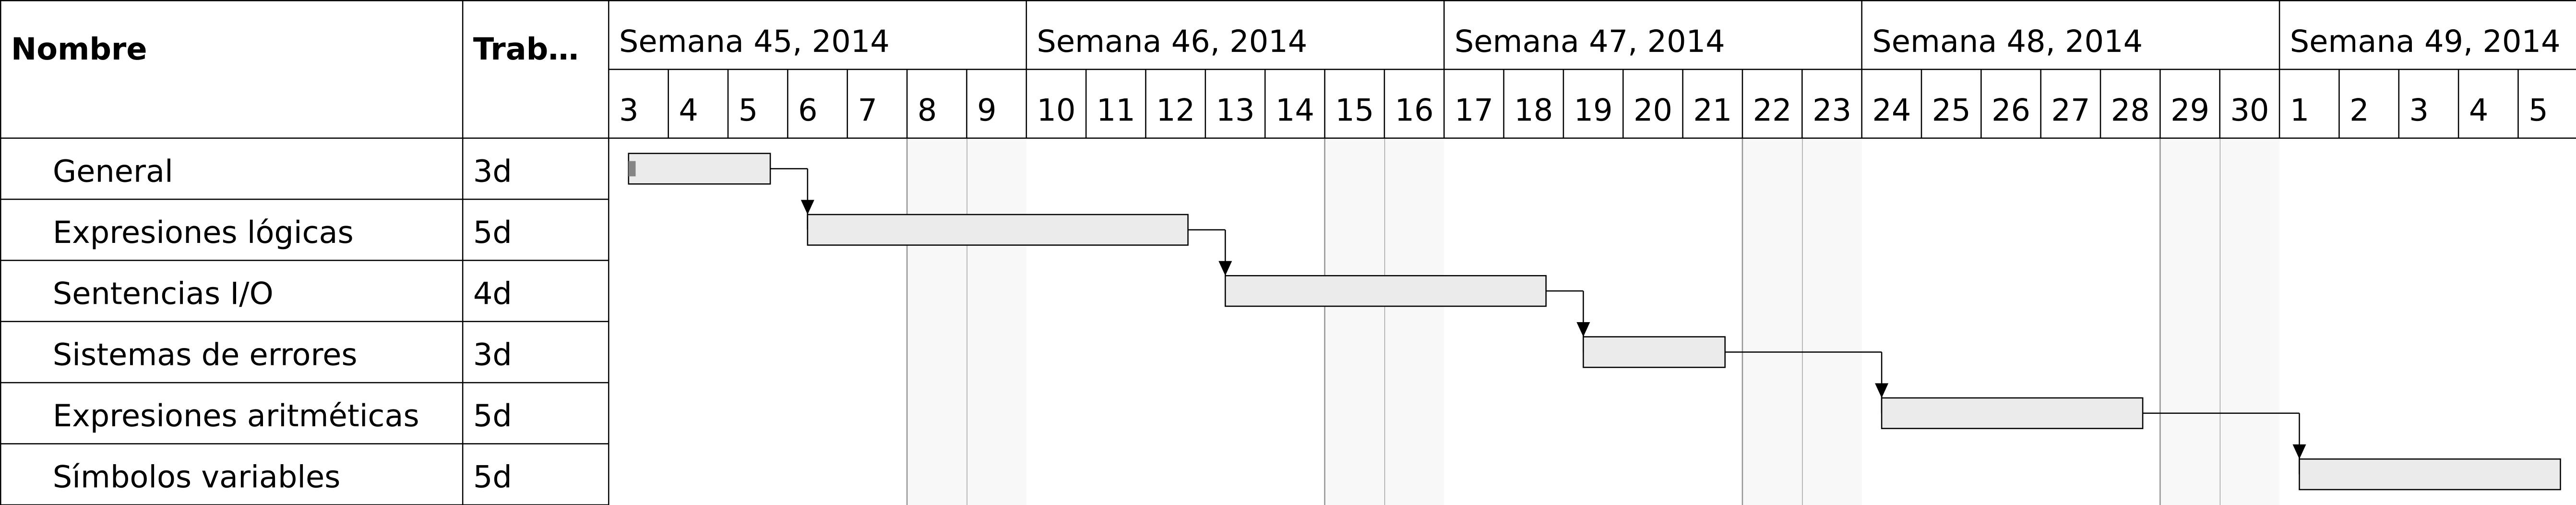
\includegraphics[scale=0.8]{planning/planning_general_1.png} \\
\caption{Planificación general 01 }
\end{figure}
\end{center}
\FloatBarrier

\FloatBarrier
\begin{center}
\begin{figure}[h]
\centering
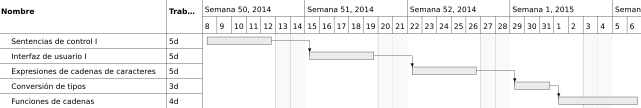
\includegraphics[scale=0.8]{planning/planning_general_2.png} \\
\caption{Planificación general 02 }
\end{figure}
\end{center}
\FloatBarrier

\FloatBarrier
\begin{center}
\begin{figure}[h]
\centering
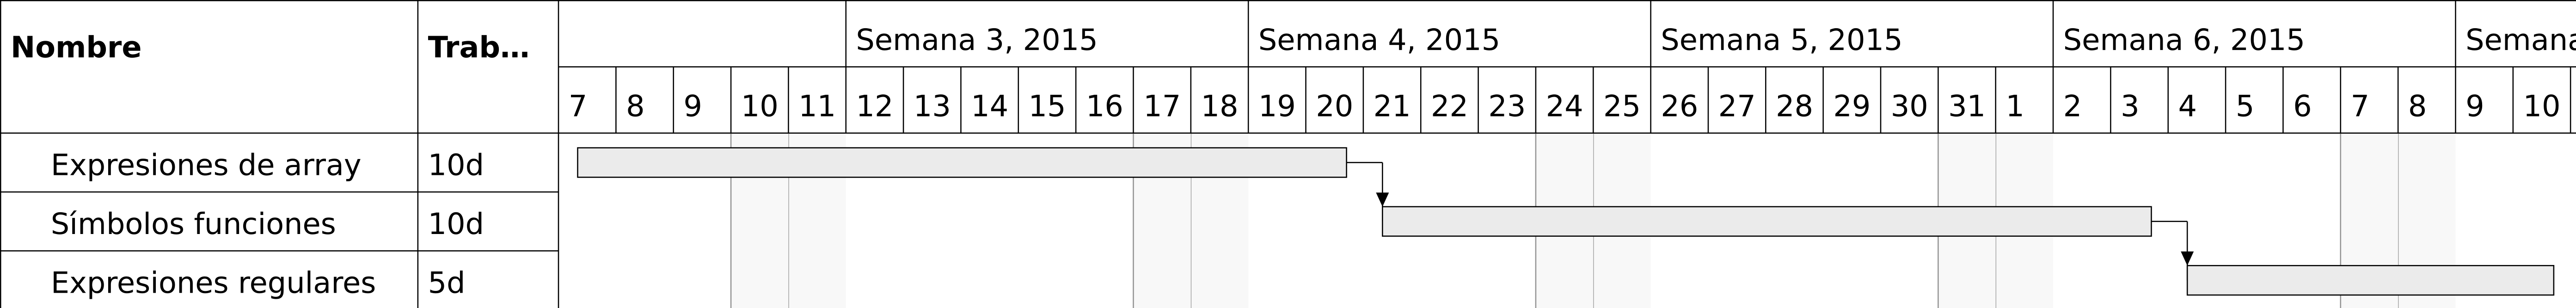
\includegraphics[scale=0.8]{planning/planning_general_3.png} \\
\caption{Planificación general 03 }
\end{figure}
\end{center}
\FloatBarrier

\FloatBarrier
\begin{center}
\begin{figure}[h]
\centering
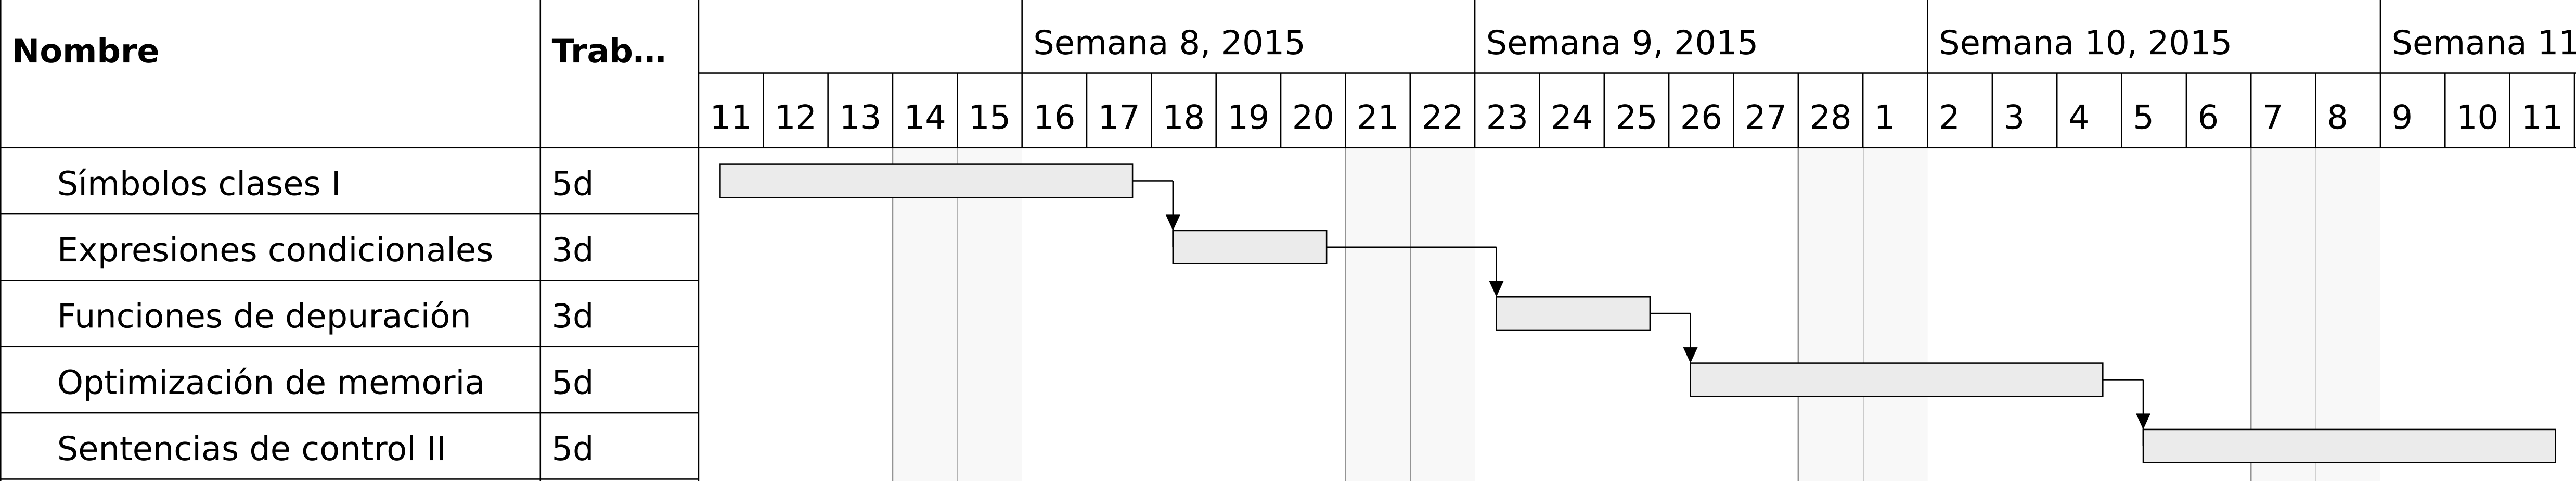
\includegraphics[scale=0.8]{planning/planning_general_4.png} \\
\caption{Planificación general 04 }
\end{figure}
\end{center}
\FloatBarrier

\FloatBarrier
\begin{center}
\begin{figure}[h]
\centering
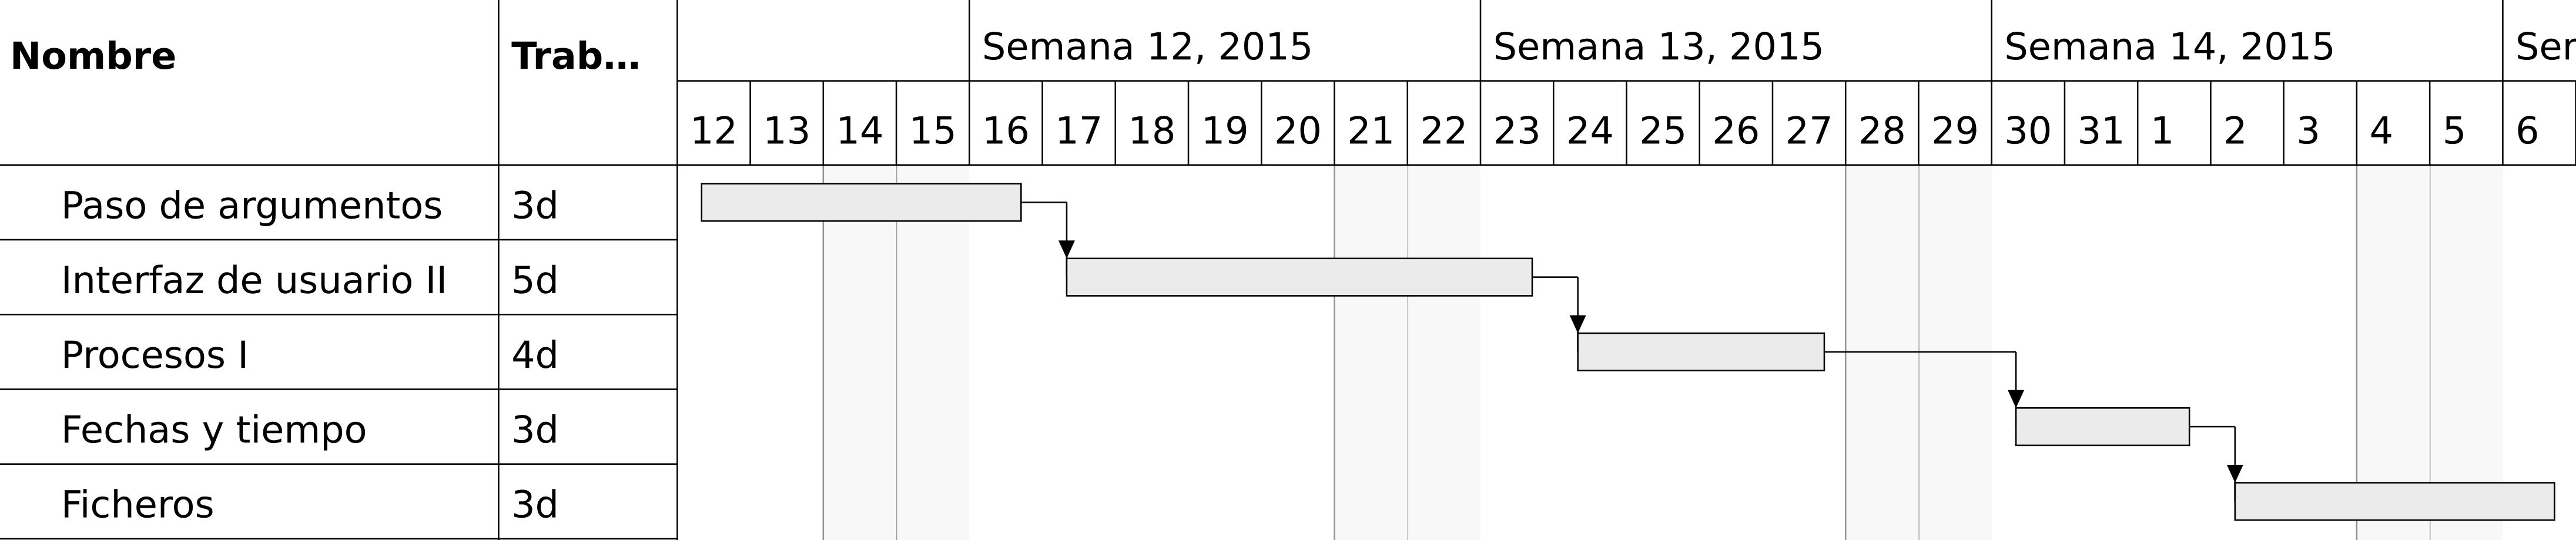
\includegraphics[scale=0.8]{planning/planning_general_5.png} \\
\caption{Planificación general 05 }
\end{figure}
\end{center}
\FloatBarrier

\FloatBarrier
\begin{center}
\begin{figure}[h]
\centering
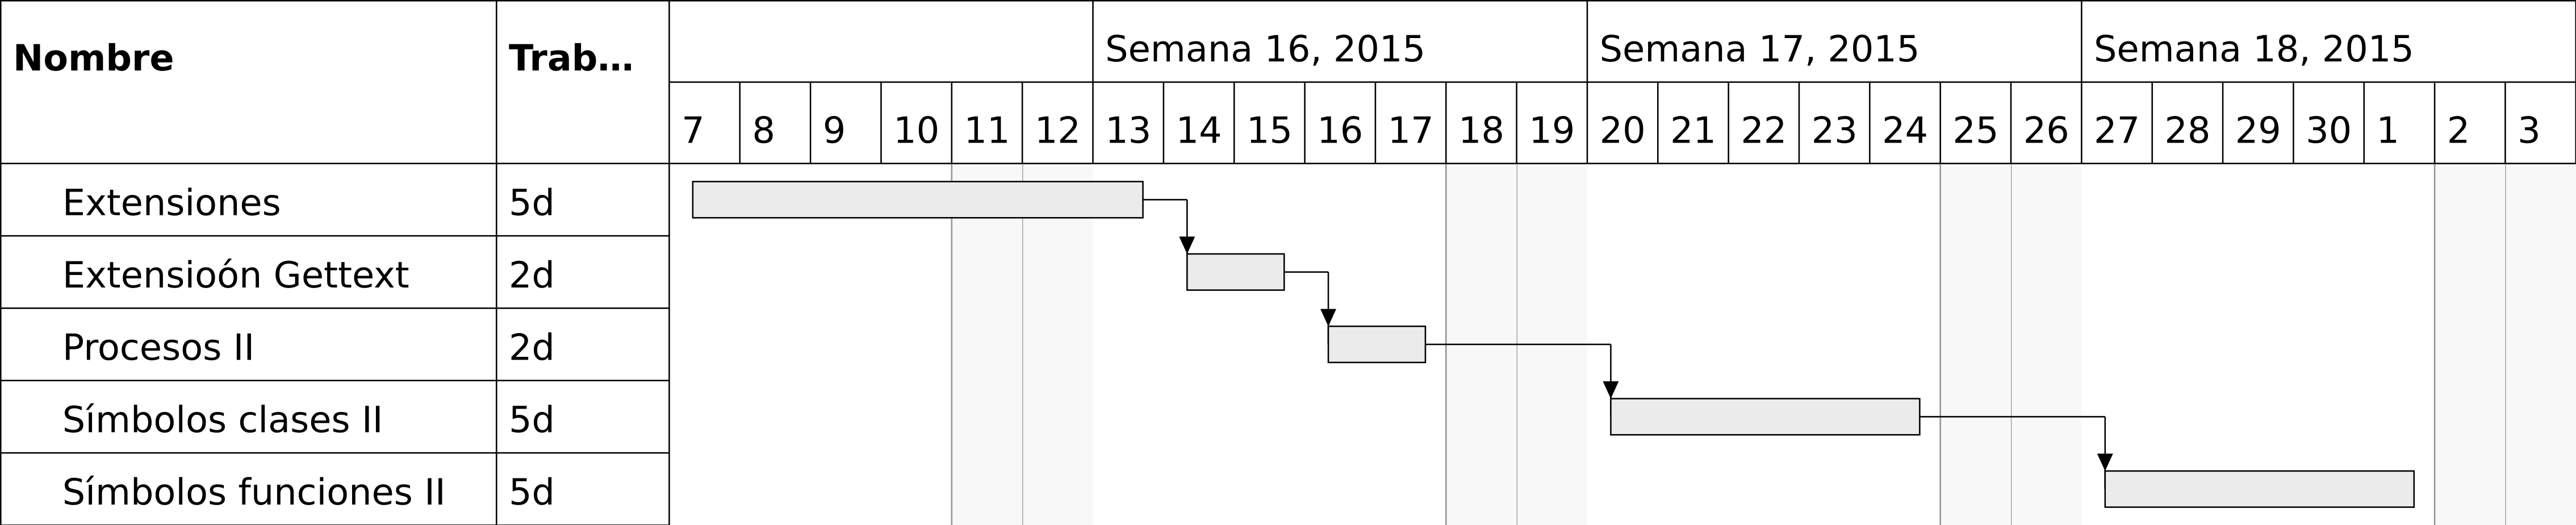
\includegraphics[scale=0.8]{planning/planning_general_6.png} \\
\caption{Planificación general 06 }
\end{figure}
\end{center}
\FloatBarrier

\FloatBarrier
\begin{center}
\begin{figure}[h]
\centering
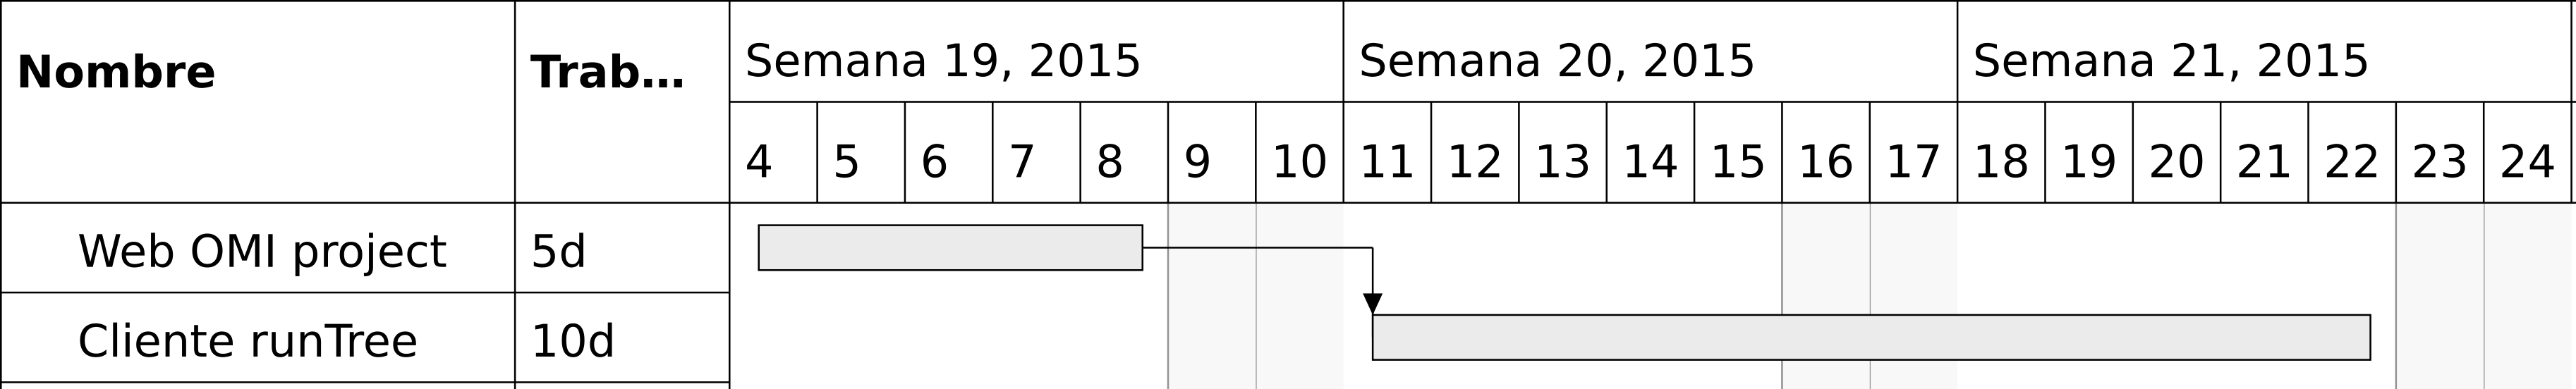
\includegraphics[scale=0.8]{planning/planning_general_7.png} \\
\caption{Planificación general 07 }
\end{figure}
\end{center}
\FloatBarrier

%~ Cada etapa del desarrollo se divide en una serie de tareas y subtareas que se describen a continuación:
%~ 
%~ \begin{description}
%~ \item[Objetivos:] Se define el objetivo y el alcance, y se capturan los requisitos.
%~ \item[Riesgos:] Se analizan los riesgos y se listan las alternativas.
%~ \item[Desarrollo:]  . 
   %~ \begin{description}
   %~ \item[Análisis:] Modelo de casos de usos, conceptual de datos y de comportamiento.
   %~ \item [Diseño:] Gramática, arquitectura y componentes.
   %~ \item [Codificación:] Léxico, sintaxis y semántica
   %~ \item[Pruebas:] Casos de pruebas, pruebas unitarias y verificación.
   %~ \end{description}
%~ \item[Planificación:] Revisión de estado y productos, y planificación de la siguiente iteración
%~ \end{description}

%~ \subsection{General}
%~ \begin{center}
%~ \begin{figure}[h]
%~ \centering
%~ 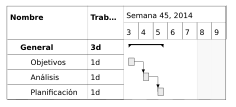
\includegraphics[scale=1]{planning/general.png} \\
%~ \caption{General: 03/11/2014 - 05/11/2014 }
%~ \end{figure}
%~ \end{center}
%~ 
%~ \subsection{Expresiones lógicas}
%~ 
%~ \begin{center}
%~ \begin{figure}[H]
%~ \centering
%~ 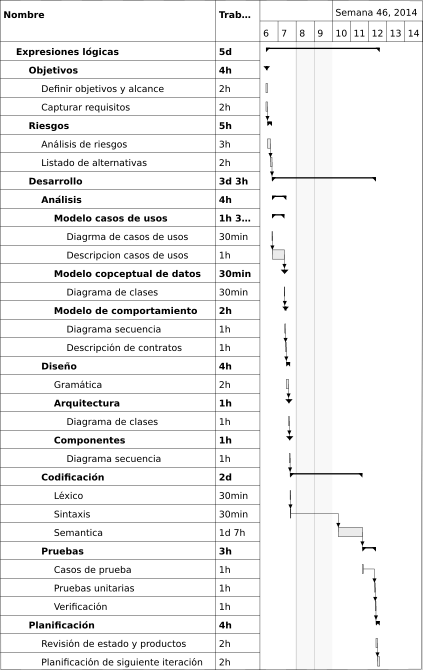
\includegraphics[scale=1]{planning/2-expresiones-logicas.png} \\
%~ \caption{Exp. lógicas: 06/11/2014 - 12/11/2014 }
%~ \end{figure}
%~ \end{center}
%~ 
%~ \subsection{Sentencias de entrada/salida}
%~ 
%~ \begin{center}
%~ \begin{figure}[H]
%~ \centering
%~ 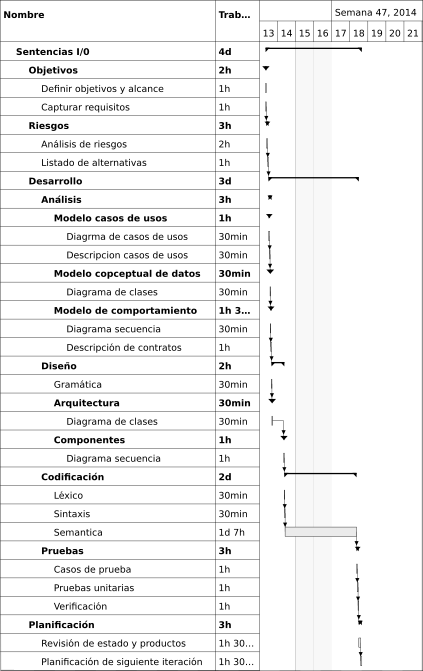
\includegraphics[scale=1]{planning/3-sentencias-io.png} \\
%~ \caption{Sentencias I/O: 13/11/2014 - 18/11/2014 }
%~ \end{figure}
%~ \end{center}
%~ 
%~ \subsection{Sistema de errores}
%~ 
%~ \begin{center}
%~ \begin{figure}[H]
%~ \centering
%~ 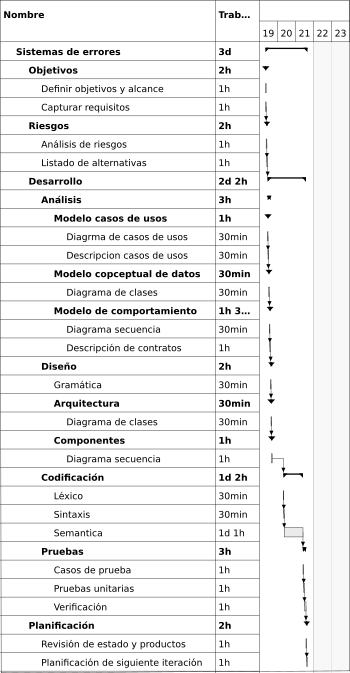
\includegraphics[scale=1]{planning/4-sistema-errores.png} \\
%~ \caption{Sistema de errores: 19/11/2014 - 21/11/2014 }
%~ \end{figure}
%~ \end{center}
%~ 
%~ \subsection{Expresiones aritméticas}
%~ \begin{center}
%~ \begin{figure}[H]
%~ \centering
%~ 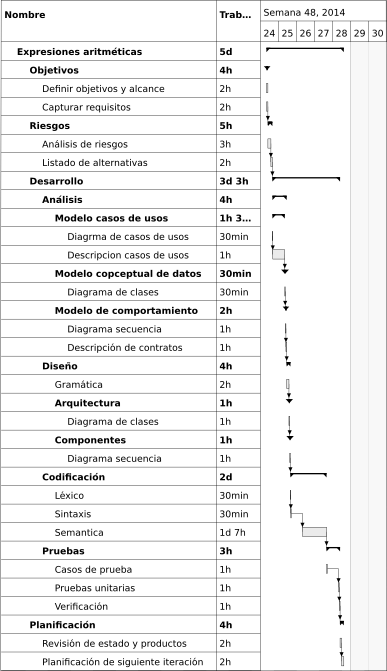
\includegraphics[scale=1]{planning/5-expresiones-aritmeticas.png} \\
%~ \caption{Exp. aritméticas: 24/11/2014 - 28/11/2014 }
%~ \end{figure}
%~ \end{center}
%~ 
%~ \subsection{Símbolos variables}
%~ \begin{center}
%~ \begin{figure}[H]
%~ \centering
%~ 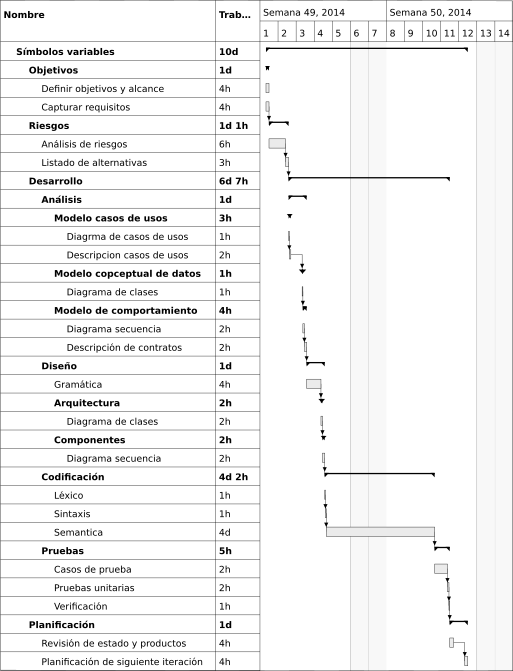
\includegraphics[scale=1]{planning/6-simbolos-variables.png} \\
%~ \caption{Símbolos variables: 01/12/2014 - 14/12/2014 }
%~ \end{figure}
%~ \end{center}
%~ 
%~ 
%~ \subsection{Sentencias de control I}
%~ \begin{center}
%~ \begin{figure}[H]
%~ \centering
%~ 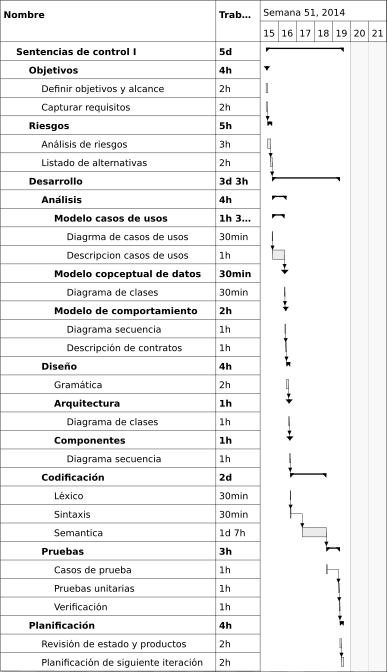
\includegraphics[scale=1]{planning/7-sentencias-control-i.png} \\
%~ \caption{Sentencias control I: 15/12/2014 - 19/12/2014 }
%~ \end{figure}
%~ \end{center}
%~ 
%~ \subsection{Interfaz de usuario I}
%~ \begin{center}
%~ \begin{figure}[H]
%~ \centering
%~ 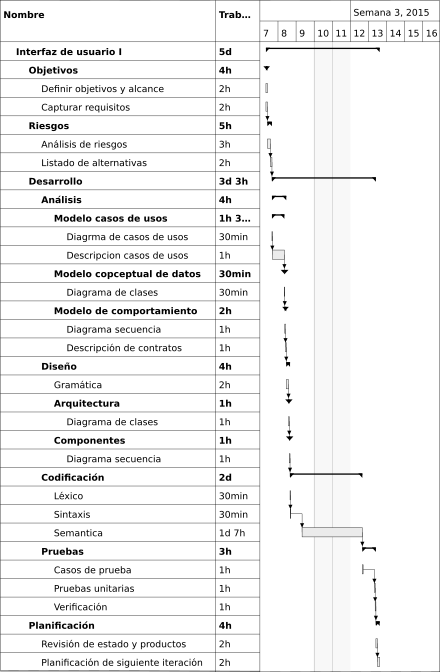
\includegraphics[scale=1]{planning/8-interfaz-usuario-i.png} \\
%~ \caption{Interfaz usuario I: 07/01/2015 - 13/01/2015 }
%~ \end{figure}
%~ \end{center}
%~ 
%~ 
%~ \subsection{Expresiones cadenas de caracteres}
%~ \begin{center}
%~ \begin{figure}[H]
%~ \centering
%~ 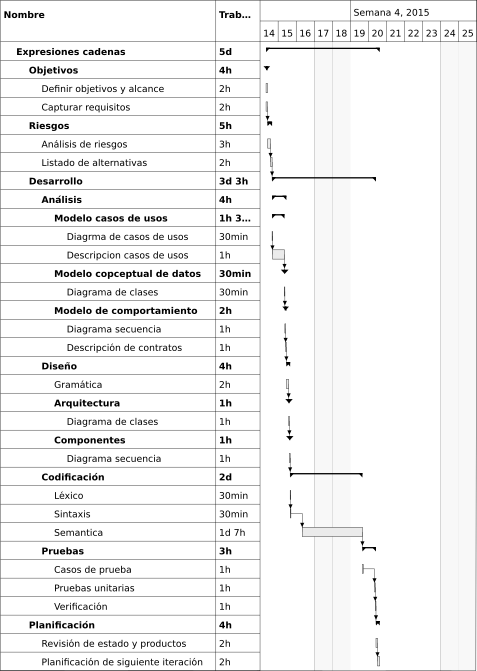
\includegraphics[scale=1]{planning/9-expresiones-cadenas.png} \\
%~ \caption{Interfaz usuario I: 14/01/2015 - 20/01/2015 }
%~ \end{figure}
%~ \end{center}
%~ 
%~ \subsection{Conversión de tipos}
%~ \begin{center}
%~ \begin{figure}[H]
%~ \centering
%~ 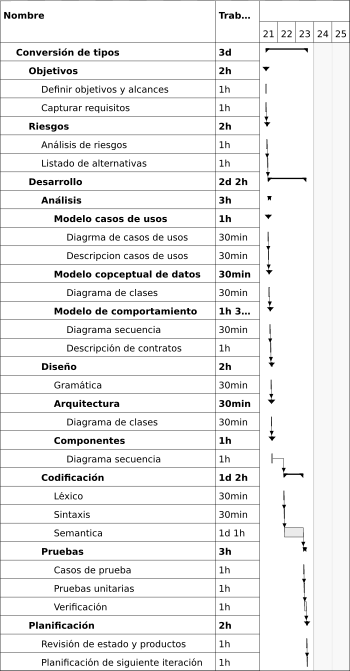
\includegraphics[scale=1]{planning/10-conversion-tipos.png} \\
%~ \caption{Conversión de tipos: 21/01/2015 - 23/01/2015 }
%~ \end{figure}
%~ \end{center}
%~ 
%~ 
%~ \subsection{Funciones de cadenas}
%~ \begin{center}
%~ \begin{figure}[H]
%~ \centering
%~ 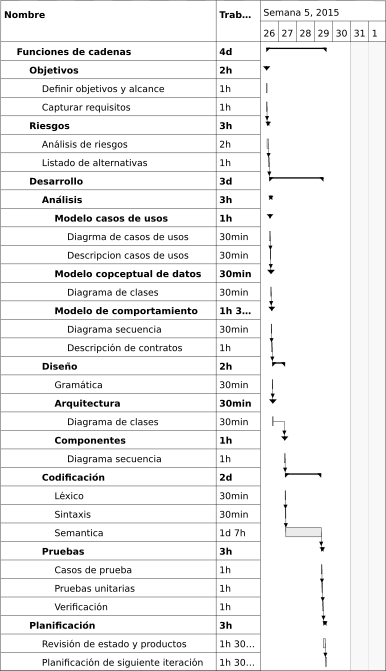
\includegraphics[scale=1]{planning/11-funciones-cadenas.png} \\
%~ \caption{Funciones de cadenas: 26/01/2015 - 29/01/2015 }
%~ \end{figure}
%~ \end{center}
%~ 
%~ \subsection{Expresiones array}
%~ \begin{center}
%~ \begin{figure}[H]
%~ \centering
%~ 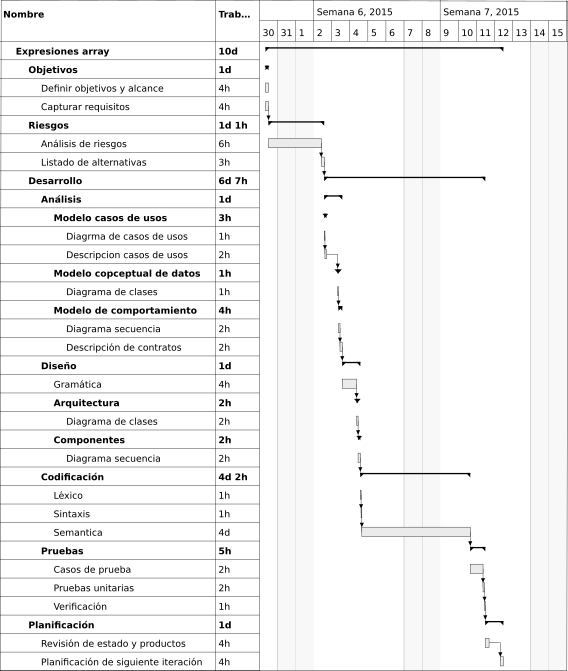
\includegraphics[scale=1]{planning/12-expresiones-array.png} \\
%~ \caption{Expresiones array: 30/01/2015 - 12/02/2015 }
%~ \end{figure}
%~ \end{center}
%~ 
%~ \subsection{Símbolos funciones}
%~ \begin{center}
%~ \begin{figure}[H]
%~ \centering
%~ 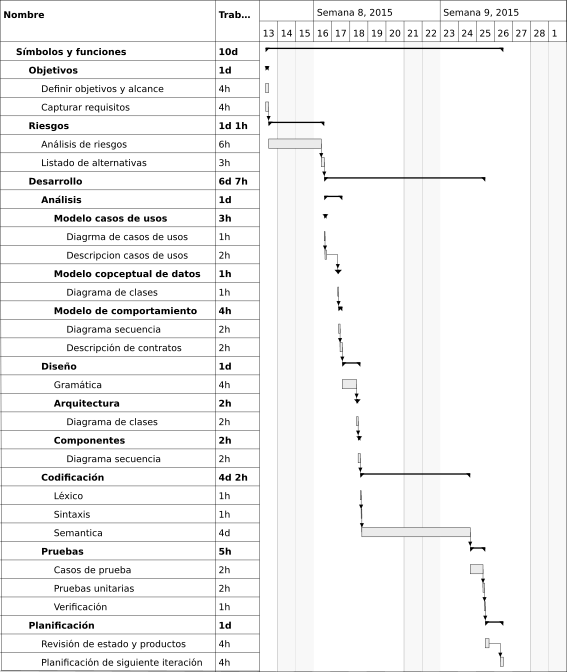
\includegraphics[scale=1]{planning/13-simbolos-funciones.png} \\
%~ \caption{Símbolos funciones: 13/02/2015 - 26/02/2015 }
%~ \end{figure}
%~ \end{center}
%~ 
%~ \subsection{Expresiones regulares}
%~ \begin{center}
%~ \begin{figure}[H]
%~ \centering
%~ 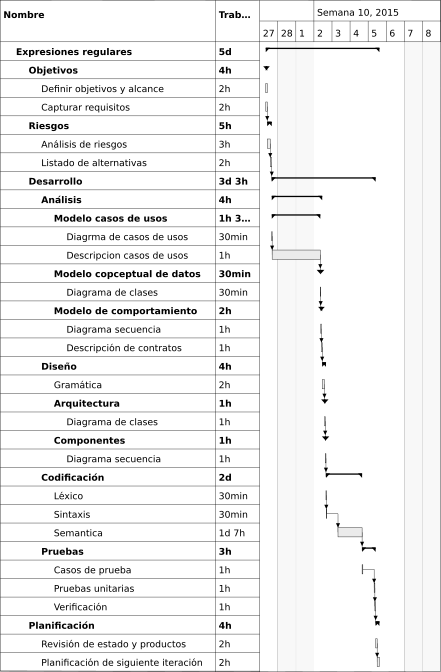
\includegraphics[scale=1]{planning/14-expresiones-regulares.png} \\
%~ \caption{Expresiones regulares: 27/02/2015 - 05/03/2015 }
%~ \end{figure}
%~ \end{center}
%~ 
%~ \subsection{Símbolos clases I}
%~ \begin{center}
%~ \begin{figure}[H]
%~ \centering
%~ 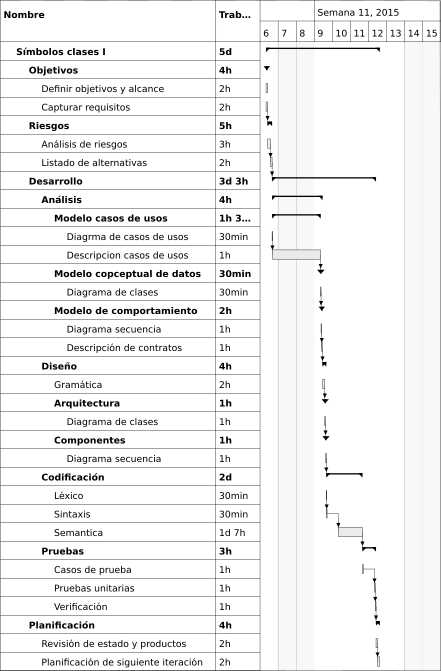
\includegraphics[scale=1]{planning/15-simbolos-clases-i.png} \\
%~ \caption{Símbolos clases I: 06/03/2015 - 12/03/2015 }
%~ \end{figure}
%~ \end{center}
%~ 
%~ 
%~ \subsection{Expresiones condicionales}
%~ \begin{center}
%~ \begin{figure}[H]
%~ \centering
%~ 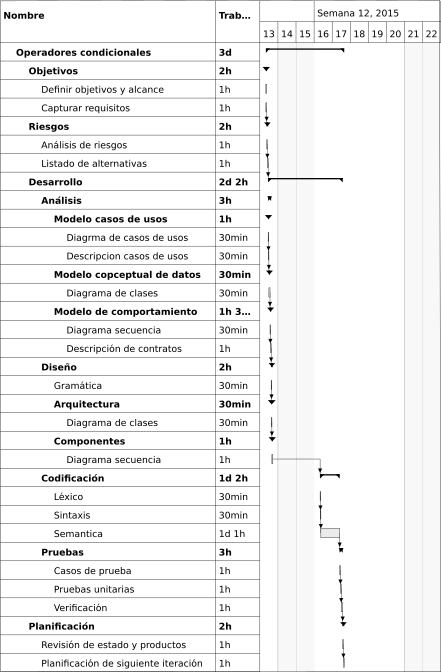
\includegraphics[scale=1]{planning/16-expresiones-condicionales.png} \\
%~ \caption{Expresiones condicionales: 13/03/2015 - 17/03/2015 }
%~ \end{figure}
%~ \end{center}
%~ 
%~ \subsection{Funciones de depuración}
%~ \begin{center}
%~ \begin{figure}[H]
%~ \centering
%~ 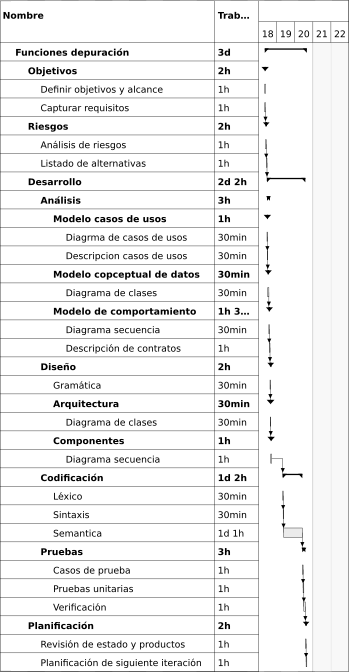
\includegraphics[scale=1]{planning/17-funciones-depuracion.png} \\
%~ \caption{Fúnciones de depuración: 18/03/2015 - 20/03/2015 }
%~ \end{figure}
%~ \end{center}
%~ 
%~ 
%~ \subsection{Optimización de memoria}
%~ \begin{center}
%~ \begin{figure}[H]
%~ \centering
%~ 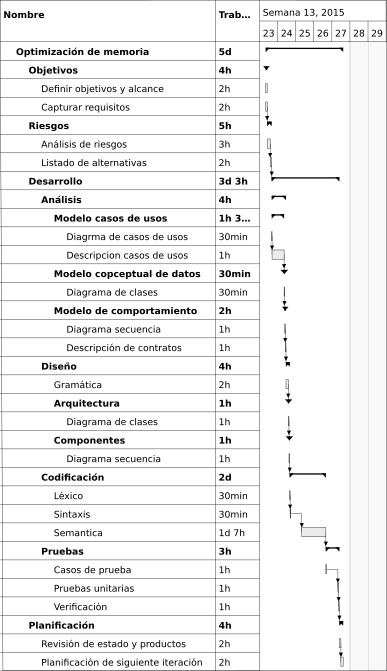
\includegraphics[scale=1]{planning/18-optimizacion-memoria.png} \\
%~ \caption{Optimización de memoria: 23/03/2015 - 27/03/2015 }
%~ \end{figure}
%~ \end{center}
%~ 
%~ \subsection{Sentencias de control II}
%~ \begin{center}
%~ \begin{figure}[H]
%~ \centering
%~ 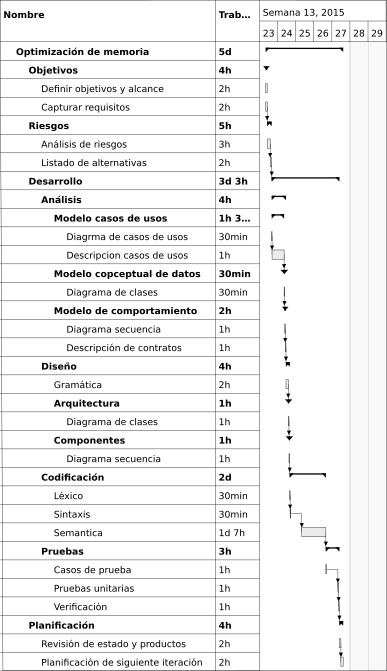
\includegraphics[scale=1]{planning/18-optimizacion-memoria.png} \\
%~ \caption{Optimización de memoria: 23/03/2015 - 27/03/2015 }
%~ \end{figure}
%~ \end{center}
%~ 
%~ 
%~ \subsection{Paso de argumentos}
%~ \begin{center}
%~ \begin{figure}[H]
%~ \centering
%~ 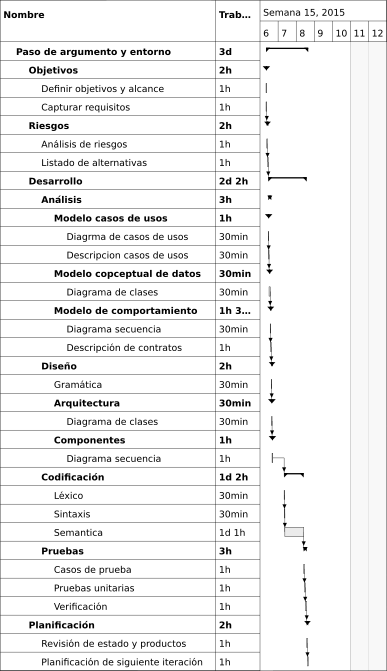
\includegraphics[scale=1]{planning/20-paso-argumentos.png} \\
%~ \caption{Paso de argumentos: 06/04/2015 - 08/04/2015 }
%~ \end{figure}
%~ \end{center}
%~ 
%~ \subsection{Interfaz de usuario II}
%~ \begin{center}
%~ \begin{figure}[H]
%~ \centering
%~ 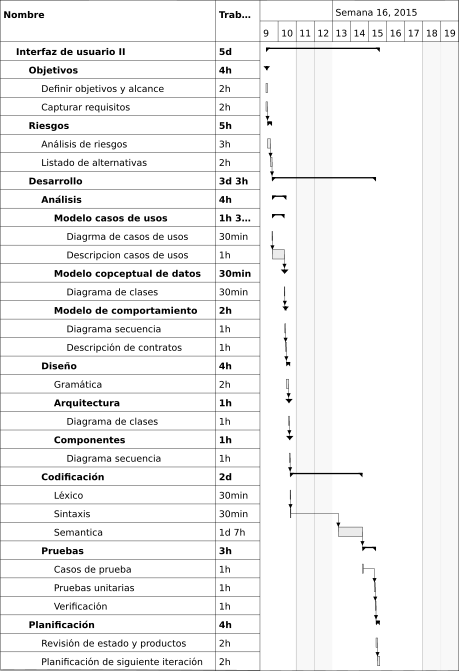
\includegraphics[scale=1]{planning/21-interfaz-usuario-ii.png} \\
%~ \caption{Interfaz de usuario II: 09/04/2015 - 15/04/2015 }
%~ \end{figure}
%~ \end{center}
%~ 
%~ \subsection{Procesos I}
%~ \begin{center}
%~ \begin{figure}[H]
%~ \centering
%~ 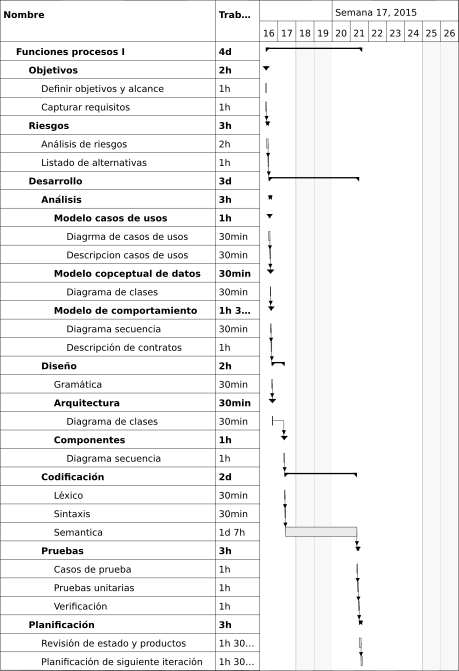
\includegraphics[scale=1]{planning/22-funciones-procesos-i.png} \\
%~ \caption{Procesos I: 16/04/2015 - 21/04/2015 }
%~ \end{figure}
%~ \end{center}
%~ 
%~ \subsection{Fechas y tiempo}
%~ \begin{center}
%~ \begin{figure}[H]
%~ \centering
%~ 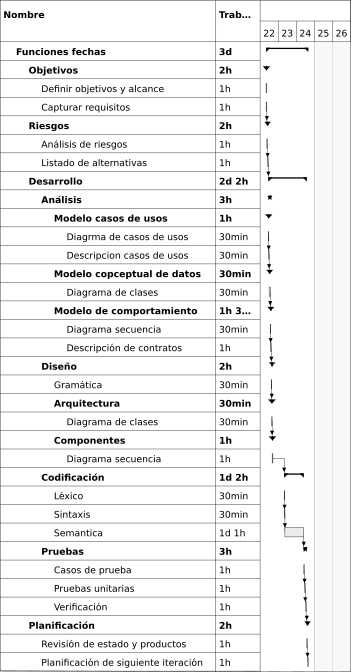
\includegraphics[scale=1]{planning/23-funciones-fechas.png} \\
%~ \caption{Fechas y tiempo: 22/04/2015 - 24/04/2015 }
%~ \end{figure}
%~ \end{center}
%~ 
%~ \subsection{Ficheros}
%~ \begin{center}
%~ \begin{figure}[H]
%~ \centering
%~ 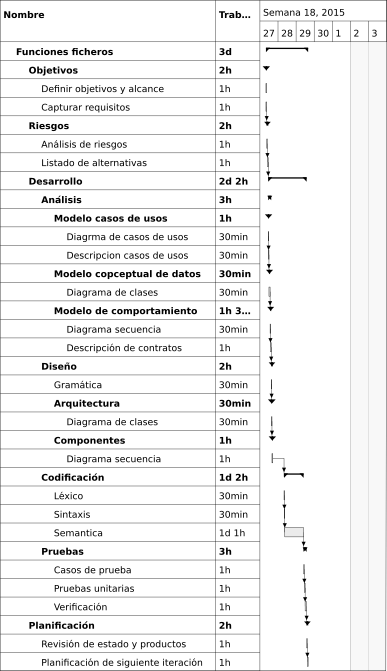
\includegraphics[scale=1]{planning/24-funciones-ficheros.png} \\
%~ \caption{Ficheros: 27/04/2015 - 29/04/2015 }
%~ \end{figure}
%~ \end{center}
%~ 
%~ \subsection{Extensiones}
%~ \begin{center}
%~ \begin{figure}[H]
%~ \centering
%~ 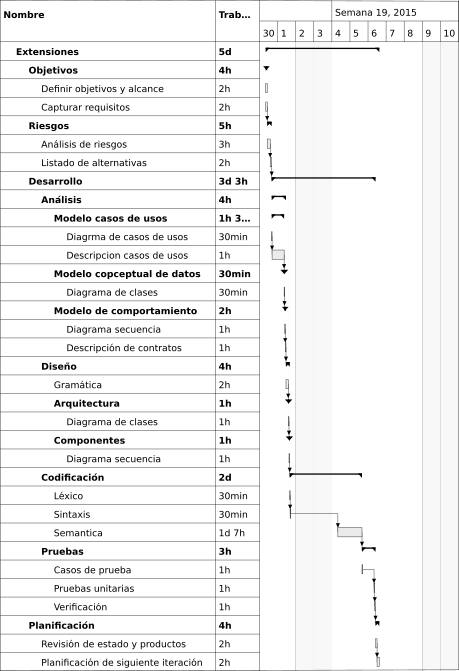
\includegraphics[scale=1]{planning/25-extensiones.png} \\
%~ \caption{Extensiones: 30/04/2015 - 06/05/2015 }
%~ \end{figure}
%~ \end{center}
%~ 
%~ \subsection{Extensión gettext}
%~ \begin{center}
%~ \begin{figure}[H]
%~ \centering
%~ 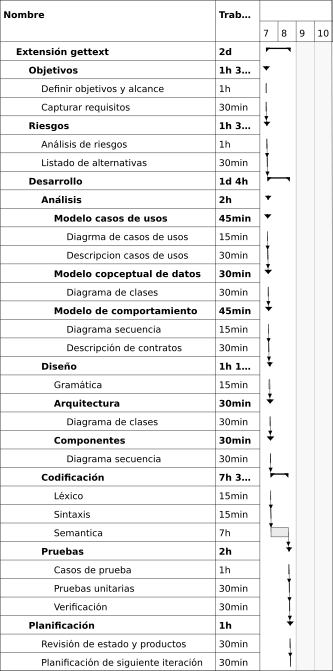
\includegraphics[scale=1]{planning/26-extension-gettext.png} \\
%~ \caption{Extensiones gettext: 07/05/2015 - 08/05/2015 }
%~ \end{figure}
%~ \end{center}
%~ 
%~ 
%~ \subsection{Procesos II}
%~ \begin{center}
%~ \begin{figure}[H]
%~ \centering
%~ 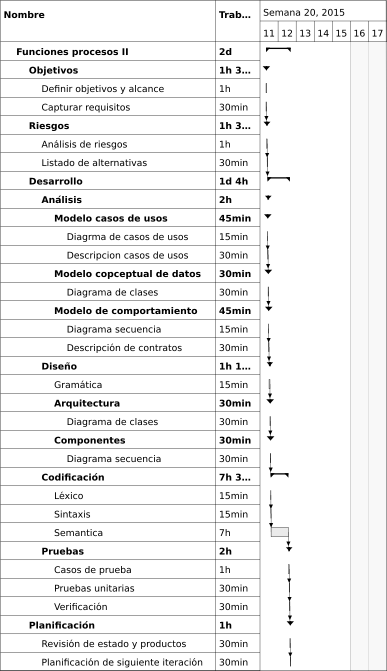
\includegraphics[scale=1]{planning/27-funciones-procesos-ii.png} \\
%~ \caption{Procesos II: 11/05/2015 - 12/05/2015 }
%~ \end{figure}
%~ \end{center}
%~ 
%~ \subsection{Símbolos clases II}
%~ \begin{center}
%~ \begin{figure}[H]
%~ \centering
%~ 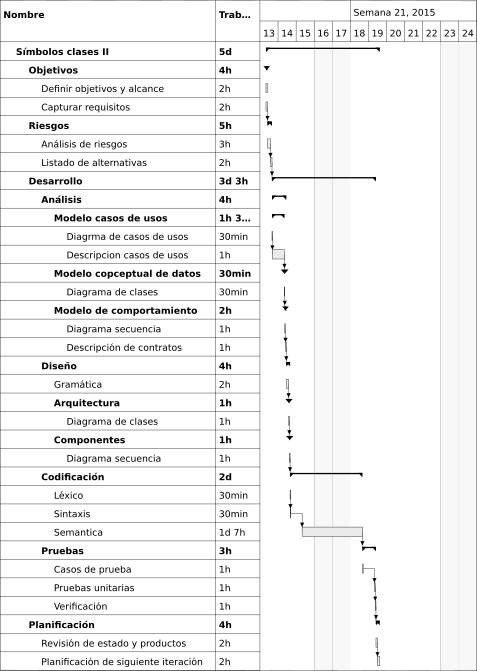
\includegraphics[scale=1]{planning/28-simbolos-clases-ii.png} \\
%~ \caption{Símbolos clases II: 13/05/2015 - 19/05/2015 }
%~ \end{figure}
%~ \end{center}
%~ 
%~ 
%~ \subsection{Símbolos funciones II}
%~ \begin{center}
%~ \begin{figure}[H]
%~ \centering
%~ 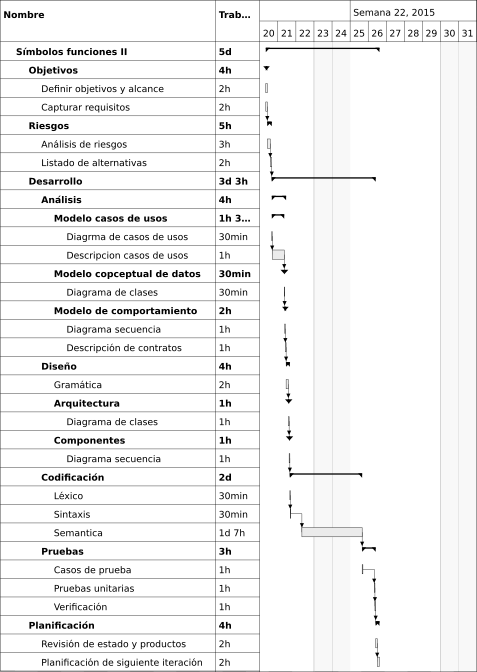
\includegraphics[scale=1]{planning/29-simbolos-funciones-ii.png} \\
%~ \caption{Símbolos funciones II: 20/05/2015 - 26/05/2015 }
%~ \end{figure}
%~ \end{center}


\section{Organización}
Para la realización del proyecto se ha utilizado los siguientes recursos humanos :
\begin{description}
%~ \item[Iván Ruiz Rube:] Director de proyecto, control de calidad. 
\item[Fco. Bohórquez Ogalla:] Director de proyecto, analista, diseñador de arquitectura, diseñador de sistemas, desarrollador, tester, control de calidad
\end{description}

Además se han utilizado los siguientes recursos materiales:
\begin{description}
\item [Equipo de trabajo 1:] Computadora para las tareas de gestión, administración, desarrollo y documentación. 
%~ \item [Equipo de trabajo 2:] Computadora para las tareas de desarrollo y documentación
\end{description}

Las herramientas utilizas son las siguientes:
\begin{description}
\item [Sistema operativo:] GNU/Linux. 
\item [Entorno integrado de desarrollo:] Geany.
\item [Generador léxico:] Flex.
\item [Generador sintáctico:] Bison.
\item [Compilador:] GCC.
\item [Depurador:] GDB.
\item [Herramientas para la construcción automática:] Autoconf, automake, make.
\item [Desarrollo de diagramas:] Dia, railroad diagram generator.
\item [Control de versiones:] Subversion.
\item [Creación de documentación:] Latex, Doxygen.
\item [Planificación:] Planner.
\item [Bibliotecas de desarrollo:] readline, boost. 
\item [Servidor HTTP: ] Apache.
\item [Intérprete de Scripts de servidor:] PHP.
\item [Navegador web:] Firefox, Chrome, Explorer.
\item [Conversor latex a HTML:] latex2html.
\item [Editor gráfico:] Gimp, Inkscape.
\item [Comunicación:] Servicio gratuito de correo electrónico. 
\end{description}

\section{Costes}
A continuación se presenta el coste relativo a los recursos humanos invertidos en el desarrollo del 
proyecto. Para ello se ha tomado como referencia el documento BOE publicado el sábado 30 de noviembre de 2013
por el ministerio de empleo y seguridad social. En este documento se recoge la tabla salarial según
el convenio colectivo de la empresa Trevenque Sistemas de Información SL.
\begin{table}[h]
\begin{tabular}{|l|l|l|l|} \hline
\textbf{Empleado} & \textbf{Grupo} & \textbf{Salario anual bruto} & \textbf{Salario mensual bruto}  \\ \hline
%~ Iván Ruiz Rube & Directivo técnico & 26.652,92\euro & 2.221,07\euro  \\ \hline
Fco. Bohórquez Ogalla & Programado senior & 18.120,00\euro & 1.510,00\euro \\ \hline
\end{tabular}
\caption{Salarios}
\end{table}


El tiempo de desarrollo asciende a 8 meses a tiempo completo. El coste de los recursos humanos puede ser consultado en la tabla \ref{table:totalcost}.
\begin{table}[h]
\begin{tabular}{|l|l|} \hline
%~ \textbf{Iván Ruiz Rube} &  17.768,56\euro \\ \hline
\textbf{Fco. Bohórquez Ogalla } &  12.080,00\euro \\ \hline
\textbf{Total} &  12.080,00\euro \\ \hline
\end{tabular}
\caption{Costes totales}
\label{table:totalcost}
\end{table}
 
 Para el desarrollo del proyecto se ha necesitado de un equipo con una potencia y prestaciones medias. El
 coste de los recursos materiales que suponen estas computadores puede consultarse en la tabla \ref {table:hardcost}.
 
 \begin{table}[h]
 \begin{tabular}{|l|l|l|} \hline
\textbf{Computador \tiny{i5-4460/ 4GB/ 1TB} } & 1x & 409,00\euro \\ \hline
\textbf{Total} & & 409,00\euro \\ \hline
\end{tabular}
\caption{Equipos}
\label{table:hardcost}
\end{table}

Las herramientas utilizadas en el desarrollo del proyecto tiene licencia libre. El uso de estas herramientas no
suponen coste adicional para el desarrollo del proyecto. 

\section{Riesgos}

En este punto se listan los riesgos identificados. Estos pueden originar un efecto negativo en el 
desarrollo del proyecto. Además se muestra la probabilidad de que estos se den y el impacto que tendrían. 
Una vez identificados los riesgos se definen los planes seguidos para reducir los efectos derivados estos o disminuir
la probabilidad de que ocurran.

El análisis de riesgos se ha llevado a cabo en cada iteración del ciclo de desarrollo. Cada iteración a completado la 
información mostrada. Muchos de los riesgos indicados son comunes a todas las iteraciones realizadas. 

Los riesgos analizados según el impacto que pueden ocasionar en el proyecto quedan divididos en:
\begin {description}
\item[Insignificantes:] No merecen ser tenidos en cuenta.
\item[Tolerables:] Están dentro de un margen de aceptación, por tanto no comprometen el proyecto, ni el producto, ni la organización.
\item[Graves:] Comprometen gravemente el proyecto, el producto o la organización.
\item[Críticos:] Amenaza la supervivencia del proyecto, el producto o la organización.
\end{description}

Para dar claridad al análisis, la probabilidad de que se dé un determinado escenario de riesgo se presenta de forma relativa como sigue:
\begin{description}
\item[Muy baja:] $<10\%$.
\item[Baja:] del $10$ al $25\%$.
\item[Moderada:] del $25$ al $50\%$.
\item[Alta:] del $50$ al $75\%$.
\item[Muy alta:] $>75\%$.
\end{description}

Los riesgos quedan organizados en distintas categorías para un mejor análisis.

%~ Riesgos tecnológicos: derivados del software y hardware utilizados.
%~ Riesgos personales: asociados a las personas involucradas en el desarrollo.
%~ Riesgos organizacionales: relacionados a la organización.
%~ Riesgos de herramientas: resultantes de las herramientas de software utilizadas.
%~ Riesgos de requerimientos: surgen de los cambios en los requerimientos.
%~ Riesgos de estimación: proceden de las estimaciones de costes y recursos. \\

\subsection{Riesgos tecnológicos}
Son los riesgos derivados del software y hardware necesarios para el desarrollo del 
proyecto.\\

\begin{table}[h]
\begin{tabular}{|l|c|c|} \hline
\textbf{Riesgo} & \textbf{Probabilidad} & \textbf{Impacto} \\ \hline
Los recursos no están disponibles a tiempo & Baja & Tolerable \\ \hline
\shortstack[l]{\\Fallos en el sistema operativo \\u otros software de sistema}  & Baja & Tolerable \\ \hline
Fallos en el hardware de desarrollo & Baja & Grave \\ \hline
Errores de configuración & Baja & Tolerable \\ \hline
\shortstack[l]{\\Actualización del sistema\\no realizada correctamente} & Baja & Tolerable \\ \hline
Integridad y privacidad de los datos & Baja & Grave \\ \hline
Manipulación deliberada de los programa & Moderada & Grave \\ \hline
\shortstack[l]{\\Las herramientas de comunicación \\ no se encuentran disponibles} & Baja & Insignificante \\ \hline
\shortstack[l]{\\El repositorio de código no se encuentra \\ disponible} & Baja & Tolerable \\ \hline
\end{tabular}\hfill\\
\caption{Riesgos tecnológicos}
\end{table}

En el caso de que los recursos materiales, hardware de desarrollo, no estén disponibles a tiempo se puede comenzar con tareas de definición y 
análisis. Si la demora se hace demasiado extensa se cancelará el pedido del hardware y se realizará a otro proveedor. Esto puede ocasionar
un retraso de días que puede ser mitigado dedicando este tiempo a tareas en las que no se precise de hardware. 

Si se produce algún fallo en el software de sistema que da soporte al desarrollo este puede derivar en pérdidas de datos. La solución sería gestionar la incidencia
o reinstalar el sistema. La perdida de datos se puede mitigar si se realizan copias de seguridad periódicas. Como medida preventiva se pueden guardar puntos de restauración del sistema
para prevenir o mitigar la demora de tiempo que esto podría ocasionar.

Es posible que se produzcan fallos en el hardware sobre el cual se desarrolla el proyecto, esto puede ocasionar retrasos de entregas o la perdida de los datos. 
Para prevenir y mitigar este efecto negativo se puede realizar copias periódicas de los datos y mantener los equipos en un estado de funcionamiento óptimo, bien refrigerados 
y sin exposición a agentes externos. 

Si se produce algún error en la configuración del sistema es posible que algunas características de este dejen de funcionar, en muchos casos esto puede llegar a ser perjudicial para 
el proyecto. Para prevenir y mitigar este efecto se deberán realizar copias de seguridad, además se deberá minimizar la cantidad de software instalado en los equipos. En el caso de producirse un 
fallo de configuración del sistema que afecte directamente a la ejecución del proyecto se deberá invertir tiempo para corregir las causas y administrar el sistema.

En algunos casos una actualización del sistema que da soporte a la ejecución del proyecto puede ocasionar fallos en el mismo o en la configuración. Para ello además de 
las soluciones y prácticas comentadas en los puntos anteriores, se puede minimizar el número de actualizaciones que no sean críticas o que no sean indispensables para 
el desarrollo del proyecto. Como medida de actuación el sistema deberá ser restablecido mediante un administrador cualificado. 

La integridad y privacidad de los datos se puede ver comprometida por algún uso indebido de los mismos o por agentes ajenos al proyecto. Para prevenir y mitigar los efectos de este escenario 
se realizarán copias de seguridad  periódicas y se hará uso de un software de control de versiones. Además se protegerá el acceso a los datos mediante técnicas como claves de acceso, configuraciones de red pocos permisivas
(por ejemplo mediante el uso de firewalls), configuraciones óptimas del sistema (en cuanto servicios y programas), cifrado, no permitir la conexión de dispositivos extraibles, etc. Es muy importante en este punto 
controlar además los permisos de publicación, transferencia y portabilidad que tienen los empleados sobre los datos, quedando registrada y validada toda operación de esta naturaleza. Como medida de
actuación ante un escenario de este tipo los datos quedarán en cuarentena y se llevará a acabo un análisis forense que determine los agentes implicados y los motivos.

Es posible que en algunos casos los programas que conforman el sistema sobre el que se desarrolla sean manipulado de forma consciente o inconsciente por una persona integrante del equipo o ajena 
al mismo. Para prevenir este escenario se acotará el uso del equipo al propósito que este tiene, no se permitirá la instalación de software adicional, se protegerá el acceso al sistema mediante claves robustas y se 
usará software antivirus. Como medida de actuación se bloqueará el acceso al proyecto a cualquier software que se tenga constancia de que se encuentre manipulado o infectado por alguna clase del 
malware, y el equipo implicado se podrá en cuarentena para evaluar el impacto de lo ocurrido.  

Las herramientas de comunicación son un elemento clave en el desarrollo de un proyecto. Depender de terceros para dar soporte al proyecto en este aspecto puede llegar a ser perjudicial. Para 
prevenir pérdidas en el servicio se puede usar clientes estables, fiables y consolidados en el mercado. Para mitigar la perdida de información que supondría una caída del servicio se puede hacer
copias de toda la información enviada por estos medios. Como medida de actuación, siempre y cuando sea necesario una comunicación, se utilizarán otros medios de comunicación como el teléfono. 

El repositorio en el cual se aloja el código fuente puede sufrir caídas en el servicio. Para mitigar y prevenir este tipo de incidencias se alojará el sistema de control de versiones en alguna
máquina de la infraestructura local al proyecto. Esto bloquea o dificulta el acceso remoto al código, lo cual tiene sus ventajas ya que disminuye el grado de exposición, pero hace que el acceso 
al código esté condicionado por un equipo local, siendo de vital importancia la disponibilidad y visibilidad de este. 

%~ \subsection{Riesgos personales}
%~ En esta sección quedan registrados los riesgos asociados a las personas involucradas en el proyecto. 
%~ 
%~ \begin{tabular}{|l|c|c|} \hline
%~ \textbf{Riesgo} & \textbf{Probabilidad} & \textbf{Impacto} \\ \hline
%~ Cambios en el personal directivo & Baja & Crítico \\ \hline
%~ Cambios en el personal ejecutivo & Baja & Grave \\ \hline
%~ \end{tabular}\hfill\\\\
%~ 
%~ Los cambios en el equipo directivo de un proyecto pueden amenazar drásticamente la supervivencia y desarrollo de este. 
%~ El nuevo personal no tiene porque compartir los mismos criterios que el anterior, y lo normal es que no conozca aspectos
%~ internos del mismo. Un cambio directivo en el proyecto puede ocasionar replanteamientos de cuestiones que ya se encontraban cerradas.
%~ Este tipo de riesgos es difícil de prevenir por otros medios que no sean contratos laborales, y aún así no se podría asegurar que el equipo se mantendrá. 
%~ Para mitigar el efecto que un cambio de este tipo podría ocasionar toda decisión directiva deberá quedar analizada, argumentada y registrada. 
%~ 
%~ El personal ejecutivo es esencial para el desarrollo de un proyecto, por lo que un cambio de este tipo en el equipo puede suponer un alto riesgo 
%~ para el desarrollo. Al igual que en el punto anterior los contratos laborales pueden prevenir en cierto grado el riesgo. Para mitigar el efecto se 
%~ deberá documentar todo los procesos y productos obtenidos. Como medida de actuación, siempre que sea posible, el anterior personal podría instruir al
%~ nuevo hasta que tome la destreza y conocimientos suficientes.
%~ 
%~ \subsection{Riesgos organizativos}
%~ 
%~ En esta sección se presentan y analizan los riesgos relativos a la organización del proyecto. 
%~ 
%~ \begin{tabular}{|l|c|c|} \hline
%~ \textbf{Riesgo} & \textbf{Probabilidad} & \textbf{Impacto} \\ \hline
%~ Las tareas no quedan bien definidas y/o acotadas & Moderada & Tolerable \\ \hline
%~ Las tareas no quedan bien distribuidas & Moderada & Tolerable \\ \hline
%~ No se atribuyen responsabilidades & Baja & Tolerable \\ \hline
%~ No se establece una jerarquía de prioridades & Baja & Tolerable \\ \hline
%~ La comunicación entre el equipo no es suficiente & Moderada & Tolerable \\ \hline
%~ \end{tabular}\hfill\\
%~ 
%~ Si las tareas no quedan bien definidas y acotadas se originará fallos en la comunicación y el entendimiento entre
%~ los integrantes del equipo, pudiendo en muchos casos originar trabajo extra y la consecuente dilatación en los tiempos. 
%~ Para prevenir y mitigar este efecto se deberá realizar una descripción minuciosa y detallada de las mismas, utilizando un lenguaje 
%~ sencillo y directo. El plan de actuación ante estas situaciones será la aclaración de los puntos que fueron confusos, mientras que la parte 
%~ que no llegó a entender las cuestiones planteadas no deberá presuponer nada y pedirá la aclaración pertinente. 
%~ 
%~ Si las tareas no se encuentran bien distribuidas puede darse exceso de trabajo por algunas de las partes, ocasionando efectos de parada en el 
%~ proceso de desarrollo. Por otro lado otros recursos pueden quedar ociosos. Para evitar y mitigar este escenario se deberá analizar y planificar todo 
%~ el trabajo a realizar. En el caso de que una planificación incorrecta derive en problemas de este tipo se deberá replantear el trabajo.
%~ 
%~ Un equipo en el que las responsabilidades no queden bien atribuidas puede originar en la falta de implicación y corrección por alguna de 
%~ las partes. Para prevenir y mitigar este efecto se deberá hacer una correcta planificación, involucrando al personal y haciéndoles entender la importancia de su trabajo. 
%~ 
%~ Si no se establece una jerarquía de prioridades en las tareas puede ocasionar la perdida de tiempo en tareas menos importantes, mientras que otras más prioritarias y de las que
%~ existan dependencias quedarán paradas. 
%~ Para evitar esto se deberá realizar una planificación y hacer entender a todo el equipo las prioridades marcadas. Bajo esta circunstancias se deberá retribuir prioridades 
%~ y hacer que todo el equipo sea consciente de estas.
%~ 
%~ Si no se mantiene una comunicación suficiente el proyecto puede verse perjudicado en su ejecución. El equipo directivo puede no conocer el estado verdadero del proyecto 
%~ y las decisiones tomadas no contar con toda la información posible. Para mitigar y prevenir este escenario se pueden realizar reuniones constantes. Como medida de actuación ante 
%~ esta situación se deberá comunicar a los implicados la importancia de la información que poseen.

\subsection{Riesgos de requisitos}

Son riesgos que surgen de los requisitos, ya sean debido a que estos han cambiado o que no se han recogido correctamente.
\begin{table}[h]
\begin{tabular}{|l|c|c|} \hline
\textbf{Riesgo} & \textbf{Probabilidad} & \textbf{Impacto} \\ \hline
Especificación de requisitos insuficiente & Moderada & Grave \\ \hline
Captura de requisitos errónea & Moderada & Grave \\ \hline
Casos de uso complejos o mal redactados & Baja & Tolerable \\ \hline
\shortstack[l]{\\No se han capturado todos los datos\\ que definen o con los que trabaja el sistema} & Baja & Tolerable \\ \hline
\shortstack[l]{\\Añadir nuevas características sin tener en\\ cuenta la arquitectura interna del sistema} & Alta & Tolerable \\ \hline
\end{tabular}\hfill\\
\caption{Riesgos de requisitos}
\end{table}

Si los requisitos no son enumerados y definidos de forma efectiva puede ocasionar que el sistema no haga lo que debe hacer. Para evitar esto 
se llevará a cabo múltiples reuniones con el cliente para la toma de requisitos, donde el analista tomará parte activa de estas y nunca llegará a
presuponer ningún aspecto que no quede bien acotado. En este punto el analista podrá optar por algunas de las técnicas conocidas para la 
toma de requisitos. Como plan de actuación se deberá poner en contacto con el cliente y pedir la aclaración o especificación 
de los puntos que no quedaron fijados. 

De igual forma unos requisitos mal tomados puede tener como resultado un producto que no cumple con las expectativas. Para prevenir y evitar 
este escenario el analista debe ser muy conciso y minucioso en la toma de requisitos, haciendo que todo quede claro por ambas partes. 

Aunque se realice una toma de requisitos completa, queda la posibilidad de que el analista no transmita correctamente qué va a hacer el sistema para dar solución a 
estos. Se deberá poner especial atención en que los casos de usos queden bien redactados, en un lenguaje simple y con la suficiente sencillez y completud. 

Una de las principales actividades de un sistema informático es procesar datos, dado que el valor de la información viene atribuido por los datos que la forman. 
Si los datos sobre los que opera o definen el sistema no son determinados con exactitud el valor que este aporta disminuye. En la toma de requisitos se ha de poner especial
atención en recoger los datos que construyen el modelo de datos de una forma completa y exacta. 

Definir nuevos requisitos del sistema conociendo la estructura y características internas de este es una ventaja, no obstante no siempre es posible hacer que los
nuevos requisitos se adapten a las posibilidades que el software brinda, ni el cliente tiene porque conocer las restricciones que determinadas decisiones de diseño 
han impuesto. Para prevenir y mitigar este efecto, y que el software sea ampliable en características de una forma abierta, se deben diseñar soluciones versátiles, flexibles al cambio 
y con las mínimas restricciones asociadas.

\subsection{Riesgos de soluciones}
Son riesgos asociados con el diseño de soluciones

\begin{table}[h]
\begin{tabular}{|l|c|c|} \hline
\textbf{Riesgo} & \textbf{Probabilidad} & \textbf{Impacto} \\ \hline
Diseño de solución errónea o demasiada restrictiva & Moderada & Grave \\ \hline
\shortstack[l]{\\Cambios versiones y características\\de las soluciones software utilizadas}  & Baja & Tolerable \\ \hline
No se encuentra un léxico adecuado & Baja & Tolerable \\ \hline
La gramática es confusa & Moderada & Tolerable \\ \hline
\shortstack[l]{\\No se ha seguido el principio de \\ reutilización de código} & Baja & Tolerable \\ \hline
Código inteligible & Baja & Tolerable \\ \hline
Errores de seguridad & Moderada & Grave \\ \hline
\end{tabular}
\caption{Riesgos de soluciones}
\end{table}

El tomar como base una solución errónea puede ocasionar que el software no produzca los resultados esperados. Si los errores son detectado a tiempo 
el impacto puede ser bajo, pero si el error persiste en varias iteraciones del proceso de desarrollo puede ocasionar pérdidas cuantiosas. Para 
prevenir esta situación se deben pasar auditorías de calidad en todas las iteraciones, no solo en el sentido de que la solución 
se ha aplicado correctamente, sino tambien de que estas cumple unos criterios mínimos de optimización, seguridad, flexibilidad, etc. Cuando se detecta
que una solución tomada no es correcta se deberá analizar el coste de las distintas alternativas para corregirlo y si fuera necesario aplicar la más óptima para 
el caso.

Muchas soluciones software utilizadas pueden cambiar de versión y con ella las características que ofrecen, pudiendo quedar algunas de ellas eliminadas. Esto 
puede ocasionar que el sistema desarrollado no cumpla con lo que antes sí hacía. Para evitar esta situación siempre se guardará una versión estable de las 
soluciones software tomadas. Antes de actualizar el software que da solución a algún aspecto del sistema se deberá de tener en cuenta el impacto que esta operación 
tendrá. En el caso de ser necesario actualizar se deberá adaptar el sistema para el uso de la nueva versión. 

Para un lenguaje de programación el disponer de un léxico sencillo, fácil de recordad y común en otros lenguajes es un requisito necesario, si esto no se logra 
el resultado es un lenguaje que el mercado no estará dispuesto a usar. Para prevenir esto se ha de analizar y medir cada palabra que componga el léxico, sometiéndolo 
a evaluación por todo el equipo y por personas ajenos al mismo. Es posible tomar como referencias otros lenguajes disponibles en el mercado. 
Si se detecta o determina que una palabra del léxico no es adecuada se deberá de cambiar. 

De igual forma que en el punto anterior, una gramática confusa puede originar un lenguaje poco usado, cuyo coste de aprendizaje sea elevado. Nuevamente para evitar este
escenario se deberá analizar y evaluar la estructura de la gramática elegida. Si se detecta una gramática confusa se deberá analizar y proponer otras alternativas.

Una solución desarrollada que no sea reutilizable implica la múltiple realización del trabajo. Para mitigar y prevenir este efecto se deberá modularizar y acotar toda 
función que se pueda reutilizar. Las funciones, clases y demás recursos de programación deben tener un propósito concreto y bien definido. Si se detecta que una determinada parte del 
sistema se está reescribiendo por no seguir un principio de reutilización se deberá invertir tiempo en revertir esta situación.

Hacer que el sistema se conforme de partes de código que no sean fáciles de entender puede ir en contra del mantenimiento del proyecto y de la corrección del sistema. Para prevenir 
este escenario se deberá seguir unas reglas de estilo uniforme que construyan un código limpio y fácil de entender. Al detectar este tipo de código se ha de invertir tiempo en clarificar la
sección afectada. 

Al escribir programas complejos y extensos es muy común que se den fallos de seguridad que permitan explotar vulnerabilidades como podría ser el desbordamiento de buffer o 
algún tipo de inyección. Para evitar esto se podrá realizar auditorias de seguridad al código desarrollado. Si se detecta algún fallo de seguridad en la fase de desarrollo este 
debe ser notificado y corregido. 



\subsection{Riesgos de costes, tiempos y recursos}

En esta sección se exponen los riegos derivados de cálculos en cuanto a costes, recursos y tiempo.\\

\begin{table}[h]
\begin{tabular}{|l|c|c|} \hline
\textbf{Riesgo} & \textbf{Probabilidad} & \textbf{Impacto} \\ \hline
Recursos necesarios no previstos & Baja & Tolerable \\ \hline
Planificación optimista & Moderada & Tolerable \\ \hline
\shortstack[l]{\\La planificación de la siguiente iteración\\ tarda más de lo esperado} & Moderada & Tolerable \\ \hline
\shortstack[l]{\\El presupuesto es insuficiente para \\afrontar el desarrollo} & Baja & Crítica \\ \hline
\end{tabular}\hfill\\
\caption{Riesgos de costes, tiempos y recursos}
\end{table}

Si el número de empleados contratados para el proyecto es insuficiente el tiempo necesario para el desarrollo del mismo puede incrementar considerablemente. 
Por otro lado contratar empleados conlleva un coste monetario. Es por tanto que se debe llegar a una configuración óptima. Para prevenir este escenario se ha de 
llevar a cabo una planificación realista llevada a cabo desde la experiencia y de una forma objetiva. Si la realidad difiere de la planificación realizada y se precisa 
de más empleados, habrá que asumir el coste de contratación además del tiempo de incorporación que variará en función del perfil.

Es posible que en la planificación inicial no se contemple la totalidad de los recursos materiales necesarios. Esto podría originar retrasos en las entregas y tiempos 
de espera. Para mitigar este efecto se puede tener un fondo reservado para posibles gastos adicionales no previsto, no obstante lo ideal es hacer una planificación exacta en
cuanto a los recursos requeridos. 

Es común que muchas planificaciones se hagan desde un punto de vista optimista, esto conlleva desviaciones entre lo calculado y la realidad, en temas como el tiempo, los recursos o los compromisos que se lleguen a materializar. Para evitar este escenario, se deberá llevar a cabo una planificación realista, con márgenes de actuación. 

Retardar la planificación de la siguiente iteración puede llegar a ser un problema que bloquee el proceso de desarrollo, dado que no se han marcado las pautas para 
continuar. Para mitigar esto la planificación puede desarrollarse de forma paralela al recorrido de la iteración actual. 

Es posible que el presupuesto para la realización del proyecto quede insuficiente, esto puede ocasionar el cese de la actividad del mismo. Como método de previsión se 
pueden estudiar varias alternativas de financiación.  

\section{Aseguramiento de calidad}

Para asegurar una calidad aceptable del producto y los procesos llevados a cabo en el desarrollo se ha tomado como esquema el conjunto de normas ISO 9000. 
El sistema de gestión de la calidad está formado por procesos y es en si mismo un proceso en el que ingresan los requisitos del sistema, y se obtiene un
producto que cumple los requisitos y satisface al cliente. 

A continuación se describen los procesos y actividades seguidas para asegurar la calidad.

\begin{itemize}
\item Se implementa un ciclo de vida evolutivo en el que se examina y documenta cada decisión tomada, al final de cada iteración se comprueba la calidad del producto obtenido.
\item Se realiza una planificación en la que se capturen las acciones a seguir para alcanzar los objetivos perseguidos.
\item Los roles y responsabilidades del equipo quedan definido y atribuidos en cada iteración del ciclo.
\item En cada iteración se examina las pruebas de calidad realizadas, la retroalimentación del cliente y la conformidad del producto.  
\item En cada iteración se contemplan las mejoras del producto en relación con los requisitos y necesidades del cliente.
\item Todo el personal tiene los conocimientos y el entrenamiento adecuados para realizar la tarea que en la planificación se le ha sido asignada.
\item Se utilizan entrevistas periódicas con el cliente para capturar los requisitos necesarios en cada iteración. Además de validar la corrección del producto obtenido
\item Para la toma de requisitos se ha utilizado técnicas de objetivos medibles, de forma que los requisitos impuesto por el cliente se ven como objetivos generales. 
Estos son analizados repetidamente para obtener los requisitos críticos para el funcionamiento del sistema. En cada iteración se refinan los requisitos generales y se plantean 
nuevos, aplicándose la misma técnica para determinar los tomados en la iteración. 
\item Se presentan modelos de caso de uso que deben ser comprendidos y validados por el cliente. 
\item El diseño del producto obtenido en cada iteración queda documentado mediante modelos.
\item Se realiza una revisión, verificación y validación de los diseños propuestos.
\item La actividad de desarrollo del producto quedará bien documentada en el propio código. 
\item En cada iteración se definirán los casos de pruebas, estas serán llevadas a cabo para comprobar la corrección del producto.
\end{itemize}

A continuación los criterios para la aceptación o rechazo de los productos obtenidos en cada fase del desarrollo.\\

\begin{itemize}
\item Si se detecta algún requisito ambiguo o mal especificado este queda rechazado. En este caso se deberá concertar una entrevista con el cliente.
\item Para la aceptación de los requisitos estos deben ser simples y sencillos, estar bien descritos y especificados de forma atómica.
\item Si se detecta un caso de uso mal explicado o confuso este será rechazado. 
\item Los casos de uso para su aceptación deben estar completamente explicados, de una forma esquemática y fácil de entender por el cliente. Además debe quedar bien definidos 
los actores involucrados y las relaciones entre estos. 
\item Los modelos de datos serán aceptados si son claros, completos y se encuentran bien estructurados.
\item Los diseños de soluciones serán aceptados si cumple los criterios de versatilidad, adaptación, optimización y claridad impuestos.
\item Si en el diseño de la gramática se da alguna ambigüedad esta deberá ser redefinida.
\item Si la elección de una palabra del léxico es confusa o demasiado compleja esta deberá ser redefinida.
\item Si alguna clase no cumple el principio de única responsabilidad será rechaza.
\item Si alguna clase no cumple el principio abierto/cerrado será rechaza.
\item Si alguna clase no cumple el principio de sustitución de Liskov será rechaza.
\item Si alguna clase no cumple el principio de segregación de la interfaz será rechaza.
\item Si alguna clase no cumple el principio de inversión de dependencias será rechaza.
\item Si algún módulo de código fuente desarrollado no cumple las reglas de estilo este será rechazado.
\item Si algún módulo de código fuente no se encuentra debidamente documentado será rechazado.
\item Si algún módulo de código fuente no sigue el principio de reutilización será rechazado.
\item Si se detecta que no se han capturados todos los casos de prueba esenciales se produce un rechazo.
\item Para la aceptación se deben completar satisfactoriamente todas las pruebas unitarias.
\end{itemize}


% DESARROLLO
\part{Desarrollo}
\null\vfill
\noindent En esta parte se debe describir el desarrollo del proyecto siguiendo la metodología empleada. Sus capítulos no deben ser una descripción exhaustiva de todos los documentos, diagramas, código fuente y, en general, entregables generados, sino más bien una explicación resumida del desarrollo, estructurada según las etapas principales del proceso de ingeniería. Deben seleccionarse aquellos diagramas, fragmentos de código y secciones de los entregables que sean más significativos para dicha explicación. La totalidad de los entregables resultado del proyecto se ubicarán en los anexos y/o en el material en CD/DVD que acompañe al proyecto.

\chapter{Requisitos del Sistema}
% ------------------------------------------------------------------------------
% Este fichero es parte de la plantilla LaTeX para la realización de Proyectos
% Final de Grado, protegido bajo los términos de la licencia GFDL.
% Para más información, la licencia completa viene incluida en el
% fichero fdl-1.3.tex

% Copyright (C) 2012 SPI-FM. Universidad de Cádiz
% ------------------------------------------------------------------------------

En esta sección se detalla la situación actual de la organización y las necesidades de la misma, que originan el desarrollo o mejora de un sistema informático. Luego se presentan los objetivos y el catálogo de requisitos del nuevo sistema. Finalmente se describen las diferentes alternativas tecnológicas y el análisis de la brecha entre los requisitos planteados y la solución base seleccionada, si aplica.

\section{Situación actual} 
Esta sección debe contener información sobre la situación actual de la organización para la que se va a desarrollar el sistema software.

\subsection{Procesos de Negocio}
Esta sección debe contener información sobre los modelos de procesos de negocio actuales, que suelen ser la base de los modelos de procesos de negocio a implantar.

\subsection{Entorno Tecnológico}
Esta sección debe contener información general sobre el entorno tecnológico en la organización del cliente antes del comienzo del desarrollo del sistema software, incluyendo hardware, redes, software, etc.

\subsection{Fortalezas y Debilidades}
Esta sección debe contener información sobre los aspectos positivos y negativos del negocio actual de la organización para la que se va a desarrollar el sistema software.

\section{Necesidades de Negocio}
Esta sección debe contener información sobre los objetivos de negocio de clientes y usuarios, incluyendo los modelos de procesos de negocio a implantar.

\subsection{Objetivos de Negocio}
Esta sección debe contener los objetivos de negocio que se esperan alcanzar cuando el sistema software a desarrollar esté en producción.

\subsection{Procesos de Negocio}
Esta sección, debe contener los modelos de procesos de negocio a implantar, que normalmente son los modelos de procesos de negocio actuales con ciertas mejoras.

\section{Objetivos del Sistema}
Esta sección debe contener la especificación de los objetivos o requisitos generales del sistema.

\section{Catálogo de Requisitos}
Esta sección debe contener la descripción del conjunto de requisitos específicos del sistema a desarrollar para satisfacer las necesidades de negocio del cliente.

\subsection{Requisitos funcionales}
%~ En esta subsección se detallan los requisitos funcionales del sistema. Estos se han organizado en distintas categorías, según cuestiones realativas al 
%~ software como intérprete y según las distintas características del lenguaje. 


%~ La especificación de requerimientos funcionales que se presenta es completa y consistente, dado que recoje todos los servicios y necesidades que se 
%~ pretenden cubrir y evita presentar ambiguedades o definiciones contradictorias.
%~ 
%~ .\linebreak
%~ \initcn
%~ \begin{framed}
	%~ \begin{description}
		%~ \item [Número:] \cn
		%~ \item [Nombre:] Léxico.
		%~ \item [Categoría:] Interprete.
		%~ \item [Descripción:] El sistema debe fijar el léxico del lenguaje conformado por una conjunto de palabras y expresiones bien definidas y acotadas.
	%~ \end{description}
%~ \end{framed}
%~ 
%~ \begin{framed}
	%~ \begin{description}
		%~ \item [Número:] \cn
		%~ \item [Nombre:] Gramática.
		%~ \item [Categoría:] Interprete.
		%~ \item [Descripción:] El sistema debe definir una gramática que representará el lenguaje. La gramática debe ser libre de contexto, clara
		%~ y uniforme en toda su extensión. Además debe estar libre de ambigüedades.
	%~ \end{description}
%~ \end{framed}
%~ 
%~ \begin{framed}
	%~ \begin{description}
		%~ \item [Número:] \cn
		%~ \item [Nombre:] Comentarios.
		%~ \item [Categoría:] Interprete.
		%~ \item [Descripción:] Se ha de contemplar un mecanismo para añadir comentarios al contenido fuente que serán ignorados
		%~ durante la tarea de interpretación. 
      %~ 
      %~ Los comentarios comprenderán desde un carácter ``\#'', o bien ``\/\/'', hasta fin de línea.
      %~ 
      %~ Por otro lado se ha de contemplar los comentarios de múltiples líneas, que deerán estar contenidos entre ``\/\*'' y ``\*\/''.
	%~ \end{description}
%~ \end{framed}
%~ 
%~ \begin{framed}
	%~ \begin{description}
		%~ \item [Número:] \cn
		%~ \item [Nombre:] Interpretación semántica.
		%~ \item [Categoría:] Interprete.
		%~ \item [Descripción:] Dado un contenido fuente el sistema debe analizarlo en función al léxico (análisis léxico) y la gramática (análisis sintáctico)
		%~ del lenguaje y producir el resultado semántico asociado.
	%~ \end {description}
%~ \end{framed}
%~ 
%~ \begin{framed}
	%~ \begin{description}
		%~ \item [Número:] \cn
		%~ \item [Nombre:] Fuente desde línea de comandos.
		%~ \item [Categoría:] Interprete.
		%~ \item [Descripción:] El interprete debe ser capaz de obtener contenido fuente desde una línea de comandos.
	%~ \end {description}
%~ \end{framed}
%~ 
%~ \begin{framed}
	%~ \begin{description}
		%~ \item [Número:] \cn
		%~ \item [Nombre:] Fuente desde entrada estándar.
		%~ \item [Categoría:] Interprete.
		%~ \item [Descripción:] El interprete debe ser capaz de obtener contenido fuente desde la entrada estándar del sistema.
	%~ \end {description}
%~ \end{framed}
%~ 
%~ \begin{framed}
	%~ \begin{description}
		%~ \item [Número:] \cn
		%~ \item [Nombre:] Fuente desde fichero.
		%~ \item [Categoría:] Interprete.
		%~ \item [Descripción:] El interprete debe ser capaz de obtener contenido fuente desde un fichero.
	%~ \end {description}
%~ \end{framed}
%~ 
%~ \begin{framed}
	%~ \begin{description}
		%~ \item [Número:] \cn
		%~ \item [Nombre:] Entorno de ejecución.
		%~ \item [Categoría:] Interprete.
		%~ \item [Descripción:] El interprete debe definir un entorno de ejecución en
		%~ el que se controlen parámetros de entrada, variables de entornos del sistema operativo e información sobre
		%~ el proceso como número de línea actual y los errores producidos.
	%~ \end {description}
%~ \end{framed}
%~ 
%~ \begin{framed}
	%~ \begin{description}
		%~ \item [Número:] \cn
		%~ \item [Nombre:] Información de errores.
		%~ \item [Categoría:] Interprete.
		%~ \item [Descripción:] Si se produce un error el interprete debe informar del tipo y causa del error, así como del contexto en el que se
		%~ ha producido (nombre y línea de fichero).
	%~ \end {description}
%~ \end{framed}
%~ 
%~ \begin{framed}
	%~ \begin{description}
		%~ \item [Número:] \cn
		%~ \item [Nombre:] Sentencia.
		%~ \item [Categoría:] Interprete.
		%~ \item [Descripción:] Son las unidades interpretables más pequeña en las que se divide un contenido fuente. Las sentencias están sujetas a
		%~ unas reglas sintácticas y encierran un significado semántico. El interprete debe definir la gramática de cada sentencia y dotarlas de significado
		%~ semántico. Toda sentencia debe finalizar con el carácter ``;'', excluyendo las sentencias formadas por bloques de sentencias. Aunque carezca
		%~ de sentido práctico, para evitar posibles errores de codificación y mantener coherencia en la sintaxis y la definición del lenguaje, se debe
		%~ contemplar la sentencia vacía que sólo conste del carácter ``;''.
	%~ \end {description}
%~ \end{framed}
%~ 
%~ \begin{framed}
	%~ \begin{description}
		%~ \item [Número:] \cn
		%~ \item [Nombre:] Bloques de sentencias.
		%~ \item [Categoría:] Interprete.
		%~ \item [Descripción:] Son un conjunto de sentencias que deberán ser interpretadas y ejecutadas secuencialmente. La disposición de
		%~ sentencias en el bloque determinan el flujo de ejecución que se llevará a cabo cuando se interprete el bloque. El contenido fuente
		%~ en si mismo es un bloque de sentencias. Todo bloque de sentencias de más de una sentencia (con excepción del contenido fuente en si mismo)
		%~ debe ir delimitado mediante llaves. Aunque no sea de uso común, para mantener coherencia en la sintaxis y la definición del lenguaje, se debe
		%~ contemplar el bloque de sentencias vacío.
	%~ \end {description}
%~ \end{framed}
%~ 
%~ \begin{framed}
	%~ \begin{description}
		%~ \item [Número:] \cn
		%~ \item [Nombre:] Elementos imprimibles.
		%~ \item [Categoría:] Interprete.
		%~ \item [Descripción:] El interprete debe definir y operar sobre una serie de elementos imprimibles, estos pueden ser
		%~ datos, expresiones, sentencias u otros elementos del lenguaje. Un elemento imprible debe tener una representación gráfica
		%~ que permita mostrarlo en pantalla.
	%~ \end {description}
%~ \end{framed}
%~ 
%~ \begin{framed}
	%~ \begin{description}
		%~ \item [Nombre:] Datos.
		%~ \item [Categoría:] Interprete.
		%~ \item [Número:] \cn
		%~ \item [Descripción:] El interprete deberá operar sobre datos. El contenido fuente 
      %~ definirá cómo se han de construir y/o acceder a los datos y las operaciones que se realizarán sobre ellos durante la ejecución. 
      %~ 
      %~ Un dato será tratado en función un tipo de dato. El tipo de dato lo dota de una semántica, un significado.
      %~ Así, todo dato deberá ser considerado un objeto, por lo que tendrán unas propiedades y funcionalidad ligadas al tipo como el que es trarado.
      %~ 
	%~ \end {description}
%~ \end{framed}
%~ 
%~ 
%~ \begin{framed}
	%~ \begin{description}
		%~ \item [Número:] \cn
		%~ \item [Nombre:] Expresiones.
		%~ \item [Categoría:] Interprete.
		%~ \item [Descripción:] El interprete debe ser capaz de evaluar expresiones. Estas son secuencias de datos, operadores, operandos,
		%~ elementos de puntuación y/o palabras clave, que especifican una unidad computacional.
		%~ Generalmente encierran un valor que se asocia a la expresión después de ser evaluada. Una sentencia puede estar formada por una o
		%~ varias expresiones que deberán ser evaluadas o interpretadas para dotarla de significado. Una sentencia puede constar únicamente
		%~ de una expresión en ese caso la sentencia es considerada la evaluación de dicha expresión.
		%~ 
		%~ La expresión más simple equivale a un único dato, en este caso el valor de la expresión será el del dato.
	%~ \end {description}
%~ \end{framed}
%~ 
%~ \begin{framed}
	%~ \begin{description}
		%~ \item [Número:] \cn
		%~ \item [Nombre:] Expresiones de tipo definido.
		%~ \item [Categoría:] Interprete.
		%~ \item [Descripción:] Son expresiones cuyo valor es de un tipo definido y fijo. El sistema debe interpretar estas expresiones para determinar el valor
		%~ asociado a la mismas en un momento dado.
	%~ \end {description}
%~ \end{framed}
%~ 
%~ \begin{framed}
	%~ \begin{description}
		%~ \item [Nombre:] Expresiones de tipo no definido.
		%~ \item [Categoría:] Interprete.
		%~ \item [Número:] \cn
		%~ \item [Descripción:] Son expresiones cuyo valor no tiene un tipo definido ni fijo, sino que es durante la interpretación cuando se determina el tipo.
		%~ El sistema debe interpretar estas expresiones para determinar, además del valor asociado a la mismas, el tipo de dato que guardan en un momento
		%~ dado.
	%~ \end {description}
%~ \end{framed}
%~ 
%~ \begin{framed}
	%~ \begin{description}
		%~ \item [Nombre:] Listado de expresiones.
		%~ \item [Categoría:] Interprete.
		%~ \item [Número:] \cn
		%~ \item [Descripción:] Se ha de facilitar un mecanismo que permita agrupar expresiones para darles un significado operacional
		%~ común. Este deberá consistir en una serie de expresiones separadas por comas.
	%~ \end {description}
%~ \end{framed}
%~ 
%~ \begin{framed}
	%~ \begin{description}
		%~ \item [Nombre:] Pares de expresiones.
		%~ \item [Categoría:] Interprete.
		%~ \item [Número:] \cn
		%~ \item [Descripción:] Se ha de facilitar un mecanismo que permita relacionar un par de expresiones para darles un significado estructural.
		%~ Este deberá consistir en el par de expresiones separadas por el carácter ``:''.
	%~ \end {description}
%~ \end{framed}
%~ 
%~ \begin{framed}
	%~ \begin{description}
		%~ \item [Número:] \cn
		%~ \item [Nombre:] Tipos de datos.
		%~ \item [Categoría:] Interprete.
		%~ \item [Descripción:] El sistema debe ser capaz de interpretar y operar sobre diferentes tipos de datos. Las expresiones
		%~ pueden tener un tipo de dato asociado que puede o no ser definido y fijo. Los tipos de datos pueden ser simples o compuestos.
		%~ 
		%~ Un dato debe tratarse como diferente tipo en función el contexto en el que se utilice. Así un dato de un tipo concreto puede ser tratado como
		%~ otro tipo de dato si fuese necesario. Un dato por si mismo siempre será considerado del tipo de dato con el que se creó, sin embargo
		%~ cuando interviene en una operación es posible que se precise una conversión o equivalencia de tipos. Para ello debe tomar su valor como si de otro
		%~ tipo se tratase. Si en la operación no es posible convertir el tipo en el tipo requerido se debe producir un error de tipos.
      %~ 
		%~ Se debe establecer un mecanismo de conversión de tipos. La relación de conversión de tipo debe ser transitiva, así
		%~ si un dato de tipo lógico puede verse como un dato de tipo aritmético y un dato aritmético como un cadena de caracteres, entonces el
		%~ dato de tipo lógico también puede verse como una cadena.
      %~ 
      %~ Todo tipo de dato representa en s
	%~ \end {description}
%~ \end{framed}
%~ 
%~ \begin{framed}
	%~ \begin{description}
		%~ \item [Número:] \cn
		%~ \item [Nombre:] Tipo de dato nulo.
		%~ \item [Categoría:] Tipo de dato simple.
		%~ \item [Descripción:] Se debe contemplar el tipo de dato nulo. Este tipo de dato tendrá un único valor 
      %~ posible. El valor nulo deberá representar un elemento no definido. Una expresión puede tomar el
      %~ valor nulo cuando sea evaluada si se hace uso de elementos no definidos.
	%~ \end {description}
%~ \end{framed}
%~ 
%~ \begin{framed}
	%~ \begin{description}
		%~ \item [Número:] \cn
		%~ \item [Nombre:] Tipo de dato lógico.
		%~ \item [Categoría:] Tipo de dato simple.
		%~ \item [Descripción:] El sistema debe ser capaz de interpretar y operar sobre datos de tipo lógicos. Este tipo
		%~ de dato sólo contempla dos posibles valores: falso y verdadero. Este será el tipo de dato más simple. Un dato lógico
		%~ puede ser tratado como un tipo de dato aritmético tomándose falso como el valor cero, y verdadero como el valor uno.
		%~ Los datos de tipo lógico deben ser elementos imprimibles.
	%~ \end {description}
%~ \end{framed}
%~ 
%~ \begin{framed}
	%~ \begin{description}
		%~ \item [Número:] \cn
		%~ \item [Nombre:] Tipo de dato aritmético.
		%~ \item [Categoría:] Tipo de dato simple.
		%~ \item [Descripción:] El sistema debe ser capaz de interpretar y operar sobre datos de tipo aritméticos. Este tipo
		%~ de dato contempla valores numéricos racionales. Todo dato aritmético además tiene asociado un valor lógico cuando se utiliza como este
		%~ tipo de dato, tal que cualquier número distinto de cero tiene valor verdadero y el cero tiene el valor falso. Además cuando un dato aritmético
		%~ es tratado como una cadena de caracteres se tomará la cadena que representa al número. Los datos de tipo aritmético deben
		%~ ser elementos imprimibles.
	%~ \end {description}
%~ \end{framed}
%~ 
%~ \begin{framed}
	%~ \begin{description}
		%~ \item [Número:] \cn
		%~ \item [Nombre:] Tipo de dato cadenas de caracteres
		%~ \item [Categoría:] Tipo de dato compuesto
		%~ \item [Descripción:] El sistema debe ser capaz de interpretar y operar sobre datos de tipo cadena de caracteres. Este tipo
		%~ de dato contempla cualquier sucesión de caracteres alfanuméricos, secuencias de escape, u otros signos o símbolos. Esta sucesión pude
		%~ ser vacía. Una cadena de caracteres vendrá delimitada mediante comillas dobles o simples. Toda cadena de caracteres además tiene asociado
		%~ un valor aritmético cuando se utiliza como este tipo de dato, tal que, si la cadena representa un número racional el valor será el del
		%~ propio número, por otro lado, si la cadena
		%~ no representa un número racional el valor aritmético de la misma será el número de caracteres que la conforman. Los datos de tipo cadena
		%~ de caracteres deben ser elementos imprimibles. No se ha de considerar el tipo simple de dato carácter, pudiéndose tratar este como una cadena
		%~ de un solo elemento.
	%~ \end {description}
%~ \end{framed}
%~ 
%~ \begin{framed}
	%~ \begin{description}
		%~ \item [Número:] \cn
		%~ \item [Nombre:] Tipo de dato expresión regular.
		%~ \item [Categoría:] Tipo de dato compuesto.
		%~ \item [Descripción:] El sistema debe ser capaz de interpretar y operar sobre datos de tipo expresión regular. Una expresión regular
		%~ consiste en una cadena de caracteres que representan un patrón. Las expresiones regulares tendrán una sintaxis PERL. Una expresión regular
		%~ se delimita mediante caracteres acento grave (\`\ ). El tipo de dato expresión regular no debe ser tratado como otro tipo de dato.
	%~ \end {description}
%~ \end{framed}
%~ 
%~ \begin{framed}
	%~ \begin{description}
		%~ \item [Número:] \cn
		%~ \item [Nombre:] Tipo de dato array.
		%~ \item [Categoría:] Tipo de dato compuesto.
		%~ \item [Descripción:] El sistema debe ser capaz de interpretar y operar sobre datos de tipo array. Este tipo
		%~ de dato contempla cualquier sucesión de elementos. Estos elementos pueden ser pares de expresiones clave/valor donde la clave servirá
		%~ para referenciar el valor dentro de la sucesión. También pueden ser simples expresiones por lo que se tomará automáticamente una clave
		%~ numérica y secuencial según el orden del array y como valor el de la expresión. El significado semántico de las claves en un array puede
		%~ ser numérico (array numérico) o cadenas de caracteres (array asociativo).  
		%~ Los elementos del array serán ordenados por defecto de forma alfabética en función a la clave.
		%~ Una definición de array se delimita mediante llaves y sus elementos se denotarán mediante un listado de expresiones o pares de estas.
		%~ Los datos de tipo array deben ser elementos imprimibles. Un dato de tipo array solo puede ser tratado como un tipo de dato booleano,
		%~ siendo falso si se encuentra vacío y verdadero en caso contrario.
	%~ \end {description}
%~ \end{framed}
%~ 
%~ \begin{framed}
	%~ \begin{description}
		%~ \item [Número:] \cn
		%~ \item [Nombre:] Tipo de dato etiqueta.
		%~ \item [Categoría:] Tipo de dato funcional.
		%~ \item [Descripción:] El sistema debe ser capaz de interpretar y operar sobre datos de tipo etiqueta. Una etiqueta es una referencia
		%~ a una sentencia concreta dentro del contenido fuente. Las etiquetas dependen quedarán definidas dentro de un contexto determinado por
		%~ el bloque de sentencias en el que se encuentren.
	%~ \end {description}
%~ \end{framed}
%~ 
%~ \begin{framed}
	%~ \begin{description}
		%~ \item [Número:] \cn
		%~ \item [Nombre:] Tipo de dato función.
		%~ \item [Categoría:] Tipo de dato funcional.
		%~ \item [Descripción:] El sistema debe ser capaz de interpretar y operar sobre datos de tipo funciones. Las funciones se definen mediante
		%~ una serie de parámetros de entradas y un bloque de sentencias. Tras ser interpretada la función toma un valor que puede ser de cualquiera de
		%~ los tipos de datos soportados.
	%~ \end {description}
%~ \end{framed}
%~ 
%~ 
%~ \begin{framed}
	%~ \begin{description}
		%~ \item [Número:] \cn
		%~ \item [Nombre:] Tipo de dato objeto.
		%~ \item [Categoría:] Tipo de dato funcional.
		%~ \item [Descripción:] El sistema debe ser capaz de interpretar y operar sobre datos de tipo objeto. Los objetos serán vistos
		%~ como estructuras datos funcionales, referenciando tanto datos de diferentes tipos (atributos), como funciones (métodos). Un objeto
		%~ puede o no pertenecer a una clase de objetos. Estos, los objetos, deberán ser tratados como un tipo especial de array donde ciertos
		%~ valores son bloques de sentencias (funciones). Dentro del bloque de sentencias que conforma un método es posible hacer
		%~ referencia a los demás valores del objeto mediante la expresión especial ``this''. Los datos de tipo objeto deben ser
		%~ elementos imprimibles, además los objetos deberían poder definir su propio método de impresión. Al igual que un array podrán ser tratados
		%~ como tipos de datos lógicos, pero además, si definen un método de impresión podrán ser tratados como cadenas de caracteres cuyo valor
		%~ será la cadena devuelta por el método.
	%~ \end {description}
%~ \end{framed}
%~ 
%~ \begin{framed}
	%~ \begin{description}
		%~ \item [Número:] \cn
		%~ \item [Nombre:] Tipo de dato clase de objeto.
		%~ \item [Categoría:] Tipo de dato funcional.
		%~ \item [Descripción:] El lenguaje debe contemplar el paradigma de la programación orientada a objetos. Una clase
      %~ se ha de ver como una definición estática e inmutable que será utilizada para la creación de objetos.
		%~ Las clases deberán ser vistas como un tipo de datos, siendo representadas por objetos prototipos que serán clonados e inicializados.
		%~ El usuario podrá crear objetos a partir de una clase ya definida, mediante la clonación de otro objeto, o directamente
		%~ mediante sentencias y expresiones. Las clases de objetos pueden definir un método constructor que será utilizado cuando se cree un
		%~ objeto a partir de la misma. Las clases de objetos deben poder relacionarse entre si por una relación de herencia, tomando la
		%~ clase hija la definición y valores de la padre. 
	%~ \end {description}
%~ \end{framed}
%~ 
%~ 
%~ 
%~ \begin{framed}
	%~ \begin{description}
		%~ \item [Número:] \cn
		%~ \item [Nombre:] Identificadores.
		%~ \item [Categoría:] Tabla de símbolos.
		%~ \item [Descripción:]  El interprete debe facilitar mecanismos para que el usuario defina e identifique expresiones, datos, bloques de sentencias, y
		%~ otras construcciones y elementos del lenguaje. Se precisa una manera unívoca de nombrar estos elementos. Un identificador válido debe estar
		%~ formado por una secuencia de caracteres alfanuméricos de al menos un carácter, donde el primer carácter a de ser una letra.
	%~ \end {description}
%~ \end{framed}
%~ 
%~ \begin{framed}
	%~ \begin{description}
		%~ \item [Número:] \cn
		%~ \item [Nombre:] Tabla de símbolos.
		%~ \item [Categoría:] Tabla de símbolos.
		%~ \item [Descripción:] El interprete debe ser capaz de gestionar tablas de símbolos. Los símbolos
		%~ hacen referencias a valores, funciones y otras expresiones del lenguajes. Para acceder a estos símbolos
		%~ se debe utilizar un identificador. Se hace necesario el acceso y uso de los símbolos según el contexto
		%~ de ejecución, determinado por el ámbito y el tipo símbolo, para ello deben poder coexistir diferentes
		%~ tablas de símbolos globales. Para evitar conflictos en el uso de identificadores algunos tipos de datos
		%~ compuestos deben disponer de su propia tabla de símbolos.
		%~ 
	%~ \end {description}
%~ \end{framed}
%~ 
%~ \begin{framed}
	%~ \begin{description}
		%~ \item [Número:] \cn
		%~ \item [Nombre:] Símbolos variables.
		%~ \item [Categoría:] Tabla de símbolos.
		%~ \item [Descripción:] El interprete debe ser capaz gestionar una serie de símbolos
		%~ denominados variables. Estos relacionan un identificador con un valor que puede variar durante el proceso de ejecución. El tipo
		%~ de una variable dependerá del tipo del valor al que referencia (tipado dinámico), este podría ser de cualquiera de los tipos de
		%~ datos soportados. La tabla de símbolos de variables debe adaptarse al contexto de ejecución.
	%~ \end {description}
%~ \end{framed}
%~ 
%~ \begin{framed}
	%~ \begin{description}
		%~ \item [Número:] \cn
		%~ \item [Nombre:] Variables globales.
		%~ \item [Categoría:] Tabla de símbolos.
		%~ \item [Descripción:] Aunque la tabla de símbolos de variables es dependiente del contexto de ejecución se
		%~ ha de facilitar algún mecanismo para que un dato esté disponible independientemente del contexto en el que
		%~ se acceda.
	%~ \end {description}
%~ \end{framed}
%~ 
%~ \begin{framed}
	%~ \begin{description}
		%~ \item [Número:] \cn
		%~ \item [Nombre:] Símbolos funciones.
		%~ \item [Categoría:] Tabla de símbolos.
		%~ \item [Descripción:] El interprete debe ser capaz gestionar una serie de símbolos
		%~ denominados funciones.  Aunque un dato de tipo función puede ser almacenado en una variable, se debe facilitar una
		%~ tabla de símbolos especial para funciones, en la cual el programador podrá referenciar solo este tipo de datos. El
		%~ objetivo de esta tabla es poder utilizar identificadores para funciones sin causar posibles conflictos con otros identificares.
		%~ La tabla de símbolos de funciones es global e independiente del contexto. %Comentar llamadas a funciones, función lamba, referencia a función
	%~ \end {description}
%~ \end{framed}
%~ 
%~ \begin{framed}
	%~ \begin{description}
		%~ \item [Número:] \cn
		%~ \item [Nombre:] Símbolos clases.
		%~ \item [Categoría:] Tabla de símbolos.
		%~ \item [Descripción:] El interprete debe ser capaz gestionar una serie de símbolos
		%~ denominados clases. A diferencia de una función, una clase no puede almacenarse en una variable debido
		%~ a la naturaleza inmutable de la misma. Se ha de facilitar una estructura para almacenar y referenciar las
		%~ clases definidas por el usuario. La tabla de símbolos de clases es global e independiente del contexto.
	%~ \end {description}
%~ \end{framed}
%~ 
%~ 
%~ \begin{framed}
	%~ \begin{description}
		%~ \item [Número:] \cn
		%~ \item [Nombre:] Sentencia typeof.
		%~ \item [Categoría:] Sentencia.
		%~ \item [Descripción:] Debido al tipado dinámico se precisa de un mecanismo para conocer el tipo de dato relacionado
		%~ con una variable. Este deberá mostrar en la salida estándar el tipo de la variable asociada a un identificador dado.
	%~ \end {description}
%~ \end{framed}
%~ 
%~ \begin{framed}
	%~ \begin{description}
		%~ \item [Número:] \cn
		%~ \item [Nombre:] Sentencia de salida de datos.
		%~ \item [Categoría:] Sentencia.
		%~ \item [Descripción:] Se debe disponer de una sentencia que permita llevar acabo la salida de datos. Estas supondrán un mecanismo para
		%~ que el contenido fuente pueda mostrar en la salida estándar los datos sobre los que opera. Estos datos
		%~ debes ser elementos imprimibles.  
	%~ \end {description}
%~ \end{framed}
%~ 
%~ \begin{framed}
	%~ \begin{description}
		%~ \item [Número:] \cn
		%~ \item [Nombre:] Sentencia de entrada de datos.
		%~ \item [Categoría:] Sentencia.
		%~ \item [Descripción:] El interprete debe implementar algún recurso que permita que el contenido fuente del usuario
		%~ obtenga datos de la entrada estándar para operar. Este mecanismo deberá dar la posibilidad de mostrar un prompt.
		%~ Además debe dar la opción de que la entrada finalice al introducir un salto de línea o al
		%~ generarse una señal EOF (end-of-file).
	%~ \end {description}
%~ \end{framed}
%~ 
%~ \begin{framed}
	%~ \begin{description}
		%~ \item [Número:] \cn
		%~ \item [Nombre:] Sentencia de finalización de ejecución.
		%~ \item [Categoría:] Sentencia.
		%~ \item [Descripción:] Se ha de disponer de un mecanismo para que el sistema finalice de forma inmediata de
		%~ interpretar el contenido fuente.
	%~ \end {description}
%~ \end{framed}
%~ 
%~ \begin{framed}
	%~ \begin{description}
		%~ \item [Número:] \cn
		%~ \item [Nombre:] Sentencia sleep.
		%~ \item [Categoría:] Sentencia.
		%~ \item [Descripción:] Se debera de proporcionar un mecanismo que permita suspender o bloquear
		%~ la ejecución durante un tiempo dado. Constará de una expresión que
		%~ represente el valor aritmético del tiempo en segundos.
	%~ \end{description}
%~ \end{framed}
%~ 
%~ \begin{framed}
	%~ \begin{description}
		%~ \item [Número:] \cn
		%~ \item [Nombre:] Sentencia include.
		%~ \item [Categoría:] Sentencia de control de flujo.
		%~ \item [Descripción:] Se ha de facilitar un mecanismo para incluir en un punto de la ejecución contenido fuente localizado en recurso
		%~ externo. El recurso consistirá en un fichero con sentencias interpretables.
	%~ \end {description}
%~ \end{framed}
%~ 
%~ \begin{framed}
	%~ \begin{description}
		%~ \item [Número:] \cn
		%~ \item [Nombre:] Sentencia goto.
		%~ \item [Categoría:] Sentencia de control de flujo.
		%~ \item [Descripción:] Se ha de facilitar un mecanismo para llevar el flujo de ejecución a la sentencia  
		%~ referenciada por una etiqueta.
	%~ \end {description}
%~ \end{framed}
%~ 
%~ \begin{framed}
	%~ \begin{description}
		%~ \item [Número:] \cn
		%~ \item [Nombre:] Sentencia if.
		%~ \item [Categoría:] Sentencia de control de flujo.
		%~ \item [Descripción:] Deben de existir una serie de sentencias condicionales que alteren el flujo de ejecución. Las  
		%~ sentencias if deberán estar construidas por bloques de sentencias y una serie de expresiones denominadas ``condiciones''.
		%~ La interpretación de una sentencia de este tipo debe consistir en la evaluación lógica de las ``condiciones'' para determinar el
		%~ bloque de sentencias que se ejecutará. Las formas de la sentencia if que el interprete debe aceptar son las siguientes:
		%~ \begin{itemize}
			%~ \item if (cond) stmts
			%~ \item if (cond) stmts else stmts
			%~ \item if (cond) stmts elif (cond) stmts ... else stmts
		%~ \end{itemize}
	%~ \end {description}
%~ \end{framed}
%~ 
%~ 
%~ \begin{framed}
	%~ \begin{description}
		%~ \item [Número:] \cn
		%~ \item [Nombre:] Sentencia switch case.
		%~ \item [Categoría:] Sentencia de control de flujo.
		%~ \item [Descripción:] El interprete debe ser capaz de interpretar sentencias del tipo switch case. Estas
		%~ constan de una lista de bloques de sentencias precedidas de una expresión denominada ``caso''. Dada una expresión base
		%~ esta debe ser comparada mediante la operación de igualdad con cada uno de los casos, ejecutando el bloque correspondiente al ``caso''
		%~ cuya comparación sea positiva y todos los bloques siguientes. Se deberá poder especificar un bloque denominado ``default''
		%~ que no dispondrá de expresión ``caso'' y será ejecutado sin aplicar condición alguna.
	%~ \end {description}
%~ \end{framed}
%~ 
%~ \begin{framed}
	%~ \begin{description}
		%~ \item [Número:] \cn
		%~ \item [Nombre:] Sentencia while.
		%~ \item [Categoría:] Sentencia de control de flujo.
		%~ \item [Descripción:] El interprete debe ser capaz de interpretar sentencias del tipo while. Esta es una sentencia de control
		%~ iterativa que consta de una expresión denominada ``condición'' y un bloque de sentencias. El bloque de sentencias debe ser ejecutado
	    %~ mientras que ``condición'' permanezca verdadera.
	%~ \end {description}
%~ \end{framed}
%~ 
%~ \begin{framed}
	%~ \begin{description}
		%~ \item [Número:] \cn
		%~ \item [Nombre:] Sentencia do while.
		%~ \item [Categoría:] Sentencia de control de flujo.
		%~ \item [Descripción:] El interprete debe ser capaz de interpretar sentencias del tipo do while. Esta es una sentencia de control
		%~ iterativa que consta de una expresión denominada ``condición'' y un bloque de sentencias. El bloque de sentencias debe ser ejecutado
	    %~ mientras que ``condición'' permanezca verdadera, llevándose a cabo la ejecución al menos una vez.
	%~ \end {description}
%~ \end{framed}
%~ 
%~ \begin{framed}
	%~ \begin{description}
		%~ \item [Número:] \cn
		%~ \item [Nombre:] Sentencia for.
		%~ \item [Categoría:] Sentencia de control de flujo.
		%~ \item [Descripción:] El interprete debe ser capaz de interpretar sentencias del tipo for. Esta es una sentencia de control
		%~ iterativa que consta de tres expresiones denominadas ``inicialización'', ``condición'' y ``paso'', además de un bloque de sentencias.
		%~ Primero se ha de evaluar la expresión ``inicialización'', luego el bloque de sentencias se ejecutará mientras ``condición'' se
		%~ valore como verdadera. La expresión ``paso'' se deberá ejecutar al finalizar cada iteración.   %GENERADORES DE EXPRESIONES
	%~ \end {description}
%~ \end{framed}
%~ 
%~ \begin{framed}
	%~ \begin{description}
		%~ \item [Número:] \cn
		%~ \item [Nombre:] Sentencia break.
		%~ \item [Categoría:] Sentencia de control de flujo.
		%~ \item [Descripción:] Se ha de disponer de un mecanismo para indicar que el flujo debe salir de una sentencia de control. Se ha de contemplar
		%~ las sentencias anidadas.
	%~ \end {description}
%~ \end{framed}
%~ 
%~ 
%~ \begin{framed}
	%~ \begin{description}
		%~ \item [Número:] \cn
		%~ \item [Nombre:] Sentencia foreach.
		%~ \item [Categoría:] Sentencia de control de flujo.
		%~ \item [Descripción:] Se han de de interpretar sentencias del tipo forearch. Esta es una sentencia de control
		%~ iterativa que consta un bloque de sentencias, de una expresión denominada ``conjunto'' y  un identificador denominado ``valor''.
		%~ Se debe poder, aunque de forma opcional, especificar otro identificador que se denominará ``clave''.
		%~ El bloque de sentencias será ejecutado de forma iterativa en función el tipo de dato y valor de ``conjunto''.  El ``conjunto''
		%~ será evaluado para determinar el número de iteraciones y el valor que se le asignará como variables a los identificadores en
		%~ cada iteración. Dependiendo del tipo de la expresión ``conjunto'' la sentencia foreach deberá actuar como sigue:
		%~ 
		%~ \begin{description}
			%~ \item [Tipo lógico:] El bloque de sentencias se ejecutará mientras ``conjunto'' sea verdadero. El identificador ``valor'' tomará
			%~ el valor verdadero. En el caso en el que se especifique un identificador ``clave'' a este no se le asignará ningún valor.
			%~ \item [Tipo aritmético:] Si ``conjunto'' representa un número mayor que cero el bloque de sentencias se ejecutará
			%~ tantas veces como el valor numérico que representa. En cada iteración ``valor'' se le asignará el número de la iteración
			%~ comenzando por cero. Si se presenta un identificador ``clave'' a este no se le asignará ningún valor.
			%~ Si el valor de ``conjunto'' es menor o igual a cero el bloque no deberá ejecutarse.
			%~ \item [Tipo cadena de caracteres:] Si ``conjunto'' es una cadena de caracteres que representa un número racional la
			%~ ejecución deberá ser como si de un tipo aritmético se tratase. Si el ``conjunto'' es una cadena que no representa un número racional
			%~ el bloque de sentencias se ejecutará por cada carácter en la cadena. En este último caso a ``valor'' se le asignará el carácter
			%~ contemplado en cada iteración. Si se dio un identificador ``clave'' este no será asignado.
			%~ \item [Tipo array:] Si ``conjunto'' es un array, u otro tipo de dato derivado de este como un objeto, el bloque de sentencias
			%~ se ejecuta por cada elemento en el mismo. Al identificador ``valor'' se le asignará el valor del elemento en el array correspondiente
			%~ a la iteración. En el caso de que se facilite un identificador ``clave'' este deberá tomar la clave del elemento en el array.
			%~ \item [Otros tipos:] No se llevará a cabo ninguna operación.
		%~ \end{description}
	%~ \end {description}
%~ \end{framed}
%~ 
%~ \begin{framed}
	%~ \begin{description}
		%~ \item [Número:] \cn
		%~ \item [Nombre:] Sentencia continue.
		%~ \item [Categoría:] Sentencia de control de flujo.
		%~ \item [Descripción:] El sistema debe facilitar algún recurso que permita finalizar la iteración actual
		%~ de una sentencia de control en ejecución y comenzar con la siguiente. Este
		%~ mecanismo debe contemplar la posibilidad de salir de varias sentencias de control anidadas.
	%~ \end {description}
%~ \end{framed}
%~ 
%~ \begin{framed}
	%~ \begin{description}
		%~ \item [Número:] \cn
		%~ \item [Nombre:] Sentencia ciclo incremental.
		%~ \item [Categoría:] Sentencia de control de flujo.
		%~ \item [Descripción:] Se ha de facilitar una sentencia de control que permita
		%~ iterar un bloque de sentencias en función a un rango de números enteros con la forma $[0-n]$.
		%~ Cada valor del rango en cada iteración deberá asignarse a un identificador como variable,
		%~ de forma que sea accesible desde el bloque de sentencias.
	%~ \end {description}
%~ \end{framed}
%~ 
%~ \begin{framed}
	%~ \begin{description}
		%~ \item [Número:] \cn
		%~ \item [Nombre:] Sentencia ciclo ágil.
		%~ \item [Categoría:] Sentencia de control de flujo.
		%~ \item [Descripción:] Se ha de facilitar una sentencia de control que permita
		%~ iterar un bloque de sentencias en función una expresión ``conjunto'' de forma ágil y sencilla.
		%~ Para ello esta sentencia deberá operar igual que la sentencia foreach pero sin ser necesario, aunque posible,
		%~ dar un identificador ``valor'' sobre el que se realizará la asignación. En lugar de ello la asignación que se produce
		%~ en cada iteración se deberá realizar sobre un símbolo con identificador fijo y contenido variable denominado iterador.
		%~ El iterador debe ser accesible desde el bloque de sentencias. Además
		%~ se debe contemplar el acceso al iterador de varias sentencias de ciclo ágil cuando estas se presentan de forma anidada.
	%~ \end {description}
%~ \end{framed}
%~ 
%~ \begin{framed}
	%~ \begin{description}
		%~ \item [Número:] \cn
		%~ \item [Nombre:] Operadores.
		%~ \item [Categoría:] Operadores.
		%~ \item [Descripción:] Se ha de facilitar una serie de operadores que permitan manipular los datos. Los operadores
		%~ son en si mismo expresiones, por los que estos tendrán un valor asociado tras ejecutarse. Los operadores constarán
		%~ de una serie operandos que intervendrán en la operación y que serán a su vez otras expresiones.
		%~ Los operadores se clasificarán en función del tipo de valor que tendrán tras la ejecución, los tipos de
		%~ los operandos y/o la naturaleza del operador en si.
	%~ \end {description}
%~ \end{framed}
%~ 
%~ \begin{framed}
	%~ \begin{description}
		%~ \item [Número:] \cn
		%~ \item [Nombre:] Acceso a símbolo variable.
		%~ \item [Categoría:] Operadores sobre símbolos.
		%~ \item [Descripción:] Se hace necesario la gestión de los símbolos variables creados durante la ejecución, lo que implica el
		%~ acceso a los datos referenciados por estos. Se deberá poder acceder a los datos referenciados por una variable
		%~ simplemente mediante una expresión formada por el identificador asociado a la misma. El acceso a una variable debe originar un
		%~ valor por defecto si esta no tiene un valor asociado. El valor por defecto dependerá del contexto:  
		%~ \begin{description}
			%~ \item[Clave de array:] Si la variable se utiliza para la clave de un array, o cualquier tipo
			%~ derivado de este, el valor por defecto de esta es una cadena de caracteres que representa
			%~ el identificador con el que se accede a la misma.
			%~ \item [Cualquier otro:] En cualquier otro contexto el valor por defecto será el valor nulo.
		%~ \end{description}
		%~ Una operación de acceso a variable representa una expresión que deberá tener, como valor asociado tras su ejecución, el valor al
		%~ que referencia el símbolo variable.
	%~ \end {description}
%~ \end{framed}
%~ 
%~ \begin{framed}
	%~ \begin{description}
		%~ \item [Número:] \cn
		%~ \item [Nombre:] Asignación.
		%~ \item [Categoría:] Operadores sobre símbolos.
		%~ \item [Descripción:] Se hace necesario la gestión de los símbolos variables creados durante la ejecución, lo que implica
		%~ la asignación de valores a las variables que serán definidas y utilizadas por el contenido fuente dado por el usuario.
		%~ El valor que es asignado a una variable puede ser cualquier tipo de dato contemplado, excepto clase de objetos. El valor asignado
		%~ puede ser determinado a partir de cualquier expresión que tenga un valor asociado después de su ejecución. En esta operación el
		%~ valor es asignado a la variable mediante una copia del mismo. La operación de asignación debe representar una expresión que toma como
		%~ valor tras su ejecución el valor asignado.
	%~ \end {description}
%~ \end{framed}
%~ 
%~ \begin{framed}
	%~ \begin{description}
		%~ \item [Número:] \cn
		%~ \item [Nombre:] Asignación por referencia.
		%~ \item [Categoría:] Operadores sobre símbolos.
		%~ \item [Descripción:] Se debe facilitar un mecanismo para que dos símbolos variables distintos referencien al mismo valor.
		%~ Para ello se ha de facilitar una operación de asignación por referencia tal que el valor asignado no sea copiado sino referenciado.
	%~ \end {description}
%~ \end{framed}
%~ 
%~ \begin{framed}
	%~ \begin{description}
		%~ \item [Número:] \cn
		%~ \item [Nombre:] Acceso a símbolo de dato compuesto.
		%~ \item [Categoría:] Operadores sobre símbolos.
		%~ \item [Descripción:] Dado a que existen tipos de datos compuestos que deben mantener su propia tabla de símbolos,
		%~ se precisa de un mecanismo para acceder a estos a partir del propio dato. Este mecanismo deberá devolver el símbolo al que se
		%~ accede, pudiéndose aplicar cualquiera de las operaciones sobre símbolos.
	%~ \end {description}
%~ \end{framed}
%~ 
%~ \begin{framed}
	%~ \begin{description}
		%~ \item [Número:] \cn
		%~ \item [Nombre:] Acceso a última posición.
		%~ \item [Categoría:] Operadores sobre símbolos.
		%~ \item [Descripción:] La mayoría de datos compuestos consisten en un listado de elementos. Se hace necesario un mecanismo
		%~ para referenciar el final de este listado. A esta referencia se le podrá asignar algún dato, lo que lo añadirá al final del listado.
	%~ \end {description}
%~ \end{framed}
%~ 
%~ 
%~ \begin{framed}
	%~ \begin{description}
		%~ \item [Número:] \cn
		%~ \item [Nombre:] AND lógico.
		%~ \item [Categoría:] Operadores lógicos.
		%~ \item [Descripción:] Se debe contemplar la expresión correspondiente a la operación lógica AND. Para ello se deberá tomar
		%~ el valor lógico de cada uno de los operandos. La evaluación de la operación lógica AND debe ser de cortocircuito, tomándose el valor del
		%~ último elemento evaluado. Así, aunque esta expresión se corresponde con un operador lógico, el valor de la misma será el del
		%~ último elemento evaluado.
	%~ \end {description}
%~ \end{framed}
%~ 
%~ \begin{framed}
	%~ \begin{description}
		%~ \item [Número:] \cn
		%~ \item [Nombre:] OR lógico.
		%~ \item [Categoría:] Operadores lógicos.
		%~ \item [Descripción:] Se debe contemplar la expresión correspondiente a la operación lógica OR. Para ello se deberá tomar
		%~ el valor lógico de cada uno de los operandos. La evaluación de la operación lógica OR debe ser de cortocircuito, tomándose el valor del
		%~ último elemento evaluado. Así, aunque esta expresión se corresponde con un operador lógico, el valor de la misma será el del
		%~ último elemento evaluado.
	%~ \end {description}
%~ \end{framed}
%~ 
%~ \begin{framed}
	%~ \begin{description}
		%~ \item [Número:] \cn
		%~ \item [Nombre:] NOT lógico.
		%~ \item [Categoría:] Operadores lógicos.
		%~ \item [Descripción:] Se debe contemplar la expresión correspondiente a la operación lógica NOT. Para ello se deberá tomar
		%~ el valor lógico de su único operando y negarlo. La expresión deberá tomar un valor de tipo booleano tras realizarse la operación.
	%~ \end {description}
%~ \end{framed}
%~ 
%~ \begin{framed}
	%~ \begin{description}
		%~ \item [Número:] \cn
		%~ \item [Nombre:] Vacío.
		%~ \item [Categoría:] Operadores lógicos.
		%~ \item [Descripción:] Se necesita de un operador que determine si un dato se considera vacío. Este operador tendrá un
		%~ único operando y funcionará igual que el operador lógico NOT. El valor que tomará la expresión será lógico.
	%~ \end {description}
%~ \end{framed}
%~ 
%~ \begin{framed}
	%~ \begin{description}
		%~ \item [Número:] \cn
		%~ \item [Nombre:] Es nulo.
		%~ \item [Categoría:] Operadores lógicos.
		%~ \item [Descripción:] Se necesita de un operador que determine si dato o expresión contiene el valor nulo.
	%~ \end {description}
%~ \end{framed}
%~ 
%~ \begin{framed}
	%~ \begin{description}
		%~ \item [Número:] \cn
		%~ \item [Nombre:] Menor que.
		%~ \item [Categoría:] Operadores de comparación.
		%~ \item [Descripción:] Se debe contemplar la expresión correspondiente a la operación lógica ``menor que''. Para ello se deberá tomar
		%~ el valor aritmético de cada operando. La expresión deberá tomar un valor de tipo booleano tras realizarse la operación.
	%~ \end {description}
%~ \end{framed}
%~ 
%~ \begin{framed}
	%~ \begin{description}
		%~ \item [Número:] \cn
		%~ \item [Nombre:] Menor o igual que.
		%~ \item [Categoría:] Operadores de comparación.
		%~ \item [Descripción:] Se debe contemplar la expresión correspondiente a la operación lógica ``menor o igual que''. Para ello se deberá tomar
		%~ el valor aritmético de cada operando. La expresión deberá tomar un valor de tipo booleano tras realizarse la operación.
	%~ \end {description}
%~ \end{framed}
%~ 
%~ 
%~ \begin{framed}
	%~ \begin{description}
		%~ \item [Número:] \cn
		%~ \item [Nombre:] Mayor que.
		%~ \item [Categoría:] Operadores de comparación.
		%~ \item [Descripción:] Se debe contemplar la expresión correspondiente a la operación lógica ``mayor que''. Para ello se deberá tomar
		%~ el valor aritmético de cada operando. La expresión deberá tomar un valor de tipo booleano tras realizarse la operación.
	%~ \end {description}
%~ \end{framed}
%~ 
%~ \begin{framed}
	%~ \begin{description}
		%~ \item [Número:] \cn
		%~ \item [Nombre:] Mayor o igual que.
		%~ \item [Categoría:] Operadores de comparación.
		%~ \item [Descripción:] Se debe contemplar la expresión correspondiente a la operación lógica ``mayor o igual que''. Para ello se deberá tomar
		%~ el valor aritmético de cada operando. La expresión deberá tomar un valor de tipo booleano tras realizarse la operación.
	%~ \end {description}
%~ \end{framed}
%~ 
%~ \begin{framed}
	%~ \begin{description}
		%~ \item [Número:] \cn
		%~ \item [Nombre:] Igual que.
		%~ \item [Categoría:] Operadores de comparación.
		%~ \item [Descripción:] Se debe contemplar la expresión correspondiente a la operación lógica ``igual que''. La operación de igualdad
		%~ debe ser independiente de los tipos de datos de los operandos, aplicándose en función del tipo de dato más completo que compartan.
		%~ Por ejemplo si se compara un dato cadena que no representa un número racional con uno aritmético, como el tipo de dato común a ambos
		%~ es el booleano, ambos tomarán su valor lógico para la comparación.  
		%~ Si ambos datos son tipos compuestos, se ha de comprobar mediante la operación de igualdad todos los elementos simples que lo componen
		%~ por pares y de forma posicional.
		%~ Como valor de la expresión se toma el valor booleano de la operación.
	%~ \end {description}
%~ \end{framed}
%~ 
%~ \begin{framed}
	%~ \begin{description}
		%~ \item [Número:] \cn
		%~ \item [Nombre:] Idéntico que.
		%~ \item [Categoría:] Operadores de comparación.
		%~ \item [Descripción:] Se debe contemplar la expresión correspondiente a la operación lógica ``idéntico que''. Esta operación
		%~ se refiere a una operación lógica de igualdad pero contemplando además que los datos tengan el mismo tipo. Como valor
		%~ de la expresión se debe tomar el valor booleano resultado de aplicar la operación.
	%~ \end {description}
%~ \end{framed}
%~ 
%~ \begin{framed}
	%~ \begin{description}
		%~ \item [Número:] \cn
		%~ \item [Nombre:] Distinto que.
		%~ \item [Categoría:] Operadores de comparación.
		%~ \item [Descripción:] Se debe contemplar la expresión correspondiente a la operación lógica ``distinto que''. Esta operación
		%~ debe ser independiente de los tipos de datos de los operandos, aplicándose en función del tipo de dato más completo que compartan.
		%~ Por ejemplo si se compara un dato cadena que no representa un número racional con uno aritmético, como el valor más completo que
		%~ ambos pueden tomar es el booleano, tomarán su valor lógico para la comparación.  
		%~ Si ambos datos son tipos compuestos, se ha de comprobar mediante la operación de igualdad todos los elementos simples que lo componen
		%~ por pares y de forma posicional.
		%~ Como valor de la expresión se toma el valor booleano de la operación.
	%~ \end {description}
%~ \end{framed}
%~ 
%~ 
%~ \begin{framed}
	%~ \begin{description}
		%~ \item [Número:] \cn
		%~ \item [Nombre:] No idéntico que.
		%~ \item [Categoría:] Operadores de comparación.
		%~ \item [Descripción:] Se debe contemplar la expresión correspondiente a la operación lógica ``no idéntico que''. Esta operación
		%~ se corresponde con la operación inversa de la operación ``idéntico que''. Como valor
		%~ de la expresión se debe tomar el valor booleano resultado de aplicar la operación.
	%~ \end {description}
%~ \end{framed}
%~ 
%~ \begin{framed}
	%~ \begin{description}
		%~ \item [Número:] \cn
		%~ \item [Nombre:] Suma.
		%~ \item [Categoría:] Operadores aritméticos.
		%~ \item [Descripción:] Se debe contemplar la expresión correspondiente a la operación aritmética ``suma''. Para realizar
		%~ esta operación se deberá tomar el valor aritmético de cada operando. Tras realizarse la operación, el valor de la expresión
		%~ deberá ser el resultado aritmético de la misma.
	%~ \end {description}
%~ \end{framed}
%~ 
%~ \begin{framed}
	%~ \begin{description}
		%~ \item [Número:] \cn
		%~ \item [Nombre:] Resta.
		%~ \item [Categoría:] Operadores aritméticos.
		%~ \item [Descripción:] Se debe contemplar la expresión correspondiente a la operación aritmética ``resta''. Para realizar
		%~ esta operación se deberá tomar el valor aritmético de cada operando. Tras realizarse la operación, el valor de la expresión
		%~ deberá ser el resultado aritmético de la misma.
	%~ \end {description}
%~ \end{framed}
%~ 
%~ \begin{framed}
	%~ \begin{description}
		%~ \item [Número:] \cn
		%~ \item [Nombre:] Producto.
		%~ \item [Categoría:] Operadores aritméticos.
		%~ \item [Descripción:] Se debe contemplar la expresión correspondiente a la operación aritmética ``producto''. Para realizar
		%~ esta operación se deberá tomar el valor aritmético de cada operando. Tras realizarse la operación, el valor de la expresión
		%~ deberá ser el resultado aritmético de la misma.
	%~ \end {description}
%~ \end{framed}
%~ 
%~ \begin{framed}
	%~ \begin{description}
		%~ \item [Número:] \cn
		%~ \item [Nombre:] División.
		%~ \item [Categoría:] Operadores aritméticos.
		%~ \item [Descripción:] Se debe contemplar la expresión correspondiente a la operación aritmética ``división''. Para realizar
		%~ esta operación se deberá tomar el valor aritmético de cada operando. El segundo operando debe ser
		%~ distinto de 0. Si el segundo operando tiene valor aritmético 0 se deberá mostrar un error que informe del caso.
		%~ Tras realizarse la operación, el valor de la expresión
		%~ deberá ser el resultado aritmético de la misma.
	%~ \end {description}
%~ \end{framed}
%~ 
%~ \begin{framed}
	%~ \begin{description}
		%~ \item [Número:] \cn
		%~ \item [Nombre:] Potencia.
		%~ \item [Categoría:] Operadores aritméticos.
		%~ \item [Descripción:] Se debe contemplar la expresión correspondiente a la operación aritmética ``potencia''. Para realizar
		%~ esta operación se deberá tomar el valor aritmético de cada operando. Tras realizarse la operación, el valor de la expresión
		%~ deberá ser el resultado aritmético de la misma.
	%~ \end {description}
%~ \end{framed}
%~ 
%~ \begin{framed}
	%~ \begin{description}
		%~ \item [Número:] \cn
		%~ \item [Nombre:] Módulo.
		%~ \item [Categoría:] Operadores aritméticos.
		%~ \item [Descripción:] Se debe contemplar la expresión correspondiente a la operación aritmética ``módulo''. Para realizar
		%~ esta operación se deberá tomar el valor aritmético de cada operando. El segundo operando debe ser
		%~ distinto de 0. Si el segundo operando tiene valor aritmético 0 se deberá mostrar un error que informe del caso.
		%~ Tras realizarse la operación, el valor de la expresión deberá ser el resultado aritmético de la misma.
	%~ \end {description}
%~ \end{framed}
%~ 
%~ \begin{framed}
	%~ \begin{description}
		%~ \item [Número:] \cn
		%~ \item [Nombre:] Tamaño.
		%~ \item [Categoría:] Operadores aritméticos.
		%~ \item [Descripción:] Se precisa de algún mecanismo que dado un dato calcule el tamaño de este. Este operador calculará el
		%~ tamaño dependiendo del tipo de dato del operando. Tras ejecutase la expresión el valor que tome será de tipo aritmético.
		%~ \begin{description}
			%~ \item[Lógico:] Si es verdadero el tamaño es uno, si es falso será cero.
			%~ \item[Aritmético:] Tomará el número de dígitos decimales.
			%~ \item[Cadena:] El tamaño será el número de caracteres de la cadena.
			%~ \item[Array:] Para el tipo de dato array u otros derivados se el tamaño será el número de elementos contenidos en el mismo.
			%~ \item[Otro tipo de dato:] Se deberá dar un error de tipos.
		%~ \end{description}
	%~ \end {description}
%~ \end{framed}
%~ 
%~ \begin{framed}
	%~ \begin{description}
		%~ \item [Número:] \cn
		%~ \item [Nombre:] Incremento y asignación.
		%~ \item [Categoría:] Operadores aritméticos.
		%~ \item [Descripción:] Dado un identificador u expresión que referencia a una dato variable, el valor de esta se de poder incrementar y
		%~ reasignar. Para ello se tomará el valor aritmético de la variable, se incrementará en una unidad y se reasignará a la misma.
		%~ El valor de la expresión será el de la variable incrementada.
	%~ \end {description}
%~ \end{framed}
%~ 
%~ \begin{framed}
	%~ \begin{description}
		%~ \item [Número:] \cn
		%~ \item [Nombre:] Asignación e incremento.
		%~ \item [Categoría:] Operadores aritméticos.
		%~ \item [Descripción:] Dado un identificador u expresión que referencia a una dato variable, el valor de esta se de poder incrementar y
		%~ reasignar. Para ello se tomará el valor aritmético de la variable, se incrementará en una unidad y se reasignará a la misma.
		%~ El valor de la expresión será el de la variable antes de ser incrementada.
	%~ \end {description}
%~ \end{framed}
%~ 
%~ \begin{framed}
	%~ \begin{description}
		%~ \item [Número:] \cn
		%~ \item [Nombre:] Decremento y asignación.
		%~ \item [Categoría:] Operadores aritméticos.
		%~ \item [Descripción:] Dado un identificador u expresión que referencia a una dato variable, el valor de esta se de poder decrementar y
		%~ reasignar. Para ello se tomará el valor aritmético de la variable, se decrementará en una unidad y se reasignará a la misma.
		%~ El valor de la expresión será el de la variable decrementada.
	%~ \end {description}
%~ \end{framed}
%~ 
%~ \begin{framed}
	%~ \begin{description}
		%~ \item [Número:] \cn
		%~ \item [Nombre:] Asignación y decremento.
		%~ \item [Categoría:] Operadores aritméticos.
		%~ \item [Descripción:] Dado un identificador u expresión que referencia a una dato variable, el valor de esta se de poder decrementar y
		%~ reasignar. Para ello se tomará el valor aritmético de la variable, se decrementará en una unidad y se reasignará a la misma.
		%~ El valor de la expresión será el de la variable antes de ser decrementada.
	%~ \end {description}
%~ \end{framed}
%~ 
%~ \begin{framed}
	%~ \begin{description}
		%~ \item [Número:] \cn
		%~ \item [Nombre:] Suma y asignación.
		%~ \item [Categoría:] Operadores aritméticos.
		%~ \item [Descripción:] Dado un identificador u expresión que referencia a una dato variable, al valor de esta se ha de poder sumar otra expresión
		%~ y reasignarle el resultado. Para ello se tomará el valor aritmético de la variable, se le sumará el valor aritmético de la expresión
		%~ y se reasignará a la variable el resultado. El valor de la expresión será el resultado de la suma aritmética.
	%~ \end {description}
%~ \end{framed}
%~ 
%~ \begin{framed}
	%~ \begin{description}
		%~ \item [Número:] \cn
		%~ \item [Nombre:] Resta y asignación.
		%~ \item [Categoría:] Operadores aritméticos.
		%~ \item [Descripción:] Dado un identificador u expresión que referencia a una dato variable, al valor de esta se ha de poder restar otra expresión
		%~ y reasignarle el resultado. Para ello se tomará el valor aritmético de la variable, se le restará el valor aritmético de la expresión
		%~ y se reasignará a la variable el resultado. El valor de la expresión será el resultado de la resta aritmética.
	%~ \end {description}
%~ \end{framed}
%~ 
%~ \begin{framed}
	%~ \begin{description}
		%~ \item [Número:] \cn
		%~ \item [Nombre:] Producto y asignación.
		%~ \item [Categoría:] Operadores aritméticos.
		%~ \item [Descripción:] Dado un identificador u expresión que referencia a una dato variable, al valor de esta se ha de poder multiplicar
		%~ otra expresión y reasignarle el resultado. Para ello se tomará el valor aritmético de la variable, se calculará el producto con el valor
		%~ aritmético de la expresión y se reasignará a la variable el resultado. El valor de la expresión será el resultado del producto aritmético.
	%~ \end {description}
%~ \end{framed}
%~ 
%~ \begin{framed}
	%~ \begin{description}
		%~ \item [Número:] \cn
		%~ \item [Nombre:] División y asignación.
		%~ \item [Categoría:] Operadores aritméticos.
		%~ \item [Descripción:] Dado un identificador u expresión que referencia a una dato variable, al valor de esta se ha de poder dividir por
		%~ otra expresión y reasignarle el resultado. Para ello se tomará el valor aritmético de la variable, se realizará la división por el
		%~ valor aritmético de la expresión y se reasignará a la variable el resultado. La expresión no puede tener un valor aritmético de cero.
		%~ El valor de la expresión será el resultado de la división aritmética.
	%~ \end {description}
%~ \end{framed}
%~ 
%~ \begin{framed}
	%~ \begin{description}
		%~ \item [Número:] \cn
		%~ \item [Nombre:] Potencia y asignación.
		%~ \item [Categoría:] Operadores aritméticos.
		%~ \item [Descripción:] Dado un identificador u expresión que referencia a una dato variable, al valor de esta se ha de poder elevar a
		%~ otra expresión y reasignarle el resultado. Para ello se tomará el valor aritmético de la variable, se elevará al
		%~ valor aritmético de la expresión y se reasignará a la variable el resultado. El valor de la expresión será el resultado de la potencia.
	%~ \end {description}
%~ \end{framed}
%~ 
%~ \begin{framed}
	%~ \begin{description}
		%~ \item [Número:] \cn
		%~ \item [Nombre:] Módulo y asignación.
		%~ \item [Categoría:] Operadores aritméticos.
		%~ \item [Descripción:] Dado un identificador u expresión que referencia a una dato variable, al valor de esta se ha de poder dividir por
		%~ otra expresión y reasignarle el resto originado. Para ello se tomará el valor aritmético de la variable, se realizará la división por el
		%~ valor aritmético de la expresión y se reasignará a la variable el resto obtenido. La expresión no puede tener un valor aritmético de cero.
		%~ El valor de la expresión será el resultado de la operación módulo.
	%~ \end {description}
%~ \end{framed}
%~ 
%~ \begin{framed}
	%~ \begin{description}
		%~ \item [Número:] \cn
		%~ \item [Nombre:] Conversión a aritmético.
		%~ \item [Categoría:] Operadores de conversión de tipo.
		%~ \item [Descripción:] Se ha de facilitar un operador que permita convertir un dato a tipo aritmético. Esta conversión
		%~ se deberá realizar en función al tipo de dato origen y de la forma descrita en el requisito en el que se hace referencia al mismo.
		%~ El valor que tomará la operación deberá ser el dato tras la conversión de tipos.
	%~ \end {description}
%~ \end{framed}
%~ 
%~ \begin{framed}
	%~ \begin{description}
		%~ \item [Número:] \cn
		%~ \item [Nombre:] Conversión a lógico.
		%~ \item [Categoría:] Operadores de conversión de tipo.
		%~ \item [Descripción:] Se ha de facilitar un operador que permita convertir un dato a tipo lógico. Esta conversión
		%~ se deberá realizar en función al tipo de dato origen y de la forma descrita en el requisito en el que se hace referencia al mismo.
		%~ El valor que tomará la operación deberá ser el dato tras la conversión de tipos.
	%~ \end {description}
%~ \end{framed}
%~ 
%~ \begin{framed}
	%~ \begin{description}
		%~ \item [Número:] \cn
		%~ \item [Nombre:] Conversión a cadena de caracteres.
		%~ \item [Categoría:] Operadores de conversión de tipo.
		%~ \item [Descripción:] Se ha de facilitar un operador que permita convertir un dato a tipo cadena de caracteres. Esta se conversión
		%~ se deberá realizar en función al tipo de dato origen y de la forma descrita en el requisito en el que se hace referencia al mismo.
		%~ El valor que tomará la operación deberá ser el dato tras la conversión de tipos.
	%~ \end {description}
%~ \end{framed}
%~ 
%~ \begin{framed}
	%~ \begin{description}
		%~ \item [Número:] \cn
		%~ \item [Nombre:] Operador ternario.
		%~ \item [Categoría:] Operadores condicionales.
		%~ \item [Descripción:] Se ha de contemplar el operador ``ternario''. Este constará de tres expresiones que se denominarán
		%~ ``condición'', ``caso verdadero'' y ``caso negativo''. Primero se deberá evaluar la expresión ``condición'' como un
		%~ dato lógico, si esta es positiva el valor de la operación será el de la expresión ``caso verdadero'', si es negativa
		%~ se tomará el de ``caso falso''.
		%~ 
		%~ Se debe facilitar formas del operador ternario simplificadas en las que falten algunos
		%~ de los operandos. Así se contemplará el ternario que carecerá de ``caso verdadero'' tomándose en su lugar
		%~ el valor de la expresión ``condición'' (sin alterar el tipo de dato). También el ternario que carece de ``caso falso''
		%~ tomándose en su lugar el valor de la cadena vacía.
	%~ \end {description}
%~ \end{framed}
%~ 
%~ \begin{framed}
	%~ \begin{description}
		%~ \item [Número:] \cn
		%~ \item [Nombre:] Operador no falso.
		%~ \item [Categoría:] Operadores condicionales.
		%~ \item [Descripción:] Se ha de contemplar el operador ``no falso''. Este consistirá en una lista de expresiones que serán
		%~ evaluadas de forma secuencial y lógica, tomándose como valor el de la primera expresión
		%~ cuya evaluación sea positiva, o el valor lógico falso si no existe ninguna.
	%~ \end {description}
%~ \end{framed}
%~ 
%~ \begin{framed}
	%~ \begin{description}
		%~ \item [Número:] \cn
		%~ \item [Nombre:] Operador concatenación.
		%~ \item [Categoría:] Operadores sobre cadena de caracteres.
		%~ \item [Descripción:] La expresión que simboliza una operación de concatenación precisa de dos operandos que serán
		%~ tratados como cadena de caracteres. El valor que tomará la expresión será la cadena resultante de concatenar ambas.
	%~ \end {description}
%~ \end{framed}
%~ 
%~ \begin{framed}
	%~ \begin{description}
		%~ \item [Número:] \cn
		%~ \item [Nombre:] Operador explode.
		%~ \item [Categoría:] Operadores sobre cadena de caracteres.
		%~ \item [Descripción:] El operador explode deberá tomar dos cadenas de caracteres como operandos denominadas ``texto'' y ``separador''.
		%~ El valor de la operación será el array resultante de separar la cadena ``texto'' en diferentes cadenas en función la cadena ``separador''.
	%~ \end {description}
%~ \end{framed}
%~ 
%~ \begin{framed}
	%~ \begin{description}
		%~ \item [Número:] \cn
		%~ \item [Nombre:] Operador implode.
		%~ \item [Categoría:] Operadores sobre cadena de caracteres.
		%~ \item [Descripción:] Representa la operación inversa a explode. El operador implode deberá tomar como operandos un array denominado
		%~ ``listado'' y una cadena denominada ``separador''. El valor de la expresión será una cadena resultado de concatenar cada uno
		%~ de los elementos de ``listado'' separados por la cadena ``separador''.
	%~ \end {description}
%~ \end{framed}
%~ 
%~ \begin{framed}
	%~ \begin{description}
		%~ \item [Número:] \cn
		%~ \item [Nombre:] Operador formato.
		%~ \item [Categoría:] Operadores sobre cadena de caracteres.
		%~ \item [Descripción:] Se hace necesario un mecanismo que permita generar cadenas formateadas. Este deberá consistir
		%~ en una cadena de caracteres denominada ``formato'' y un listado de expresiones. La cadena formato contendrá una serie de
		%~ directivas de formato. Estas directivas serán sustituidas por el valor correspondiente, según posición, de la
		%~ lista de expresiones. Cuando se realiza cada sustitución el valor es formateado según la directiva.
		%~ 
		%~ Las directivas de formato tienen el siguiente forma:
		%~ $$\%[operador][precisión][formato]$$
		%~ 
		%~ Los posibles operadores serán los siguientes:
		%~ \begin{description}
			%~ \item[+:] Fuerza la impresión del símbolo + cuando se formatean números positivos.
			%~ \item[\^\ :] Convierte el caracteres a mayúsculas cuando se formatean cadenas de texto.
			%~ \item[\#:] Añade el carácter 0x cuando se formatean números hexadecimales y el carácter 0 cuando se formatean octales.
		%~ \end{description}
	%~ 
		%~ La precisión se refiere al número de decimales que se imprimirán en el caso de formatear
		%~ números o el número de caracteres en el caso de formatear cadenas.			
%~ 
		%~ El carácter de formato indica que tipo de formato se le dará al valor:
		%~ \begin{description}
			%~ \item[i|d:] Número entero.
			%~ \item[u:] Sin signo.
			%~ \item[f:] Coma flotante.
			%~ \item[\%:] Carácter \%.
			%~ \item[e:] Notación científica.
			%~ \item[o:] Octal.
			%~ \item[x:] Hexadecimal.
			%~ \item[s|c:] Cadena de texto.
		%~ \end{description}
	%~ \end {description}
%~ \end{framed}
%~ 
%~ \begin{framed}
	%~ \begin{description}
		%~ \item [Número:] \cn
		%~ \item [Nombre:] Operador de búsqueda de subcadena.
		%~ \item [Categoría:] Operadores sobre cadena de caracteres.
		%~ \item [Descripción:] Este es un operador básico en el tratamiento de cadenas. Opera sobre dos operandos
		%~ que serán tratados como cadenas de caracteres, uno denominado ``texto'' y otro ``subcadena''. El operador
		%~ toma como valor un dato aritmético relativo a la posición de la primera ocurrencia de ``subcadena'' dentro
		%~ de ``texto''. Si no se encuentra ningún resultado el se tomará el valor $-1$. Adicionalmente se puede dar otro
		%~ operando denominado ``offset'' que simbolice la posición dentro de ``texto'' a partir de la cual se comenzará
		%~ a buscar.
	%~ \end {description}
%~ \end{framed}
%~ 
%~ \begin{framed}
	%~ \begin{description}
		%~ \item [Número:] \cn
		%~ \item [Nombre:] Operador de remplazo de subcadena.
		%~ \item [Categoría:] Operadores sobre cadena de caracteres.
		%~ \item [Descripción:] Se necesita de un mecanismo para buscar y remplazar subcadenas dentro de otra.
		%~ El operador debe buscar las ocurrencias de una subcadena ``búsqueda'' en una
		%~ cadena ``texto'', sustituyéndolas por una cadena de ``remplazo''. Este operador debe admitir
		%~ el número máximo de sustituciones que se llevarán a cabo. Tras la ejecución debe tomar como valor la cadena
		%~ resultante de sustituir en la cadena principal las ocurrencias de la subcadenas por la cadena de remplazo.
%~ 
		%~ Adicionalmente la subcadena de ``búsqueda'' puede ser una expresión regular, en cuyo caso
		%~ se buscará subcadenas que pertenezcan al conjunto de las palabras definido por la
		%~ expresión regular.
		%~ 
		%~ Si se utiliza una expresión regular como patrón de búsqueda deberá ser posible
		%~ utilizar en la cadena de remplazo parte de la subcadena
		%~ que concuerda con la expresión regular. Para ello se forma la expresión regular mediante
		%~ subexpresiones delimitadas por ``()''. En la cadena de remplazo se debe poder hacer referencia,
		%~ de forma posicional, a las subcadenas correspondientes a cada una de las subexpresiones.
	%~ \end {description}
%~ \end{framed}
%~ 
%~ \begin{framed}
	%~ \begin{description}
		%~ \item [Número:] \cn
		%~ \item [Nombre:] Operador de remplazo de subcadena mediante posiciones.
		%~ \item [Categoría:] Operadores sobre cadena de caracteres.
		%~ \item [Descripción:] Se necesita de un mecanismo para buscar y remplazar subcadenas dentro de otra.
		%~ El operador debe sustituir en una cadena ``texto'' la subcadena comprendida entre dos posiciones dadas por 
      %~ expresiones numéricas, sustituyéndo las subcadena correspondiente por una cadena de ``remplazo''. 
      %~ Tras la ejecución debe tomar como valor la cadena
		%~ resultante de sustituir, en la cadena principal, la subcadena correspondiente a las posciones dadas, por la cadena de remplazo.
      %~ 
	%~ \end {description}
%~ \end{framed}
%~ 
%~ \begin{framed}
	%~ \begin{description}
		%~ \item [Número:] \cn
		%~ \item [Nombre:] Operador conversión a mayúsculas.
		%~ \item [Categoría:] Operadores sobre cadena de caracteres.
		%~ \item [Descripción:] Dada una cadena de caracteres se necesita de un operador que convierta todos los caracteres
		%~ alfabéticos que la conforman en mayúsculas. El valor que se tomará será la cadena resultante de la operación.
	%~ \end {description}
%~ \end{framed}
%~ 
%~ \begin{framed}
	%~ \begin{description}
		%~ \item [Número:] \cn
		%~ \item [Nombre:] Operador conversión a minúsculas.
		%~ \item [Categoría:] Operadores sobre cadena de caracteres.
		%~ \item [Descripción:] Dada una cadena de caracteres se necesita de un operador que convierta todos los caracteres
		%~ alfabéticos que la conforman en minúsculas. El valor que se tomará será la cadena resultante de la operación.
	%~ \end {description}
%~ \end{framed}
%~ 
%~ \begin{framed}
	%~ \begin{description}
		%~ \item [Número:] \cn
		%~ \item [Nombre:] Operador reducir array.
		%~ \item [Categoría:] Operadores sobre array.
		%~ \item [Descripción:] Se necesita de un operador que dado un array y una función reduzca el array a un solo valor.
      %~ La función de reducción deberá recibir como parámetro dos valores correspondiente al valor acumulado y al nuevo valor. 
      %~ La función de reducción se ejecutará por cada elemento del array (execpto para el primero) tomando el valor acumulado y el nuevo valor, y devolviendo
      %~ el próximo valor acumulado. Como valor este operador tomará el valor de la reducción. 
	%~ \end {description}
%~ \end{framed}
%~ 
%~ \begin{framed}
	%~ \begin{description}
		%~ \item [Número:] \cn
		%~ \item [Nombre:] Operador creador de expresión regular.
		%~ \item [Categoría:] Operadores sobre expresiones regulares.
		%~ \item [Descripción:] Dada una cadena de caracteres se necesita de un operador que convierta esta en una expresión regular. El
		%~ valor del operador será la expresión regular.
	%~ \end {description}
%~ \end{framed}
%~ 
%~ \begin{framed}
	%~ \begin{description}
		%~ \item [Número:] \cn
		%~ \item [Nombre:] Operador comprobación de expresión regular.
		%~ \item [Categoría:] Operadores sobre expresiones regulares.
		%~ \item [Descripción:] Se precisa un operador que, dada una expresión regular y una cadena de caracteres,
		%~ compruebe si esta pertenece al lenguaje definido por la expresión regular. El operador
		%~ tomará como valor un dato de tipo lógico resultado de la operación.
		%~ 
		%~ Para que el resultado sea positivo la cadena debe pertenecer al conjunto de palabras delimitadas
		%~ por la expresión regular. Si tan solo existe correspondencia parcial el resultado será negativo.
	%~ \end {description}
%~ \end{framed}
%~ 
%~ \begin{framed}
	%~ \begin{description}
		%~ \item [Número:] \cn
		%~ \item [Nombre:] Operador de búsqueda estructurada.
		%~ \item [Categoría:] Operadores sobre expresiones regulares.
		%~ \item [Descripción:] Se precisa de un mecanismo que lleve a cabo una búsqueda estructurada, es decir,
		%~ obtener una estructura de datos array condicionada por una expresión regular denominada
		%~ ``patrón de búsqueda'' y una cadena de caracteres ``texto'' sobre la que se comprueba.
%~ 
		%~ En la ejecución de este operador se deberá
		%~ buscar en ``texto'' subcadenas que pertenezcan al conjunto definido por la expresión regular, originando
		%~ un array con cada una de las coincidencias, que será el valor que tome la operación.
		%~ 
		%~ Adicionalmente la expresión regular podría estar formada por subexpresiones delimitadas
		%~ por ``()''. En dicho caso se buscará en ``texto'' subcadenas que pertenezcan al
		%~ conjunto delimitado por la expresión regular. Por cada subcadena encontrada se creará un array
		%~ con las correspondencias de cada subexpresión. Cada uno de los arrays resultantes se
		%~ deberán guardar en otro que será el valor que tome la operación.
		%~ 
		%~ Si se utiliza una expresión regular formada por subexpresiones los arrays correspondientes
		%~ a cada subcadena deberán tener índices numéricos. Sin embargo debe darse la posibilidad de
		%~ especificar una lista ordenada de cadenas claves para crear un array asociativo.
 %~ 
		%~ Además se ha de contemplar la búsqueda estructurada sobre un array de cadenas ``texto''.
	%~ \end {description}
%~ \end{framed}
%~ %%-----------------------------------------------------------------------
%~ \begin{framed}
	%~ \begin{description}
		%~ \item [Número:] \cn
		%~ \item [Nombre:] Operador fecha.
		%~ \item [Categoría:] Operadores de tiempo.
		%~ \item [Descripción:] Es necesario disponer de un operador que dé formato a la fecha/hora local. Este operador 
		%~ deberá tener como operando una expresión cadena de caracteres que contenga una serie de directivas de 
		%~ formato. El valor que tomará la operación será una cadena de caracteres que represente la fecha/hora en
		%~ el formato dado. Las directivas de formato serán las siguientes:
		%~ \begin{description}
			%~ \item[\%d:] Día del més con dos dígitos.
			%~ \item[\%j:] Día del mes sin ceros iniciales.
			%~ \item[\%l:] Día de la semana de forma alfabética completa.
			%~ \item[\%D:] Día de la semana de forma alfabética y con tres letras.
			%~ \item[\%w:] Día de la semana de forma numérica (0-domigo,6-sábado).
			%~ \item[\%z:] Día del año de forma numérica.
			%~ \item[\%F:] Mes de forma alfabética.
			%~ \item[\%m:] Mes de forma numérica con dos dígitos.
			%~ \item[\%n:] Mes de forma numérica sin ceros iniciales.
			%~ \item[\%M:] Mes de forma alfabética con tres letras.
			%~ \item[\%Y:] Año con cuatro dígitos.
			%~ \item[\%y:] Año con dos dígitos.
			%~ \item[\%a:] Periodo del día (am/pm) en minúsculas.
			%~ \item[\%A:] Periodo del día (am/pm) en mayúsculas.
			%~ \item[\%g:] Hora en formato 12h sin ceros iniciales.
			%~ \item[\%G:] Hora en formato 24h sin ceros iniciales.
			%~ \item[\%h:] Hora en formato 12h con dos dígitos.
			%~ \item[\%H:] Hora en formato 24h con dos dígitos.
			%~ \item[\%i:] Minutos con dos dígitos.
			%~ \item[\%U:] Segundos desde la Época Unix (1 de Enero del 1970 00:00:00 GMT).
			%~ \item[\%\%:] Carácter \%.		
		%~ \end{description}
	%~ \end {description}
%~ \end{framed}
%~ 
%~ \begin{framed}
	%~ \begin{description}
		%~ \item [Número:] \cn
		%~ \item [Nombre:] Operador time.
		%~ \item [Categoría:] Operadores de tiempo.
		%~ \item [Descripción:] Se precisa de un operador que calcule el número de segundos desde 
		%~ la Época Unix (1 de Enero del 1970 00:00:00 GMT). Este operador no tendrá operandos y 
		%~ tomará el valor aritmético correspondiente.		
	%~ \end {description}
%~ \end{framed}
%~ 
%~ 
%~ 
%~ 
%~ 
%~ \begin{framed}
	%~ \begin{description}
		%~ \item [Número:] \cn
		%~ \item [Nombre:] Tipo puntero a fichero.
		%~ \item [Categoría:] Tipo de dato simple.
		%~ \item [Descripción:] El intérprete debe ser capaz de manipular ficheros, para ello se precisa de un tipo de dato
		%~ que simbolice un puntero a un fichero del sistema de ficheros. Este tipo de dato no debe ser convertido a ningún otro
		%~ tipo de dato ni viceversa. Además solo será tratado por algunos operadores dedicados. 
		%~ 
		%~ No se tendrán en cuenta los  ficheros binarios.
	%~ \end{description}
%~ \end{framed}
%~ 
%~ \begin{framed}
	%~ \begin{description}
		%~ \item [Número:] \cn
		%~ \item [Nombre:] Abrir ficheros.
		%~ \item [Categoría:] Operadores sobre ficheros.
		%~ \item [Descripción:] Es necesario un operador que permita abrir ficheros para su manipulación. Este tendrá como operandos
		%~ una cadena de caracteres que simbolice la ruta al fichero y otra que determine el modo en el que será abierto. El operador 
		%~ tomára como valor un dato de tipo puntero a fichero. Los posibles modos serán:
		%~ 
		%~ \begin{description}
			%~ \item [r:] Lectura.
			%~ \item [r+:] Lectura y/o escritura.
			%~ \item [w:] Escritura truncando el contenido del fichero.
			%~ \item [w+:] Lectura y/o escritura truncando el contendio del fichero.
			%~ \item [a:] Escritura posicionando el puntero al final el fichero.
			%~ \item [a+:] Lectura y/o escritura posicionando el puntero al final del fichero.
		%~ \end{description}
		%~ 
		%~ Todos los modos a excepción de sólo lectura deberán crear el fichero si este no existe.  
	%~ \end {description}
%~ \end{framed}
%~ 
%~ \begin{framed}
	%~ \begin{description}
		%~ \item [Número:] \cn
		%~ \item [Nombre:] Cerrar ficheros.
		%~ \item [Categoría:] Operadores sobre ficheros.
		%~ \item [Descripción:] Es necesario un operador que permita cerrar ficheros abiertos a partir de un puntero al mismo.
		%~ Se deberá finalizar cualquier flujo de datos abierto y el fichero quedará cerrado. Como valor se deberá tomar 
		%~ un dato de tipo lógico que determine si la operación se ha realizado correctamente.
	%~ \end {description}
%~ \end{framed}
%~ 
%~ \begin{framed}
	%~ \begin{description}
		%~ \item [Número:] \cn
		%~ \item [Nombre:] Escribir en fichero.
		%~ \item [Categoría:] Operadores sobre ficheros.
		%~ \item [Descripción:] Se hace necesario un operador que, dado un dato de tipo puntero a fichero, pueda escribir datos
		%~ en la posición referenciada por el mismo. Así este operador trabaja sobre dos operandos, un puntero a fichero y una 
		%~ cadena de caracteres que simbolizará el contenido a escribir. Como valor el operador toma el número de bytes que 
		%~ fueron escritos.
	%~ \end{description}
%~ \end{framed}
%~ 
%~ \begin{framed}
	%~ \begin{description}
		%~ \item [Número:] \cn
		%~ \item [Nombre:] Leer de fichero.
		%~ \item [Categoría:] Operadores sobre ficheros.
		%~ \item [Descripción:] Se hace necesario un operador que, dado un dato de tipo puntero a fichero, lea desde la
		%~ posición referencia por el mismo hasta un carácter de nueva línea, o bien un número de carácteres dado. Así el operador deberá tomar como valor 
		%~ una cadena de caracteres que represente el contenido leído.
	%~ \end{description}
%~ \end{framed}
%~ 
%~ \begin{framed}
	%~ \begin{description}
		%~ \item [Número:] \cn
		%~ \item [Nombre:] Cambiar posición de puntero a fichero.
		%~ \item [Categoría:] Operadores sobre ficheros.
		%~ \item [Descripción:] Una operación básica sobre punteros a ficheros es desplazar este dentro del contenido del mismo. 
		%~ Para ello se precisa de un operador que, dado un puntero a fichero, cambie la posición de este dentro del propio fichero.
		%~ Así la nueva posición deberá ser una expresión numérica que represente un offset relativo al principio del fichero, el final 
		%~ o la posicón actual del puntero. La expresión correspondiente al operador deberá tomar un valor booleano que determine si el cambio
		%~ de posición se ha realizado correctamente.
	%~ \end{description}
%~ \end{framed}
%~ 
%~ \begin{framed}
	%~ \begin{description}
		%~ \item [Número:] \cn
		%~ \item [Nombre:] Obtener la posición actual de puntero a fichero.
		%~ \item [Categoría:] Operadores sobre ficheros.
		%~ \item [Descripción:] Se necesita de un operador que dado un puntero a fichero tome el valor aritmético que represente la posición de este 
		%~ dentro del mismo.
	%~ \end{description}
%~ \end{framed}
%~ 
%~ \begin{framed}
	%~ \begin{description}
		%~ \item [Número:] \cn
		%~ \item [Nombre:] Obtener contenido de un fichero.
		%~ \item [Categoría:] Operadores sobre ficheros.
		%~ \item [Descripción:] Se precisa de un operador que simplifique la tarea de obtener el contenido completo de un fichero, sin que sea necesario disponer de un 
		%~ puntero al mismo. Para ello se deberá facilitar una cadena de caracteres que simbolice la ruta completa del fichero. El operador tomará como valor
		%~ una cadena de caracteres que contenga todo el contendio del fichero. En el caso de que el fichero no exista se deberá tomar como valor la cadena vacía.
	%~ \end{description}
%~ \end{framed}
%~ 
%~ \begin{framed}
	%~ \begin{description}
		%~ \item [Número:] \cn
		%~ \item [Nombre:] Cadena como contenido de un fichero.
		%~ \item [Categoría:] Operadores sobre ficheros.
		%~ \item [Descripción:] Se precisa de un operador que simplifique la tarea de escribir una cadena de caracteres en un fichero, sin que sea necesario 
		%~ disponer de un puntero al mismo. Si el fichero existe su contenido deberá ser truncado, si no existe será creado. Este operador tendrá como operandos dos cadenas 
		%~ de caracteres que se correspondan con la ruta del fichero y la cadena a escribir. Como valor se tomára la cadena escrita.
	%~ \end{description}
%~ \end{framed}
%~ 
%~ \begin{framed}
	%~ \begin{description}
		%~ \item [Número:] \cn
		%~ \item [Nombre:] Añadir cadena al contenido de un fichero.
		%~ \item [Categoría:] Operadores sobre ficheros.
		%~ \item [Descripción:] Se precisa de un operador que simplifique la tarea de añadir una cadena de caracteres al final de un fichero, sin que sea necesario 
		%~ disponer de un puntero al mismo. Si el fichero no existe será creado. Este operador tendrá como operandos dos cadenas 
		%~ de caracteres que se correspondan con la ruta del fichero y la cadena a escribir. Como valor se tomára la cadena escrita.
	%~ \end{description}
%~ \end{framed}
%~ 
%~ \begin{framed}
	%~ \begin{description}
		%~ \item [Número:] \cn
		%~ \item [Nombre:] Defición de función
		%~ \item [Categoría:] Funciones.
		%~ \item [Descripción:] Se necesita de un mecanismo que permita definir y nominar bloques de sentencias. Estos bloques podrán recibir unos valores
		%~ de entrada y producir una salida. Las sentencias en el bloque podrán operar sobre los parámetros de entrada, representados por
		%~ unos símbolos variables que tomarán distintos valores en cada ejecución. Tras interpretarse el bloque 
		%~ de sentencias se podrá tomar un valor considerado de salida. 
		%~ 
		%~ La definicón de una función representará en si misma un dato, por lo que podrán formar parte de operaciones 
		%~ y otras expresiones. 
		%~ Una función se define mediante un bloque de sentencias, una lista de identificadores que nominan a los parámetros de entrada y un 
		%~ identificador que le da nombre a la propia función, aunque este último no debe ser necesario (funciones anónimas). 
		%~ 
		 %~ 
	%~ \end{description}
%~ \end{framed}
%~ 
%~ \begin{framed}
	%~ \begin{description}
		%~ \item [Número:] \cn
		%~ \item [Nombre:] Llamada a función
		%~ \item [Categoría:] Funciones.
		%~ \item [Descripción:] Dada una función, se debe disponer de un mecanismo que permita la ejecución del bloque de 
		%~ sentencias que la forma, mediante el uso de unos valores concretos como parámetros de entrada, y con la posibilidad de tomar 
		%~ el valor de salida.
		%~ 
		%~ Una llamada a función se deberá componer de un identificador relativo a su definición, y una lista de expresiones
		%~ que determinarán los valores de los parámetros. La llamada deberá ser en si misma una expresión 
		%~ que tomará como valor la salida de la función tras la ejecución.
		%~ 
		%~ Los valores de los parámetros se corresponderán con los parámetros de la definición de la función de forma posicional.
	%~ \end{description}
%~ \end{framed}
%~ 
%~ 
%~ \begin{framed}
	%~ \begin{description}
		%~ \item [Número:] \cn
		%~ \item [Nombre:] Valor de retorno
		%~ \item [Categoría:] Funciones.
		%~ \item [Descripción:] Se necesita de un mecanismo en forma de sentencia que, dada una función, determine
		%~ el valor del salida que se tomará en la llamada a la misma. La sentencia return se compondrá de una 
		%~ expresión correspondiente al valor salida. Al ser interpretada esta sentencia la ejecución de
		%~ la función deberá finalizar y esta tomará el valor de la expresión dada.
	%~ \end{description}
%~ \end{framed}
%~ 
%~ \begin{framed}
	%~ \begin{description}
		%~ \item [Número:] \cn
		%~ \item [Nombre:] Valores de parámetros por defecto.
		%~ \item [Categoría:] Funciones.
		%~ \item [Descripción:] Dada la definición de una función, debe existar un mecanismo para que los parámetros de esta puedan tener 
		%~ valores por defecto. Estos valores serán asignado a los parámetros cuando en una llamada a función no sean determiidados. 
		%~ 
		%~ Como la correspondencia entre parámetros en una llamada a función se hace de forma posicional, los valores por defecto deberán ser especificados 
		%~ desde el final de la lista de parámetros hasta el inicio.
	%~ \end{description}
%~ \end{framed}
%~ 
%~ \begin{framed}
	%~ \begin{description}
		%~ \item [Número:] \cn
		%~ \item [Nombre:] Parámetros por valor.
		%~ \item [Categoría:] Funciones.
		%~ \item [Descripción:] Cuando una función es ejecutada todos los símbolos variables que se definan y utilicen deben tratarse de forma 
		%~ local al bloque de sentencias de la función. De esta forma los símbolos variables definidos fuera de la función no serán accesibles
		%~ desde el cuerpo de la misma y viceversa. Cuando se realice una llamada a función los valores de los parámetros deben ser copiados
		%~ a los símbolos variables correspondientes.
	%~ \end{description}
%~ \end{framed}
%~ 
%~ \begin{framed}
	%~ \begin{description}
		%~ \item [Número:] \cn
		%~ \item [Nombre:] Parámetros por referencia.
		%~ \item [Categoría:] Funciones.
		%~ \item [Descripción:] Se necesita de un mecanismo que permita que los parámetros de una función referencien valores definidos 
		%~ fuera del cuerpo de la misma. De esta forma se podrá acceder y/o modificar datos externos a la función. 
		%~ 
		%~ Cuando en una llamada a función se especifiquen expresiones que sean símbolos variables como algunos de sus parámetros, si estos se definieron en la
		%~ función como parámetros por referencia, el valor del símbolo en la llamada será referenciado por el símbolo correspondiente de la función.
	%~ \end{description}
%~ \end{framed}
%~ 
%~ \begin{framed}
	%~ \begin{description}
		%~ \item [Número:] \cn
		%~ \item [Nombre:] Función lambda.
		%~ \item [Categoría:] Funciones.
		%~ \item [Descripción:] Se debe dar la posibilidad de crear funciones anónimas. Estas funciones carecerán de nombre y 
		%~ normalmente se utilizarán en la asignación de variables, como parámetros de otras funciones o como valor de retorno. 
		%~ Las funciones lambda deberán ser en si misma una expresión que toma como valor el dato correspondiente a la función. 
	%~ \end{description}
%~ \end{framed}
%~ 
%~ 
%~ \begin{framed}
	%~ \begin{description}
		%~ \item [Número:] \cn
		%~ \item [Nombre:] Función lambda simple.
		%~ \item [Categoría:] Funciones.
		%~ \item [Descripción:] Se debe de facilitar un mecanismo para crear funciones lambdas simples, que solo consten de una lista de parámetros
		%~ y de una única expresión que será devuelta y que constiturá el cuerpo de la función. 
	%~ \end{description}
%~ \end{framed}
%~ 
%~ \begin{framed}
	%~ \begin{description}
		%~ \item [Número:] \cn
		%~ \item [Nombre:] Referencia a función.
		%~ \item [Categoría:] Funciones.
		%~ \item [Descripción:] Se debe facilitar un mecanismo para referenciar funciones ya creadas, de forma que puedan ser asignadas a variables, 
		%~ pasadas como parámetros o devueltas como valor de retorno. 
	%~ \end{description}
%~ \end{framed}
%~ 
%~ \begin{framed}
	%~ \begin{description}
		%~ \item [Número:] \cn
		%~ \item [Nombre:] Currificación de funciones.
		%~ \item [Categoría:] Funciones.
		%~ \item [Descripción:] Se debe contemplar la currificación de funciones, para ello se debe poder definir funciones como valor de retorno de otras.
      %~ Cuando la función devuelta sea ejecutada esta debe tener en cuenta el contexto en el que se definió. 
	%~ \end{description}
%~ \end{framed}
%~ 
%~ \begin{framed}
	%~ \begin{description}
		%~ \item [Número:] \cn
		%~ \item [Nombre:] Aplicacion parcial.
		%~ \item [Categoría:] Funciones.
		%~ \item [Descripción:] Se debe facilitar un mecanismo que permita, a partir de una función, obtener otra
      %~ equivalente donde se ha dado valor a un subconjunto de los parámetros.
    %~ \end{description}
%~ \end{framed}
%~ 
%~ \begin{framed}
	%~ \begin{description}
		%~ \item [Número:] \cn
		%~ \item [Nombre:] Decoradores.
		%~ \item [Categoría:] Funciones.
		%~ \item [Descripción:] Se debe facilitar un mecanismo para definir decoradores. Un decorador será un tipo especial de función.
      %~ Al igual que una función se define mediante un identificador que lo nomina, una lista de parámetros y un bloque de sentencias. 
      %~ 
      %~ A diferencia de las funciones ordinarias, la llamada a un decorador deberá tener como parámetro una función que será decorada, como
      %~ resultado se deberá obtener una función que tendrá las siguientes características:
      %~ 
      %~ \begin{itemize}
         %~ \item La lista de parámetros que admite será la misma que la lista con la que se definió el decorador
         %~ \item El bloque de sentencias será el del decorador pero haciendo uso de la función que ha sido decorada
      %~ \end{itemize}
      %~ 
      %~ Se debe facilitar un mecanismo para referenciar la función que se va a decorar dentro del decorador. Para ello
      %~ se utilizará la función de contexto.
	%~ \end{description}
%~ \end{framed}
%~ 
%~ \begin{framed}
	%~ \begin{description}
		%~ \item [Número:] \cn
		%~ \item [Nombre:] Función de contexto.
		%~ \item [Categoría:] Funciones.
		%~ \item [Descripción:] Se debe facilitar un mecanismo para acceder a la función de contexto. Esta será una función 
      %~ cuyo valor dependerá del contexto en el que se ejecute:
      %~ \begin{itemize}
         %~ \item En el primer nivel de ejecución la función de contexto no estará definida. 
         %~ \item En el cuerpo de una función será la propia función.  
         %~ \item En el cuerpo de un decorador será la función que se decorará.
      %~ \end{itemize}
	%~ \end{description}
%~ \end{framed}
%~ 
%~ 
%~ \begin{framed}
	%~ \begin{description}
		%~ \item [Número:] \cn
		%~ \item [Nombre:] Programación orientada a objetos.
		%~ \item [Categoría:] Clases de Objetos.
		%~ \item [Descripción:] Se debe contemplar una programación orientada a objetos basada en prototipos. 
		%~ Un objeto será creado directamente mediante sentencias o mediante copia de otros objetos. 
		%~ 
		%~ Además también se deberá contemplar la creación de objetos mediante la instaciación de clases. 
		%~ 
		%~ Las características de la programación orientada a objetos que se deberán contemplar son:
		%~ \begin{description}
			%~ \item [Abstracción:] Un objeto por si mismo representará una entidad abstracta que podrá tener cierta funcionalidad
			%~ asociada, disponer de atributos que establezcan su estado interno o comunicarse con otros objetos. 
			%~ \item [Encapsulamiento:] Un objeto podrá contener todos los elementos correspondiente a su definición, estado y funcionalidad.
         %~ \item [Principio de ocultación:] Un objeto podrá tener atributos y/o métodos privados, de forma que sólo sean
         %~ accesibles desde el propio objeto. 
			%~ \item [Polimorfismo:] Se debe permitir a objetos de distinto tipo se le pueda enviar mensajes sintácticamente iguales, de forma
			%~ que se pueda  llamar un método de objeto sin tener que conocer su tipo.
			%~ \item [Herencia:] Se debe contemplar la herencia simple entre clases de forma que  una clase se pueda definir mediante otra.
		%~ \end{description}
		%~ 
	%~ \end{description}
%~ \end{framed}
%~ 
%~ 
%~ \begin{framed}
	%~ \begin{description}
		%~ \item [Número:] \cn
		%~ \item [Nombre:] Construcción de objetos.
		%~ \item [Categoría:] Clases de Objetos.
		%~ \item [Descripción:] Un objeto se debe pueder construir de la misma forma que un array. Algunas de las claves 
		%~ se corresponderán con funciones que representarán los métodos del objeto, mientras que otras se corresponderan 
		%~ con otros tipos de datos que representarán los atributos. 
	%~ \end{description}
%~ \end{framed}
%~ 
%~ \begin{framed}
	%~ \begin{description}
		%~ \item [Número:] \cn
		%~ \item [Nombre:] Copia de objetos.
		%~ \item [Categoría:] Clases de Objetos.
		%~ \item [Descripción:] Los objetos deberán ser copiados mediante la operación de asignación. También debe ser posible
		%~ la asignación por referencia de objetos. 
	%~ \end{description}
%~ \end{framed}
%~ 
%~ \begin{framed}
	%~ \begin{description}
		%~ \item [Número:] \cn
		%~ \item [Nombre:] Definición de clases.
		%~ \item [Categoría:] Clases de Objetos.
		%~ \item [Descripción:] Las clases definirán tipos de objetos que tedrán métodos y atributos comunes. Una clase se construye
		%~ mediante un identificador que le da nombre y un bloque de sentencias que contendrá una serie de funciones (métodos)
		%~ y símbolos variables (atributos).   
	%~ \end{description}
%~ \end{framed}
%~ 
%~ \begin{framed}
	%~ \begin{description}
		%~ \item [Número:] \cn
		%~ \item [Nombre:] Elementos privados.
		%~ \item [Categoría:] Clases de Objetos.
		%~ \item [Descripción:] Se debe failitar un mecanismo para definir atributos y métodos de una clase de objetos como privados. 
      %~ Estos elementos solo serán accesibles desde métodos del propio objeto. Se deberá contemplar el acceso a estos elementos
      %~ sobre objetos del mismo tipo dentro de metódos de la clase.
	%~ \end{description}
%~ \end{framed}
%~ 
%~ \begin{framed}
	%~ \begin{description}
		%~ \item [Número:] \cn
		%~ \item [Nombre:] Elementos estáticos.
		%~ \item [Categoría:] Clases de Objetos.
		%~ \item [Descripción:] Se debe failitar un mecanismo para definir atributos y métodos de una clase de objetos pertenecientes
      %~ a la propia clase. Estos elementos no serán trasladados a los objetos instanciados.
	%~ \end{description}
%~ \end{framed}
%~ 
%~ \begin{framed}
	%~ \begin{description}
		%~ \item [Número:] \cn
		%~ \item [Nombre:] Herencia de clases.
		%~ \item [Categoría:] Clases de Objetos.
		%~ \item [Descripción:] Se debe de disponer de un mecanismo que permita establecer una relación de herencia entre unas clases dadas. 
		%~ Así será posible la definición de nuevas clases partiendo de otras. La clase derivará de otra extendiendo su funcionalidad y definición. 
		%~ 
		%~ En la definición de una clase se debe de disponer de un mecanismo que permita especificar la clase que se extenderá. La nueva clase tendrá todos 
		%~ los atributos y métodos de la extendida y añadirá los suyos propios, pudiendo sobreescribirse los ya existentes.
	%~ \end{description}
%~ \end{framed}
%~ 
%~ \begin{framed}
	%~ \begin{description}
		%~ \item [Número:] \cn
		%~ \item [Nombre:] Instanciación de clases.
		%~ \item [Categoría:] Clases de Objetos.
		%~ \item [Descripción:] Dada una clase, se debe de disponer de un mecanismo que permita crear objetos a partir de la misma.   
		%~ Para construir un objeto a partir de la instaniación de una clase se deben llevar las funciones y variables definidas en el
		%~ cuerpo de la clase a métodos y atributos del objeto. 
		%~ 
		%~ Una clase pude definir un método constructor que deberá ser llamado sobre el objeto recien creado cuando la clase es instanciada.
		%~ 
		%~ La instanciación se deberá realizar mediante un operador que, a partir de un identificador correspondiente a la clase y una lista de expresiones 
		%~ correspondientes a los parámetros del método constructor, tome como valor el objeto recien creado.
	%~ \end{description}
%~ \end{framed}
%~ 
%~ 
%~ 
%~ \begin{framed}
	%~ \begin{description}
		%~ \item [Número:] \cn
		%~ \item [Nombre:] Acceso al objeto en ejecución.
		%~ \item [Categoría:] Clases de Objetos.
		%~ \item [Descripción:] Se debe de disponer de un mecanismo que permita acceder a los atibutos y métodos de un objeto desde la ejecución 
		%~ de un método del mismo. Este mecanismo, correspondiente a una expresión, deberá tomar como valor el objeto en ejecución. 
	%~ \end{description}
%~ \end{framed}
%~ 
%~ \begin{framed}
	%~ \begin{description}
		%~ \item [Número:] \cn
		%~ \item [Nombre:] Acceso al objeto en ejecución como clase padre.
		%~ \item [Categoría:] Clases de Objetos.
		%~ \item [Descripción:] Se debe de disponer de un mecanismo que permita acceder a los atibutos y métodos de la clase padre de un objeto desde 
      %~ la ejecución de un método del mismo. Este mecanismo, correspondiente a una expresión, deberá tomar como valor el objeto en ejecución, pero tomando
      %~ como métodos y atributos los de la clase padre de la cual deriva. 
	%~ \end{description}
%~ \end{framed}
%~ 
%~ \begin{framed}
	%~ \begin{description}
		%~ \item [Número:] \cn
		%~ \item [Nombre:] Enlace estático en tiempo de ejecución.
		%~ \item [Categoría:] Clases de Objetos.
		%~ \item [Descripción:] Se debe de disponer de un mecanismo que permita acceder a los atibutos y métodos estáticos de una clase hija desde un método 
      %~ estático de la clase padre. 
	%~ \end{description}
%~ \end{framed}
%~ 
%~ \begin{framed}
	%~ \begin{description}
		%~ \item [Número:] \cn
		%~ \item [Nombre:] Sentencia with.
		%~ \item [Categoría:] Clases de Objetos.
		%~ \item [Descripción:] Se deberá facilitar un mecanismo que permitar establer un objeto como contexto. Así toda llamada a función que
      %~ se haga, y cuya definición no exista, se deberá hacer como una llamada a un método del objeto. Esta sentencia se deberá construir a partir del
      %~ objeto y un bloque de sentencias sobre el que se aplicará el contexto.
	%~ \end{description}
%~ \end{framed}
%~ 
%~ 
%~ 
%~ \begin{framed}
	%~ \begin{description}
		%~ \item [Número:] \cn
		%~ \item [Nombre:] Conversión de tipos.
		%~ \item [Categoría:] Clases de Objetos.
		%~ \item [Descripción:] Se debe facilitar un mecanisno para que una clase u objeto pueda definir métodos que determinen como llevarse a 
		%~ cabo la conversión de las instancias a otros tipos de datos.
	%~ \end{description}
%~ \end{framed}
%~ 
%~ \begin{framed}
	%~ \begin{description}
		%~ \item [Número:] \cn
		%~ \item [Nombre:] Ejecutar comando.
		%~ \item [Categoría:] Procesos.
		%~ \item [Descripción:] Se debe facilitar un operador que ejecute un comando dado. 
		%~ Para ello se deberá usar el interprete de comandos definido por el entorno del sistema operativo. Este operador contemplará
		%~ un único operando correspondiente al comando a ejecutar. Como valor se deberá tomar la cedena de caracteres correspondiente 
		%~ a la salida del comando.
	%~ \end{description}
%~ \end{framed}
%~ 
%~ \begin{framed}
	%~ \begin{description}
		%~ \item [Número:] \cn
		%~ \item [Nombre:] Evaluar cadena.
		%~ \item [Categoría:] Procesos.
		%~ \item [Descripción:] Deberá existir un operador que utilice el interprete para procesar una cadena de caracteres escrita en 
		%~ el léxico y con la sintaxis del propio lenguaje. Este operador tomará como valor una cadena de caracteres relativa a la salida 
		%~ generada por la interpretación.
	%~ \end{description}
%~ \end{framed}
%~ 
%~ \begin{framed}
	%~ \begin{description}
		%~ \item [Número:] \cn
		%~ \item [Nombre:] Bifurcación de proceso.
		%~ \item [Categoría:] Procesos.
		%~ \item [Descripción:] Se necesita de un mecanismo que bifurque el flujo de ejecución mediante la creación de un proceso hijo.
		%~ El intérprete deberá crear un proceso clonado de si mismo, cuya ejución prosigirá en el mismo punto. El operador 
		%~ de bifurcación tomará valor aritmético cero en el proceso hijo, mientras que en el padre tomará el valor aritmético
		%~ correspondiete al identificador del proceso hijo.    
	%~ \end{description}
%~ \end{framed}
%~ 
%~ \begin{framed}
	%~ \begin{description}
		%~ \item [Número:] \cn
		%~ \item [Nombre:] Espera entre procesos.
		%~ \item [Categoría:] Procesos.
		%~ \item [Descripción:] Se necesita de un mecanismo que permita hacer que la ejecución de un proceso padre espere 
		%~ a que todos o algunos de sus hijos finalicen su ejecución. Así este podrá operar o no sobre un dato aritmético 
		%~ que referenciará al identificador de proceso del hijo que se ha de esperar. El valor que tomará consistirá en
		%~ el código correspondiente a la señal de salida producida por el último proceso finalizado.     
	%~ \end{description}
%~ \end{framed}
%~ 
%~ \begin{framed}
	%~ \begin{description}
		%~ \item [Número:] \cn
		%~ \item [Nombre:] Obtener identificador de proceso.
		%~ \item [Categoría:] Procesos.
		%~ \item [Descripción:] Todo proceso tiene un identificador único en el sistema sobre el que se ejecuta. Se deberá
		%~ disponer de un operador que tome el valor del identificador de proceso correspondiente al interprete.     
	%~ \end{description}
%~ \end{framed}
%~ 
%~ \begin{framed}
	%~ \begin{description}
		%~ \item [Número:] \cn
		%~ \item [Nombre:] Obtener identificador de proceso padre.
		%~ \item [Categoría:] Procesos.
		%~ \item [Descripción:] Debe existir algún mecanismo que permita obtener el identificador del proceso padre cuando 
		%~ el interprete se ejecuta como proceso hijo de otro.
	%~ \end{description}
%~ \end{framed}
%~ 
%~ \begin{framed}
	%~ \begin{description}
		%~ \item [Número:] \cn
		%~ \item [Nombre:] Señales entre procesos.
		%~ \item [Categoría:] Procesos.
		%~ \item [Descripción:] Debe existir algún mecanismo que permita mandar señales entre procesos. Estas señales se corresponderán con
      %~ señales UNIX. Para mandar una señal a un proceso se deberá dar un identificador de proceso y un entero correspondiente a la
      %~ señal a enviar.
	%~ \end{description}
%~ \end{framed}
%~ 
%~ \begin{framed}
	%~ \begin{description}
		%~ \item [Número:] \cn
		%~ \item [Nombre:] Manejador de señales a procesos.
		%~ \item [Categoría:] Procesos.
		%~ \item [Descripción:] Debe existir algún mecanismo que permita especificar una función que será ejecutada cuando el proceso reciba una 
      %~ determinada señal.
	%~ \end{description}
%~ \end{framed}
%~ 
%~ \begin{framed}
	%~ \begin{description}
		%~ \item [Número:] \cn
		%~ \item [Nombre:] Llamar a función como proceso
		%~ \item [Categoría:] Operadores sobre procesos.
		%~ \item [Descripción:] Se precisa de operador que mediante una función y un listado de parámetros realice una llamada 
		%~ a la misma mediante la creación de un proceso hijo.
	%~ \end{description}
%~ \end{framed}
%~ 
%~ 
%~ \begin{framed}
	%~ \begin{description}
		%~ \item [Número:] \cn
		%~ \item [Nombre:] Parámetros al programa.
		%~ \item [Categoría:] Entrada.
		%~ \item [Descripción:] Se debe facilitar un mecanismo para que el contenido fuente pueda recibir parámetros de entrada desde la
		%~ invocación a su interpretación. Estos parámetros deberán ser copiados a símbolos variables accesibles desde el contenido fuente. 
		%~ Adicionalmente se tratará otro parametro que se corresponderá con el número de parametros dados.
	%~ \end{description}
%~ \end{framed}
%~ 
%~ \begin{framed}
	%~ \begin{description}
		%~ \item [Número:] \cn
		%~ \item [Nombre:] Variables de entorno.
		%~ \item [Categoría:] Entrada.
		%~ \item [Descripción:] Se necesita de un mecanismo para acceder a las variables de entorno definidas en el sistema operativo. 
	%~ \end{description}
%~ \end{framed}
%~ 
%~ \begin{framed}
	%~ \begin{description}
		%~ \item [Número:] \cn
		%~ \item [Nombre:] Generador de array.
		%~ \item [Categoría:] Generadores de expresiones.
		%~ \item [Descripción:] Se necesita de un mecanismo que sea una expresión por si mismo y que permita generar arrays desde una sentencia iterativa. 
		%~ Este mecanismo se formará mediante una expresión seguida da una sentencia for. La expresión será ejecutada tras iteración del bucle y será 
		%~ asignada como último elemento de un array. Al final de la ejecución la expresión tomará el valor del array generado.
	%~ \end{description}
%~ \end{framed}
%~ 
%~ \begin{framed}
	%~ \begin{description}
		%~ \item [Número:] \cn
		%~ \item [Nombre:] Extensiones.
		%~ \item [Categoría:] Extensiones.
		%~ \item [Descripción:] La funcionalidad y características del intérprete deben ser extensible mediante módulos dinámicos. 
      %~ Estos módulos añadirán sentencias, operadores y demás elementos propios de un lenguaje de programación. 
      %~ 
      %~ Para que un extensión pueda ser utilizada se deberá cargar. 
	%~ \end{description}
%~ \end{framed}
%~ 
%~ \begin{framed}
	%~ \begin{description}
		%~ \item [Número:] \cn
		%~ \item [Nombre:] Carga de extensiones mediante fichero de configuración.
		%~ \item [Categoría:] Extensiones.
		%~ \item [Descripción:] Se debe facilitar un mecanismo que permita especificar un listado de extensiones que serán cargados al ejecutarse
      %~ el interprete. Estos modulos serán especificados en un fichero de texto plano separados mediante saltos de línea. Toda ejecución del interprete
      %~ conllevará la carga de las extensiones especificadas.
	%~ \end{description}
%~ \end{framed}
%~ 
%~ \begin{framed}
	%~ \begin{description}
		%~ \item [Número:] \cn
		%~ \item [Nombre:] Carga de extensiones mediante sentencia.
		%~ \item [Categoría:] Extensiones.
		%~ \item [Descripción:] Se debe facilitar un mecanismo que permita cargar una extensión en tiempo de ejecución. Para ello se deberá
      %~ facilitar la ruta del módulo correspondiente a la extensión como una cadena de caracteres. Tras la carga de la extensión las 
      %~ características de esta serán añadidas al interprete.
	%~ \end{description}
%~ \end{framed}
%~ 
%~ \begin{framed}
	%~ \begin{description}
		%~ \item [Número:] \cn
		%~ \item [Nombre:] Extensión gettext.
		%~ \item [Categoría:] Extensión gettext.
		%~ \item [Descripción:] Se deberá facilitar a modo de extensión la funcionalidad y características de la 
      %~ biblioteca GNU de internacionalización (i18n), gettext. 
	%~ \end{description}
%~ \end{framed}
%~ 
%~ \begin{framed}
	%~ \begin{description}
		%~ \item [Número:] \cn
		%~ \item [Nombre:] Extensión mySQL.
		%~ \item [Categoría:] Extensión mySQL.
		%~ \item [Descripción:] Se deberá facilitar una extensión que amplie las capacidades del interprete mediante 
      %~ sentencias y recursos que permitan la interación con un sistema de gestión de base de datos mySQL.
	%~ \end{description}
%~ \end{framed}

\subsection{Requisitos no funcionales}
Descripción de otros requisitos (relacionados con la calidad del software) que el sistema deberá satisfacer: portabilidad, seguridad, estándares de obligado cumplimiento, accesibilidad, usabilidad, etc.

\subsection{Reglas de negocio}
En el desarrollo del sistema, hay que tener en cuenta las denominadas reglas de negocio, es decir, el conjunto de restricciones, normas o políticas de la organización que deben ser respetadas por el sistema, las cuales suelen ser cambiantes.

\subsection{Requisitos de información}
En esta sección se describen los requisitos de gestión de información (datos) que el sistema debe gestionar.

\section{Alternativas de Solución}
En esta sección, se debe ofrecer un estudio del arte de las diferentes alternativas tecnológicas que permitan satisfacer los requerimientos del sistema, para luego seleccionar (si procede) la herramienta o conjunto de herramientas que utilizaremos como base para el software a desarrollar.

\section{Solución Propuesta}
Si se ha optado por utilizar un software de base, debemos identificar y medir las diferencias entre lo que proporciona este software y los requisitos definidos para el proyecto.\\
El resultado de este análisis permitirá identificar cuáles de éstos requisitos ya están solventados total o parcialmente por el sistema base y cuales tendremos que diseñar e implementar la propuesta de solución.


\chapter{Análisis del Sistema}
% ------------------------------------------------------------------------------
% Este fichero es parte de la plantilla LaTeX para la realización de Proyectos
% Final de Grado, protegido bajo los términos de la licencia GFDL.
% Para más información, la licencia completa viene incluida en el
% fichero fdl-1.3.tex

% Copyright (C) 2012 SPI-FM. Universidad de Cádiz
% ------------------------------------------------------------------------------

Esta sección cubre el análisis del sistema de información a desarrollar, haciendo uso del lenguaje de modelado UML.

% ======================================================================
\section{Modelo conceptual}
El presente capítulo representa un análisis de los datos que construyen
el sistema OMI y cómo estos se relacionan. Se describe el 
modelo conceptual de datos del sistema mediante diagramas de clases. Las 
clases son organizadas en paquetes para facilitar la modularidad del sistema
y su entendimiento. 

El proceso de interpretar consiste en tomar código fuente, procesarlo y ejecutar 
su significado semántico. Por tanto el modelo de datos estará constituido por
entidades que guardan un significado concreto y preciso dentro del lenguaje.
Estos elementos, que representan la unidad semántica mínima, 
son denominados nodos ejecutables, debido a que cuando 
son ejecutados producen el resultado semántico asociado.  Muchos nodos ejecutables
por si solos no presentan un resultado semántico completo, por lo que precisan de otros
nodos. 

El diagrama general de paquetes describe los paquetes que componen el 
sistema según el carácter funcional de las entidades que contienen. Un 
paquete podrá contener clases u otros paquetes.

El paquete ``interpreter'' describe las entidades que procesan  
el contenido fuente según el léxico y la gramática del lenguaje OMI. 
El objetivo es generar el árbol de nodos ejecutables correspondiente al
programa. Al procesarse este árbol se aplicará la semántica que encierran 
las líneas de código del contenido fuente, produciéndose de esta forma la ejecución del programa.

El paquete ``runNode'' describe el nodo ejecutable y aquellos tipos de nodos derivados
de este, que son abstractos y que serán extendidos por tipos más específicos.

El paquete ``typeData'' describe los nodos correspondientes a los tipos de datos básicos 
que pueden ser manipulados por el sistema. 

\begin{multicols}{2}
El paquete ``error'' describe el sistema de errores y los nodos ejecutables que permiten
su control.

El paquete ``extensions'' describe el sistema de extensiones del interprete, el cual
permite extender la funcionalidades del lenguaje de una forma dinámica. Además contiene dos
el modelado de dos extensiones concretas.  

Los paquetes siguientes categorizan y agrupan nodos ejecutables según la funcionalidad 
que encierran y el tipo de dato sobre el que operan. 

El último paquete ``rtree'' describe el modelo de datos correspondiente al sistema 
software cliente. Una aplicación web que hace uso del interprete de forma online
y representa el estado de este.
% ======================================================================
\subsection{Intérprete}
El sistema OMI se corresponde con un interprete que opera sobre 
un contenido fuente escrito en el lenguaje con el mismo nombre. 
El interprete se compone de un analizador sintáctico que encierra la 
gramática del lenguaje, esta es descrita a partir de una serie de tokens.

El analizador sintáctico se vale de un analizador léxico que validará 
y obtendrá los tokens (bajo petición) desde el código fuente.
El analizador léxico debe controlar el fichero que contiene el código fuente, 
así como la línea y posición que se encuentra procesando en el mismo.

Los tokens obtenidos se definen por un identificador y la línea del código fuente en la que se generó,
además pueden tener asociado un valor que puede ser numérico o cadena. Serán utilizados 
por el analizador sintáctico para determinar las reglas gramaticales que se deben aplicar y
construir el árbol sintáctico correspondiente. 
\columnbreak 
\begin{center}
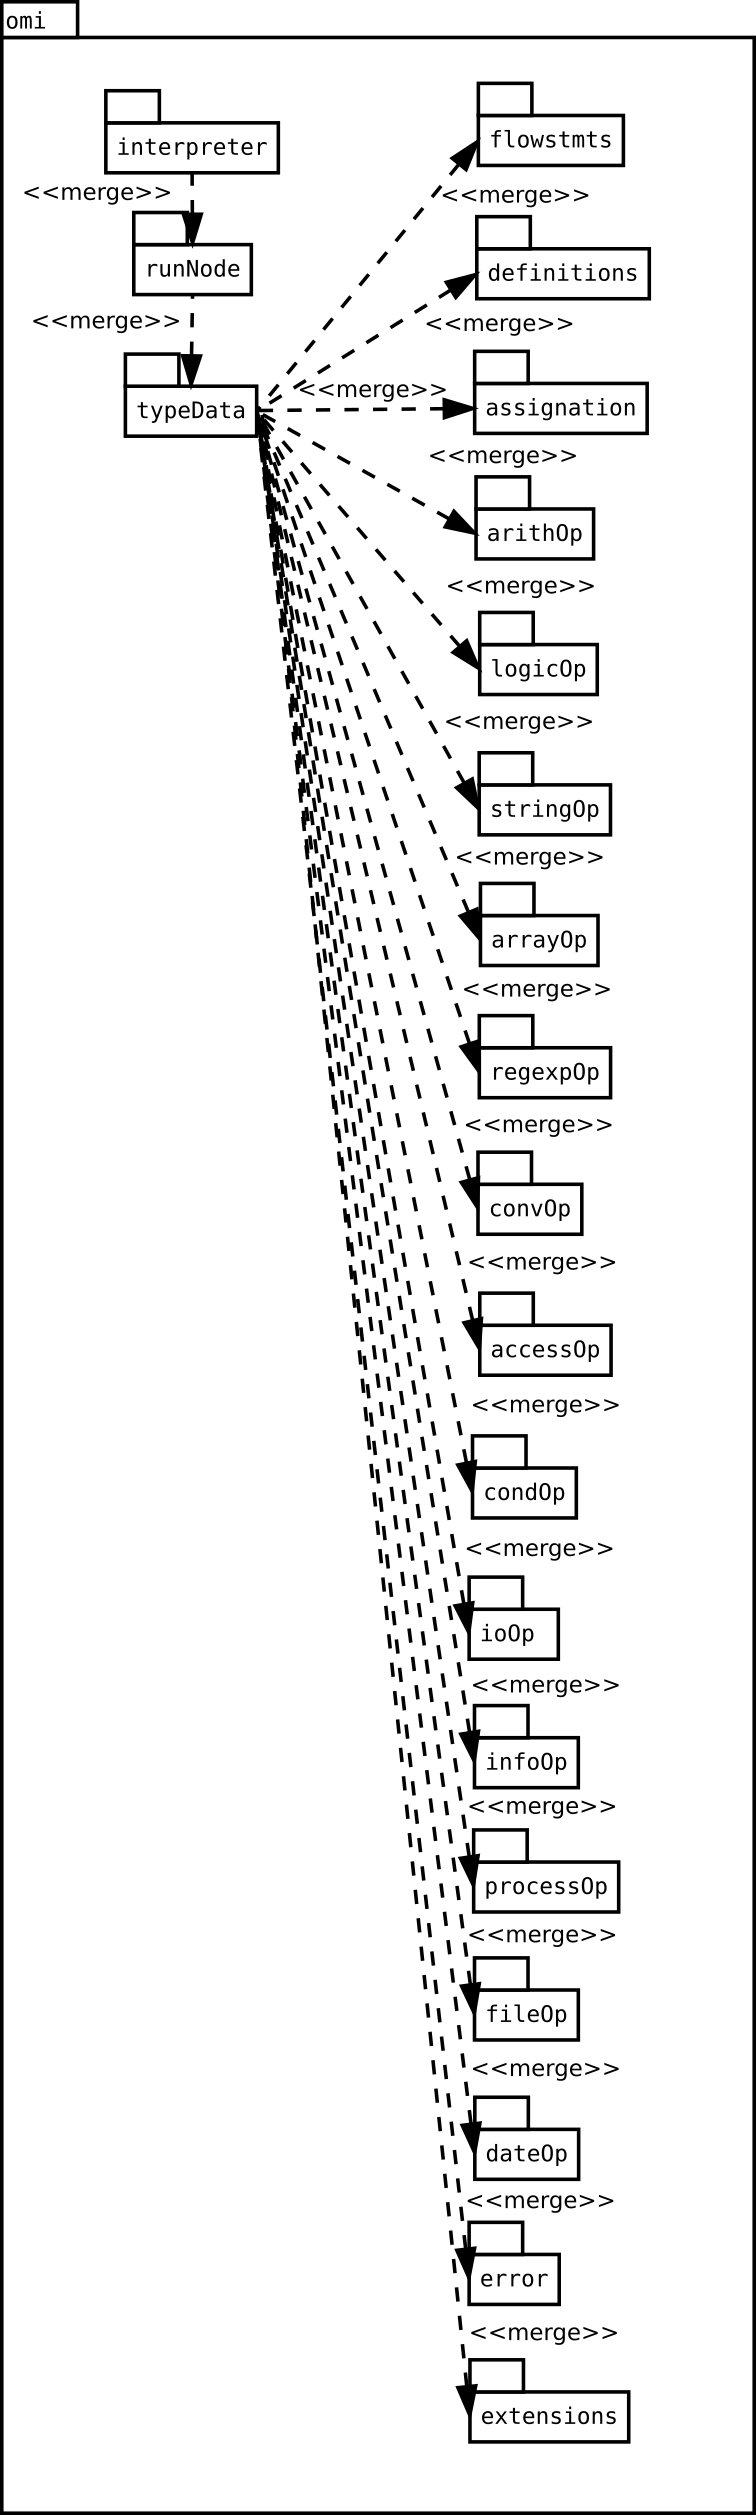
\includegraphics[scale=0.3]{analysis/package-omi.png}
\captionof{figure}{Paquetes OMI}
\end{center}
\end{multicols}
\pagebreak
Este árbol está formado 
por nodos denominados ejecutables, dado que al ser procesados en profundidad se llevará 
a cabo la ejecución del programa. Los nodos ejecutables dan significado semántico a 
cada una de las sentencias que componen el contenido fuente.

El interprete se compone además de un contexto denominado principal, que será sobre el que 
opere de forma predeterminada. Un contexto está formado por una serie de tablas de símbolos 
que serán manipuladas por ciertos nodos ejecutables cuando sean procesados. Estas tablas guardan 
referencias a nodos ejecutables correspondientes a símbolos variables, funciones y clases de objetos 
que son definidos en el código fuente. Existen determinados nodos que al ser ejecutados pueden 
cambiar el contexto en uso.

El interprete es ejecutado con una serie de argumentos que alteran su funcionamiento.

\begin{center}
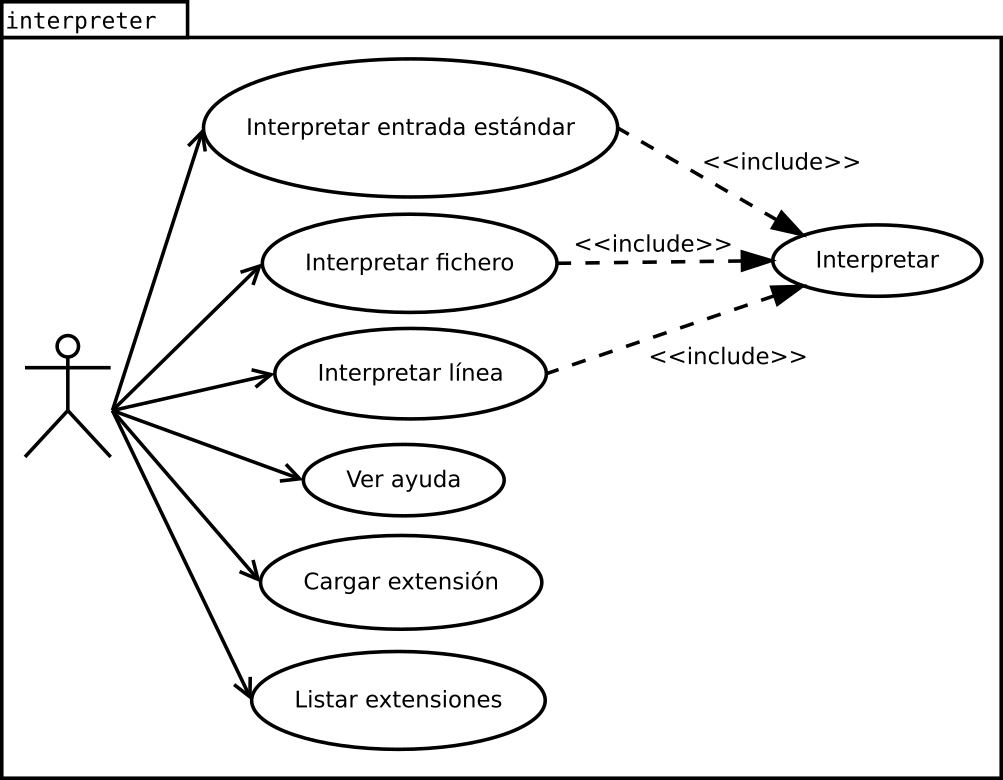
\includegraphics[scale=0.3]{analysis/interpreter.png}
\captionof{figure}{Clases intérprete}
\end{center}
% ----------------------------------------------------------------------
\subsection{Nodos ejecutables}
Se definen un nodo ejecutable para cada aspecto o funcionalidad que contemple el lenguaje.
Cada sentencia se corresponde con un nodo ejecutable, que a su vez puede estar compuestos de otros
nodos. Cada nodo ejecutable guarda el número de nodos que lo referencian para que se pueda hacer un uso 
óptimo del mismo.

Las expresiones son nodos ejecutables que tomarán un valor tras ser procesados. Generalmente forman parte de otros 
nodos correspondientes a sentencias u otras expresiones. El valor que toman pueden ser de un tipo determinado y conocido (numérico, lógico, etc), 
o de tipo indeterminado o no conocido hasta que el nodo es procesado. 

Las expresiones de tipo determinado son extendidas por cada tipo de dato soportado por el lenguaje. Además 
pueden ser consideradas tipos de objetos y estar así asociadas a una clase. De esta forma toda expresión puede disponer
de métodos y atributos según el tipo de dato que guarde.

Las expresiones de tipo indeterminado se componen de una referencia al nodo que guarda el valor tras la ejecución, este podrá ser una 
expresión de tipo determinado.

Las expresiones son nodos imprimibles lo que significa que tienen una representación gráfica asociada que puede ser volcada en la
salida estándar.

\begin{center}
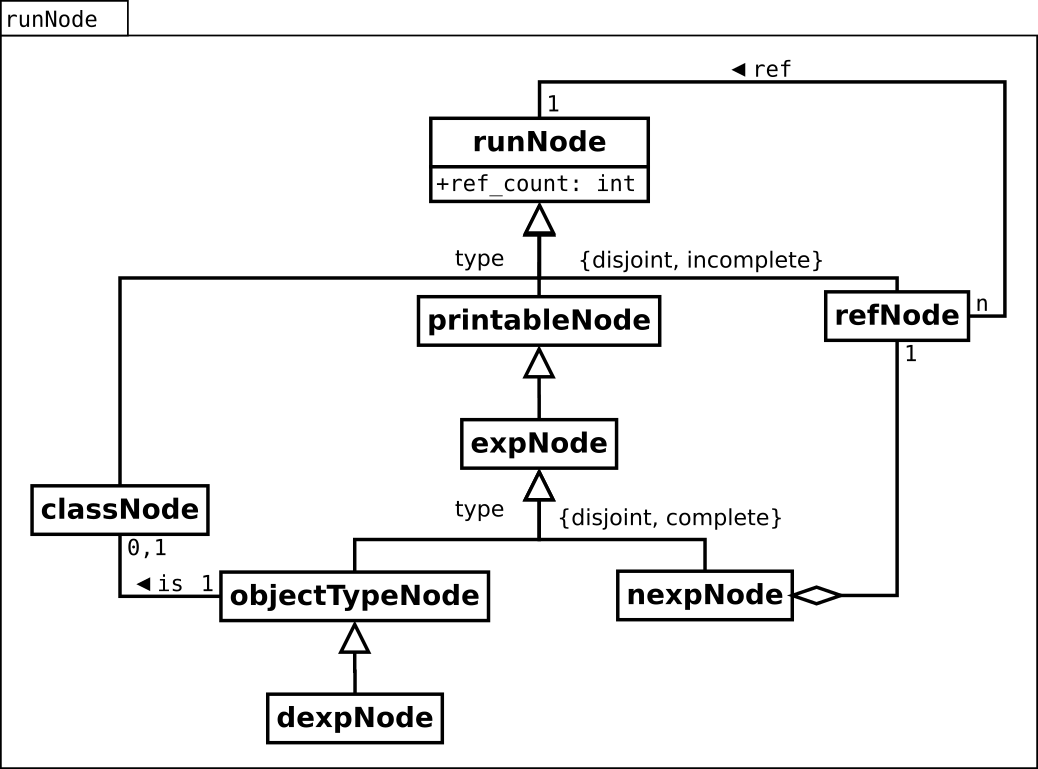
\includegraphics[scale=0.35]{analysis/runNode.png}
\captionof{figure}{Clases nodos ejecutables}
\end{center}
% ----------------------------------------------------------------------
\begin{multicols}{2}
\subsection{Tipos de datos}
Este paquete contiene los nodos que representan expresiones con tipos de datos definidos.
Se describe cada tipo de dato como un nodo con un valor asociado (en algunos casos el tipo puede comprender un único valor).

Muchos nodos son especializaciones de tipos de datos, correspondiéndose con expresiones que 
guardan un valor del tipo de dato al que extienden. Así por ejemplo los nodos de operaciones aritméticas
generalmente extenderán al nodo del mismo tipo de dato. 

Algunos nodos de tipos datos son concretados por nodos que representan un valor constante de dicho tipo de dato.
\columnbreak
\begin{center}
\hfill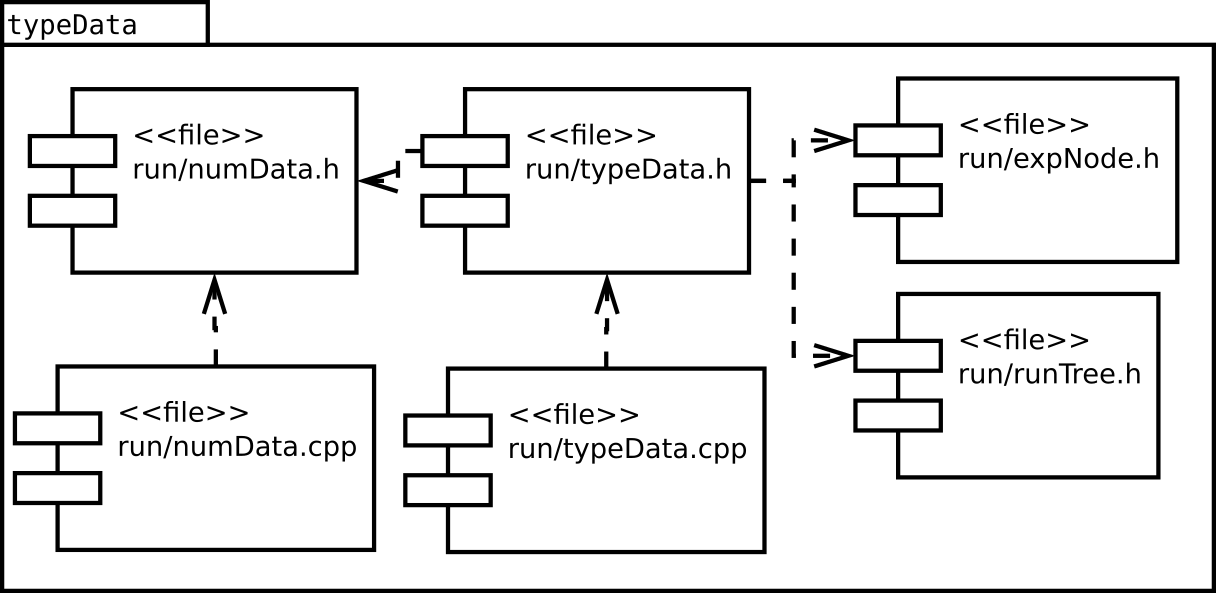
\includegraphics[scale=0.25]{analysis/typeData.png}
\captionof{figure}{Clases tipos de datos}
\end{center}
\end{multicols}
% ----------------------------------------------------------------------

\subsection{Sentencias de control de flujo}
\begin{center}
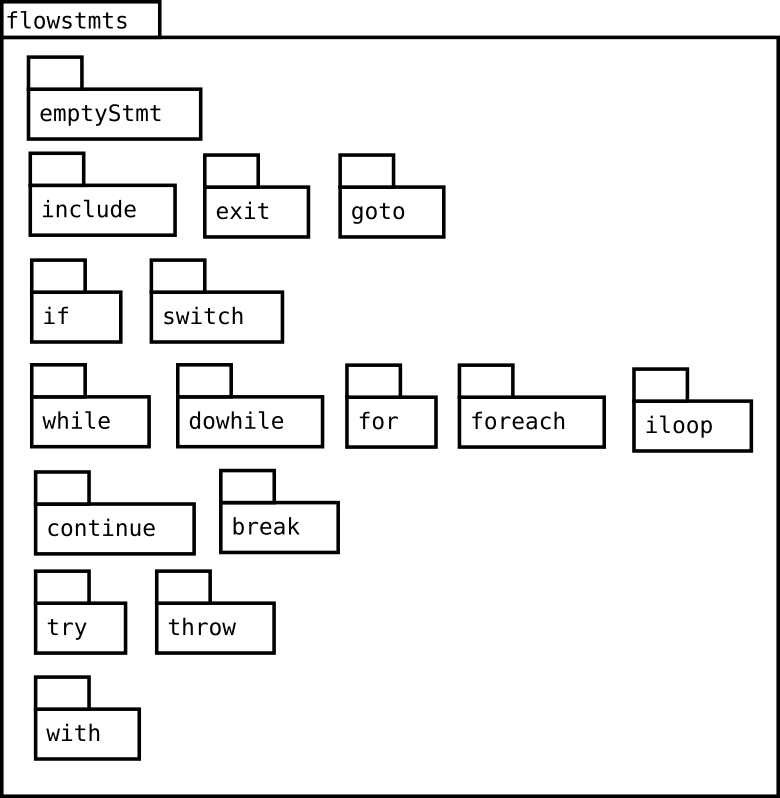
\includegraphics[scale=0.3]{analysis/flowstmts.png}
\captionof{figure}{Paquetes sentencias de control de flujo}
\end{center}

%~ \subsubsection{Sentencia}
\begin{multicols}{2}
\begin{center}
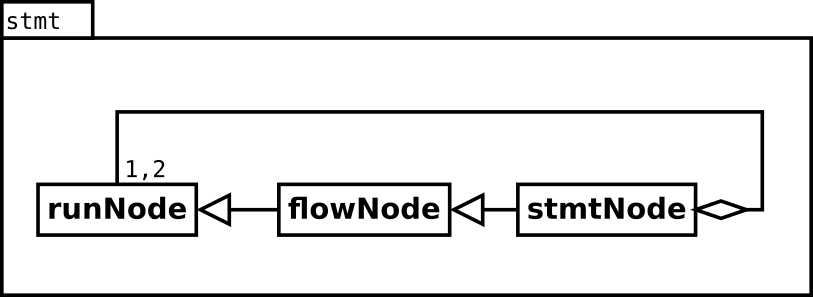
\includegraphics[scale=0.4]{analysis/stmt.png} 
\captionof{figure}{Clases sentencia}
\end{center}
\columnbreak
\begin{center}
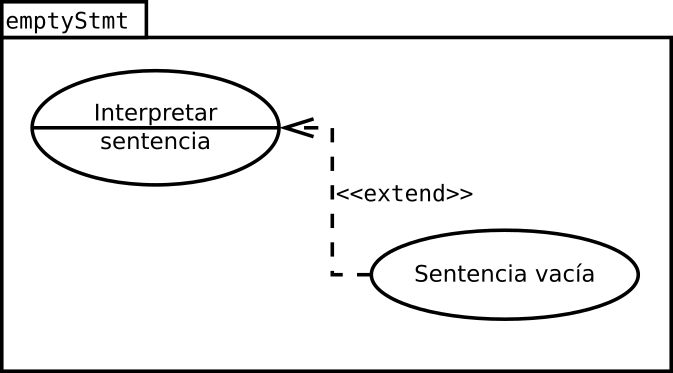
\includegraphics[scale=0.4]{analysis/emptyStmt.png} 
\captionof{figure}{Clases sentencia vacía}
\end{center}
\end{multicols}

\begin{multicols}{2}
%~ \subsubsection{include}
\begin{center}
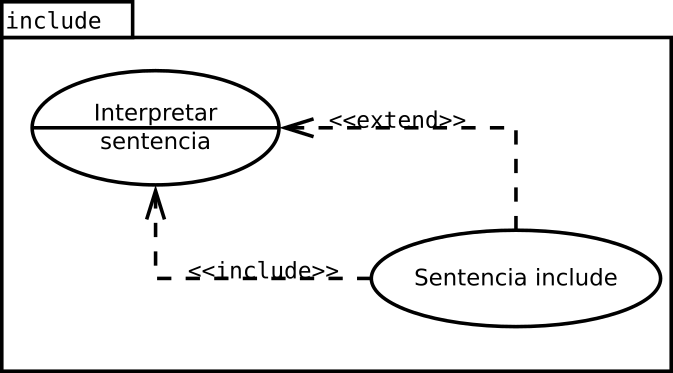
\includegraphics[scale=0.4]{analysis/include.png} 
\captionof{figure}{Clases include}
\end{center}
\columnbreak
%~ \subsubsection{exit}
\begin{center}
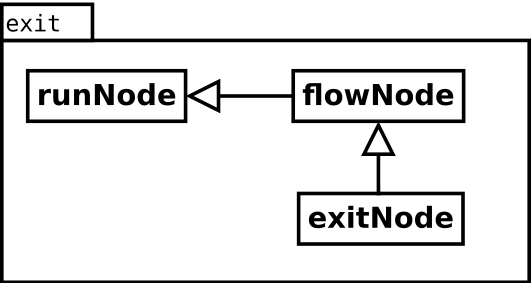
\includegraphics[scale=0.4]{analysis/exit.png} 
\captionof{figure}{Clases exit}
\end{center}
\end{multicols}

\begin{multicols}{2}
%~ \subsubsection{goto}
\begin{center}
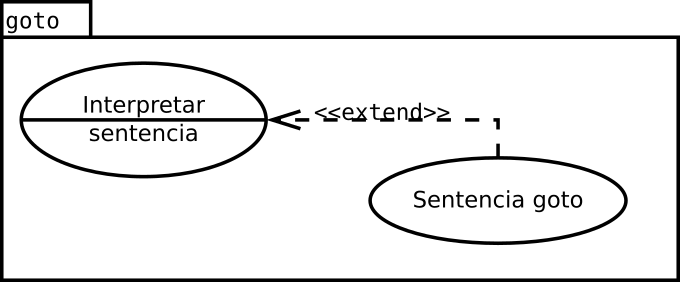
\includegraphics[scale=0.4]{analysis/goto.png} 
\captionof{figure}{Clases goto}
\end{center}
\columnbreak
%~ \subsubsection{if}
\begin{center}
\includegraphics[scale=0.4]{analysis/if.png} 
\captionof{figure}{Clases if}
\end{center}
\end{multicols}

\pagebreak
\begin{multicols}{2}
%~ \subsubsection{switch}
\begin{center}
\includegraphics[scale=0.4]{analysis/switch.png} 
\captionof{figure}{Clases switch}
\end{center}
\columnbreak
%~ \subsubsection{while}
\begin{center}
\includegraphics[scale=0.4]{analysis/while.png} 
\captionof{figure}{Clases while}
\end{center}
\end{multicols}

\begin{multicols}{2}
%~ \subsubsection{do...while}
\begin{center}
\includegraphics[scale=0.4]{analysis/dowhile.png} 
\captionof{figure}{Clases do...while}
\end{center}
\columnbreak
%~ \subsubsection{for}
\begin{center}
\includegraphics[scale=0.4]{analysis/for.png} 
\captionof{figure}{Clases for}
\end{center}
\end{multicols}

\begin{multicols}{2}
%~ \subsubsection{foreach}
\begin{center}
\includegraphics[scale=0.4]{analysis/foreach.png} 
\captionof{figure}{Clases foreach}
\end{center}
\columnbreak
%~ \subsubsection{iloop}
\begin{center}
\includegraphics[scale=0.4]{analysis/iloop.png} 
\captionof{figure}{Clases iloop}
\end{center}
\end{multicols}

\begin{multicols}{2}
%~ \subsubsection{continue}
\begin{center}
\includegraphics[scale=0.4]{analysis/continue.png} 
\captionof{figure}{Clases continue}
\end{center}
\columnbreak
%~ \subsubsection{break}
\begin{center}
\includegraphics[scale=0.4]{analysis/break.png} 
\captionof{figure}{Clases break}
\end{center}
\end{multicols}

\begin{multicols}{2}
%~ \subsubsection{try}
\begin{center}
\includegraphics[scale=0.4]{analysis/try.png} 
\captionof{figure}{Clases try}
\end{center}
\columnbreak
%~ \subsubsection{throw}
\begin{center}
\includegraphics[scale=0.4]{analysis/throw.png} 
\captionof{figure}{Clases throw}
\end{center}
\end{multicols}

%~ \subsubsection{with}
\begin{center}
\includegraphics[scale=0.4]{analysis/with.png} 
\captionof{figure}{Clases witch}
\end{center}
% ----------------------------------------------------------------------
\subsection {Definiciones}
\begin{center}
\includegraphics[scale=0.35]{analysis/definitions.png} 
\captionof{figure}{Paquetes definiciones}
\end{center}

%~ \subsubsection {Variables}
\begin{center}
\includegraphics[scale=0.35]{analysis/id.png} 
\captionof{figure}{Clases sobre variables}
\end{center}

%~ \subsubsection {Funciones}
\begin{center}
\includegraphics[scale=0.35]{analysis/functions.png} 
\captionof{figure}{Clases sobre funciones}
\end{center}

%~ \subsubsection {Clases}
\begin{center}
\includegraphics[scale=0.35]{analysis/class.png} 
\captionof{figure}{Clases sobre clases}
\end{center}
\pagebreak

\begin{multicols}{2}
%~ \subsubsection {Objetos}
\begin{center}
\includegraphics[scale=0.3]{analysis/object.png} 
\captionof{figure}{Clases sobre objetos}
\end{center}
\columnbreak
%~ \subsubsection {Listas}
\begin{center}
\includegraphics[scale=0.3]{analysis/list.png} 
\captionof{figure}{Clases sobre listas}
\end{center}
\end{multicols}

\begin{multicols}{2}
%~ \subsubsection {Pares clave/valor}
\begin{center}
\includegraphics[scale=0.3]{analysis/map.png} 
\captionof{figure}{Clases sobre pares clave/valor}
\end{center}
\columnbreak
%~ \subsubsection {Etiquetas}
\begin{center}
\includegraphics[scale=0.3]{analysis/label.png} 
\captionof{figure}{Etiquetas}
\end{center}
\end{multicols}

\begin{multicols}{2}
%~ \subsubsection {Definiciones globales}
\begin{center}
\includegraphics[scale=0.3]{analysis/global.png} 
\captionof{figure}{Definiciones globales}
\end{center}
\columnbreak
%~ \subsubsection {Generadores}
\begin{center}
\includegraphics[scale=0.3]{analysis/generator.png} 
\captionof{figure}{Clases sobre generadores}
\end{center}
\end{multicols}
% ----------------------------------------------------------------------

\subsection {Asignaciones}
\begin{center}
\includegraphics[scale=0.4]{analysis/assig-package.png} 
\captionof{figure}{Paquetes asignaciones}
\end{center}

\begin{multicols}{2}
%~ \subsubsection {Asignación}
\begin{center}
\includegraphics[scale=0.3]{analysis/assigNode.png} 
\captionof{figure}{Clases asignación}
\end{center}
\columnbreak
%~ \subsubsection {Asignación de referencia}
\begin{center}
\includegraphics[scale=0.3]{analysis/assigRef.png} 
\captionof{figure}{Clases asignación de referencia}
\end{center}
\end{multicols}

% ----------------------------------------------------------------------
\subsection {Operadores aritméticos}
\begin{center}
\includegraphics[scale=0.4]{analysis/arithOp-package.png} 
\captionof{figure}{Paquetes operadores aritméticos}
\end{center}

\begin{multicols}{2}
%~ \subsubsection {Suma}
\begin{center}
\includegraphics[scale=0.3]{analysis/add.png} 
\captionof{figure}{Clases suma}
\end{center}
\columnbreak
%~ \subsubsection {Diferencia}
\begin{center}
\includegraphics[scale=0.3]{analysis/sub.png} 
\captionof{figure}{Clases diferencia}
\end{center}
\end{multicols}

\begin{multicols}{2}
%~ \subsubsection {Producto}
\begin{center}
\includegraphics[scale=0.3]{analysis/prod.png} 
\captionof{figure}{Clases producto}
\end{center}
\columnbreak
%~ \subsubsection {División}
\begin{center}
\includegraphics[scale=0.3]{analysis/div.png} 
\captionof{figure}{Clases división}
\end{center}
\end{multicols}
\pagebreak

\begin{multicols}{2}
%~ \subsubsection {Potencia}
\begin{center}
\includegraphics[scale=0.3]{analysis/pow.png} 
\captionof{figure}{Clases potencia}
\end{center}
\columnbreak
%~ \subsubsection {Módulo}
\begin{center}
\includegraphics[scale=0.3]{analysis/mod.png} 
\captionof{figure}{Clases módulo}
\end{center}
\end{multicols}

\begin{multicols}{2}
%~ \subsubsection {Tamaño}
\begin{center}
\includegraphics[scale=0.3]{analysis/size.png} 
\captionof{figure}{Clases tamaño}
\end{center}
\columnbreak
%~ \subsubsection {Incremento y asignación}
\begin{center}
\includegraphics[scale=0.3]{analysis/incAssig.png} 
\captionof{figure}{Clases incremento y asignación}
\end{center}
\end{multicols}

\begin{multicols}{2}
%~ \subsubsection {Asignación e incremento}
\begin{center}
\includegraphics[scale=0.3]{analysis/assigInc.png} 
\captionof{figure}{Clases asignación e incremento}
\end{center}
\columnbreak
%~ \subsubsection {Decremento y asignación}
\begin{center}
\includegraphics[scale=0.3]{analysis/decAssig.png} 
\captionof{figure}{Clases decremento y asignación}
\end{center}
\end{multicols}

%~ \subsubsection {Asignación y decremento}
\begin{center}
\includegraphics[scale=0.3]{analysis/assigDec.png} 
\captionof{figure}{Clases asignación y decremento}
\end{center}
% ----------------------------------------------------------------------

 \subsection {Operadores lógicos}
 \begin{center}
\includegraphics[scale=0.4]{analysis/logicOp-package.png} 
\captionof{figure}{Paquetes operadores lógicos}
\end{center}

\begin{multicols}{2}
%~ \subsubsection {Or}
\begin{center}
\includegraphics[scale=0.3]{analysis/or.png} 
\captionof{figure}{Clases or}
\end{center}
\columnbreak
%~ \subsubsection {And}
\begin{center}
\includegraphics[scale=0.3]{analysis/and.png} 
\captionof{figure}{Clases and}
\end{center}
\end{multicols}

\begin{multicols}{2}
%~ \subsubsection {Negación}
\begin{center}
\includegraphics[scale=0.3]{analysis/not.png} 
\captionof{figure}{Clases negación}
\end{center}
\columnbreak
%~ \subsubsection {Igual que}
\begin{center}
\includegraphics[scale=0.3]{analysis/eq.png} 
\captionof{figure}{Clases igual que}
\end{center}
\end{multicols}
\pagebreak

\begin{multicols}{2}
%~ \subsubsection {Distinto que}
\begin{center}
\includegraphics[scale=0.3]{analysis/neq.png} 
\captionof{figure}{Clases distinto que}
\end{center}
\columnbreak
%~ \subsubsection {Menor que}
\begin{center}
\includegraphics[scale=0.3]{analysis/lth.png} 
\captionof{figure}{Clases menor que}
\end{center}
\end{multicols}

\begin{multicols}{2}
%~ \subsubsection {Menor o igual que}
\begin{center}
\includegraphics[scale=0.3]{analysis/leq.png} 
\captionof{figure}{Clases menor o igual que}
\end{center}
\columnbreak
%~ \subsubsection {Mayor que}
\begin{center}
\includegraphics[scale=0.3]{analysis/gth.png} 
\captionof{figure}{Clases mayor que}
\end{center}
\end{multicols}

\begin{multicols}{2}
%~ \subsubsection {Mayor o igual que}
\begin{center}
\includegraphics[scale=0.3]{analysis/geq.png} 
\captionof{figure}{Clases mayor o igual que}
\end{center}
\columnbreak
%~ \subsubsection {Idéntico a}
\begin{center}
\includegraphics[scale=0.3]{analysis/iden.png} 
\captionof{figure}{Clases idéntico a}
\end{center}
\end{multicols}

\begin{multicols}{2}
%~ \subsubsection {No idéntico a}
\begin{center}
\includegraphics[scale=0.3]{analysis/niden.png} 
\captionof{figure}{Clases no idéntico a}
\end{center}
\columnbreak
%~ \subsubsection {Es nulo}
\begin{center}
\includegraphics[scale=0.3]{analysis/isNull.png} 
\captionof{figure}{Clases es nulo}
\end{center}
\end{multicols}

%~ \subsubsection {Vacío}
\begin{center}
\includegraphics[scale=0.3]{analysis/empty.png} 
\captionof{figure}{Clases vacío}
\end{center}

% ----------------------------------------------------------------------

\subsection {Operadores sobre cadenas}
\begin{center}
\includegraphics[scale=0.3]{analysis/stringOp-package.png} 
\captionof{figure}{Paquetes operadores de cadenas}
\end{center}

\begin{multicols}{2}
%~ \subsubsection {Concatenación}
\begin{center}
\includegraphics[scale=0.3]{analysis/cat.png} 
\captionof{figure}{Clases concatenación}
\end{center}
\columnbreak
%~ \subsubsection {explode}
\begin{center}
\includegraphics[scale=0.3]{analysis/explode.png} 
\captionof{figure}{Clases explode}
\end{center}
\end{multicols}

\begin{multicols}{2}
%~ \subsubsection {implode}
\begin{center}
\includegraphics[scale=0.3]{analysis/implode.png} 
\captionof{figure}{Clases implode}
\end{center}
\columnbreak
%~ \subsubsection {sprintf}
\begin{center}
\includegraphics[scale=0.3]{analysis/sprintf.png} 
\captionof{figure}{Clases sprintf}
\end{center}
\end{multicols}

\begin{multicols}{2}
%~ \subsubsection {Buscar subcadena}
\begin{center}
\includegraphics[scale=0.3]{analysis/find.png} 
\captionof{figure}{Clases buscar subcadena}
\end{center}
\columnbreak
%~ \subsubsection {Buscar y remplazar}
\begin{center}
\includegraphics[scale=0.3]{analysis/replace.png} 
\captionof{figure}{Clases buscar y remplazar}
\end{center}
\end{multicols}

\begin{multicols}{2}
%~ \subsubsection {Remplazar subcadena}
\begin{center}
\includegraphics[scale=0.3]{analysis/subreplace.png} 
\captionof{figure}{Clases remplazar subcadena}
\end{center}
\columnbreak
%~ \subsubsection {Convertir a mayúsculas}
\begin{center}
\includegraphics[scale=0.3]{analysis/upper.png}
\captionof{figure}{Clases convertir a mayúsculas} 
\end{center}
\end{multicols}

%~ \subsubsection {Convertir a minúsculas}
\begin{center}
\includegraphics[scale=0.3]{analysis/lower.png} 
\captionof{figure}{Clases convertir a minúsculas} 
\end{center}

%~ \subsubsection {Concatenación y asignación}
%~ Diagrama aún por realizar.
%~ \begin{center}
%~ \includegraphics[scale=0.4]{analysis/lower.png} \\
%~ \end{center}
% ----------------------------------------------------------------------

\subsection {Operadores sobre array}
\begin{center}
\includegraphics[scale=0.4]{analysis/arrayOp-package.png} 
\captionof{figure}{Paquetes operadores sobre array} 
\end{center}

\begin{multicols}{2}
%~ \subsubsection {Dividir en fragmentos}
\begin{center}
\includegraphics[scale=0.25]{analysis/chunk.png} 
\captionof{figure}{Clases dividir en fragmentos} 
\end{center}
\columnbreak
%~ \subsubsection {Reducir mediante función}
\begin{center}
\includegraphics[scale=0.25]{analysis/reduce.png} 
\captionof{figure}{Clases reducir mediante función} 
\end{center}
\end{multicols}

\begin{multicols}{2}
%~ \subsubsection {Obtener último}
\begin{center}
\includegraphics[scale=0.35]{analysis/last.png} 
\captionof{figure}{Clases obtener último} 
\end{center}
\columnbreak
%~ \subsubsection {Obtener primero}
\begin{center}
\includegraphics[scale=0.35]{analysis/first.png} 
\captionof{figure}{Clases obtener primero} 
\end{center}
\end{multicols}

\begin{multicols}{2}
%~ \subsubsection {Insertar en posición}
\begin{center}
\includegraphics[scale=0.35]{analysis/insert.png} 
\captionof{figure}{Clases insertar en posición} 
\end{center}
\columnbreak
%~ \subsubsection {Eliminar posición}
\begin{center}
\includegraphics[scale=0.35]{analysis/delete.png} 
\captionof{figure}{Clases eliminar posición} 
\end{center}
\end{multicols}

\begin{multicols}{2}
%~ \subsubsection {Insertar al inicio}
\begin{center}
\includegraphics[scale=0.35]{analysis/unshift.png} 
\captionof{figure}{Clases insertar al inicio}
\end{center}
\columnbreak
%~ \subsubsection {Insertar al final}
\begin{center}
\includegraphics[scale=0.35]{analysis/push.png} 
\captionof{figure}{Clases insertar al final}
\end{center}
\end{multicols}

\begin{multicols}{2}
%~ \subsubsection {Eliminar del inicio}
\begin{center}
\includegraphics[scale=0.35]{analysis/shift.png} 
\captionof{figure}{Clases eliminar del inicio}
\end{center}
\columnbreak
%~ \subsubsection {Eliminar del final}
\begin{center}
\includegraphics[scale=0.35]{analysis/pop.png} 
\captionof{figure}{Clases eliminar del final}
\end{center}
\end{multicols}

% ----------------------------------------------------------------------

\subsection {Operadores sobre expresiones regulares}
\begin{center}
\includegraphics[scale=0.4]{analysis/regexpOp-package.png} 
\captionof{figure}{Paquetes operadores sobre expresiones regulares}
\end{center}

\begin{multicols}{2}
%~ \subsubsection {Crear expresión regular}
\begin{center}
\includegraphics[scale=0.25]{analysis/newRegExp.png}
\captionof{figure}{Clases crear expresión regular} 
\end{center}
\columnbreak
%~ \subsubsection {match}
\begin{center}
\includegraphics[scale=0.3]{analysis/match.png} 
\captionof{figure}{Clases match}
\end{center}
\end{multicols}

%~ \subsubsection {search}
\begin{center}
\includegraphics[scale=0.3]{analysis/search.png} 
\captionof{figure}{Clases search}
\end{center}

% ----------------------------------------------------------------------

\subsection {Conversión de tipos}
\begin{center}
\includegraphics[scale=0.3]{analysis/convOp-package.png} 
\captionof{figure}{Paquetes conversión de tipos}
\end{center}

\begin{multicols}{2}
%~ \subsubsection {Conversión a lógico}
\begin{center}
\includegraphics[scale=0.35]{analysis/boolconv.png} 
\captionof{figure}{Clases conversión a lógico}
\end{center}
\columnbreak
%~ \subsubsection {Conversión a entero}
\begin{center}
\includegraphics[scale=0.35]{analysis/intconv.png} 
\captionof{figure}{Clases conversión a entero}
\end{center}
\end{multicols}

\begin{multicols}{2}
%~ \subsubsection {Conversión a flotante}
\begin{center}
\includegraphics[scale=0.35]{analysis/floatconv.png} 
\captionof{figure}{Clases conversión a flotante}
\end{center}
\columnbreak
%~ \subsubsection {Conversión a cadena}
\begin{center}
\includegraphics[scale=0.35]{analysis/strconv.png} 
\captionof{figure}{Clases conversión a cadena}
\end{center}
\end{multicols}
% ----------------------------------------------------------------------

\subsection {Operadores de acceso}
\begin{center}
\includegraphics[scale=0.4]{analysis/accessOp-package.png} 
\captionof{figure}{Paquetes operadores de acceso}
\end{center}

\begin{multicols}{2}
%~ \subsubsection {Acceso a clave} 
\begin{center}
\includegraphics[scale=0.3]{analysis/get.png} 
\captionof{figure}{Clases acceso a clave}
\end{center}
\columnbreak
%~ \subsubsection {Acceso a función} 
\begin{center}
\includegraphics[scale=0.3]{analysis/getFunc.png} 
\captionof{figure}{Clases acceso a función}
\end{center}
\end{multicols}

%~ \subsubsection {Acceso a variable de entorno} 
\begin{center}
\includegraphics[scale=0.3]{analysis/getEnvSys.png} 
\captionof{figure}{Clases acceso a variable de entorno}
\end{center}
% ----------------------------------------------------------------------

\subsection {Operadores condicionales} 
\begin{center}
\includegraphics[scale=0.4]{analysis/condOp-package.png} 
\captionof{figure}{Paquetes Operadores condicionales}
\end{center}

\begin{multicols}{2}
%~ \subsubsection {Ternario} 
\begin{center}
\includegraphics[scale=0.3]{analysis/tern.png} 
\captionof{figure}{Clases ternario}
\end{center}
\columnbreak
%~ \subsubsection {Fusión de nulos} 
\begin{center}
\includegraphics[scale=0.3]{analysis/nullCoalescing.png} 
\captionof{figure}{Clases fusión de nulos}
\end{center}
\end{multicols}

% ----------------------------------------------------------------------

\subsection {Operadores de entrada/salida} 
\begin{center}
\includegraphics[scale=0.4]{analysis/ioOp-package.png} 
\captionof{figure}{Paquetes operadores de entrada/salida}
\end{center}

\pagebreak
\begin{multicols}{2}
%~ \subsubsection {Salida estándar} 
\begin{center}
\includegraphics[scale=0.3]{analysis/output.png} 
\captionof{figure}{Clases salida estándar}
\end{center}
\columnbreak
%~ \subsubsection {Entrada estándar} 
\begin{center}
\includegraphics[scale=0.3]{analysis/input.png} 
\captionof{figure}{Clases entrada estándar}
\end{center}
\end{multicols}

% ----------------------------------------------------------------------

\subsection {Operadores informativos} 
\begin{center}
\includegraphics[scale=0.4]{analysis/infoOp-package.png} 
\captionof{figure}{Paquetes operadores informativos}
\end{center}

\begin{multicols}{2}
%~ \subsubsection {Tipo de} 
\begin{center}
\includegraphics[scale=0.3]{analysis/typeOf.png} 
\captionof{figure}{Clases tipo de}
\end{center}
\columnbreak
%~ \subsubsection {Tamaño de} 
\begin{center}
\includegraphics[scale=0.3]{analysis/sizeOf.png} 
\captionof{figure}{Clases tamaño de}
\end{center}
\end{multicols}

%~ \subsubsection {Información sobre} 
\begin{center}
\includegraphics[scale=0.3]{analysis/datInfo.png} 
\captionof{figure}{Clases información sobre}
\end{center}
% ----------------------------------------------------------------------

\subsection {Procesos} 
\begin{center}
\includegraphics[scale=0.4]{analysis/processOp-package.png} 
\captionof{figure}{Paquete de procesos}
\end{center}

\begin{multicols}{2}
%~ \subsubsection {Crear proceso} 
\begin{center}
\includegraphics[scale=0.3]{analysis/fork.png} 
\captionof{figure}{Clases crear proceso}
\end{center}
\columnbreak
%~ \subsubsection {Esperar finalización} 
\begin{center}
\includegraphics[scale=0.3]{analysis/wait.png} 
\captionof{figure}{Clases esperar finalización}
\end{center}
\end{multicols}

\begin{multicols}{2}
%~ \subsubsection {Obtener identificador } 
\begin{center}
\includegraphics[scale=0.3]{analysis/getpid.png} 
\captionof{figure}{Clases obtener identificador}
\end{center}
\columnbreak
%~ \subsubsection {Obtener identificador padre} 
\begin{center}
\includegraphics[scale=0.3]{analysis/getppid.png} 
\captionof{figure}{Clases obtener identificador padre}
\end{center}
\end{multicols}

\begin{multicols}{2}
%~ \subsubsection {Ejecutar como proceso} 
\begin{center}
\includegraphics[scale=0.3]{analysis/process.png} 
\captionof{figure}{Clases ejecutar como proceso}
\end{center}
\columnbreak
%~ \subsubsection {Salir de proceso} 
\begin{center}
\includegraphics[scale=0.3]{analysis/exitProcess.png} 
\captionof{figure}{Clases salir de proceso}
\end{center}
\end{multicols}

\pagebreak

\begin{multicols}{2}
%~ \subsubsection {Señal a proceso} 
\begin{center}
\includegraphics[scale=0.3]{analysis/signal.png} 
\captionof{figure}{Clases señal a proceso}
\end{center}
\columnbreak
%~ \subsubsection {Manejador de señales} 
\begin{center}
\includegraphics[scale=0.3]{analysis/signalhandler.png} 
\captionof{figure}{Clases manejador de señales}
\end{center}
\end{multicols}

\begin{multicols}{2}
%~ \subsubsection {Evaluar cadena} 
\begin{center}
\includegraphics[scale=0.3]{analysis/eval.png} 
\captionof{figure}{Clases evaluar cadena}
\end{center}
\columnbreak
%~ \subsubsection {Ejecutar comando del sistema} 
\begin{center}
\includegraphics[scale=0.3]{analysis/exec.png} 
\captionof{figure}{Clases ejecutar comando del sistema}
\end{center}
\end{multicols}
% ----------------------------------------------------------------------

\subsection {Ficheros} 
\begin{center}
\includegraphics[scale=0.4]{analysis/fileOp-package.png} 
\captionof{figure}{Paquetes de ficheros}
\end{center}

\begin{multicols}{2}
%~ \subsubsection {Obtener un flujo a fichero} 
\begin{center}
\includegraphics[scale=0.3]{analysis/file.png} 
\captionof{figure}{Clases obtener un flujo a fichero}
\end{center}
\columnbreak
%~ \subsubsection {Escribir en flujo a fichero} 
\begin{center}
\includegraphics[scale=0.3]{analysis/fput.png} 
\captionof{figure}{escribir en flujo a fichero}
\end{center}
\end{multicols}

\begin{multicols}{2}
%~ \subsubsection {Leer de flujo a fichero} 
\begin{center}
\includegraphics[scale=0.3]{analysis/fget.png} 
\captionof{figure}{Clases leer de flujo a fichero}
\end{center}
\columnbreak
%~ \subsubsection {Cambiar posición en fichero} 
\begin{center}
\includegraphics[scale=0.3]{analysis/fseek.png} 
\captionof{figure}{Clases cambiar posición en fichero}
\end{center}
\end{multicols}

\begin{multicols}{2}
%~ \subsubsection {Obtener posición en flujo a fichero} 
\begin{center}
\includegraphics[scale=0.3]{analysis/ftell.png} 
\captionof{figure}{Clases obtener posición en flujo a fichero}
\end{center}
\columnbreak
%~ \subsubsection {Cerrar flujo a fichero} 
\begin{center}
\includegraphics[scale=0.3]{analysis/fclose.png} 
\captionof{figure}{Clases cerrar flujo a fichero}
\end{center}
\end{multicols}

\begin{multicols}{2}
%~ \subsubsection {Leer fichero} 
\begin{center}
\includegraphics[scale=0.3]{analysis/fread.png} 
\captionof{figure}{Clases leer fichero}
\end{center}
\columnbreak
%~ \subsubsection {Escribir en fichero} 
\begin{center}
\includegraphics[scale=0.3]{analysis/fwrite.png} 
\captionof{figure}{Clases escribir en fichero}
\end{center}
\end{multicols}

%~ \subsubsection {Escribir al final de fichero} 
\begin{center}
\includegraphics[scale=0.3]{analysis/fappend.png} 
\captionof{figure}{Clases escribir al final de fichero}
\end{center}
% ----------------------------------------------------------------------
 \pagebreak

\subsection {Fechas}
\begin{center}
\includegraphics[scale=0.4]{analysis/dateOp-package.png} 
\captionof{figure}{Paquetes de fechas}
\end{center}

\begin{multicols}{2}
%~ \subsubsection {Tiempo Unix} 
\begin{center}
\includegraphics[scale=0.35]{analysis/time.png} 
\captionof{figure}{Clases tiempo Unix}
\end{center}
\columnbreak
%~ \subsubsection {Fecha y hora con formato} 
\begin{center}
\includegraphics[scale=0.35]{analysis/date.png} 
\captionof{figure}{Clases fecha y hora con formato}
\end{center}
\end{multicols}

%~ \subsubsection {sleep} 
\begin{center}
\includegraphics[scale=0.35]{analysis/sleep.png} 
\captionof{figure}{Clases sleep}
\end{center}

% ----------------------------------------------------------------------

\subsection {Errores} 
%~ \begin{center}
%~ \includegraphics[scale=0.4]{analysis/error-package.png} \\
%~ \end{center}
%~ 
%~ \subsubsection {Error} 
\begin{center}
\includegraphics[scale=0.35]{analysis/errorException.png} 
\captionof{figure}{Clases Errores}
\end{center}

%~ \subsubsection {Manejador de errores } 
%~ Diagrama aún por realizar
%~ \begin{center}
%~ \includegraphics[scale=0.4]{analysis/errorhandler.png} \\
%~ \end{center}

%~ \subsubsection {Manejador de excepciones no capturadas} 
%~ Diagrama aún por realizar
%~ \begin{center}
%~ \includegraphics[scale=0.4]{analysis/errorhandler.png} \\
%~ \end{center}
% ----------------------------------------------------------------------


\subsection {Extensiones} 
\begin{center}
\includegraphics[scale=0.35]{analysis/extensions-package.png} 
\captionof{figure}{Paquete de extensiones}
\end{center}

%~ \subsection {plugins}
\begin{center}
\includegraphics[scale=0.35]{analysis/plugins.png} 
\captionof{figure}{Clases plugins}
\end{center}

\subsubsection{Biblioteca GNU de internacionalización (gettext)}
\begin{center}
\includegraphics[scale=0.4]{analysis/gettext-ext-package.png} 
\captionof{figure}{Paquetes de Biblioteca GNU de internacionalización (gettext)}
\end{center}

%~ \paragraph {gettext}
\begin{center}
\includegraphics[scale=0.35]{analysis/gettext.png} 
\captionof{figure}{Clases gettext}
\end{center}

\begin{multicols}{2}
%~ \paragraph {setlocale}
\begin{center}
\includegraphics[scale=0.35]{analysis/setlocale.png} 
\captionof{figure}{Clases setlocale}
\end{center}
%~ \paragraph {dgettext}
\begin{center}
\includegraphics[scale=0.35]{analysis/dgettext.png} 
\captionof{figure}{Clases dgettext}
\end{center}
\columnbreak
%~ \paragraph {bindtextdomain}
\begin{center}
\includegraphics[scale=0.35]{analysis/bindtextdomain.png} 
\captionof{figure}{Clases bindtextdomain}
\end{center}
%~ \paragraph {textdomain}
\begin{center}
\includegraphics[scale=0.35]{analysis/textdomain.png} 
\captionof{figure}{Clases textdomain}
\end{center}
\end{multicols}

\subsection {rTree} 
El intérprete OMI tiene la capacidad de generar una salida relativa
a su estado y funcionamiento. Para completar el proyecto se precisa 
de una herramienta capaz de interpretar y representar este estado 
interno de forma gráfica y textual. 

El modelo de datos del cliente OMI se define de forma similar al intérprete.
La principal diferencia es que en el intérprete este modelo de datos se usa para procesar y 
ejecutar el código fuente, mientras que en el cliente se usa para representar gráficamente 
el proceso llevado a cabo. Es por ello que el modelo de datos del cliente es más abstracto. 

\begin{center}
\includegraphics[scale=0.6]{analysis/rtree.png} 
\captionof{figure}{Clases rTree}
\end{center}

%~ \subsubsection {Operaciones sobre un SGBD Mysql}
%~ \begin{center}
%~ \includegraphics[scale=0.4]{analysis/mysql-ext-package.png} \\
%~ \end{center}
%~ \paragraph {Abrir conexión}
%~ \begin{center}
%~ \includegraphics[scale=0.4]{analysis/db.png} \\
%~ \end{center}
%~ 
%~ \paragraph {Consulta}
%~ \begin{center}
%~ \includegraphics[scale=0.4]{analysis/dbQuery.png} \\
%~ \end{center}
%~ 
%~ \paragraph {Cerrar conexión}
%~ Diagrama aún por realizar.
%~ \begin{center}
%~ \includegraphics[scale=0.4]{analysis/dbClose.png} \\
%~ \end{center}
%~ 
%~ \paragraph {Insertar datos}
%~ \begin{center}
%~ \includegraphics[scale=0.4]{analysis/dbInsert.png} \\
%~ \end{center}
%~ 
%~ \paragraph {Seleccionar datos}
%~ \begin{center}
%~ \includegraphics[scale=0.4]{analysis/dbSelect.png} \\
%~ \end{center}
%~ 
%~ \paragraph {Actualizar datos}
%~ \begin{center}
%~ \includegraphics[scale=0.4]{analysis/dbUpdate.png} \\
%~ \end{center}
%~ 
%~ \paragraph {Eliminar datos}
%~ \begin{center}
%~ \includegraphics[scale=0.4]{analysis/dbDelete.png} \\
%~ \end{center}
%~ 
%~ % ----------------------------------------------------------------------


% ======================================================================
\section{Modelo de casos de uso}
%~ En el presente documento se detallan los casos de uso recogidos para el 
%~ interprete OMI. Para ello los casos de uso son distribuidos
%~ en paquetes, y estos modelados mediante un diagrama. 
%~ 
%~ El diagrama de paquetes inicial presenta una organización y distribución 
%~ general de los paquetes en los que se ha dividido el modelo. Estos paquetes
%~ pueden contener diagramas de casos de uso u otros paquetes. Además se establecen
%~ relaciones entre estos.
%~ 
%~ La relación de mezcla (merge) entre dos paquetes significa que el contenido
%~ de ambos paquetes será superpuesto, cumplimentando la información que presenta uno
%~ con la que ofrece el otro. 
%~ 
%~ Inicialmente se presenta el paquete ``interpreter'' que recoge los casos 
%~ de uso que puede llevar a cabo el usuario. Aquí el caso de uso que cabría 
%~ destacar es el de Interpretar. Este consiste en la interpretación sentencia 
%~ a sentencia del código fuente facilitado por el usuario. Este caso de
%~ uso es extendido según el tipo de sentencia interpretada en cada momento.
En esta sección se detallan los casos de usos que recogen los sistemas que conforman el proyecto OMI. 
Un caso de uso describe la secuencia de  interacciones entre el sistema y sus
actores como consecuencia de un evento. 

En primer lugar se describen los actores que hacen uso del sistema, llegándose a distinguir dos que serán nominados 
usuario y sistema externo. Luego se describen los casos de uso del sistema intérprete y del cliente runTree. 

\subsection{Actores}
Los actores humanos que interactúan con los sistemas OMI presentan todos un mismo rol. Así el 
único actor definido será llamado usuario.  Los usuarios que hacen uso del intérprete pueden ser desarrolladores,
estudiantes u otros perfiles técnicos, pero todos usarán el sistema de la misma forma.

Por otro lado el intérprete OMI puede ser usado por otros sistemas, viéndose estos actores de determinados casos
de uso. Algunos sistemas del proyecto OMI hacen uso del intérprete para llevar  a cabo su propósito.

%~ En primer lugar se describen los casos de usos del intérprete OMI. El principal caso de uso es
%~ el de intérpretar, ya que recoge el proceso principal.  

%~ \begin{center}
%~ \includegraphics[scale=0.3]{analysis/package-omi.png} \\
%~ \end{center}
% ======================================================================
\subsection{Intérprete}
\begin{center}
\includegraphics[scale=0.5]{analysis/use_case_interpreter.png} 
\captionof{figure}{Casos de usos intérprete}
\end{center}
% ----------------------------------------------------------------------
\subsubsection{Casos de usos interpretar entrada estándar}

\begin{description}
  \item[Caso de Uso:] 
  Interpretar entrada estándar.
  \item[Tipo:] General.
  \item[Descripción:] 
  El usuario introduce un bloque de código en forma de cadena de 
  caracteres mediante la entrada estándar. El sistema lo interpreta 
  y ejecuta.
  \item[Actores:] 
  Usuario.
  \item[Precondiciones:] 
  El sistema debe estar esperando un bloque de código mediante la entrada estándar.
  \item[Postcondiciones:] 
  El código introducido es interpretado y ejecutado.
  \item[Escenario principal:] \hfill 
  \begin{enumerate}
   \item El usuario inicia el sistema facilitando un listado de argumentos.
   \item El sistema asigna como variables cada argumento y solicita contenido fuente al usuario. 
   \item El usuario introduce un bloque de código en la entrada estándar.
   \item El sistema obtiene el bloque de código a interpretar mediante la entrada estándar.
   \item Incluir (Interpretar). 
  \end{enumerate}
\end{description}
% ----------------------------------------------------------------------
\subsubsection{Interpretar fichero}

\begin{description}
   \item[Caso de Uso:]  Interpretar fichero.
   \item[Tipo:] General.
   \item[Descripción:] 
   El usuario indica un fichero que contiene código y que será 
   interpretado y ejecutado por el sistema.
   \item[Actores:] 
   Usuario.
   \item[Precondiciones:] 
   El sistema espera que se le indique un fichero.
   \item[Postcondiciones:] 
   El fichero es leído y el código en el mismo es interpretado y ejecutado.
   \item[Escenario principal:] \hfill
   \begin{enumerate}
   \item El usuario indica la ruta a un fichero y una serie de argumentos
   \item El sistema lee el fichero y obtiene el código en el mismo, además asigna cada argumento a variables.
   \item Incluir (Interpretar).
   \end{enumerate}
   
   \item[Flujo alternativo:] \hfill 
   \begin{enumerate} \itemsep1pt \parskip0pt \parsep0pt
   \setcounter{enumi}{1}
   \renewcommand{\labelenumi}{}
   \renewcommand{\labelenumiii}{\arabic{enumiii}.}
   \renewcommand{\labelenumii}{\arabic{enumi}\alph{enumii}.}
      \item 
      \begin {enumerate}
         \setcounter{enumii}{0}
         \item El fichero indicado no se encuentra.
         \begin{enumerate}
         \item El sistema informa del error y finaliza.
         \end{enumerate}
      \end{enumerate}
   \end{enumerate}
\end{description}

% ----------------------------------------------------------------------
\subsubsection{Interpretar línea}

\begin{description}
   \item[Caso de Uso:]  Interpretar línea.
   \item[Tipo:] General.
   \item[Descripción:] 
   El usuario introduce bloques de códigos denominados líneas
   de una forma interactiva. El sistema solicita por la entrada 
   estándar las líneas de código, que serán interpretadas y ejecutadas.
   \item[Actores:] 
   Usuario.
   \item[Precondiciones:] 
   El sistema se encuentra en modo interactivo.
   \item[Postcondiciones:] 
   Se interpreta cada línea introducida por el usuario
   \item[Escenario principal:] \hfill
   \begin{enumerate}
   \item El usuario inicia el sistema facilitando un listado de argumentos y la opción de interprete de línea.
   \item El sistema asigna como variables cada argumento y muestra un prompt que indica que espera una línea de código.
   \item El usuario introduce una línea de código.
   \item El sistema lee de la entrada estándar la línea introducida.
   \item Include (Interpretar). \\\\\hfill\hfill
   El sistema repite el caso de uso hasta que se interpreta una sentencia que produzca 
   la salida.
   \end{enumerate}
\end{description}

% ----------------------------------------------------------------------
\subsubsection{Interpretar}

\begin{description}
   \item[Caso de Uso:]  Interpretar.
   \item[Tipo:] General.
   \item[Nivel:]  Subfunción.
   \item[Descripción:] 
   El sistema analiza, interpreta y ejecuta un bloque de código facilitado por el usuario.
   Para ello comprueba que este cumple con el léxico y la gramática del lenguaje 
   que define, dividiéndolo a su vez en sentencias que serán interpretadas. 
   \item[Precondiciones:] 
   Se dispone de un bloque de código.
   \item[Postcondiciones:] 
   El bloque de código es interpretado.
   %~ \item [Puntos de extensión:] \hfill
   %~ \begin{description}
      %~ \item[Sentencia:] Según el tipo de sentencia.
   %~ \end{description}
   \item[Escenario principal:] \hfill
   \begin{enumerate}
   \item El sistema procesa y comprueba el bloque de código, aplicando
   la gramática y léxico que define.
   \item El sistema obtiene e interpreta cada sentencia en el código, produciéndose
   el significado semántico que estas encierran.
   \end{enumerate}
   \item[Flujo alternativo:] \hfill 
   \begin{enumerate} \itemsep1pt \parskip0pt \parsep0pt
   \setcounter{enumi}{0}
   \renewcommand{\labelenumi}{}
   \renewcommand{\labelenumiii}{\arabic{enumiii}.}
   \renewcommand{\labelenumii}{\arabic{enumi}\alph{enumii}.}
      \item 
      \begin {enumerate}
         \setcounter{enumii}{0}
         \item El código no respeta el léxico del lenguaje.
         \begin{enumerate}
         \item El sistema informa del error y finaliza.
         \end{enumerate}
      \end{enumerate}
   \end{enumerate}
   \begin{enumerate} \itemsep1pt \parskip0pt \parsep0pt
   \setcounter{enumi}{0}
   \renewcommand{\labelenumi}{}
   \renewcommand{\labelenumiii}{\arabic{enumiii}.}
   \renewcommand{\labelenumii}{\arabic{enumi}\alph{enumii}.}
      \item 
      \begin {enumerate}
         \setcounter{enumii}{1}
         \item El código no respeta la gramática del lenguaje.
         \begin{enumerate}
         \item El sistema informa del error y finaliza.
         \end{enumerate}
      \end{enumerate}
   \end{enumerate}
   \begin{enumerate} \itemsep1pt \parskip0pt \parsep0pt
   \setcounter{enumi}{1}
   \renewcommand{\labelenumi}{}
   \renewcommand{\labelenumiii}{\arabic{enumiii}.}
   \renewcommand{\labelenumii}{\arabic{enumi}\alph{enumii}.}
      \item 
      \begin {enumerate}
         \setcounter{enumii}{0}
         \item El código no contiene ninguna sentencia.
         \begin{enumerate}
         \item El sistema finaliza.
         \end{enumerate}
      \end{enumerate}
   \end{enumerate}
\end{description}

% ----------------------------------------------------------------------
\subsubsection{Ver ayuda}

\begin{description}
   \item[Caso de Uso:]  Ver ayuda.
   \item[Tipo:] General.
   \item[Descripción:] 
   Se muestra una ayuda que detalla cada opción disponible en el sistema.
   \item[Actores:] 
   Usuario.
   \item[Precondiciones:] 
   Sin precondiciones.
   \item[Postcondiciones:] 
   El sistema muestra un listado que presenta las distintas opciones.
   \item[Escenario principal:] \hfill
   \begin{enumerate}
   \item El usuario indica que quiere visualizar la ayuda.
   \item El sistema muestra un listado completo de las opciones que
   presenta. 
   \end{enumerate}
\end{description}

% ----------------------------------------------------------------------
\subsubsection{Cargar extensión}

\begin{description}
   \item[Caso de Uso:]  Cargar extensión.
   \item[Tipo:] General.
   \item[Descripción:] 
   El usuario indica que una extensión que será cargada por
   el sistema.
   \item[Actores:] 
   Usuario.
   \item[Precondiciones:] 
   Sin precondiciones.
   \item[Postcondiciones:] 
   El sistema cargar la extensión facilitada.
   \item[Escenario principal:] \hfill
   \begin{enumerate}
   \item El usuario indica la ruta a la extensión que desea cargar.
   \item El sistema carga la extensión para disponer de las distintas opciones que 
   ofrece. 
   \end{enumerate}
   \item[Flujo alternativo:] \hfill 
   \begin{enumerate} \itemsep1pt \parskip0pt \parsep0pt
   \setcounter{enumi}{1}
   \renewcommand{\labelenumi}{}
   \renewcommand{\labelenumiii}{\arabic{enumiii}.}
   \renewcommand{\labelenumii}{\arabic{enumi}\alph{enumii}.}
      \item 
      \begin {enumerate}
         \setcounter{enumii}{0}
         \item La extensión indicada no se encuentra.
         \begin{enumerate}
         \item El sistema informa del error.
         \end{enumerate}
      \end{enumerate}
   \end{enumerate}
   \begin{enumerate} \itemsep1pt \parskip0pt \parsep0pt
   \setcounter{enumi}{1}
   \renewcommand{\labelenumi}{}
   \renewcommand{\labelenumiii}{\arabic{enumiii}.}
   \renewcommand{\labelenumii}{\arabic{enumi}\alph{enumii}.}
      \item 
      \begin {enumerate}
         \setcounter{enumii}{1}
         \item La extensión indicada no es una extensión válida.
         \begin{enumerate}
         \item El sistema informa del error.
         \end{enumerate}
      \end{enumerate}
   \end{enumerate}
\end{description}

% ----------------------------------------------------------------------
\subsubsection{Listar extensiones}

\begin{description}
   \item[Caso de Uso:]  Listar extensiones.
   \item[Tipo:] General.
   \item[Descripción:] 
   Lista las extensiones que serán cargadas en cada ejecución del sistema.
   \item[Actores:] 
   Usuario.
   \item[Precondiciones:] 
   Sin precondiciones.
   \item[Postcondiciones:] 
   El sistema lista las extensiones que serán cargadas.
   \item[Escenario principal:] \hfill
   \begin{enumerate}
   \item El usuario indica que desea listar las extensiones cargadas.
   \item El sistema lista las extensiones cargadas por defecto. 
   \end{enumerate}
\end{description}

% ----------------------------------------------------------------------

%~ % ======================================================================
%~ 
%~ \pagebreak
%~ \subsection {Expresiones}
%~ \begin{center}
%~ \includegraphics[scale=0.5]{analysis/exp.png} \\
%~ \end{center}
%~ % ----------------------------------------------------------------------
%~ 
%~ \begin{framed}
%~ \FloatBarrier
%~ \begin{description}
   %~ \item[Caso de Uso:]  Expresión.
   %~ \item[Tipo:] General.
   %~ \item[Nivel:]  Subfunción.
   %~ \item[Descripción:] 
   %~ El sistema valora la expresión según la prioridad de operadores
   %~ que define. 
   %~ \item[Precondiciones:] 
   %~ La expresión cumple con el léxico y gramática del lenguaje.
   %~ \item[Postcondiciones:] 
   %~ El sistema interpreta la expresión obteniendo su valor asociado.
   %~ \item[Puntos de extensión:] \hfill
      %~ \begin{description}
         %~ \item [Valorar:] Según tipo de operador o subexpresión
      %~ \end{description}
   %~ \item[Escenario principal:] \hfill
   %~ \begin{enumerate}
   %~ \item El sistema determina el operador 
   %~ o subexpresión de mayor prioridad.
   %~ \item Valorar: punto de extensión 
   %~ \end{enumerate}
%~ \end{description}
 %~ \FloatBarrier
%~ \end{framed}
%~ % ----------------------------------------------------------------------
%~ % ======================================================================
%~ 
%~ 
%~ \subsection {Tipos de datos}
%~ \begin{center}
%~ \includegraphics[scale=0.4]{analysis/dataType.png} \\
%~ \end{center}
%~ % ----------------------------------------------------------------------
%~ \subsubsection{Valorar constante nula}
%~ \begin{framed}
%~ \FloatBarrier
%~ \begin{description}
   %~ \item[Caso de Uso:] Valorar constante nula.
   %~ \item [Tipo:] Expresión.
   %~ \item[Nivel:]  Subfunción.
   %~ \item[Descripción:] 
   %~ El sistema valora una expresión o subexpresión correspondiente a
   %~ la constante nula codificada de forma explicita.
   %~ \item[Precondiciones:] 
   %~ El sistema se encuentra valorando una expresión y esta es un valor constante nulo.
   %~ \item[Postcondiciones:] 
   %~ El sistema atribuye nulo como valor de la expresión.
   %~ \item[Escenario principal:] \hfill
   %~ \begin{enumerate}
   %~ \item El sistema otorga a la expresión en valor nulo.
   %~ \end{enumerate}
%~ \end{description}
 %~ \FloatBarrier
%~ \end{framed}
%~ 
%~ \subsubsection{Valorar constante lógica}
%~ \begin{framed}
%~ \FloatBarrier
%~ \begin{description}
   %~ \item[Caso de Uso:]  Valorar constante lógica.
   %~ \item [Tipo:] Expresión.
   %~ \item[Nivel:]  Subfunción.
   %~ \item[Descripción:] 
   %~ El sistema valora una expresión o subexpresión correspondiente
   %~ a una constante lógica verdadero o falso.
   %~ \item[Precondiciones:] 
   %~ El sistema se encuentra valorando una expresión y esta es una constante lógica.
   %~ \item[Postcondiciones:] 
   %~ El sistema atribuye verdadero o falso como valor de la expresión.
   %~ \item[Escenario principal:] \hfill
   %~ \begin{enumerate}
   %~ \item El sistema otorga a la expresión el valor lógico verdadero 
   %~ si se corresponde con la expresión ``true'' o falso si se corresponde 
   %~ con ``false''.
   %~ \end{enumerate}
%~ \end{description}
 %~ \FloatBarrier
%~ \end{framed}
%~ 
%~ \subsubsection{Valorar constante aritmética}
%~ \begin{framed}
%~ \FloatBarrier
%~ \begin{description}
   %~ \item[Caso de Uso:]  Valorar constante aritmética.
   %~ \item [Tipo:] Expresión.
   %~ \item[Nivel:]  Subfunción.
   %~ \item[Descripción:] 
   %~ El sistema valora una expresión o subexpresión que se corresponde con
   %~ un número dentro del conjunto de los racionales.
   %~ \item[Precondiciones:] 
   %~ El sistema se encuentra valorando una expresión y esta es una constante numérica.
   %~ \item[Postcondiciones:] 
   %~ El sistema atribuye el número como valor de la expresión.
   %~ \item[Escenario principal:] \hfill
   %~ \begin{enumerate}
   %~ \item El sistema otorga a la expresión el valor numérico codificado 
   %~ en la misma.
   %~ \end{enumerate}
%~ \end{description}
 %~ \FloatBarrier
%~ \end{framed}
%~ 
%~ \subsubsection {Valorar cadena de caracteres}
%~ \begin{framed}
%~ \FloatBarrier
%~ \begin{description}
   %~ \item[Caso de Uso:]  Valorar cadena de caracteres.
   %~ \item [Tipo:] Expresión.
   %~ \item[Nivel:]  Subfunción.
   %~ \item[Descripción:] 
   %~ El sistema valora una expresión o subexpresión correspondiente a
   %~ una cadena de caracteres constante.
   %~ \item[Precondiciones:] 
   %~ El sistema se encuentra valorando una expresión y esta es un valor cadena de caracteres.
   %~ \item[Postcondiciones:] 
   %~ El sistema atribuye la cadena de caracteres como valor de la expresión.
   %~ \item[Escenario principal:] \hfill
   %~ \begin{enumerate}
   %~ \item El sistema otorga a la expresión el valor correspondiente a la cadena codificada
   %~ en la misma.
   %~ \end{enumerate}
%~ \end{description}
 %~ \FloatBarrier
%~ \end{framed}
%~ \subsubsection {Valorar array}
%~ \begin{framed}
%~ \FloatBarrier
%~ \begin{description}
   %~ \item[Caso de Uso:]  Valorar array.
   %~ \item [Tipo:] Expresión.
   %~ \item[Nivel:]  Subfunción.
   %~ \item[Descripción:] 
   %~ El sistema valora una expresión o subexpresión correspondiente a
   %~ un array no asociativo.
   %~ \item[Precondiciones:] 
   %~ El sistema se encuentra valorando una expresión y esta es un array.
   %~ \item[Postcondiciones:] 
   %~ El sistema atribuye el array como valor de la expresión.
   %~ \item[Escenario principal:] \hfill
   %~ \begin{enumerate}
   %~ \item El sistema obtiene la subexpresión correspondiente al primer elemento.
   %~ \item Include (Expresión)
   %~ \item Atribuye el valor de la subexpresión como último elemento en el array.\\\\\hfill\hfill
   %~ Se repiten los pasos 2-3 secuencialmente para cada elemento.
   %~ \end{enumerate}
   %~ \item[Flujo alternativo:] \hfill 
   %~ \begin{enumerate} \itemsep1pt \parskip0pt \parsep0pt
   %~ \setcounter{enumi}{0}
   %~ \renewcommand{\labelenumi}{}
   %~ \renewcommand{\labelenumiii}{\arabic{enumiii}.}
   %~ \renewcommand{\labelenumii}{\arabic{enumi}\alph{enumii}.}
      %~ \item 
      %~ \begin {enumerate}
         %~ \setcounter{enumii}{0}
         %~ \item El array no contiene elementos.
         %~ \begin{enumerate}
         %~ \item El sistema atribuye como valor de la expresión el array vacío.
         %~ \end{enumerate}
      %~ \end{enumerate}
   %~ \end{enumerate}
%~ \end{description}
 %~ \FloatBarrier
%~ \end{framed}
%~ \subsubsection {Valorar array asociativo}
%~ \begin{framed}
%~ \FloatBarrier
%~ \begin{description}
   %~ \item[Caso de Uso:]  Array asociativo.
   %~ \item [Tipo:] Expresión.
   %~ \item[Nivel:]  Subfunción.
   %~ \item[Descripción:] 
   %~ El sistema valora una expresión o subexpresión correspondiente a
   %~ un array asociativo .
   %~ \item[Precondiciones:] 
   %~ El sistema se encuentra valorando una expresión y esta es un valor array asociativo.
   %~ \item[Postcondiciones:] 
   %~ El sistema atribuye el array asociativo como valor de la expresión.
   %~ \item[Escenario principal:] \hfill
   %~ \begin{enumerate}
   %~ \item El sistema obtiene la subexpresión correspondiente al primer elemento.
   %~ \item El sistema obtiene la subexpresión correspondiente la clave.
   %~ \item Include (Expresión)
   %~ \item El sistema obtiene la subexpresión correspondiente al valor.
   %~ \item Include (Expresión)
   %~ \item Atribuye el par clave/valor como último elemento en el array.\\\\\hfill\hfill
   %~ Se repiten los pasos 2-6 secuencialmente para cada elemento.
   %~ \end{enumerate}
    %~ \item[Flujo alternativo:] \hfill 
   %~ \begin{enumerate} \itemsep1pt \parskip0pt \parsep0pt
   %~ \setcounter{enumi}{0}
   %~ \renewcommand{\labelenumi}{}
   %~ \renewcommand{\labelenumiii}{\arabic{enumiii}.}
   %~ \renewcommand{\labelenumii}{\arabic{enumi}\alph{enumii}.}
      %~ \item 
      %~ \begin {enumerate}
         %~ \setcounter{enumii}{0}
         %~ \item El array no contiene elementos.
         %~ \begin{enumerate}
         %~ \item El sistema atribuye como valor de la expresión el array vacío.
         %~ \end{enumerate}
      %~ \end{enumerate}
   %~ \end{enumerate}
%~ \end{description}
 %~ \FloatBarrier
%~ \end{framed}
%~ \subsubsection {Valorar expresión regular}
%~ \begin{framed}
%~ \FloatBarrier
%~ \begin{description}
   %~ \item[Caso de Uso:]  Valor expresión regular.
   %~ \item [Tipo:] Expresión.
   %~ \item[Nivel:]  Subfunción.
   %~ \item[Descripción:] 
   %~ El sistema valora una expresión o subexpresión correspondiente a
   %~ una expresión regular PERL.
   %~ \item[Precondiciones:] 
   %~ El sistema se encuentra valorando una expresión y esta es una expresión regular PERL.
   %~ \item[Postcondiciones:] 
   %~ El sistema atribuye la expresión regular como valor de la expresión PERL.
   %~ \item[Escenario principal:] \hfill
   %~ \begin{enumerate}
   %~ \item El sistema obtiene la expresión regular codificada.
   %~ \item El sistema atribuye la expresión regular como valor de la expresión
   %~ \end{enumerate}
    %~ \item[Flujo alternativo:] \hfill 
   %~ \begin{enumerate} \itemsep1pt \parskip0pt \parsep0pt
   %~ \setcounter{enumi}{0}
   %~ \renewcommand{\labelenumi}{}
   %~ \renewcommand{\labelenumiii}{\arabic{enumiii}.}
   %~ \renewcommand{\labelenumii}{\arabic{enumi}\alph{enumii}.}
      %~ \item 
      %~ \begin {enumerate}
         %~ \setcounter{enumii}{0}
         %~ \item La expresión regular no mantiene una sintaxis PERL.
         %~ \begin{enumerate}
         %~ \item El sistema informa del error y finaliza la interpretación
         %~ de la sentencia correspondiente.
         %~ \end{enumerate}
      %~ \end{enumerate}
   %~ \end{enumerate}
%~ \end{description}
 %~ \FloatBarrier
%~ \end{framed}
%~ 
%~ % ----------------------------------------------------------------------
%~ % ======================================================================
%~ 
%~ 
%~ \subsection {Sentencias de control de flujo}
%~ \begin{center}
%~ \includegraphics[scale=0.4]{analysis/flowstmts.png} \\
%~ \end{center}
%~ % ----------------------------------------------------------------------
%~ \subsubsection {Sentencia vacía}
%~ \begin{center}
%~ \includegraphics[scale=0.4]{analysis/emptyStmt.png} \\
%~ \end{center}
%~ \begin{framed}
%~ \FloatBarrier
%~ \begin{description}
   %~ \item[Caso de Uso:]  Sentencia vacía.
   %~ \item [Tipo:] Sentencia.
   %~ \item[Nivel:]  Subfunción.
   %~ \item[Descripción:] 
   %~ Se interpreta una sentencia vacía sin producir resultado alguno.
   %~ \item[Precondiciones:] 
   %~ La sentencia interpretada es una sentencia vacía.
   %~ \item[Postcondiciones:] No tiene.
   %~ \item[Escenario principal:] \hfill
   %~ \begin{enumerate}
   %~ \item El sistema no realiza ninguna acción.
   %~ \end{enumerate}
%~ \end{description}
 %~ \FloatBarrier
%~ \end{framed}
%~ % ----------------------------------------------------------------------
%~ \subsubsection {Sentencia include}
%~ \begin{center}
%~ \includegraphics[scale=0.4]{analysis/include.png} \\
%~ \end{center}
%~ \begin{framed}
%~ \FloatBarrier
%~ \begin{description}
   %~ \item[Caso de Uso:]  Sentencia include.
   %~ \item [Tipo:] Sentencia.
   %~ \item[Nivel:]  Subfunción.
   %~ \item[Descripción:] 
   %~ Se interpreta una sentencia include, lo que 
   %~ se corresponde con la lectura e interpretación del fichero codificado 
   %~ en la misma. 
   %~ \item[Precondiciones:] 
   %~ La sentencia interpretada es una sentencia include.
   %~ \item[Postcondiciones:] El fichero es leído e interpretado
   %~ \item[Escenario principal:] \hfill
   %~ \begin{enumerate}
   %~ \item El sistema obtiene el código fuente del fichero.
   %~ \item Include (Interpretar).
   %~ \end{enumerate}
   %~ \item[Flujo alternativo:] \hfill 
   %~ \begin{enumerate} \itemsep1pt \parskip0pt \parsep0pt
   %~ \setcounter{enumi}{0}
   %~ \renewcommand{\labelenumi}{}
   %~ \renewcommand{\labelenumiii}{\arabic{enumiii}.}
   %~ \renewcommand{\labelenumii}{\arabic{enumi}\alph{enumii}.}
      %~ \item 
      %~ \begin {enumerate}
         %~ \setcounter{enumii}{0}
         %~ \item El fichero no existe.
         %~ \begin{enumerate}
         %~ \item El sistema informa del error y finaliza la  interpretación 
         %~ de la sentencia actual.
         %~ \end{enumerate}
      %~ \end{enumerate}
   %~ \end{enumerate}
%~ \end{description}
 %~ \FloatBarrier
%~ \end{framed}
%~ % ----------------------------------------------------------------------
%~ 
%~ \subsubsection {Sentencia exit}
%~ \begin{center}
%~ \includegraphics[scale=0.4]{analysis/exit.png} \\
%~ \end{center}
%~ \begin{framed}
%~ \FloatBarrier
%~ \begin{description}
   %~ \item[Caso de Uso:]  Sentencia exit.
   %~ \item [Tipo:] Sentencia.
   %~ \item[Nivel:]  Subfunción.
   %~ \item[Descripción:] 
   %~ Se interpreta una sentencia exit, lo que 
   %~ se corresponde con la salida y finalización del sistema. 
   %~ \item[Precondiciones:] 
   %~ La sentencia interpretada es una sentencia exit.
   %~ \item[Postcondiciones:] Se sale del sistema con el código codificado
   %~ en la sentencia.
   %~ \item[Escenario principal:] \hfill
   %~ \begin{enumerate}
   %~ \item El sistema obtiene la expresión correspondiente al código de salida.
   %~ \item Include (Expresión)
   %~ \item El sistema finaliza su ejecución devolviendo el valor del código.
   %~ \end{enumerate}
%~ \end{description}
 %~ \FloatBarrier
%~ \end{framed}
%~ % ----------------------------------------------------------------------
%~ \subsubsection {Sentencia goto}
%~ \begin{center}
%~ \includegraphics[scale=0.4]{analysis/goto.png} \\
%~ \end{center}
%~ \begin{framed}
%~ \FloatBarrier
%~ \begin{description}
   %~ \item[Caso de Uso:]  Sentencia goto.
   %~ \item [Tipo:] Sentencia.
   %~ \item[Nivel:]  Subfunción.
   %~ \item[Descripción:] 
   %~ Hace que la siguiente sentencia interpretada sea la que esté referenciada 
   %~ por la etiqueta codificada en la sentencia. 
   %~ \item[Precondiciones:] 
   %~ La sentencia interpretada es una sentencia goto.
   %~ \item[Postcondiciones:] La siguiente sentencia que se ejecutará se 
   %~ corresponde con la referenciada por la etiqueta indicada.
   %~ \item[Escenario principal:] \hfill
   %~ \begin{enumerate}
   %~ \item El sistema obtiene la etiqueta codificada en la sentencia.
   %~ \item El sistema cambia el flujo de ejecución a la sentencia obtenida.
   %~ \end{enumerate}
   %~ \item[Flujo alternativo:] \hfill 
   %~ \begin{enumerate} \itemsep1pt \parskip0pt \parsep0pt
   %~ \setcounter{enumi}{0}
   %~ \renewcommand{\labelenumi}{}
   %~ \renewcommand{\labelenumiii}{\arabic{enumiii}.}
   %~ \renewcommand{\labelenumii}{\arabic{enumi}\alph{enumii}.}
      %~ \item 
      %~ \begin {enumerate}
         %~ \setcounter{enumii}{0}
         %~ \item No existe definida la etiqueta codificada.
         %~ \begin{enumerate}
         %~ \item El sistema informa del error y finaliza la  interpretación 
         %~ de la sentencia actual.
         %~ \end{enumerate}
      %~ \end{enumerate}
   %~ \end{enumerate}
%~ \end{description}
 %~ \FloatBarrier
%~ \end{framed}
%~ % ----------------------------------------------------------------------
%~ \subsubsection {Sentencia if}
%~ \begin{center}
%~ \includegraphics[scale=0.4]{analysis/if.png} \\
%~ \end{center}
%~ \begin{framed}
%~ \FloatBarrier
%~ \begin{description}
   %~ \item[Caso de Uso:]  Sentencia if.
   %~ \item [Tipo:] Sentencia.
   %~ \item[Nivel:]  Subfunción.
   %~ \item[Descripción:] 
   %~ Interpreta una sentencia if, lo que implica que se interpretará el 
   %~ bloque de sentencias ``then'' si la expresión de condición es
   %~ verdadera o el bloque ``else'' si es falsa.
   %~ 
   %~ \item[Precondiciones:] 
   %~ La sentencia interpretada es una sentencia if.
   %~ \item[Postcondiciones:] 
   %~ La sentencia if queda interpretada.   
   %~ \item[Escenario principal:] \hfill
   %~ \begin{enumerate}
   %~ \item El sistema obtiene la expresión de condición.
   %~ \item Include (Expresión).
   %~ \item Si la expresión tiene valor lógico verdadero el sistema obtiene el bloque de sentencias ``then''.
   %~ \item Include (Interpretar).
   %~ \end{enumerate}
   %~ \item[Flujo alternativo:] \hfill 
   %~ \begin{enumerate} \itemsep1pt \parskip0pt \parsep0pt
   %~ \setcounter{enumi}{2}
   %~ \renewcommand{\labelenumi}{}
   %~ \renewcommand{\labelenumiii}{\arabic{enumiii}.}
   %~ \renewcommand{\labelenumii}{\arabic{enumi}\alph{enumii}.}
      %~ \item 
      %~ \begin {enumerate}
         %~ \setcounter{enumii}{0}
         %~ \item La expresión no tiene valor lógico asociado.
         %~ \begin{enumerate}
         %~ \item Esta es considerada falsa y se prosigue con el caso de uso.  
         %~ \end{enumerate}
      %~ \end{enumerate}
   %~ \end{enumerate}
   %~ \begin{enumerate} \itemsep1pt \parskip0pt \parsep0pt
   %~ \setcounter{enumi}{2}
   %~ \renewcommand{\labelenumi}{}
   %~ \renewcommand{\labelenumiii}{\arabic{enumiii}.}
   %~ \renewcommand{\labelenumii}{\arabic{enumi}\alph{enumii}.}
      %~ \item 
      %~ \begin {enumerate}
         %~ \setcounter{enumii}{1}
         %~ \item La expresión tiene valor falso y la sentencia codifica un bloque ``else''.
         %~ \begin{enumerate}
         %~ \item El sistema obtiene el bloque de sentencias ``else''.
         %~ \item Include (Interpretar) 
         %~ \end{enumerate}
      %~ \end{enumerate}
   %~ \end{enumerate}
   %~ \begin{enumerate} \itemsep1pt \parskip0pt \parsep0pt
   %~ \setcounter{enumi}{2}
   %~ \renewcommand{\labelenumi}{}
   %~ \renewcommand{\labelenumiii}{\arabic{enumiii}.}
   %~ \renewcommand{\labelenumii}{\arabic{enumi}\alph{enumii}.}
      %~ \item 
      %~ \begin {enumerate}
         %~ \setcounter{enumii}{2}
         %~ \item La expresión tiene valor falso y la sentencia no codifica un bloque ``else''.
         %~ \begin{enumerate}
         %~ \item El sistema no realiza ninguna acción. 
         %~ \end{enumerate}
      %~ \end{enumerate}
   %~ \end{enumerate}
%~ \end{description}
 %~ \FloatBarrier
%~ \end{framed}
%~ % ----------------------------------------------------------------------
%~ \subsubsection {Sentencia switch}
%~ \begin{center}
%~ \includegraphics[scale=0.4]{analysis/switch.png} \\
%~ \end{center}
%~ \begin{framed}
%~ \FloatBarrier
%~ \begin{description}
   %~ \item[Caso de Uso:]  Sentencia switch.
   %~ \item [Tipo:] Sentencia. 
   %~ \item[Nivel:]  Subfunción.
   %~ \item[Descripción:] 
   %~ Interpreta una sentencia switch, por lo que se ejecutará el bloque de sentencias 
   %~ correspondiente según el valor de la expresión condición, y todos los bloques
   %~ siguientes.
   %~ \item[Precondiciones:] 
   %~ La sentencia interpretada es una sentencia switch.
   %~ \item[Postcondiciones:] 
       %~ La sentencia switch queda interpretada.
   %~ \item[Escenario principal:] \hfill
   %~ \begin{enumerate}
   %~ \item El sistema obtiene la expresión de condición.
   %~ \item Include (Expresión).
   %~ \item Se obtiene el bloque de sentencias correspondiente al valor de la expresión.
   %~ \item Include (Interpretar). \\\\ \hfill
      %~ Se repite el paso 4 por cada bloque de sentencias de los casos siguientes.
   %~ \end{enumerate}
   %~ \item[Flujo alternativo:] \hfill 
   %~ \begin{enumerate} \itemsep1pt \parskip0pt \parsep0pt
   %~ \setcounter{enumi}{2}
   %~ \renewcommand{\labelenumi}{}
   %~ \renewcommand{\labelenumiii}{\arabic{enumiii}.}
   %~ \renewcommand{\labelenumii}{\arabic{enumi}\alph{enumii}.}
      %~ \item 
      %~ \begin {enumerate}
         %~ \setcounter{enumii}{0}
         %~ \item No existe bloque de sentencias para el valor de la expresión, pero 
         %~ existe un bloque de sentencias por defecto.
         %~ \begin{enumerate}
         %~ \item Se obtiene el bloque de sentencias por defecto.
         %~ \item Include (Interpretar)  
         %~ \end{enumerate}
      %~ \end{enumerate}
   %~ \end{enumerate}
   %~ \begin{enumerate} \itemsep1pt \parskip0pt \parsep0pt
   %~ \setcounter{enumi}{2}
   %~ \renewcommand{\labelenumi}{}
   %~ \renewcommand{\labelenumiii}{\arabic{enumiii}.}
   %~ \renewcommand{\labelenumii}{\arabic{enumi}\alph{enumii}.}
      %~ \item 
      %~ \begin {enumerate}
         %~ \setcounter{enumii}{1}
         %~ \item No existe bloque de sentencias para el valor de la expresión y 
         %~ tampoco existe un bloque de sentencias por defecto.
         %~ \begin{enumerate}
         %~ \item El sistema no realiza ninguna acción.
         %~ \end{enumerate}
      %~ \end{enumerate}
   %~ \end{enumerate}
%~ \end{description}
 %~ \FloatBarrier
%~ \end{framed}
%~ % ----------------------------------------------------------------------
%~ \subsubsection {Sentencia while}
%~ \begin{center}
%~ \includegraphics[scale=0.4]{analysis/while.png} \\
%~ \end{center}
%~ \begin{framed}
%~ \FloatBarrier
%~ \begin{description}
   %~ \item[Caso de Uso:]  Sentencia while.
   %~ \item [Tipo:] Sentencia.
   %~ \item[Nivel:]  Subfunción.
   %~ \item[Descripción:] 
   %~ Interpreta la sentencia while, lo que implica que se ejecutará el bloque 
   %~ de sentencias mientras el valor de la expresión de condición sea verdadera.
   %~ \item[Precondiciones:] 
   %~ La sentencia interpretada es una sentencia while.
   %~ \item[Postcondiciones:] 
   %~ La sentencia while queda interpretada.
   %~ \item[Escenario principal:] \hfill
   %~ \begin{enumerate}
   %~ \item El sistema obtiene la expresión de condición.
   %~ \item Include (Expresión).
   %~ \item Si la expresión es verdadera obtiene el bloque de sentencias.
   %~ \item Include (Interpretar). \\\\ \hfill
      %~ Se repite el paso 1-4 hasta que la expresión sea valorada como falsa.
   %~ \end{enumerate}
   %~ \item[Flujo alternativo:] \hfill 
   %~ \begin{enumerate} \itemsep1pt \parskip0pt \parsep0pt
   %~ \setcounter{enumi}{2}
   %~ \renewcommand{\labelenumi}{}
   %~ \renewcommand{\labelenumiii}{\arabic{enumiii}.}
   %~ \renewcommand{\labelenumii}{\arabic{enumi}\alph{enumii}.}
      %~ \item 
      %~ \begin {enumerate}
         %~ \setcounter{enumii}{0}
         %~ \item La expresión no tiene un valor booleano asociado.
         %~ \begin{enumerate}
         %~ \item Se considera como si tuviera valor falso y se continua con el caso de uso.
         %~ \end{enumerate}
      %~ \end{enumerate}
   %~ \end{enumerate}
%~ \end{description}
 %~ \FloatBarrier
%~ \end{framed}
%~ % ----------------------------------------------------------------------
%~ \subsubsection {Sentencia do...while}
%~ \begin{center}
%~ \includegraphics[scale=0.4]{analysis/dowhile.png} \\
%~ \end{center}
%~ \begin{framed}
%~ \FloatBarrier
%~ \begin{description}
   %~ \item[Caso de Uso:]  Sentencia do...while.
   %~ \item [Tipo:] Sentencia.
   %~ \item[Nivel:]  Subfunción.
   %~ \item[Descripción:] 
   %~ Interpreta una sentencia do...while, lo que implica que se ejecutará 
   %~ el bloque de sentencias, al menos una vez, y mientras el valor de la expresión
   %~ de condición sea verdadera.
   %~ \item[Precondiciones:] 
   %~ La sentencia interpretada es una sentencia do...while.
   %~ \item[Postcondiciones:] 
   %~ La sentencia do...while queda interpretada.
   %~ \item[Escenario principal:] \hfill
   %~ \begin{enumerate}
   %~ \item El sistema obtiene el bloque de sentencias.
   %~ \item Include (Interpretar). 
   %~ \item El sistema obtiene la expresión de condición.
   %~ \item Include (Expresión).\\\\ \hfill
      %~ Se repite el paso 1-4 hasta que la expresión sea valorada como falsa.
   %~ \end{enumerate}
   %~ \item[Flujo alternativo:] \hfill 
   %~ \begin{enumerate} \itemsep1pt \parskip0pt \parsep0pt
   %~ \setcounter{enumi}{3}
   %~ \renewcommand{\labelenumi}{}
   %~ \renewcommand{\labelenumiii}{\arabic{enumiii}.}
   %~ \renewcommand{\labelenumii}{\arabic{enumi}\alph{enumii}.}
      %~ \item 
      %~ \begin {enumerate}
         %~ \setcounter{enumii}{0}
         %~ \item La expresión no tiene un valor booleano asociado.
         %~ \begin{enumerate}
         %~ \item Se considera como si tuviera valor falso y se continua con el caso de uso.
         %~ \end{enumerate}
      %~ \end{enumerate}
   %~ \end{enumerate}
%~ \end{description}
 %~ \FloatBarrier
%~ \end{framed}
%~ % ----------------------------------------------------------------------
%~ \subsubsection {Sentencia for}
%~ \begin{center}
%~ \includegraphics[scale=0.4]{analysis/for.png} \\
%~ \end{center}
%~ \begin{framed}
%~ \FloatBarrier
%~ \begin{description}
   %~ \item[Caso de Uso:]  Sentencia for.
   %~ \item [Tipo:] Sentencia.
   %~ \item[Nivel:]  Subfunción.
   %~ \item[Descripción:] 
   %~ Interpreta una sentencia for. Para ello se valorará la expresión 
   %~ de inicialización y se ejecutará el bloque de sentencias 
   %~ mientras la expresión de condición tenga un valor verdadero, en cada
   %~ iteración valorará la expresión de paso.
   %~ \item[Precondiciones:] 
   %~ La sentencia interpretada es una sentencia for.
   %~ \item[Postcondiciones:] 
      %~ La sentencia for queda interpretada.
   %~ \item[Escenario principal:] \hfill
   %~ \begin{enumerate}
   %~ \item El sistema obtiene la expresión de inicialización.
   %~ \item Include (Expresión).
   %~ \item El sistema obtiene la expresión de condición.
   %~ \item Include (Expresión).
   %~ \item Si el valor de la expresión condición tiene valor lógico verdadero el sistema obtiene el bloque de sentencias.
   %~ \item Include (Interpretar). 
   %~ \item El sistema obtiene la expresión de paso.
   %~ \item Include (Expresión).\\\\ \hfill
      %~ Se repite el paso 3-8 hasta que la expresión de condición sea valorada falsa 
      %~ sea valorada como falsa.
   %~ \end{enumerate}
   %~ \item[Flujo alternativo:] \hfill 
   %~ \begin{enumerate} \itemsep1pt \parskip0pt \parsep0pt
   %~ \setcounter{enumi}{4}
   %~ \renewcommand{\labelenumi}{}
   %~ \renewcommand{\labelenumiii}{\arabic{enumiii}.}
   %~ \renewcommand{\labelenumii}{\arabic{enumi}\alph{enumii}.}
      %~ \item 
      %~ \begin {enumerate}
         %~ \setcounter{enumii}{0}
         %~ \item La expresión no tiene un valor booleano asociado.
         %~ \begin{enumerate}
         %~ \item Se considera como si tuviera valor falso y se continua con el caso de uso.
         %~ \end{enumerate}
      %~ \end{enumerate}
   %~ \end{enumerate}
%~ \end{description}
 %~ \FloatBarrier
%~ \end{framed}
%~ % ----------------------------------------------------------------------
%~ \subsubsection {Sentencia foreach}
%~ \begin{center}
%~ \includegraphics[scale=0.4]{analysis/foreach.png} \\
%~ \end{center}
%~ \begin{framed}
%~ \FloatBarrier
%~ \begin{description}
   %~ \item[Caso de Uso:]  Sentencia forearch.
   %~ \item [Tipo:] Sentencia.
   %~ \item[Nivel:]  Subfunción.
   %~ \item[Descripción:] 
   %~ Interpreta una sentencia foreach. Para ello valora la expresión de conjunto
   %~ y ejecuta el bloque de sentencias por cada uno de los elementos contenidos en el valor devuelto.
   %~ En cada iteración  el elemento será asignado a el identificador codificado en la sentencia foreach.
   %~ \item[Precondiciones:] 
   %~ La sentencia interpretada es una sentencia foreach.
   %~ \item[Postcondiciones:] 
   %~ La sentencia foreach queda interpretada.   
   %~ \item[Escenario principal:] \hfill
   %~ \begin{enumerate}
   %~ \item El sistema obtiene la expresión de conjunto.
   %~ \item Include (Expresión).
   %~ \item El sistema obtiene el primer elemento del valor de la expresión.
   %~ \item El sistema asigna el valor del elemento al identificador facilitado y obtiene el bloque de sentencias.
   %~ \item Include (Interprete) \\\\ \hfill
   %~ Se repite los pasos 3-4 por cada elemento en el valor de la expresión.
   %~ \end{enumerate}
   %~ \item[Flujo alternativo:] \hfill 
   %~ \begin{enumerate} \itemsep1pt \parskip0pt \parsep0pt
   %~ \setcounter{enumi}{2}
   %~ \renewcommand{\labelenumi}{}
   %~ \renewcommand{\labelenumiii}{\arabic{enumiii}.}
   %~ \renewcommand{\labelenumii}{\arabic{enumi}\alph{enumii}.}
      %~ \item 
      %~ \begin {enumerate}
         %~ \setcounter{enumii}{0}
         %~ \item La expresión resulta en un conjunto vacío.
         %~ \begin{enumerate}
         %~ \item El sistema no realiza ninguna acción.
         %~ \end{enumerate}
      %~ \end{enumerate}
   %~ \end{enumerate}
   %~ \begin{enumerate} \itemsep1pt \parskip0pt \parsep0pt
   %~ \setcounter{enumi}{2}
   %~ \renewcommand{\labelenumi}{}
   %~ \renewcommand{\labelenumiii}{\arabic{enumiii}.}
   %~ \renewcommand{\labelenumii}{\arabic{enumi}\alph{enumii}.}
      %~ \item 
      %~ \begin {enumerate}
         %~ \setcounter{enumii}{1}
         %~ \item La expresión es una cadena de caracteres.
         %~ \begin{enumerate}
         %~ \item Se toma como conjunto cada caracter en la cadena.
         %~ \end{enumerate}
      %~ \end{enumerate}
   %~ \end{enumerate}
   %~ \begin{enumerate} \itemsep1pt \parskip0pt \parsep0pt
   %~ \setcounter{enumi}{2}
   %~ \renewcommand{\labelenumi}{}
   %~ \renewcommand{\labelenumiii}{\arabic{enumiii}.}
   %~ \renewcommand{\labelenumii}{\arabic{enumi}\alph{enumii}.}
      %~ \item 
      %~ \begin {enumerate}
         %~ \setcounter{enumii}{2}
         %~ \item La expresión tiene un valor numérico.
         %~ \begin{enumerate}
         %~ \item Se toma como conjunto cada número entero desde 0 al valor entero
         %~ de la expresión.
         %~ \end{enumerate}
      %~ \end{enumerate}
   %~ \end{enumerate}
   %~ \begin{enumerate} \itemsep1pt \parskip0pt \parsep0pt
   %~ \setcounter{enumi}{2}
   %~ \renewcommand{\labelenumi}{}
   %~ \renewcommand{\labelenumiii}{\arabic{enumiii}.}
   %~ \renewcommand{\labelenumii}{\arabic{enumi}\alph{enumii}.}
      %~ \item 
      %~ \begin {enumerate}
         %~ \setcounter{enumii}{3}
         %~ \item La expresión tiene un valor lógico.
         %~ \begin{enumerate}
         %~ \item Si el valor es verdadero lo asigna al identificador y obtiene el bloque de sentencias
         %~ \item Include (Interpretar) \\ \\ \hfill
         %~ Repite el caso de uso.
         %~ \end{enumerate}
      %~ \end{enumerate}
   %~ \end{enumerate}
   %~ \begin{enumerate} \itemsep1pt \parskip0pt \parsep0pt
   %~ \setcounter{enumi}{2}
   %~ \renewcommand{\labelenumi}{}
   %~ \renewcommand{\labelenumiii}{\arabic{enumiii}.}
   %~ \renewcommand{\labelenumii}{\arabic{enumi}\alph{enumii}.}
      %~ \item 
      %~ \begin {enumerate}
         %~ \setcounter{enumii}{4}
         %~ \item La expresión tiene otro tipo de valor.
         %~ \begin{enumerate}
         %~ \item El sistema no realiza ninguna acción.
         %~ \end{enumerate}
      %~ \end{enumerate}
   %~ \end{enumerate}
%~ \end{description}
 %~ \FloatBarrier
%~ \end{framed}
%~ % ----------------------------------------------------------------------
%~ \subsubsection {Sentencia de iteración ágil}
%~ \begin{center}
%~ \includegraphics[scale=0.4]{analysis/iloop.png} \\
%~ \end{center}
%~ \begin{framed}
%~ \FloatBarrier
%~ \begin{description}
   %~ \item[Caso de Uso:]  Sentencia de iteración ágil.
   %~ \item [Tipo:] Sentencia.
   %~ \item[Nivel:]  Subfunción.
   %~ \item[Descripción:] 
   %~ Interpreta una sentencia de iteración ágil. Para ello valora la expresión de conjunto
   %~ y ejecuta el bloque de sentencias por cada uno de los elementos contenidos en el valor devuelto.
   %~ Cada elemento será asignado a una entidad denominada de iterador, también será asignada 
   %~ la posición del elemento en la secuencia a otra entidad denominada posición del iterador. 
   %~ \item[Precondiciones:] 
   %~ La sentencia interpretada es una sentencia de iteración ágil.
   %~ \item[Postcondiciones:] 
   %~ La sentencia de iteración ágil queda interpretada.   
   %~ \item[Escenario principal:] \hfill
   %~ \begin{enumerate}
   %~ \item El sistema obtiene la expresión de conjunto.
   %~ \item Include (Expresión).
   %~ \item El sistema obtiene el primer elemento del valor de la expresión.
   %~ \item El sistema asigna el valor del elemento al iterador y la posición del mismo a la posición del iterador, 
   %~ luego obtiene el bloque de sentencias para ser interpretadas.
   %~ \item Include (Interprete) \\\\ \hfill
   %~ Se repite los pasos 3-4 por cada elemento en el valor de la expresión.
   %~ \end{enumerate}
   %~ \item[Flujo alternativo:] \hfill 
   %~ \begin{enumerate} \itemsep1pt \parskip0pt \parsep0pt
   %~ \setcounter{enumi}{2}
   %~ \renewcommand{\labelenumi}{}
   %~ \renewcommand{\labelenumiii}{\arabic{enumiii}.}
   %~ \renewcommand{\labelenumii}{\arabic{enumi}\alph{enumii}.}
      %~ \item 
      %~ \begin {enumerate}
         %~ \setcounter{enumii}{0}
         %~ \item La expresión resulta en un conjunto vacío.
         %~ \begin{enumerate}
         %~ \item El sistema no realiza ninguna acción.
         %~ \end{enumerate}
      %~ \end{enumerate}
   %~ \end{enumerate}
   %~ \begin{enumerate} \itemsep1pt \parskip0pt \parsep0pt
   %~ \setcounter{enumi}{2}
   %~ \renewcommand{\labelenumi}{}
   %~ \renewcommand{\labelenumiii}{\arabic{enumiii}.}
   %~ \renewcommand{\labelenumii}{\arabic{enumi}\alph{enumii}.}
      %~ \item 
      %~ \begin {enumerate}
         %~ \setcounter{enumii}{1}
         %~ \item La expresión es una cadena de caracteres.
         %~ \begin{enumerate}
         %~ \item Se toma como conjunto cada carácter en la cadena.
         %~ \end{enumerate}
      %~ \end{enumerate}
   %~ \end{enumerate}
   %~ \begin{enumerate} \itemsep1pt \parskip0pt \parsep0pt
   %~ \setcounter{enumi}{2}
   %~ \renewcommand{\labelenumi}{}
   %~ \renewcommand{\labelenumiii}{\arabic{enumiii}.}
   %~ \renewcommand{\labelenumii}{\arabic{enumi}\alph{enumii}.}
      %~ \item 
      %~ \begin {enumerate}
         %~ \setcounter{enumii}{2}
         %~ \item La expresión tiene un valor numérico.
         %~ \begin{enumerate}
         %~ \item Se toma como conjunto cada número entero desde 0 al valor entero
         %~ de la expresión.
         %~ \end{enumerate}
      %~ \end{enumerate}
   %~ \end{enumerate}
   %~ \begin{enumerate} \itemsep1pt \parskip0pt \parsep0pt
   %~ \setcounter{enumi}{2}
   %~ \renewcommand{\labelenumi}{}
   %~ \renewcommand{\labelenumiii}{\arabic{enumiii}.}
   %~ \renewcommand{\labelenumii}{\arabic{enumi}\alph{enumii}.}
      %~ \item 
      %~ \begin {enumerate}
         %~ \setcounter{enumii}{3}
         %~ \item La expresión tiene un valor lógico.
         %~ \begin{enumerate}
         %~ \item Si el valor es verdadero lo asigna al iterador y se obtiene el bloque de sentencias
         %~ \item Include (Interpretar) \\ \\ \hfill
         %~ Repite el caso de uso.
         %~ \end{enumerate}
      %~ \end{enumerate}
   %~ \end{enumerate}
   %~ \begin{enumerate} \itemsep1pt \parskip0pt \parsep0pt
   %~ \setcounter{enumi}{2}
   %~ \renewcommand{\labelenumi}{}
   %~ \renewcommand{\labelenumiii}{\arabic{enumiii}.}
   %~ \renewcommand{\labelenumii}{\arabic{enumi}\alph{enumii}.}
      %~ \item 
      %~ \begin {enumerate}
         %~ \setcounter{enumii}{4}
         %~ \item La expresión tiene otro tipo de valor.
         %~ \begin{enumerate}
         %~ \item El sistema no realiza ninguna acción.
         %~ \end{enumerate}
      %~ \end{enumerate}
   %~ \end{enumerate}
%~ \end{description}
 %~ \FloatBarrier
%~ \end{framed}
%~ % ----
%~ \paragraph {Obtener iterador}
%~ \begin{framed}
%~ \FloatBarrier
%~ \begin{description}
   %~ \item[Caso de Uso:]  Obtener iterador.
   %~ \item [Tipo:] Expresión.
   %~ \item[Nivel:]  Subfunción.
   %~ \item[Descripción:] 
   %~ Accede al valor del iterador de una de las sentencias de iteración ágil que se pueden encontrar anidadas.  
   %~ La expresión puede codificar el índice de la sentencia de iteración ágil que se encuentra anidada y sobre la
   %~ cual se obtendrá el valor del iterador. El índice comienza en 0 y a partir de la última sentencia anidada.
   %~ \item[Precondiciones:] 
   %~ Se valora una expresión de acceso al iterador, además la expresión forma parte 
   %~ de una sentencia que se encuentra dentro del bloque de una sentencia de iteración ágil, o conjunto 
   %~ de estas anidas.
   %~ \item[Postcondiciones:] 
   %~ Se atribuye a la expresión el valor del iterador de la sentencia de iteración ágil 
   %~ indicada.   
   %~ \item[Escenario principal:] \hfill
   %~ \begin{enumerate}
   %~ \item El sistema obtiene y atribuye a la expresión el valor del iterador 
   %~ de la sentencia de iteración ágil indicada por el índice facilitado.
   %~ \end{enumerate}
   %~ \item[Flujo alternativo:] \hfill 
   %~ \begin{enumerate} \itemsep1pt \parskip0pt \parsep0pt
   %~ \setcounter{enumi}{0}
   %~ \renewcommand{\labelenumi}{}
   %~ \renewcommand{\labelenumiii}{\arabic{enumiii}.}
   %~ \renewcommand{\labelenumii}{\arabic{enumi}\alph{enumii}.}
      %~ \item 
      %~ \begin {enumerate}
         %~ \setcounter{enumii}{0}
         %~ \item No se ha facilitado un índice.
         %~ \begin{enumerate}
         %~ \item Se toma como índice el valor 0. 
         %~ \end{enumerate}
      %~ \end{enumerate}
   %~ \end{enumerate}
   %~ \begin{enumerate} \itemsep1pt \parskip0pt \parsep0pt
   %~ \setcounter{enumi}{0}
   %~ \renewcommand{\labelenumi}{}
   %~ \renewcommand{\labelenumiii}{\arabic{enumiii}.}
   %~ \renewcommand{\labelenumii}{\arabic{enumi}\alph{enumii}.}
      %~ \item 
      %~ \begin {enumerate}
         %~ \setcounter{enumii}{1}
         %~ \item No se encuentra una sentencia de iteración ágil en el índice dado.
         %~ \begin{enumerate}
         %~ \item El sistema informa del error y finaliza la interpretación del 
         %~ la sentencia.
         %~ \end{enumerate}
      %~ \end{enumerate}
   %~ \end{enumerate}
%~ \end{description}
 %~ \FloatBarrier
%~ \end{framed}
%~ % ----
%~ \paragraph {Obtener posición de iterador}
%~ \begin{framed}
%~ \FloatBarrier
%~ \begin{description}
   %~ \item[Caso de Uso:]  Obtener posición de iterador.
   %~ \item [Tipo:] Expresión.
   %~ \item[Nivel:]  Subfunción.
   %~ \item[Descripción:] 
   %~ Accede al valor de la posición del iterador de una de las sentencias de iteración ágil que se pueden encontrar anidadas.  
   %~ La expresión puede codificar el índice de la sentencia de iteración ágil que se encuentra anidada y sobre la
   %~ cual se obtendrá el valor de la posición del iterador. El índice comienza en 0 y a partir de la última sentencia anidada.
   %~ \item[Precondiciones:] 
   %~ Se valora una expresión de acceso a la posición del iterador, además la expresión forma parte 
   %~ de una sentencia que se encuentra dentro del bloque de una sentencia de iteración ágil, o conjunto 
   %~ de estas anidas.
   %~ \item[Postcondiciones:] 
   %~ Se atribuye a la expresión el valor de la posición del iterador de la sentencia de iteración ágil 
   %~ indicada.   
   %~ \item[Escenario principal:] \hfill
   %~ \begin{enumerate}
   %~ \item El sistema obtiene y atribuye a la expresión el valor de la posición del iterador 
   %~ de la sentencia de iteración ágil indicada por el índice facilitado.
   %~ \end{enumerate}
   %~ \item[Flujo alternativo:] \hfill 
   %~ \begin{enumerate} \itemsep1pt \parskip0pt \parsep0pt
   %~ \setcounter{enumi}{0}
   %~ \renewcommand{\labelenumi}{}
   %~ \renewcommand{\labelenumiii}{\arabic{enumiii}.}
   %~ \renewcommand{\labelenumii}{\arabic{enumi}\alph{enumii}.}
      %~ \item 
      %~ \begin {enumerate}
         %~ \setcounter{enumii}{0}
         %~ \item No se ha facilitado un índice.
         %~ \begin{enumerate}
         %~ \item Se toma como índice el valor 0. 
         %~ \end{enumerate}
      %~ \end{enumerate}
   %~ \end{enumerate}
   %~ \begin{enumerate} \itemsep1pt \parskip0pt \parsep0pt
   %~ \setcounter{enumi}{0}
   %~ \renewcommand{\labelenumi}{}
   %~ \renewcommand{\labelenumiii}{\arabic{enumiii}.}
   %~ \renewcommand{\labelenumii}{\arabic{enumi}\alph{enumii}.}
      %~ \item 
      %~ \begin {enumerate}
         %~ \setcounter{enumii}{1}
         %~ \item No se encuentra una sentencia de iteración ágil en el índice dado.
         %~ \begin{enumerate}
         %~ \item El sistema informa del error y finaliza la interpretación del 
         %~ la sentencia.
         %~ \end{enumerate}
      %~ \end{enumerate}
   %~ \end{enumerate}
%~ \end{description}
 %~ \FloatBarrier
%~ \end{framed}
%~ % ======================================================================
%~ \subsubsection {Sentencia break}
%~ \begin{center}
%~ \includegraphics[scale=0.4]{analysis/break.png} \\
%~ \end{center}
%~ \begin{framed}
%~ \FloatBarrier
%~ \begin{description}
   %~ \item[Caso de Uso:]  Sentencia break.
   %~ \item [Tipo:] Sentencia.
   %~ \item[Nivel:]  Subfunción.
   %~ \item[Descripción:] 
   %~ Termina la interpretación de un bloque de sentencias o bloques de sentencias anidados. Adicionalmente
   %~ es posible indicar, codificado en forma de expresión, un índice que determina la posición del bloque de sentencias anidado cuya 
   %~ interpretación finalizará.
   %~ \item[Precondiciones:] 
   %~ La sentencia interpretada es una sentencia break y se encuentra dentro de un bloque de sentencias.
   %~ \item[Postcondiciones:] 
   %~ La sentencia break queda interpretada.
   %~ \item[Escenario principal:] \hfill
   %~ \begin{enumerate}
   %~ \item El sistema obtiene la expresión correspondiente al índice, que referencia el bloque que finalizará.
   %~ \item Include (Expresión).
   %~ \item El sistema finaliza la interpretación del bloque de sentencias indicado por el valor de la expresión. 
   %~ \item El sistema hace que la próxima sentencia que se interprete sea la siguiente al bloque.
   %~ \end{enumerate}
   %~ \item[Flujo alternativo:] \hfill 
   %~ \begin{enumerate} \itemsep1pt \parskip0pt \parsep0pt
   %~ \setcounter{enumi}{0}
   %~ \renewcommand{\labelenumi}{}
   %~ \renewcommand{\labelenumiii}{\arabic{enumiii}.}
   %~ \renewcommand{\labelenumii}{\arabic{enumi}\alph{enumii}.}
      %~ \item 
      %~ \begin {enumerate}
         %~ \setcounter{enumii}{0}
         %~ \item No se ha facilitado un índice.
         %~ \begin{enumerate}
         %~ \item Se toma como índice el valor 0. 
         %~ \end{enumerate}
      %~ \end{enumerate}
   %~ \end{enumerate}
   %~ \begin{enumerate} \itemsep1pt \parskip0pt \parsep0pt
   %~ \setcounter{enumi}{2}
   %~ \renewcommand{\labelenumi}{}
   %~ \renewcommand{\labelenumiii}{\arabic{enumiii}.}
   %~ \renewcommand{\labelenumii}{\arabic{enumi}\alph{enumii}.}
      %~ \item 
      %~ \begin {enumerate}
         %~ \setcounter{enumii}{0}
         %~ \item No se encuentra un bloque de sentencias en el índice dado.
         %~ \begin{enumerate}
         %~ \item El sistema informa del error y finaliza la interpretación del 
         %~ la sentencia.
         %~ \end{enumerate}
      %~ \end{enumerate}
   %~ \end{enumerate}
%~ \end{description}
 %~ \FloatBarrier
%~ \end{framed}
%~ % ======================================================================
%~ \subsubsection {Sentencia continue}
%~ \begin{center}
%~ \includegraphics[scale=0.4]{analysis/continue.png} \\
%~ \end{center}
%~ \begin{framed}
%~ \FloatBarrier
%~ \begin{description}
   %~ \item[Caso de Uso:]  Sentencia continue.
   %~ \item [Tipo:] Sentencia.
   %~ \item[Nivel:]  Subfunción.
   %~ \item[Descripción:] 
   %~ Termina la iteración actual  de un bloque de sentencias iterativo o bloques de sentencias anidados. Adicionalmente
   %~ es posible indicar, codificado en forma de expresión, un índice que determina la posición del bloque de sentencias iterativa anidado cuya 
   %~ iteración actual finalizará.
   %~ \item[Precondiciones:] 
   %~ La sentencia interpretada es una sentencia continue y se encuentra dentro de un bloque de sentencias iterativo.
   %~ \item[Postcondiciones:] 
   %~ La sentencia continue queda interpretada.
   %~ \item[Escenario principal:] \hfill
   %~ \begin{enumerate}
   %~ \item El sistema obtiene la expresión correspondiente al índice, que referencia el bloque iterativo que finalizará.
   %~ \item Include (Expresión).
   %~ \item El sistema finaliza la iteración actual del bloque de sentencias indicado por el valor de la expresión. 
   %~ \item El sistema hace que la próxima sentencia sea la correspondiente al fin de iteración del bloque especificado.
   %~ \end{enumerate}
   %~ \item[Flujo alternativo:] \hfill 
   %~ \begin{enumerate} \itemsep1pt \parskip0pt \parsep0pt
   %~ \setcounter{enumi}{0}
   %~ \renewcommand{\labelenumi}{}
   %~ \renewcommand{\labelenumiii}{\arabic{enumiii}.}
   %~ \renewcommand{\labelenumii}{\arabic{enumi}\alph{enumii}.}
      %~ \item 
      %~ \begin {enumerate}
         %~ \setcounter{enumii}{0}
         %~ \item No se ha facilitado un índice.
         %~ \begin{enumerate}
         %~ \item Se toma como índice el valor 0. 
         %~ \end{enumerate}
      %~ \end{enumerate}
   %~ \end{enumerate}
   %~ \begin{enumerate} \itemsep1pt \parskip0pt \parsep0pt
   %~ \setcounter{enumi}{2}
   %~ \renewcommand{\labelenumi}{}
   %~ \renewcommand{\labelenumiii}{\arabic{enumiii}.}
   %~ \renewcommand{\labelenumii}{\arabic{enumi}\alph{enumii}.}
      %~ \item 
      %~ \begin {enumerate}
         %~ \setcounter{enumii}{0}
         %~ \item No se encuentra un bloque de sentencias iterativo en el índice dado.
         %~ \begin{enumerate}
         %~ \item El sistema informa del error y finaliza la interpretación del 
         %~ la sentencia.
         %~ \end{enumerate}
      %~ \end{enumerate}
   %~ \end{enumerate}
%~ \end{description}
 %~ \FloatBarrier
%~ \end{framed}
%~ % ----------------------------------------------------------------------
%~ \subsubsection {Sentencia try...catch [Aún por completar]}
%~ Aún por completar.
%~ \subsubsection {Sentencia throw [Aún por completar]}
%~ Aún por completar.
%~ \subsubsection {Sentencia with [Aún por completar]}
%~ Aún por completar.
%~ 
%~ \pagebreak
%~ 
%~ \subsection{Definiciones}
%~ \begin{center}
%~ \includegraphics[scale=0.4]{analysis/definitions.png} \\
%~ \end{center}
%~ \subsubsection {Variable}
%~ \begin{center}
%~ \includegraphics[scale=0.4]{analysis/id.png} \\
%~ \end{center}
%~ \begin{framed}
%~ \FloatBarrier
%~ \begin{description}
   %~ \item[Caso de Uso:]  Variable.
   %~ \item [Tipo:] Expresiones.
   %~ \item[Nivel:]  Subfunción.
   %~ \item[Descripción:] 
   %~ El sistema valora la expresión accediendo al valor guardado en la variable que se corresponde con el identificador 
   %~ codificado.
   %~ \item[Precondiciones:] 
   %~ El sistema se encuentra valorando una expresión.
   %~ \item[Postcondiciones:] 
   %~ A la expresión se le atribuye el valor asociado con el identificador. 
   %~ \item[Escenario principal:] \hfill
   %~ \begin{enumerate}
   %~ \item El sistema obtiene el valor asociado al identificador codificado y se lo atribuye 
   %~ a la expresión.
   %~ \end{enumerate}
   %~ \item[Flujo alternativo:] \hfill 
   %~ \begin{enumerate} \itemsep1pt \parskip0pt \parsep0pt
   %~ \setcounter{enumi}{0}
   %~ \renewcommand{\labelenumi}{}
   %~ \renewcommand{\labelenumiii}{\arabic{enumiii}.}
   %~ \renewcommand{\labelenumii}{\arabic{enumi}\alph{enumii}.}
      %~ \item 
      %~ \begin {enumerate}
         %~ \setcounter{enumii}{0}
         %~ \item El identificador no tiene valor asociado.
         %~ \begin{enumerate}
         %~ \item Se toma valor nulo. 
         %~ \end{enumerate}
      %~ \end{enumerate}
   %~ \end{enumerate}
%~ \end{description}
 %~ \FloatBarrier
%~ \end{framed}


\subsubsection{Iniciar interpretación red} 

\begin{description}
   \item[Caso de Uso:]  Iniciar interpretación red 
   \item [Tipo:] Red
   \item[Descripción:] 
   Un sistema externo inicia una interpretación por red, estableciendo el contenido fuente que será interpretado.
   El sistema procesa la petición y abre un nuevo proceso de interpretación por pasos.
   \item[Precondiciones:] 
   No tiene. 
   \item[Postcondiciones:] 
   Se establece el código fuente a interpretar y se inicia una interpretación por pasos.
   \item[Escenario principal:] \hfill
   \begin{enumerate}
   \item El sistema espera una petición de interpretación por red.
   \item El sistema externo inicia la comunicación y facilita el código fuente.
   \item El sistema establece el código fuente y abre un nuevo proceso de interpretación por pasos. 
   \end{enumerate}
   \item[Flujo alternativo:] \hfill 
   %~ \begin{enumerate} \itemsep1pt \parskip0pt \parsep0pt
   %~ \setcounter{enumi}{3}
   %~ \renewcommand{\labelenumi}{}
   %~ \renewcommand{\labelenumiii}{\arabic{enumiii}.}
   %~ \renewcommand{\labelenumii}{\arabic{enumi}\alph{enumii}.}
      %~ \item 
      %~ \begin {enumerate}
         %~ \setcounter{enumii}{0}
         %~ \item El código fuente no presenta una sintaxis OMI correcta.
         %~ \begin{enumerate}
         %~ \item Se devuelve un estado de error.
         %~ \end{enumerate}
      %~ \end{enumerate}
   %~ \end{enumerate}
   \begin{enumerate} \itemsep1pt \parskip0pt \parsep0pt
   \setcounter{enumi}{0}
   \renewcommand{\labelenumi}{}
   \renewcommand{\labelenumiii}{\arabic{enumiii}.}
   \renewcommand{\labelenumii}{\arabic{enumi}\alph{enumii}.}
      \item 
      \begin {enumerate}
         \setcounter{enumii}{0}
         \item El servicio no se encuentra disponible.
         \begin{enumerate}
         \item Se devuelve un estado de error.
         \end{enumerate}
      \end{enumerate}
   \end{enumerate}
\end{description}


\subsubsection{Obtener pasos interpretación red} 

\begin{description}
   \item[Caso de Uso:]  Obtener pasos interpretación red 
   \item [Tipo:] Red
   \item[Descripción:] 
   Un sistema externo obtiene un nuevo estado dentro de los pasos en el proceso de
   interpretación del código fuente establecido.
   \item[Precondiciones:] 
   Se ha establecido código fuente para una interpretación por pasos.
   \item[Postcondiciones:] 
   Se lleva a cabo un nuevo paso dentro del proceso de interpretación. Obteniéndose el 
   siguiente estado.
   \item[Escenario principal:] \hfill
   \begin{enumerate}
   \item El sistema espera la petición de un nuevo paso en una iterpretación por red.
   \item El sistema externo realiza la petición de un nuevo paso.
   \item Incluir (Interpretar).
   \item El sistema devuelve una estructura de datos que representa 
   el estado actual del proceso de interpretación.
   \end{enumerate}
   \item[Flujo alternativo:] \hfill 
   %~ \begin{enumerate} \itemsep1pt \parskip0pt \parsep0pt
   %~ \setcounter{enumi}{3}
   %~ \renewcommand{\labelenumi}{}
   %~ \renewcommand{\labelenumiii}{\arabic{enumiii}.}
   %~ \renewcommand{\labelenumii}{\arabic{enumi}\alph{enumii}.}
      %~ \item 
      %~ \begin {enumerate}
         %~ \setcounter{enumii}{0}
         %~ \item El código fuente no presenta una sintaxis OMI correcta.
         %~ \begin{enumerate}
         %~ \item Se devuelve un estado de error.
         %~ \end{enumerate}
      %~ \end{enumerate}
   %~ \end{enumerate}
   \begin{enumerate} \itemsep1pt \parskip0pt \parsep0pt
   \setcounter{enumi}{0}
   \renewcommand{\labelenumi}{}
   \renewcommand{\labelenumiii}{\arabic{enumiii}.}
   \renewcommand{\labelenumii}{\arabic{enumi}\alph{enumii}.}
      \item 
      \begin {enumerate}
         \setcounter{enumii}{0}
         \item El servicio no se encuentra disponible.
         \begin{enumerate}
         \item Se devuelve un estado de error.
         \end{enumerate}
      \end{enumerate}
   \end{enumerate}
   \begin{enumerate} \itemsep1pt \parskip0pt \parsep0pt
   \setcounter{enumi}{2}
   \renewcommand{\labelenumi}{}
   \renewcommand{\labelenumiii}{\arabic{enumiii}.}
   \renewcommand{\labelenumii}{\arabic{enumi}\alph{enumii}.}
      \item 
      \begin {enumerate}
         \setcounter{enumii}{0}
         \item El código fuente presenta errores sintáctico o léxicos.
         \begin{enumerate}
         \item Se devuelve un estado de error. 
         \end{enumerate}
      \end{enumerate}
   \end{enumerate}
\end{description}



% ----------------------------------------------------------------------
\subsection {runTree}
\begin{center}
\includegraphics[scale=0.5]{analysis/runtree.png}
\captionof{figure}{Casos de usos runTree}
\end{center}
\subsubsection{Enviar código fuente} 

\begin{description}
   \item[Caso de Uso:]  Enviar código fuente 
   \item [Tipo:] runTree
   \item[Descripción:] 
   El usuario envía  texto correspondiente a código fuente para su interpretación y análisis. 
   El sistema cliente envía el código al servidor que lo establecerá como fuente a interpretar y enviará
   datos relativos al proceso.
   El cliente imprime el árbol sintáctico y espera acciones del usuario.
   \item[Precondiciones:] 
   No tiene.
   \item[Postcondiciones:] 
   Se ha establecido el código fuente para el análisis del proceso de interpretación y se ha imprimido el árbol sintáctico. 
   \item[Escenario principal:] \hfill
   \begin{enumerate}
   \item El sistema solicita  código fuente escrito en OMI.
   \item El usuario introduce código fuente escrito en el lenguaje OMI.
   \item El sistema cliente runtree envía el código fuente al servidor para su interpretación.
   \item El sistema servidor devuelve una representación de los datos que describen el árbol sintáctico relativo al código fuente enviado.
   \item El sistema cliente imprime el árbol sintáctico. 
   \end{enumerate}
   \item[Flujo alternativo:] \hfill 
   \begin{enumerate} \itemsep1pt \parskip0pt \parsep0pt
   \setcounter{enumi}{3}
   \renewcommand{\labelenumi}{}
   \renewcommand{\labelenumiii}{\arabic{enumiii}.}
   \renewcommand{\labelenumii}{\arabic{enumi}\alph{enumii}.}
      \item 
      \begin {enumerate}
         \setcounter{enumii}{0}
         \item El código fuente no presenta una sintaxis OMI correcta.
         \begin{enumerate}
         \item Se devuelve un estado de error.
         \end{enumerate}
      \end{enumerate}
   \end{enumerate}
   \begin{enumerate} \itemsep1pt \parskip0pt \parsep0pt
   \setcounter{enumi}{3}
   \renewcommand{\labelenumi}{}
   \renewcommand{\labelenumiii}{\arabic{enumiii}.}
   \renewcommand{\labelenumii}{\arabic{enumi}\alph{enumii}.}
      \item 
      \begin {enumerate}
         \setcounter{enumii}{1}
         \item El servicio no se encuentra disponible.
         \begin{enumerate}
         \item Se devuelve un estado de error.
         \end{enumerate}
      \end{enumerate}
   \end{enumerate}
\end{description}


\subsubsection{Siguiente paso} 

\begin{description}
   \item[Caso de Uso:] Siguiente paso
   \item [Tipo:] runTree
   \item[Descripción:] 
   El usuario usuario solicita un nuevo paso en el proceso de interpretación. 
   El sistema cliente obtiene el nuevo paso del servidor y lo representa en pantalla.
   \item[Precondiciones:] \hfill 
   \begin{itemize}
   \item Existe un código fuente establecido para estudio. 
   \item El estado actual del proceso no es final.
   \item La ejecución automática se encuentra desactivada. 
   \end{itemize}
   \item[Postcondiciones:] 
   Se representa en nuevo paso. 
   \item[Escenario principal:] \hfill
   \begin{enumerate}
   \item El usuario solicita un nuevo paso en el proceso de interpretación
   \item El sistema cliente solicita la resolución de un nuevo paso y representa
   el nuevo estado en pantalla. 
   \end{enumerate}
   \item[Flujo alternativo:] \hfill 
   \begin{enumerate} \itemsep1pt \parskip0pt \parsep0pt
   \setcounter{enumi}{1}
   \renewcommand{\labelenumi}{}
   \renewcommand{\labelenumiii}{\arabic{enumiii}.}
   \renewcommand{\labelenumii}{\arabic{enumi}\alph{enumii}.}
      \item 
      \begin {enumerate}
         \setcounter{enumii}{0}
         \item El servicio no se encuentra disponible.
         \begin{enumerate}
         \item Se devuelve un estado de error.
         \end{enumerate}
      \end{enumerate}
   \end{enumerate}
\end{description}


\subsubsection{Siguiente sentencia} 

\begin{description}
   \item[Caso de Uso:] Siguiente sentencia
   \item [Tipo:] runTree
   \item[Descripción:] 
   El usuario solicita la resolución de la siguiente sentencia. 
   El sistema cliente obtiene el estado correspondiente a la interpretación de la siguiente sentencia 
   dentro del proceso de interpretación y lo representa en pantalla.
  \item[Precondiciones:] \hfill 
   \begin{itemize}
   \item Existe un código fuente establecido para estudio. 
   \item El estado actual del proceso no es final.
   \item La ejecución automática se encuentra desactivada. 
   \end{itemize}
   \item[Postcondiciones:] 
   Se representa en nuevo estado correspondiente a la interpretación de una sentencia completa. 
   \item[Escenario principal:] \hfill
   \begin{enumerate}
   \item El usuario solicita la resolución de una nueva senterncia en el proceso de interpretación.
   \item El sistema cliente solicita la resolución de la sentencia completa y representa
   el nuevo estado en pantalla. 
   \end{enumerate}
   \item[Flujo alternativo:] \hfill 
   \begin{enumerate} \itemsep1pt \parskip0pt \parsep0pt
   \setcounter{enumi}{1}
   \renewcommand{\labelenumi}{}
   \renewcommand{\labelenumiii}{\arabic{enumiii}.}
   \renewcommand{\labelenumii}{\arabic{enumi}\alph{enumii}.}
      \item 
      \begin {enumerate}
         \setcounter{enumii}{0}
         \item El servicio no se encuentra disponible.
         \begin{enumerate}
         \item Se devuelve un estado de error.
         \end{enumerate}
      \end{enumerate}
   \end{enumerate}
\end{description}


\subsubsection{Activar ejecución automática} 

\begin{description}
   \item[Caso de Uso:] Activar ejecución automática
   \item [Tipo:] runTree
   \item[Descripción:] 
   El usuario solicita la ejecución automática. 
   El sistema cliente obtiene y representa cada paso dentro del proceso 
   de interpretación hasta obtenerse un estado final.
   \item[Precondiciones:] \hfill 
   \begin{itemize}
   \item Existe un código fuente establecido para estudio. 
   \item El estado actual del proceso no es final.
   \item La ejecución automática se encuentra desactivada. 
   \end{itemize}
   \item[Postcondiciones:] 
   Se obtiene un estado final.
   \item[Escenario principal:] \hfill
   \begin{enumerate}
   \item El usuario activa la ejecución automática.
   \item El sistema obtiene y representa cada paso en el proceso de interpretación hasta que se 
   obtiene un estado final.
   \end{enumerate}
   \item[Flujo alternativo:] \hfill 
   \begin{enumerate} \itemsep1pt \parskip0pt \parsep0pt
   \setcounter{enumi}{1}
   \renewcommand{\labelenumi}{}
   \renewcommand{\labelenumiii}{\arabic{enumiii}.}
   \renewcommand{\labelenumii}{\arabic{enumi}\alph{enumii}.}
      \item 
      \begin {enumerate}
         \setcounter{enumii}{0}
         \item El servicio no se encuentra disponible.
         \begin{enumerate}
         \item Se devuelve un estado de error.
         \end{enumerate}
      \end{enumerate}
   \end{enumerate}
\end{description}


\subsubsection{Desactivar ejecución automática} 

\begin{description}
   \item[Caso de Uso:] Desactivar ejecución automática
   \item [Tipo:] runTree
   \item[Descripción:] 
   El usuario solicita la detención de la ejecución automática. 
   El sistema cliente detiene la ejecución automática y representa el estado actual.
   \item[Precondiciones:] \hfill 
   \begin{itemize}
   \item Existe un código fuente establecido para estudio. 
   \item El estado actual del proceso no es final.
   \item La ejecución automática se encuentra activada.
   \end{itemize}
   \item[Postcondiciones:] 
   Se obtiene el estado actual del proceso.
   \item[Escenario principal:] \hfill
   \begin{enumerate}
   \item El usuario desactiva la ejecución automática.
   \item El sistema cliente para la ejecución automática y representa el estado actual 
   \end{enumerate}
\end{description}


\subsubsection{Limpiar salida} 

\begin{description}
   \item[Caso de Uso:] Limpiar salida
   \item [Tipo:] runTree
   \item[Descripción:] 
   El usuario solicita la limpieza de los datos de salida. 
   El sistema cliente elimina la información disponible en la consola de salida.
   \item[Precondiciones:]
   No tiene.
   \item[Postcondiciones:] 
   La consola de salida queda vacía.
   \item[Escenario principal:] \hfill
   \begin{enumerate}
   \item El usuario solicita la limpieza de la salida.
   \item El sistema cliente limpia la información disponible en la consola de salida.  
   \end{enumerate}
\end{description}


\subsubsection{Ver información de nodo} 

\begin{description}
   \item[Caso de Uso:] Ver información de nodo.
   \item [Tipo:] runTree
   \item[Descripción:] 
   El usuario marca un nodo para ver su información.  
   El sistema cliente muestra la información relativa al nodo.
   \item[Precondiciones:]
   Existe un código fuente establecido para estudio. 
   \item[Postcondiciones:] 
   Se muestra información relativa al nodo.
   \item[Escenario principal:] \hfill
   \begin{enumerate}
   \item El usuario marca un nodo para ver su información.
   \item El sistema muestra información relativa al nodo tal como su 
   posición de memoria interna, su tamaño, su tipo y su nombre.  
   \end{enumerate}
\end{description}


\subsubsection{Ver contenido de la tabla de símbolos} 

\begin{description}
   \item[Caso de Uso:] Ver contenido de la tabla de símbolos.
   \item [Tipo:] runTree
   \item[Descripción:] 
   El usuario marca una tabla de símbolos para ver su contenido.  
   El sistema cliente muestra la información relativa a la tabla de símbolos.
   \item[Precondiciones:]
   Existe un código fuente establecido para estudio. 
   \item[Postcondiciones:] 
   Se muestra información relativa a la tabla de símbolos.
   \item[Escenario principal:] \hfill
   \begin{enumerate}
   \item El usuario indica una tabla de símbolos para ver su contenido.
   \item El sistema cliente muestra los nodos referenciados desde la tabla de
   símbolos dada.
   \end{enumerate}
\end{description}


\subsubsection{Guardar código fuente} 

\begin{description}
   \item[Caso de Uso:] Guardar código fuente.
   \item [Tipo:] runTree
   \item[Descripción:] 
   El usuario solicita guardar el código fuente escrito en un fichero local y el cliente
   abre el cuadro de diálogo correspondiente.
   \item[Precondiciones:]
   Existe un código escrito en el cliente 
   \item[Postcondiciones:] 
   Se guarda el código fuente en un fichero local.
   \item[Escenario principal:] \hfill
   \begin{enumerate}
   \item El usuario solicita guardar el código fuente en un fichero local.
   \item El sistema abre el cuadro de diálogo correspondiente.
   \end{enumerate}
\end{description}


\subsubsection{Abrir código fuente} 

\begin{description}
   \item[Caso de Uso:] Abrir código fuente.
   \item [Tipo:] runTree
   \item[Descripción:] 
   El usuario solicita cargar código fuente desde un fichero local.
   \item[Precondiciones:]
   No tiene.
   \item[Postcondiciones:] 
   Se carga el código fuente contenido en el fichero.
   \item[Escenario principal:] \hfill
   \begin{enumerate}
   \item El usuario solicita abrir un fichero de código fuente.
   \item El sistema abre el cuadro de diálogo correspondiente.
   \item El sistema carga el contenido del código fuente.
   \end{enumerate}
    \item[Flujo alternativo:] \hfill 
   \begin{enumerate} \itemsep1pt \parskip0pt \parsep0pt
   \setcounter{enumi}{1}
   \renewcommand{\labelenumi}{}
   \renewcommand{\labelenumiii}{\arabic{enumiii}.}
   \renewcommand{\labelenumii}{\arabic{enumi}\alph{enumii}.}
      \item 
      \begin {enumerate}
         \setcounter{enumii}{2}
         \item El fichero no contiene código en texto plano.
         \begin{enumerate}
         \item Se devuelve un estado de error.
         \end{enumerate}
      \end{enumerate}
   \end{enumerate}
\end{description}



% ======================================================================
\section{Comportamiento del sistema}
Partiendo de los casos de usos se presentan los diagramas de secuencias que modelan 
los eventos que el sistema puede recibir del usuario y los valores de retorno
que produce como consecuencia de estos.  Esta sección considera tanto al sistema intérprete
como el cliente.

A partir de los diagramas de secuencia del sistema se obtienen las operaciones 
que este presenta. Luego se describen los contratos de cada una de las operaciones.  
% ======================================================================
\section{Diagramas de secuencia del sistema}
\subsection{Intérprete}

\begin{multicols}{2}
%~ \subsubsection{Interpretar entrada estándar}
\begin{center}
\includegraphics[scale=0.4]{analysis/interpretar_stdin.png} 
\captionof{figure}{ Secuencia interpretar entrada estándar}
\end{center}
\columnbreak
%~ \subsubsection{Interpretar línea}
\begin{center}
\includegraphics[scale=0.4]{analysis/interpretar_line.png} 
\captionof{figure}{Secuencia interpretar línea}
\end{center}
\end{multicols}

\begin{multicols}{2}
%~ \subsubsection{Interpretar fichero}
\begin{center}
\includegraphics[scale=0.4]{analysis/interpretar_file.png} 
\captionof{figure}{Secuencia interpretar fichero}
\end{center}
\columnbreak
%~ \subsubsection{Ver ayuda}
\begin{center}
\includegraphics[scale=0.4]{analysis/ver_ayuda.png} 
\captionof{figure}{Secuencia ver ayuda}
\end{center}
\end{multicols}

\pagebreak

\begin{multicols}{2}
%~ \subsubsection{Cargar extensión}
\begin{center}
\includegraphics[scale=0.4]{analysis/cagar_extension.png} 
\captionof{figure}{Secuencia cargar extensión}
\end{center}
\columnbreak
%~ \subsubsection{Listar extensiones}
\begin{center}
\includegraphics[scale=0.4]{analysis/listar_extensiones.png} 
\captionof{figure}{Secuencia listar extensiones}
\end{center}
\end{multicols}

\begin{multicols}{2}
%~ \subsubsection{Iniciar interpretación red}
\begin{center}
\includegraphics[scale=0.35]{analysis/iniciar_interpretacion_red.png} 
\captionof{figure}{Secuencia iniciar interpretación red}
\end{center}
\columnbreak
%~ \subsubsection{Obtener pasos interpretación red}
\begin{center}
\includegraphics[scale=0.35]{analysis/obtener_paso_interpretacion_red.png} 
\captionof{figure}{Secuencia obtener pasos interpretación red}
\end{center}
\end{multicols}

\subsection{runTree}

\begin{multicols}{2}
%~ \subsubsection{Enviar código fuente}
\begin{center}
\includegraphics[scale=0.35]{analysis/enviar_codigo_fuente.png} 
\captionof{figure}{Secuencia enviar código fuente}
\end{center}
\columnbreak
%~ \subsubsection{Siguiente paso}
\begin{center}
\includegraphics[scale=0.35]{analysis/siguiente_paso.png} 
\captionof{figure}{Secuencia siguiente paso}
\end{center}
\end{multicols}

\begin{multicols}{2}
%~ \subsubsection{Siguiente sentencia}
\begin{center}
\includegraphics[scale=0.4]{analysis/siguiente_sentencia.png} 
\captionof{figure}{Secuencia siguiente sentencia}
\end{center}
\columnbreak
%~ \subsubsection{Activar ejecución automática}
\begin{center}
\includegraphics[scale=0.4]{analysis/activar_ejecucion_automatica.png} 
\captionof{figure}{Secuencia activar ejecución automática}
\end{center}
\end{multicols}

\begin{multicols}{2}
%~ \subsubsection{Desactivar ejecución automática}
\begin{center}
\includegraphics[scale=0.4]{analysis/desactivar_ejecucion_automatica.png} 
\captionof{figure}{Secuencia desactivar ejecución automática}
\end{center}
\columnbreak
%~ \subsubsection{Limpiar salida}
\begin{center}
\includegraphics[scale=0.4]{analysis/limpiar_salida.png} 
\captionof{figure}{Secuencia limpiar salida}
\end{center}
\end{multicols}

\begin{multicols}{2}
%~ \subsubsection{Ver información de nodo}
\begin{center}
\includegraphics[scale=0.4]{analysis/ver_info_nodo.png} 
\captionof{figure}{Secuencia ver información de nodo}
\end{center}
\columnbreak
%~ \subsubsection{Ver contenido tabla de símbolo}
\begin{center}
\includegraphics[scale=0.4]{analysis/ver_tabla_simbolos.png} 
\captionof{figure}{Secuencia ver contenido tabla de símbolo}
\end{center}
\end{multicols}

\begin{multicols}{2}
%~ \subsubsection{Guardar código fuente}
\begin{center}
\includegraphics[scale=0.4]{analysis/guardar_codigo_fuente.png} 
\captionof{figure}{Secuencia guardar código fuente}
\end{center}
\columnbreak
%~ \subsubsection{Abrir código fuente}
\begin{center}
\includegraphics[scale=0.4]{analysis/abrir_codigo_fuente.png} 
\captionof{figure}{Secuencia abrir código fuente}
\end{center}
\end{multicols}

\section{Contratos de operaciones del sistema}
En esta sección se listan las operaciones del sistema y se detallan los contratos de aquellas
que implican un cambio en la estructura de datos interna del programa. 

\subsection{Intérprete}
\begin{center}
\includegraphics[scale=0.7]{analysis/operaciones_sistema.png} 
\captionof{figure}{Contrato de operaciones intérprete}
\end{center}
\subsubsection{Operación inicio\_interprete\_stdin}

	\begin{description}
		\item [Nombre:] inicio\_interprete\_stdin(args)
		\item [Responsabilidades:] Iniciar la interpretación de la entrada estándar.
		\item [Referencias Cruzadas: ] Caso de Uso: Interpretar entrada estándar
      \item [Precondiciones:] No tiene.
      \item [Postcondiciones:] \hfill
      \begin {itemize}
         \item Se creó una instancia ``i'' de ``interpreter'' (creación de objeto).
         \item Se inicializaron los atributos de ``i''.
         \item Se crearon las instancias ``$a_0...a_n$'' de ``arg'' por cada argumento en ``args'' (creación de objeto).
         \item Se asignó ``args$_i$'' a ``$a_i.value$'' ($a_i.value = $args$_i$) (modificación de atributos).
         \item Se asoció los ``arg'' ``$a_0...a_n$'' al objeto ``i'' de ``interpreter'' (creación de enlace).
         \item Se creó una instancia ``p'' de ``parser'' (creación de objeto).
         \item Se inicializaron los atributos de ``p''.
         \item Se creó una instancia ``s'' de ``scanner'' (creación de objeto).
         \item Se inicializaron los atributos de ``s''.
         \item Se asoció el ``scanner'' ``s'' al objeto ``p'' de ``parser'' (creación de enlace).
         \item Se asoció el ``parser'' ``p'' al objeto ``i'' de ``interpreter'' (creación de enlace).
         \item Se creó una instancia ``c'' de ``context'' (creación de objeto).
         \item Se inicializaron los atributos de ``c''.
         \item Se creó una instancia ``var'' de ``varSymbols'' (creación de objeto).
         \item Se inicializaron los atributos de ``var''.
         \item Se asoció el ``varSymbols'' ``var'' al objeto ``c'' de ``context'' (creación de enlace).
         \item Se creó una instancia ``func'' de ``funcSymbols'' (creación de objeto).
         \item Se inicializaron los atributos de ``func''.
         \item Se asoció el ``funcSymbols'' ``func'' al objeto ``c'' de ``context'' (creación de enlace).
         \item Se creó una instancia ``class'' de ``classSymbols'' (creación de objeto).
         \item Se inicializaron los atributos de ``class''.
         \item Se asoció el ``classSymbols'' ``class'' al objeto ``c'' de ``context'' (creación de enlace).
         \item Se asoció el ``context'' ``c'' al objeto ``i'' de ``interpreter'' (creación de enlace).
      \end{itemize}
	\end{description}


\subsubsection{Operación inicio\_interprete\_linea}

	\begin{description}
		\item [Nombre:] inicio\_interprete\_linea(args)
		\item [Responsabilidades:] Iniciar la interpretación interactiva línea a línea.
		\item [Referencias Cruzadas: ] Caso de Uso: Interpretar línea
      \item [Precondiciones:] No tiene.
      \item [Postcondiciones:] \hfill
      \begin {itemize}
         \item Se creó una instancia ``i'' de ``interpreter'' (creación de objeto).
         \item Se inicializaron los atributos de ``i''.
         \item Se crearon las instancias ``$a_0...a_n$'' de ``arg'' por cada argumento en ``args'' (creación de objeto).
         \item Se asignó ``args$_i$'' a ``$a_i.value$'' ($a_i.value = $args$_i$) (modificación de atributos).
         \item Se asoció los ``arg'' ``$a_0...a_n$'' al objeto ``i'' de ``interpreter'' (creación de enlace).
         \item Se creó una instancia ``p'' de ``parser'' (creación de objeto).
         \item Se inicializaron los atributos de ``p''.
         \item Se creó una instancia ``s'' de ``scanner'' (creación de objeto).
         \item Se inicializaron los atributos de ``s''.
         \item Se asoció el ``scanner'' ``s'' al objeto ``p'' de ``parser'' (creación de enlace).
         \item Se asoció el ``parser'' ``p'' al objeto ``i'' de ``interpreter'' (creación de enlace).
         \item Se creó una instancia ``c'' de ``context'' (creación de objeto).
         \item Se inicializaron los atributos de ``c''.
         \item Se creó una instancia ``var'' de ``varSymbols'' (creación de objeto).
         \item Se inicializaron los atributos de ``var''.
         \item Se asoció el ``varSymbols'' ``var'' al objeto ``c'' de ``context'' (creación de enlace).
         \item Se creó una instancia ``func'' de ``funcSymbols'' (creación de objeto).
         \item Se inicializaron los atributos de ``func''.
         \item Se asoció el ``funcSymbols'' ``func'' al objeto ``c'' de ``context'' (creación de enlace).
         \item Se creó una instancia ``class'' de ``classSymbols'' (creación de objeto).
         \item Se inicializaron los atributos de ``class''.
         \item Se asoció el ``classSymbols'' ``class'' al objeto ``c'' de ``context'' (creación de enlace).
         \item Se asoció el ``context'' ``c'' al objeto ``i'' de ``interpreter'' (creación de enlace).
      \end{itemize}
	\end{description}


\subsubsection{Operación interpretar\_cadena}

	\begin{description}
		\item [Nombre:] interpretar\_cadena(str)
		\item [Responsabilidades:] Interpreta el contenido fuente almacenado en la cadena ``str''
		\item [Referencias Cruzadas: ] \hfill
      \begin {itemize}
      \item Caso de Uso: Interpretar entrada estándar 
      \item Caso de Uso: Interpretar línea
      \end{itemize}
      \item [Precondiciones:] \hfill
      \begin {itemize}
      \item Se creó un ``interpreter'' ``i''.
      \item Se creó y asoció una instancia de ``parser'' y ``scanner'' a ``i''.
      \item Se creó y asoció una instancia de ``varSymblos'', ``funcSymbols'' y ``classSymbols'' a ``i''.
      \end{itemize}
      \item [Postcondiciones:] \hfill
      \begin {itemize}
         \item Se creó una instancia ``s'' de ``source'' (creación de objeto).
         \item Se asignó ``str'' a ``s.src'' (s.src = str) (modificación de atributos)
         \item Se asoció ``s'' al ``scanner'' componente del ``interpreter'' ``i'' (creación de enlace). 
         \item Se creó un conjunto ``$t_0...t_n$'' de ``token'' a partir del análisis léxico (creación de objeto).
         \item Se creó un conjunto ``$n_0...n_n$'' de ``runNode'' a partir del análisis sintáctico (creación de objetos).
         \item Se asoció ``$n_i\ \epsilon\ n_0...n_n$'' a ``$n_k\ \epsilon\ n_0...n_n$'' para construir el árbol sintáctico (creación de enlace).
         \item Se asoció  ``$n_r\ \epsilon\ n_0...n_n$'', raíz del árbol sintáctico, al ``interprter'' ``i'' (creación de enlace).
         %~ \item Se asignó cada valor ``$v_i$'', dado por la ejecución de ``$e_i\ \epsilon\ n_0...n_n$'' objeto de ``expNode'', a ``$e_i$.val'' ($e_i$.val = $v_i$)(modificación de atributos) 
         \item Se creó un conjunto ``$var_0...var_n$'' de ``refNode'' correspondientes a las variables definidas en el contenido fuente (creación de objetos).
         \item Se creó un conjunto ``$val_0...val_n$'' de ``runNode'' correspondientes a los valores asignados a las variables definidas en el contenido fuente (creación de objetos).
         \item Se asoció ``$val_i\ \epsilon\ val_0...val_n$'' a  ``$var_i\ \epsilon\ var_0...var_n$'' donde $val_i$ es el valor de la variable $var_i$ (creación de enlace). 
         \item Se asoció todo ``refNode'' ``$var_0...var_n$'' al componente ``varSymbols'' de ``i'' (creación de enlace). 
         \item Se creó un conjunto ``$func_0...func_n$'' de ``refNode'' correspondientes a las funciones con identificador definidas en el contenido fuente (creación de objetos).
         \item Se asoció ``$func_i\ \epsilon\ func_0...func_n$'' a  ``$n_i\ \epsilon\ n_0...n_n$'' donde $n_i$ es un ``funcNode'' correspondiente a la definición de la función $func_i$ (creación de enlaces).
         \item Se asoció todo ``refNode'' ``$func_0...func_n$'' al componente ``funcSymbols'' de ``i'' (creación de enlace). 
         \item Se creó un conjunto ``$class_0...class_n$'' de ``refNode'' correspondientes a las clases definidas en el contenido fuente (creación de objetos).
         \item Se asoció ``$class_i\ \epsilon\ class_0...class_n$'' a  ``$n_i\ \epsilon\ n_0...n_n$'' donde $n_i$ es un ``classNode'' correspondiente a la definición de la clase $class_i$ (creación de enlaces).
         \item Se asoció todo ``refNode'' ``$class_0...class_n$'' al componente ``classSymbols'' de ``i'' (creación de enlace). 
      \end{itemize}
	\end{description}


\subsubsection{Operación interpretar\_fichero}

	\begin{description}
		\item [Nombre:] interpretar\_fichero(fichero, args)
		\item [Responsabilidades:] Interpreta el contenido fuente almacenado en ``fichero''
		\item [Referencias Cruzadas: ] Caso de Uso: Interpretar fichero
      \item [Precondiciones:] No tiene.
      \item [Postcondiciones:] \hfill
      \begin {itemize}
         \item Se creó una instancia ``i'' de ``interpreter'' (creación de objeto).
         \item Se inicializaron los atributos de ``i''.
         \item Se creó el conjunto ``$a_0...a_n$'' de ``arg'' según el número de argumentos en ``args'' (creación de objeto).
         \item Se asignó ``args$_i$'' a ``$a_i.value$'' ($a_i.value = $args$_i$) (modificación de atributos).
         \item Se asoció los ``arg'' ``$a_0...a_n$'' al objeto ``i'' de ``interpreter'' (creación de enlace).
         \item Se creó una instancia ``p'' de ``parser'' (creación de objeto).
         \item Se inicializaron los atributos de ``p''.
         \item Se creó una instancia ``s'' de ``scanner'' (creación de objeto).
         \item Se inicializaron los atributos de ``s''.
         \item Se asoció el ``scanner'' ``s'' al objeto ``p'' de ``parser'' (creación de enlace).
         \item Se asoció el ``parser'' ``p'' al objeto ``i'' de ``interpreter'' (creación de enlace).
         \item Se creó una instancia ``c'' de ``context'' (creación de objeto).
         \item Se inicializaron los atributos de ``c''.
         \item Se creó una instancia ``var'' de ``varSymbols'' (creación de objeto).
         \item Se inicializaron los atributos de ``var''.
         \item Se asoció el ``varSymbols'' ``var'' al objeto ``c'' de ``context'' (creación de enlace).
         \item Se creó una instancia ``func'' de ``funcSymbols'' (creación de objeto).
         \item Se inicializaron los atributos de ``func''.
         \item Se asoció el ``funcSymbols'' ``func'' al objeto ``c'' de ``context'' (creación de enlace).
         \item Se creó una instancia ``class'' de ``classSymbols'' (creación de objeto).
         \item Se inicializaron los atributos de ``class''.
         \item Se asoció el ``classSymbols'' ``class'' al objeto ``c'' de ``context'' (creación de enlace).
         \item Se asoció el ``context'' ``c'' al objeto ``i'' de ``interpreter'' (creación de enlace).
      
      
         \item Se creó una instancia ``src'' de ``source'' (creación de objeto).
         \item Se asignó el contenido de ``fichero'' a ``src.src'' (src.src = fichero) (modificación de atributos)
         \item Se asoció ``src'' al ``scanner'' ``s'' componente del ``interpreter'' ``i'' (creación de enlace). 
         \item Se creó un conjunto ``$t_0...t_n$'' de ``token'' a partir del análisis léxico (creación de objeto).
         \item Se creó un conjunto ``$n_0...n_n$'' de ``runNode'' a partir del análisis sintáctico (creación de objetos).
         \item Se asoció ``$n_i\ \epsilon\ n_0...n_n$'' a ``$n_k\ \epsilon\ n_0...n_n$'' para construir el árbol sintáctico (creación de enlace).
         \item Se asoció  ``$n_r\ \epsilon\ n_0...n_n$'', raíz del árbol sintáctico, al ``interprter'' ``i'' (creación de enlace).
         %~ \item Se asignó cada valor ``$v_i$'', dado por la ejecución de ``$e_i\ \epsilon\ n_0...n_n$'' objeto de ``expNode'', a ``$e_i$.val'' ($e_i$.val = $v_i$)(modificación de atributos) 
         \item Se creó un conjunto ``$var_0...var_n$'' de ``refNode'' correspondientes a las variables definidas en el contenido fuente (creación de objetos).
         \item Se creó un conjunto ``$val_0...val_n$'' de ``runNode'' correspondientes a los valores asignados a las variables definidas en el contenido fuente (creación de objetos).
         \item Se asoció ``$val_i\ \epsilon\ val_0...val_n$'' a  ``$var_i\ \epsilon\ var_0...var_n$'' donde $val_i$ es el valor de la variable $var_i$ (creación de enlace). 
         \item Se asoció todo ``refNode'' ``$var_0...var_n$'' al componente ``varSymbols'' de ``i'' (creación de enlace). 
         \item Se creó un conjunto ``$func_0...func_n$'' de ``refNode'' correspondientes a las funciones con identificador definidas en el contenido fuente (creación de objetos).
         \item Se asoció ``$func_i\ \epsilon\ func_0...func_n$'' a  ``$n_i\ \epsilon\ n_0...n_n$'' donde $n_i$ es un ``funcNode'' correspondiente a la definición de la función $func_i$ (creación de enlaces).
         \item Se asoció todo ``refNode'' ``$func_0...func_n$'' al componente ``funcSymbols'' de ``i'' (creación de enlace). 
         \item Se creó un conjunto ``$class_0...class_n$'' de ``refNode'' correspondientes a las clases definidas en el contenido fuente (creación de objetos).
         \item Se asoció ``$class_i\ \epsilon\ class_0...class_n$'' a  ``$n_i\ \epsilon\ n_0...n_n$'' donde $n_i$ es un ``classNode'' correspondiente a la definición de la clase $class_i$ (creación de enlaces).
         \item Se asoció todo ``refNode'' ``$class_0...class_n$'' al componente ``classSymbols'' de ``i'' (creación de enlace). 
      \end{itemize}
	\end{description}


\subsubsection{Operación iniciar\_interpretacion\_red}

	\begin{description}
		\item [Nombre:] iniciar\_interpretacion\_red (src)
		\item [Responsabilidades:] Iniciar la interpretación de una petición por red.
		\item [Referencias Cruzadas: ] Caso de Uso: Iniciar interpretación red
      \item [Precondiciones:] No tiene.
      \item [Postcondiciones:] \hfill
      \begin {itemize}
         \item Se creó una instancia ``i'' de ``interpreter'' (creación de objeto).
         \item Se inicializaron los atributos de ``i''.
         \item Se creó una instancia ``p'' de ``parser'' (creación de objeto).
         \item Se inicializaron los atributos de ``p''.
         \item Se creó una instancia ``s'' de ``scanner'' (creación de objeto).
         \item Se inicializaron los atributos de ``s''.
         \item Se asoció el ``scanner'' ``s'' al objeto ``p'' de ``parser'' (creación de enlace).
         \item Se asoció el ``parser'' ``p'' al objeto ``i'' de ``interpreter'' (creación de enlace).
         \item Se creó una instancia ``c'' de ``context'' (creación de objeto).
         \item Se inicializaron los atributos de ``c''.
         \item Se creó una instancia ``var'' de ``varSymbols'' (creación de objeto).
         \item Se inicializaron los atributos de ``var''.
         \item Se asoció el ``varSymbols'' ``var'' al objeto ``c'' de ``context'' (creación de enlace).
         \item Se creó una instancia ``func'' de ``funcSymbols'' (creación de objeto).
         \item Se inicializaron los atributos de ``func''.
         \item Se asoció el ``funcSymbols'' ``func'' al objeto ``c'' de ``context'' (creación de enlace).
         \item Se creó una instancia ``class'' de ``classSymbols'' (creación de objeto).
         \item Se inicializaron los atributos de ``class''.
         \item Se asoció el ``classSymbols'' ``class'' al objeto ``c'' de ``context'' (creación de enlace).
         \item Se asoció el ``context'' ``c'' al objeto ``i'' de ``interpreter'' (creación de enlace).
         \item Se creó una instancia ``src'' de ``source'' (creación de objeto).
         \item Se asignó el contenido de ``fichero'' a ``src.src'' (src.src = fichero) (modificación de atributos)
         \item Se asoció ``src'' al ``scanner'' ``s'' componente del ``interpreter'' ``i'' (creación de enlace). 
         \item Se creó un conjunto ``$t_0...t_n$'' de ``token'' a partir del análisis léxico (creación de objeto).
         \item Se creó un conjunto ``$n_0...n_n$'' de ``runNode'' a partir del análisis sintáctico (creación de objetos).
         \item Se asoció ``$n_i\ \epsilon\ n_0...n_n$'' a ``$n_k\ \epsilon\ n_0...n_n$'' para construir el árbol sintáctico (creación de enlace).
         \item Se asoció  ``$n_r\ \epsilon\ n_0...n_n$'', raíz del árbol sintáctico, al ``interprter'' ``i'' (creación de enlace).
      \end{itemize}
	\end{description}


\subsubsection{Operación obtener\_paso\_interpretacion\_red}

	\begin{description}
		\item [Nombre:] obtener\_paso\_interpretacion\_red
		\item [Responsabilidades:] Obtiene el siguiente paso de la interpretación de una petición por red abierta.
		\item [Referencias Cruzadas: ] Caso de Uso: Obtener pasos interpretación red
      \item [Precondiciones:] \hfill
      \begin {itemize}
         \item Se creó un ``interpreter'' ``i''.
         \item Se creó y asoció una instancia de ``parser'' y ``scanner'' a ``i''.
         \item Se creó y asoció una instancia de ``varSymblos'', ``funcSymbols'' y ``classSymbols'' a ``i''.
         \item Se creó una instancia ``src'' de ``source''.
         \item Se asoció ``src'' al ``scanner'' ``s'' componente del ``interpreter'' ``i''. 
         \item Se creó un conjunto ``$t_0...t_n$'' de ``token'' a partir del análisis léxico.
         \item Se creó un conjunto ``$n_0...n_n$'' de ``runNode'' a partir del análisis sintáctico.
         \item Se asoció ``$n_i\ \epsilon\ n_0...n_n$'' a ``$n_k\ \epsilon\ n_0...n_n$'' para construir el árbol sintáctico.
         \item Se asoció  ``$n_r\ \epsilon\ n_0...n_n$'', raíz del árbol sintáctico, al ``interprter'' ``i''.
      \end{itemize}
      \item [Postcondiciones:] \hfill
      \begin {itemize}
         \item Se creó un conjunto ``$var_0...var_n$'' de ``refNode'' correspondientes a las variables definidas en el paso correspondiente (creación de objetos).
         \item Se creó un conjunto ``$val_0...val_n$'' de ``runNode'' correspondientes a los valores asignados a las variables definidas en el paso correspondiente (creación de objetos).
         \item Se asoció ``$val_i\ \epsilon\ val_0...val_n$'' a  ``$var_i\ \epsilon\ var_0...var_n$'' donde $val_i$ es el valor de la variable $var_i$ (creación de enlace). 
         \item Se asoció todo ``refNode'' ``$var_0...var_n$'' al componente ``varSymbols'' de ``i'' (creación de enlace). 
         \item Se creó un conjunto ``$func_0...func_n$'' de ``refNode'' correspondientes a las funciones con identificador definidas en el paso correspondiente (creación de objetos).
         \item Se asoció ``$func_i\ \epsilon\ func_0...func_n$'' a  ``$n_i\ \epsilon\ n_0...n_n$'' donde $n_i$ es un ``funcNode'' correspondiente a la definición de la función $func_i$ (creación de enlaces).
         \item Se asoció todo ``refNode'' ``$func_0...func_n$'' al componente ``funcSymbols'' de ``i'' (creación de enlace). 
         \item Se creó un conjunto ``$class_0...class_n$'' de ``refNode'' correspondientes a las clases definidas en el paso correspondiente (creación de objetos).
         \item Se asoció ``$class_i\ \epsilon\ class_0...class_n$'' a  ``$n_i\ \epsilon\ n_0...n_n$'' donde $n_i$ es un ``classNode'' correspondiente a la definición de la clase $class_i$ (creación de enlaces).
         \item Se asoció todo ``refNode'' ``$class_0...class_n$'' al componente ``classSymbols'' de ``i'' (creación de enlace). 
      \end{itemize}
	\end{description}

% ----------------------------------------------------------------------
\subsection{runTree}
\begin{center}
\includegraphics[scale=0.7]{analysis/operaciones_sistema_runtree.png} 
\captionof{figure}{Contrato de operaciones runTree}
\end{center}
\subsubsection{Operación enviar\_codigo\_fuente}

	\begin{description}
		\item [Nombre:] enviar\_codigo\_fuente (src)
		\item [Responsabilidades:] Envía código fuente para una interpretación por red.
		\item [Referencias Cruzadas: ] Caso de Uso: Enviar código fuente
      \item [Precondiciones:] No tiene.
      \item [Postcondiciones:] \hfill
      \begin {itemize}
         \item Se creó un ``tree'' ``t'' a partir del código enviado a interpretación (creación de objeto).
         \item Se creó un conjunto ``$n_0...n_n$'' de ``node'' a partir de los datos recibidos de la petición (creación de objeto).
         \item Se asoció ``$n_i\ \epsilon\ n_0...n_n$'' a ``$n_k\ \epsilon\ n_0...n_n$'' para construir el árbol sintáctico (creación de enlace).
         \item Se asoció  ``$n_r\ \epsilon\ n_0...n_n$'', raíz del árbol sintáctico, al ``tree'' ``t'' (creación de enlace).
         \item Se inicializó el atributo ``canvas'' del ``tree'' `t'' para dibujar el árbol correspondiente a los nodos ``$\ n_0...n_n$''.
         \item Se creó un ``symbols'' ``s'' (creación de objeto).
         \item Se creó tres instancias de ``table'': ``vars'', ``funcs'' y ``class'' (creación de objeto).
         \item Se asociaron ``vars'', ``funcs'' y ``class'' a ``s'' (creación de enlace).
      \end{itemize}
	\end{description}


\subsubsection{Operación siguiente\_paso}

	\begin{description}
		\item [Nombre:] siguiente\_paso
		\item [Responsabilidades:] Obtiene el siguiente paso del proceso de interpretación abierto.
		\item [Referencias Cruzadas: ] Caso de Uso: Siguiente paso
      \item [Precondiciones:] \hfill
         \begin {itemize}
         \item Se creó un ``tree'' ``t''.
         \item Se creó un conjunto ``$n_0...n_n$'' de ``node''.
         \item Se asoció ``$n_i\ \epsilon\ n_0...n_n$'' a ``$n_k\ \epsilon\ n_0...n_n$'' para construir el árbol sintáctico.
         \item Se asoció  ``$n_r\ \epsilon\ n_0...n_n$'', raíz del árbol sintáctico, al ``tree'' ``t''.
         \item Se creó un ``symbols'' ``s''.
         \item Se creó tres instancias de ``table'': ``vars'', ``funcs'' y ``class''.
         \item Se asociaron ``vars'', ``funcs'' y ``class'' a ``s''.
      \end{itemize}
      \item [Postcondiciones:] \hfill
      \begin {itemize}
         \item Se creó el conjunto ``$r_0...r_n$'' de `refs'' según el nuevo paso del proceso de interpretación (creación de objeto).
         \item Se creó el conjunto ``$v_0...v_m$'' de `node'' correspondiente a los valores generados en el paso del proceso de interpretación (creación de objeto).
         \item Se asoció ``$v_i$'' a ``$r_i$'' como valor de la referecia (creación de enlace).
         \item Se asoció ``$r_i\ \epsilon \ r_0...r_n$'' a ``vars'', ``funcs'' o ``class'' según el paso del proceso de interpretación (creación de enlace).  
         \item Se actualizó el valor del atributo ``canvas'' de ``s'' para reflejar el nuevo estado tras la ejecución del paso.
         \item Se actualizó el valor del atributo ``canvas'' de ``t'' para reflejar el nuevo estado tras la ejecución del paso.
      \end{itemize}
	\end{description}


\subsubsection{Operación siguiente\_sentencia}

	\begin{description}
		\item [Nombre:] siguiente\_sentencia
		\item [Responsabilidades:] Obtiene la siguiente sentencia dentro del proceso de interpretación abierto.
		\item [Referencias Cruzadas: ] Caso de Uso: Siguiente sentencia
      \item [Precondiciones:] \hfill
         \begin {itemize}
         \item Se creó un ``tree'' ``t''.
         \item Se creó un conjunto ``$n_0...n_n$'' de ``node''.
         \item Se asoció ``$n_i\ \epsilon\ n_0...n_n$'' a ``$n_k\ \epsilon\ n_0...n_n$'' para construir el árbol sintáctico.
         \item Se asoció  ``$n_r\ \epsilon\ n_0...n_n$'', raíz del árbol sintáctico, al ``tree'' ``t''.
         \item Se creó un ``symbols'' ``s''.
         \item Se creó tres instancias de ``table'': ``vars'', ``funcs'' y ``class''.
         \item Se asociaron ``vars'', ``funcs'' y ``class'' a ``s''.
      \end{itemize}
      \item [Postcondiciones:] \hfill
      \begin {itemize}
         \item Se creó el conjunto ``$r_0...r_n$'' de `refs'' según la nueva sentencia interpretada (creación de objeto).
         \item Se creó el conjunto ``$v_0...v_m$'' de `node'' correspondiente a los valores generados en la sentencia  interpretada (creación de objeto).
         \item Se asoció ``$v_i$'' a ``$r_i$'' como valor de la referecia (creación de enlace).
         \item Se asoció ``$r_i\ \epsilon \ r_0...r_n$'' a ``vars'', ``funcs'' o ``class'' según la sentencia interpretada (creación de enlace).  
         \item Se actualizó el valor del atributo ``canvas'' de ``s'' para reflejar el nuevo estado tras la ejecución de la sentencia.
         \item Se actualizó el valor del atributo ``canvas'' de ``t'' para reflejar el nuevo estado tras la ejecución del la sentencia.
      \end{itemize}
	\end{description}


\subsubsection{Operación activar\_ejecucion\_automatica}

	\begin{description}
		\item [Nombre:] activar\_ejecucion\_automatica
		\item [Responsabilidades:] Activa la ejecución automática del proceso de interpretación.
		\item [Referencias Cruzadas: ] Caso de Uso: Activar ejecución automática
      \item [Precondiciones:] \hfill
         \begin {itemize}
         \item Se creó un ``tree'' ``t''.
         \item Se creó un conjunto ``$n_0...n_n$'' de ``node''.
         \item Se asoció ``$n_i\ \epsilon\ n_0...n_n$'' a ``$n_k\ \epsilon\ n_0...n_n$'' para construir el árbol sintáctico.
         \item Se asoció  ``$n_r\ \epsilon\ n_0...n_n$'', raíz del árbol sintáctico, al ``tree'' ``t''.
         \item Se creó un ``symbols'' ``s''.
         \item Se creó tres instancias de ``table'': ``vars'', ``funcs'' y ``class''.
         \item Se asociaron ``vars'', ``funcs'' y ``class'' a ``s''.
      \end{itemize}
      \item [Postcondiciones:] \hfill
      \begin {itemize}
         \item Se establece a ``1'' el atributo ``auto'' de ``t''.
      \end{itemize}
	\end{description} 


\subsubsection{Operación desactivar\_ejecucion\_automatica}

	\begin{description}
		\item [Nombre:] desactivar\_ejecucion\_automatica
		\item [Responsabilidades:] Desactiva la ejecución automática del proceso de interpretación.
		\item [Referencias Cruzadas: ] Caso de Uso: Desactivar ejecución automática
      \item [Precondiciones:] \hfill
         \begin {itemize}
         \item Se creó un ``tree'' ``t''.
         \item Se creó un conjunto ``$n_0...n_n$'' de ``node''.
         \item Se asoció ``$n_i\ \epsilon\ n_0...n_n$'' a ``$n_k\ \epsilon\ n_0...n_n$'' para construir el árbol sintáctico.
         \item Se asoció  ``$n_r\ \epsilon\ n_0...n_n$'', raíz del árbol sintáctico, al ``tree'' ``t''.
         \item Se creó un ``symbols'' ``s''.
         \item Se creó tres instancias de ``table'': ``vars'', ``funcs'' y ``class''.
         \item Se asociaron ``vars'', ``funcs'' y ``class'' a ``s''.
      \end{itemize}
      \item [Postcondiciones:] \hfill
      \begin {itemize}
         \item Se establece a ``0'' el atributo ``auto'' de ``t''.
      \end{itemize}
	\end{description} 


\subsubsection{Operación limpiar\_salida}

	\begin{description}
		\item [Nombre:] limpiar\_salida
		\item [Responsabilidades:] Limpia la salida producida por el proceso de interpretación
		\item [Referencias Cruzadas: ] Caso de Uso: Limpiar salida
      \item [Precondiciones:] \hfill
         \begin {itemize}
         \item Se creó un ``tree'' ``t''.
         \item Se creó un conjunto ``$n_0...n_n$'' de ``node''.
         \item Se asoció ``$n_i\ \epsilon\ n_0...n_n$'' a ``$n_k\ \epsilon\ n_0...n_n$'' para construir el árbol sintáctico.
         \item Se asoció  ``$n_r\ \epsilon\ n_0...n_n$'', raíz del árbol sintáctico, al ``tree'' ``t''.
         \item Se creó un ``symbols'' ``s''.
         \item Se creó tres instancias de ``table'': ``vars'', ``funcs'' y ``class''.
         \item Se asociaron ``vars'', ``funcs'' y ``class'' a ``s''.
      \end{itemize}
      \item [Postcondiciones:] \hfill
      \begin {itemize}
         \item Se restablece los valores del atributo ``canvas'' de ``t''.
      \end{itemize}
	\end{description} 


\subsubsection{Operación ver\_informacion\_nodo}

	\begin{description}
		\item [Nombre:] ver\_informacion\_nodo
		\item [Responsabilidades:] Muestra la información de un nodo
		\item [Referencias Cruzadas: ] Caso de Uso: Ver información nodo
      \item [Precondiciones:] \hfill
         \begin {itemize}
         \item Se creó un ``tree'' ``t''.
         \item Se creó un conjunto ``$n_0...n_n$'' de ``node''.
         \item Se asoció ``$n_i\ \epsilon\ n_0...n_n$'' a ``$n_k\ \epsilon\ n_0...n_n$'' para construir el árbol sintáctico.
         \item Se asoció  ``$n_r\ \epsilon\ n_0...n_n$'', raíz del árbol sintáctico, al ``tree'' ``t''.
         \item Se creó un ``symbols'' ``s''.
         \item Se creó tres instancias de ``table'': ``vars'', ``funcs'' y ``class''.
         \item Se asociaron ``vars'', ``funcs'' y ``class'' a ``s''.
      \end{itemize}
      \item [Postcondiciones:] \hfill
      \begin {itemize}
         \item Se establece los valores del atributo ``canvas'' de ``t'' para representar la información del nodo.
      \end{itemize}
	\end{description} 


\subsubsection{Operación ver\_tabla\_simbolos}

	\begin{description}
		\item [Nombre:] ver\_tabla\_simbolos
		\item [Responsabilidades:] Muestra la información contenida en una tabla de símbolos
		\item [Referencias Cruzadas: ] Caso de Uso: Ver información nodo
      \item [Precondiciones:] \hfill
         \begin {itemize}
         \item Se creó un ``tree'' ``t''.
         \item Se creó un conjunto ``$n_0...n_n$'' de ``node''.
         \item Se asoció ``$n_i\ \epsilon\ n_0...n_n$'' a ``$n_k\ \epsilon\ n_0...n_n$'' para construir el árbol sintáctico.
         \item Se asoció  ``$n_r\ \epsilon\ n_0...n_n$'', raíz del árbol sintáctico, al ``tree'' ``t''.
         \item Se creó un ``symbols'' ``s''.
         \item Se creó tres instancias de ``table'': ``vars'', ``funcs'' y ``class''.
         \item Se asociaron ``vars'', ``funcs'' y ``class'' a ``s''.
      \end{itemize}
      \item [Postcondiciones:] \hfill
      \begin {itemize}
         \item Se establece los valores del atributo ``canvas'' de ``s'' para representar la información de la tabla de símbolos.
      \end{itemize}
	\end{description} 




% ======================================================================
\section{Modelo de interfaz de usuario}
En esta sección se procede al análisis de la interfaz de usuario. Para ello se analizará la interfaz precisa 
para el intérprete y para el cliente runTree.

El intérprete utilizará una interfaz de consola de comandos. Toda la información de salida la presentará como 
cadenas de caracteres. Así mismo toda la información de entrada la tomará del teclado en formato orden y opciones. 

Por otro lado el cliente runTree presentará una interfaz en la que se disponga de una descripción gráfica de todo el proceso 
de interpretación. Para una descripción del proceso de interpretación se precisa de la visualización del código fuente, un árbol con los nodos
que encierran el significado semántico del código, las distintas tablas de símbolos que referenciarán a varibles, funciones y clases, y una consola
en la que se mostrará información textual.

También un diagrama de navegación en el que se expone las distintas ventanas de la web OMI.
% ======================================================================
\subsection{Intérprete}
El interprete será accesible como cualquier otro comando de la consola del sistema. Este recibirá una serie de opciones y parámetros. 
Las opciones del intérprete tendrán los siguientes propósitos:
\begin{itemize}
\item Determinar cómo se toma el código fuente, pudiéndo ser desde la entrada estándar, un fichero o la propia línea de comandos
\item Ejecutar el intérprete de forma interactiva, mostrando un prompt en el que se introduzca directamente las sentencias
\item Listar y cargar los módulos del intérprete.
\item Ver la ayuda.
\item Abrir un puerto de escucha para peticiones de red.
\item Configurar el formato de la salida que describe el proceso de interpretación.
\end{itemize}

Como cualquier interprete que tome su entrada de la estrada estándar, el interprete OMI puede ser ejecutado por el 
sistema operativo si se indica al comienzo de un script como el shebang del mismo. 
% ======================================================================
\subsection{runTree}
El cliente runTree será accesible desde un navegador web, y presentará una interfaz gráfica compatible con las versiones actuales de estos.
La interfaz gráfica del cliente deberá contener la siguiente información:

\begin{itemize}
\item El código fuente introducido por el usuario y que será enviado a interpretar. \\
\item El árbol de nodos resultado del análisis léxico y sintáctico. \\
\item Las distintas tablas de símbolos que guardarán información sobre las variables, las funciones y las clases que serán creadas. \\
\item La explicación del proceso semántico llevado a cabo.  \\
\item La salida producida como fruto de la ejecución del código fuente. \\
\item La entrada introducida por el usuario y que ha sido solicitada por el código fuente. \\
\item Información relativa a los nodos y tablas de símbolos que el usuario señale.
\end{itemize} 

%~ \subsubsection{Wireframe}
\begin{center}
\includegraphics[scale=1]{analysis/wireframe_runtree.png} 
\captionof{figure}{Interfaz de usuario runTree}
\end{center}

\subsection{Sitio web}
El proyecto OMI incluye un sitio web que sirve como presentación del mismo, además de como medio de acceso a la documentación 
y el software desarrollado. Todas las páginas web pertenecientes al sitio contienen información relativa al proyecto y a las áreas que este
ocupa. 

\pagebreak

El sitio web OMI se compone de: 

\begin{description}
\item [Página de inicio:] Describe e introduce brevemente el proyecto. Contiene enlaces a las demás secciones del sitio web. Además presenta un
listado de noticias y enlaces de descargas a la última versión del intérprete.
\item [Índice de documentación:] Página que representa un índice de los documentos que conforman el proyecto.
\item [Documentos:] Páginas relativas a la documentación del proyecto en si.
\item [Navegador de clases:] Páginas relativas a la documentación de las clases incluidas en la biblioteca. 
\item [Navegador de ficheros:] Páginas relativas a la documentación de los ficheros que conforman 
el código fuente de la biblioteca y el intérprete.
\item [Navegador de gramática:] Páginas relativas a la documentación gráfica de la gramática del lenguaje.
\item [Descargas:] Página que enlaza la descarga de las distintas versiones del software que conforma el proyecto, disponibles en varios formatos de instalación.
\item [Sobre OMI:] Página con información relativa a la motivación y circunstancias en las que se ha dado el proyecto. Además da detalles sobre los autores y los
organismos implicados en el desarrollo del mismo.
\item [Contacto:] Página con información de contacto.
\end{description}
\pagebreak
\subsubsection{Wireframe}
\begin{center}
\includegraphics[scale=0.3]{analysis/wireframe.png}
\captionof{figure}{Interfaz de usuario web}
\end{center}


\chapter{Diseño del Sistema}
% ------------------------------------------------------------------------------
% Este fichero es parte de la plantilla LaTeX para la realización de Proyectos
% Final de Grado, protegido bajo los términos de la licencia GFDL.
% Para más información, la licencia completa viene incluida en el
% fichero fdl-1.3.tex

% Copyright (C) 2012 SPI-FM. Universidad de Cádiz
% ------------------------------------------------------------------------------

En esta sección se recoge la arquitectura general del sistema de información, la parametrización del software base (opcional), el diseño físico de datos, el diseño detallado de componentes software y el diseño detallado de la interfaz de usuario.

\section{Arquitectura del Sistema}
En esta sección se define la arquitectura general del sistema de información, especificando la infraestructura tecnológica necesaria para dar soporte al software y la estructura de los componentes que lo forman.

\subsection{Arquitectura Física}
En este apartado, describimos los principales elementos hardware que forman la arquitectura física de nuestro sistema, recogiendo por un lado los componentes del entorno de producción y los componentes de cliente.\\

Se debe incluir un modelo de despliegue en el cual se describe cómo los elementos software son desplegados en los elementos hardware. También se incluyen las especificaciones y los requisitos del hardware (servidores, etc.), así como de los elementos software (sistemas operativos, servicios, aplicaciones, etc.) necesarios.

\subsection{Arquitectura Lógica}
La arquitectura de diseño especifica la forma en que los artefactos software interactúan entre sí para lograr el comportamiento deseado en el sistema. En esta sección se muestra la comunicación entre el software base seleccionado, los componentes reutilizados y los componentes desarrollados para cumplir los requisitos de la aplicación. También, se recogen los servicios de sistemas externos con los que interactúa nuestro sistema.
Se debe incluir un diagrama de componentes que muestre en un alto nivel de abstracción los artefactos que conforman el sistema.\\

Existen diferentes patrones o estilos arquitectónicos. En los sistemas web de información es común la utilización del patrón Layers (Capas), con el cual estructuramos el sistema en un número apropiado de capas, de forma que todos los componentes de una misma capa trabajan en el mismo nivel de abstracción y los servicios proporcionados por la capa superior utilizan internamente los servicios proporcionados por la capa inmediatamente inferior. Habitualmente se tienen las siguientes capas:

\paragraph*{Capa de presentación (frontend)}
Este grupo de artefactos software conforman la capa de presentación del sistema, incluyendo tanto los componentes de la vista como los elementos de control de la misma.

\paragraph*{Capa de negocio}
Este grupo de artefactos software conforman la capa de negocio del sistema, incluyendo los elementos del modelo de dominio y los servicios (operaciones del sistema).

\paragraph*{Capa de persistencia}
Este grupo de artefactos software conforman la capa de integración del sistema, incluyendo las clases de abstracción para el acceso a datos (BD o sistema de ficheros) o a sistemas heredados.\\

Es común que a la capa de negocio y de datos de los sistemas web, se denomine conjuntamente como backend o modelo de la aplicación.

Opcionalmente, podemos disponer de un conjunto de artefactos software que pueden ser usados por elementos de cualquiera de las capas del sistema y que fundamentalmente proporcionan servicios relacionados con requisitos no funcionales (calidad).

\section{Parametrización del software base}
En esta sección, se detallan las modificaciones a realizar sobre el software base, que son requeridas para la correcta construcción del sistema. En esta sección incluiremos las  actuaciones necesarias sobre la interfaz de administración del sistema, sobre el código fuente o sobre el modelo de datos.

\section{Diseño Físico de Datos}
En esta sección se define la estructura física de datos que utilizará el sistema, a partir del modelo de conceptual de clases, de manera que teniendo presente los requisitos establecidos para el sistema de información y las particularidades del entorno tecnológico, se consiga un acceso eficiente de los datos.
La estructura física se compone de tablas, índices, procedimientos almacenados, secuencias y otros elementos dependientes del SGBD a utilizar.

\section{Diseño detallado de Componentes}
Para cada uno de los módulos funcionales del sistema debemos realizar un diagrama de secuencia, para definir la interacción existente entre las clases de objetos que permitan responder a eventos externos.

\section{Diseño detallado de la Interfaz de Usuario} 
En esta sección se detallarán las interfaces entre el sistema y el usuario, incluyendo un prototipo de alta fidelidad con el diseño de la IU. Se definirá el comportamiento de las diferentes pantallas, indicando qué ocurre en los distintos componentes visuales de la interfaz cuando aparecen y qué acciones se disparan cuando el usuario trabaja con ellas.



\chapter{Construcción del Sistema}
% ------------------------------------------------------------------------------
% Este fichero es parte de la plantilla LaTeX para la realización de Proyectos
% Final de Grado, protegido bajo los términos de la licencia GFDL.
% Para más información, la licencia completa viene incluida en el
% fichero fdl-1.3.tex

% Copyright (C) 2012 SPI-FM. Universidad de Cádiz
% ------------------------------------------------------------------------------

Este capítulo trata sobre todos los aspectos relacionados con la implementación del sistema en código, haciendo uso de un determinado entorno tecnológico.

\section{Entorno de Construcción}
En esta sección se debe indicar el marco tecnológico utilizado para la construcción del sistema: entorno de desarrollo (IDE), lenguaje de programación, herramientas de ayuda a la construcción y despliegue, control de versiones, repositorio de componentes, integración contínua, etc.

\section{Código Fuente}
Organización del código fuente, describiendo la utilidad de los diferentes ficheros y su distribución en paquetes o directorios. Asimismo, se incluirá algún extracto significativo de código fuente que sea de interés para ilustrar algún algoritmo o funcionalidad específica del sistema.

\section{Scripts de Base de datos}
Organización del código fuente, describiendo la utilidad de los diferentes ficheros y su distribución en paquetes o directorios. Asimismo, se incluirá el script de algún disparador o un procedimiento almacenado, que sea de interés para ilustrar algún aspecto concreto de la gestión de la base de datos.


\chapter{Pruebas del Sistema}
% ------------------------------------------------------------------------------
% Este fichero es parte de la plantilla LaTeX para la realización de Proyectos
% Final de Grado, protegido bajo los términos de la licencia GFDL.
% Para más información, la licencia completa viene incluida en el
% fichero fdl-1.3.tex

% Copyright (C) 2012 SPI-FM. Universidad de Cádiz
% ------------------------------------------------------------------------------

El objetivo de esta sección del documento es presentar el plan de pruebas seguido, 
incluyendo los diferentes tipos de pruebas que se han realizado. 

En primer lugar se describe la estrategia de pruebas seguida. Para ello se describe 
el alcance de estas y el procedimiento de pruebas de regresión realizado. 

Otro aspecto tratado es la descripción del entorno que se deberá utilizar para la
realización de las pruebas. Esto incluye los requisitos de software y hardware necesarios. 

Además se incluyen los perfiles y participantes necesarios para llevar a cabo los casos 
de prueba. Esto son los roles desde los que se llevarán a cabo las pruebas.

Por último se documentan las diferentes pruebas realizadas según el tipo al que estas pertenecen.

\section{Estrategia}
Las pruebas llevadas a cabo comprenden toda la funcionalidad del sistema. En cada iteración del ciclo de
vida se realizan pruebas relativas a las funcionalidades comprendidas en la misma. 

Para el diseño de las pruebas se ha tomado un enfoque funcional o de caja negra, centrada en la 
especificación de las funciones, la entrada y salida. La técnica utilizada consiste en definir 
los casos de pruebas a partir de clases de equivalencias:

\begin{enumerate}
\item Identificar las restricciones de formato y contenido de los datos de entrada.
\item A partir de las restricciones identificar las clases de equivalencias. Contemplando tanto 
datos válidos como erróneos.
\item Se identifican y definen los casos de prueba a partir de las clases de equivalencias.
\end{enumerate}

Para asegurar la estabilidad en el resultado de las pruebas realizadas en cada iteración, se ha implementado un mecanismo
que lleve a cabo las pruebas de forma regresiva, ejecutándose todo el conjunto de estas cada vez que una nueva funcionalidad 
del software es desarrollada. 

Además de realizar pruebas funcionales en cada iteración, se han realizado una serie de pruebas no funcionales. 
Esta comprende aquellas que aseguran que se cumplen los requisitos no funcionales.

\section{Entorno de pruebas}
En este punto se define el entorno utilizado para las pruebas, tanto a nivel de software como a nivel de hardware. 

\subsection{Hardware}
Para las pruebas se ha tomado un PC de características medias, en el momento de la realización del proyecto. Este se conforma de:

\begin{description}
\item [CPU:]  Intel Core i5-4460 3.2Ghz 
\item [Disco Duro:] 1TB Western/Seagate
\item [Memoria Ram:] 4GB DDR3 1333 PC3-10600 CL9 Kingston
\item [Placa Base:] Gigabyte GA-H81M-S2H   
\item [Tarjeta gráfica:] 1GB Integrada Intel 
\end {description}

\subsection{Software}
Para las pruebas se ha utilizado un sistema GNU/Linux, instalado y configurado desde una distribución de paquetes 
Debian 8 Jessie. 

\begin{description}
\item [Sistema operativo:] GNU/Linux 
\item [Distribución de paquetes:] Debian Jessie 8
\item [Entorno gráfico:] Xfce 4
\item [Interprete de comando:] Bash 4.3.8
\item [Interprete OMI:] OMI 0.1
\end{description}

\section{Roles}
Las pruebas se han llevado a cabo desde la perspectiva del único rol que interactuará con el sistema correspondiente al usuario que 
normalmente será un programador que hará uso del mismo.

El usuario programador hace uso integro del sistema en función a los programas que desarrolle en el lenguaje. Un único programa, o conjunto finito de estos no 
son suficientes para probar todos los aspectos del sistema. Así aunque las pruebas son llevadas a cabo desde un perfil programador, estas no constituyen programas 
completos con un objetivo específico, sino baterías de pruebas que pretenden probar cada aspecto funcional del sistema. 

\section{Niveles de pruebas}
Las pruebas se presentan en distintos niveles, según el tipo de prueba realizado. Dado la gran cantidad de pruebas estas en su mayoría han sido automatizadas, presentándose
junto al sistema y siendo una característica más del mismo, la cual es recomendable ejecutar tras cada instalación. 

\subsection{Pruebas unitarias}
Son pruebas llevadas a cabo sobre cada artefacto o pieza software producido en cada iteración del ciclo de desarrollo. Estas aseguran la correcta implementación
de las piezas desarrolladas, comprobando que están libre de errores y que cada entrada es procesada correctamente. Además cada caso de prueba se ha estructurado en función 
los tipos de entradas para una mejor organización de las mismas. 
 
Las pruebas unitarias están recogidas en un subsistema de la aplicación que automatizan su ejecución y asegura que son llevadas a cabo de forma regresiva. Este subsistema consiste en
un script bash que se encarga de ejecutar varios script OMI que implementan pruebas unitarias, la salida de la ejecución será comparada con ficheros de texto plano que guardan el resultado correcto de
las mismas. 

A continuación se expone algunos ejemplos de las pruebas unitarias realizadas:

\subsubsection{Asignación de booleanos}
Estos casos de prueba se centran en el operador asignación cuando el elemento asignado es de valor boolenano.

%~ \begin{framed}
	\begin{description}
		\item [Entrada:]\hfill \\
\begin{lstlisting}
 a = true;
\end{lstlisting}
		\item [Descripción:] Asignación sobre la variable $a$ el valor booleano true.
		\item [Salida esperada:] $a$ tiene el valor true.
		\item [Salida obtenida:] $a$ tiene el valor true.
	\end{description} 
%~ \end{framed}
\hfil \\
%~ \begin{framed}
	\begin{description}
		\item [Entrada:] \hfill \\
\begin{lstlisting}
 a = false;
\end{lstlisting}
		\item [Descripción:] Asignación sobre la variable $a$ el valor booleano false.
		\item [Salida esperada:] $b$ tiene el valor false.
		\item [Salida obtenida:] $b$ tiene el valor false.
	\end{description}
%~ \end{framed}
\hfil \\
%~ \begin{framed}
	\begin{description}
		\item [Entrada:] \hfill \\
\begin{lstlisting}
 for (i = 0; i < 10; ++i) 
   a = true;
\end{lstlisting}
		\item [Descripción:] A la variable $a$ se le asigna el valor booleano true en cada iteración del bucle
		\item [Salida esperada:] $a$ tiene el valor true.
		\item [Salida obtenida:] $a$ tiene el valor true.
	\end{description} 
%~ \end{framed}
\hfil \\
%~ \begin{framed}
	\begin{description}
		\item [Entrada:] \hfill \\
\begin{lstlisting}
 a = b = true;
\end{lstlisting}
		\item [Descripción:] A la variable $b$ se le asigna el valor booleano true, el valor de $b$ es asignado a $a$
		\item [Salida esperada:] Tanto $b$ como $a$ tienen el valor true.
		\item [Salida obtenida:] Tanto $b$ como $a$ tienen el valor true.
	\end{description}
%~ \end{framed}
\hfil \\
%~ \begin{framed}
	\begin{description}
		\item [Entrada:] \hfill \\
\begin{lstlisting}
 array[0] = true;
\end{lstlisting}
		\item [Descripción:] A el array $array$ se le asigna en el índice 0 el valor true
		\item [Salida esperada:] $array$ contiene en la para la clave 0 el valor true. Si $array$ no existe es creado.
		\item [Salida obtenida:] $array$ contiene en la para la clave 0 el valor true. Si $array$ no existe es creado.
	\end{description}
%~ \end{framed}
\hfil \\
%~ \begin{framed}
	\begin{description}
		\item [Entrada:] \hfill \\
\begin{lstlisting}
 array[1] = true
\end{lstlisting}
		\item [Descripción:] A el array $array$ se le asigna en el índice 1 el valor false
		\item [Salida esperada:] $array$ contiene en la para la clave 1 el valor false. Si $array$ no existe es creado.
		\item [Salida obtenida:] $array$ contiene en la para la clave 1 el valor false. Si $array$ no existe es creado.
	\end{description}
%~ \end{framed}
\hfil \\
%~ \begin{framed}
	\begin{description}
		\item [Entrada:] \hfill \\
\begin{lstlisting}
 for (i = 0; i < 10; ++i) 
   array[i] = true;
\end{lstlisting}
		\item [Descripción:] A el array $array$ se le asigna el valor true a los índices que van desde 0 a 9.
		\item [Salida esperada:] $array$ contiene en la para las claves del 0 al 9 el valor true. Si $array$ no existe es creado.
		\item [Salida obtenida:] $array$ contiene en la para las claves del 0 al 9 el valor true. Si $array$ no existe es creado.
	\end{description}
%~ \end{framed}
\hfil \\
%~ \begin{framed}
	\begin{description}
		\item [Entrada:] \hfill \\
\begin{lstlisting}
 str = "ABCDEF"; 
 str[0] = false;
\end{lstlisting}
		\item [Descripción:] A la cadena $str$ se le asigna en la posición 0 el valor false.
		\item [Salida esperada:] La cadena $str$ queda con el ínice $0$ con el valor false. La cadena resultante es "BCDEF".
		\item [Salida obtenida:] La cadena $str$ queda con el índice $0$ con el valor false. La cadena resultante es "BCDEF".
	\end{description}
%~ \end{framed}
\hfil \\
%~ \begin{framed}
	\begin{description}
		\item [Entrada:] \hfill \\
\begin{lstlisting}
 str = "ABCDEF"; 
 str[0] = true;
\end{lstlisting}
		\item [Descripción:] A la cadena $str$ se le asigna en la posición 0 el valor true.
		\item [Salida esperada:] La cadena $str$ queda con el índice $0$ con el valor true. La cadena resultante es "1BCDEF".
		\item [Salida obtenida:] La cadena $str$ queda con el índice $0$ con el valor true. La cadena resultante es "1BCDEF".
	\end{description}
%~ \end{framed}
\hfil \\
%~ \begin{framed}
	\begin{description}
		\item [Entrada:] \hfill \\
\begin{lstlisting}
 while (size str) 
   str[0] = false;
\end{lstlisting}
		\item [Descripción:] A la cadena $str$ se le asigna en la posición 0 el valor false, mientras que la cadena sea distinta a la cadena vacía.
		\item [Salida esperada:] La cadena $str$ queda vacía.
		\item [Salida obtenida:] La cadena $str$ queda vacía.
	\end{description}
%~ \end{framed}

%~ \begin{framed}
	\begin{description}
		\item [Entrada:] \hfill \\
\begin{lstlisting}
 a = false; 
 b = &a; 
 a = true; 
\end{lstlisting}
		\item [Descripción:] A $a$ se le asigna el valor false, a $b$ se le asigna una referencia a $a$, a $a$ se le asigna el valor true.
		\item [Salida esperada:] Tanto el valor de $b$ como el de $a$ es true.
		\item [Salida obtenida:] Tanto el valor de $b$ como el de $a$ es true.
	\end{description}
%~ \end{framed}
\hfil \\
%~ \begin{framed}
	\begin{description}
		\item [Entrada:] \hfill \\
\begin{lstlisting}
 true = true;
\end{lstlisting}
		\item [Descripción:] A la constante true se le asigna la constante true.
		\item [Salida esperada:] Error asignación a constante.
		\item [Salida obtenida:] Error asignación a constante.
	\end{description}
%~ \end{framed}
\hfil \\
%~ \begin{framed}
	\begin{description}
		\item [Entrada:] \hfill \\
\begin{lstlisting}
 true = false;
\end{lstlisting}
		\item [Descripción:] A la constante true se le asigna la constante false.
		\item [Salida esperada:] Error asignación a constante.
		\item [Salida obtenida:] Error asignación a constante.
	\end{description}
%~ \end{framed}
\hfil \\
%~ \begin{framed}
	\begin{description}
		\item [Entrada:] \hfill \\
\begin{lstlisting}
 a = true = true;
\end{lstlisting}
		\item [Descripción:] A a se le asigna el valor de asignar la constante true se le asigna la constante true.
		\item [Salida esperada:] Error asignación a constante. $a$ permanece con el valor que tenía.
		\item [Salida obtenida:] Error asignación a constante. $a$ permanece con el valor que tenía.
	\end{description}
%~ \end{framed}


\subsubsection{Operador de igualdad con operandos numéricos}
Estos casos de prueba se enfoca en el operador de igualdad cuando las entradas son de tipo numéricas.

%~ \begin{framed}
	\begin{description}
		\item [Entrada:] \hfill \\
\begin{lstlisting}
 0 == 0;
\end{lstlisting}
		\item [Descripción:] Operador igualdad donde el primer operando es 0 y el segundo operando es  0.
		\item [Salida esperada:] Valor booleano true.
		\item [Salida obtenida:] Valor booleano true.
	\end{description}
%~ \end{framed}
\hfil \\
%~ \begin{framed}
	\begin{description}
		\item [Entrada:] \hfill \\
\begin{lstlisting}
 0 == 1;
\end{lstlisting}
		\item [Descripción:] Operador igualdad donde el primer operando es 0 y el segundo operando es  1.
		\item [Salida esperada:] Valor booleano false.
		\item [Salida obtenida:] Valor booleano false.
	\end{description}
%~ \end{framed}
\hfil \\
%~ \begin{framed}
	\begin{description}
		\item [Entrada:] \hfill \\
\begin{lstlisting}
 1 == 0;
\end{lstlisting}
		\item [Descripción:] Operador igualdad donde el primer operando es 1 y el segundo operando es  0.
		\item [Salida esperada:] Valor booleano false.
		\item [Salida obtenida:] Valor booleano false.
	\end{description}
%~ \end{framed}
\hfil \\
%~ \begin{framed}
	\begin{description}
		\item [Entrada:] \hfill \\
\begin{lstlisting}
 10 == 10;
\end{lstlisting}
		\item [Descripción:] Operador igualdad donde el primer operando es 10 y el segundo operando es  10.
		\item [Salida esperada:] Valor booleano true.
		\item [Salida obtenida:] Valor booleano true.
	\end{description}
%~ \end{framed}
\hfil \\
%~ \begin{framed}
	\begin{description}
		\item [Entrada:] \hfill \\
\begin{lstlisting}
 10 == 2;
\end{lstlisting}
		\item [Descripción:] Operador igualdad donde el primer operando es 10 y el segundo operando es  2.
		\item [Salida esperada:] Valor booleano false.
		\item [Salida obtenida:] Valor booleano false.
	\end{description}
%~ \end{framed}
\hfil \\
%~ \begin{framed}
	\begin{description}
		\item [Entrada:] \hfill \\
\begin{lstlisting}
 2 == 10;
\end{lstlisting}
		\item [Descripción:] Operador igualdad donde el primer operando es 2 y el segundo operando es  10.
		\item [Salida esperada:] Valor booleano false.
		\item [Salida obtenida:] Valor booleano false.
	\end{description}
%~ \end{framed}
\hfil \\
%~ \begin{framed}
	\begin{description}
		\item [Entrada:] \hfill \\
\begin{lstlisting}
 -12 == -12;
\end{lstlisting}
		\item [Descripción:] Operador igualdad donde el primer operando es -12 y el segundo operando es  -12.
		\item [Salida esperada:] Valor booleano true.
		\item [Salida obtenida:] Valor booleano true.
	\end{description}
%~ \end{framed}
\hfil \\
%~ \begin{framed}
	\begin{description}
		\item [Entrada:] \hfill \\
\begin{lstlisting}
 -12 == 12;
\end{lstlisting}
		\item [Descripción:] Operador igualdad donde el primer operando es -12 y el segundo operando es  12.
		\item [Salida esperada:] Valor booleano false.
		\item [Salida obtenida:] Valor booleano false.
	\end{description}
%~ \end{framed}
\hfil \\
%~ \begin{framed}
	\begin{description}
		\item [Entrada:] \hfill \\
\begin{lstlisting}
 12 == -12;
\end{lstlisting}
		\item [Descripción:] Operador igualdad donde el primer operando es 12 y el segundo operando es  -12.
		\item [Salida esperada:] Valor booleano false.
		\item [Salida obtenida:] Valor booleano false.
	\end{description}
%~ \end{framed}
\hfil \\
%~ \begin{framed}
	\begin{description}
		\item [Entrada:] \hfill \\
\begin{lstlisting}
 18.7 == 18.7;
\end{lstlisting}
		\item [Descripción:] Operador igualdad donde el primer operando es 18.7 y el segundo operando es  18.7.
		\item [Salida esperada:] Valor booleano true.
		\item [Salida obtenida:] Valor booleano true.
	\end{description}
%~ \end{framed}
\hfil \\
%~ \begin{framed}
	\begin{description}
		\item [Entrada:] \hfill \\
\begin{lstlisting}
 18.7 == 18;
\end{lstlisting}
		\item [Descripción:] Operador igualdad donde el primer operando es 18.7 y el segundo operando es  18.
		\item [Salida esperada:] Valor booleano false.
		\item [Salida obtenida:] Valor booleano false.
	\end{description}
%~ \end{framed}
\hfil \\
%~ \begin{framed}
	\begin{description}
		\item [Entrada:] \hfill \\
\begin{lstlisting}
 18 == 18.7;
\end{lstlisting}
		\item [Descripción:] Operador igualdad donde el primer operando es 18 y el segundo operando es  18.7.
		\item [Salida esperada:] Valor booleano false.
		\item [Salida obtenida:] Valor booleano false.
	\end{description}
%~ \end{framed}
\hfil \\
%~ \begin{framed}
	\begin{description}
		\item [Entrada:] \hfill \\
\begin{lstlisting}
 -18.7 == -18;
\end{lstlisting}
		\item [Descripción:] Operador igualdad donde el primer operando es -18.7 y el segundo operando es  -18.
		\item [Salida esperada:] Valor booleano false.
		\item [Salida obtenida:] Valor booleano false.
	\end{description}
%~ \end{framed}
\hfil \\
%~ \begin{framed}
	\begin{description}
		\item [Entrada:] \hfill \\
\begin{lstlisting}
 -18.69 == -18.7;
\end{lstlisting}
		\item [Descripción:] Operador igualdad donde el primer operando es -18.69 y el segundo operando es  -18.7.
		\item [Salida esperada:] Valor booleano false.
		\item [Salida obtenida:] Valor booleano false.
	\end{description}
%~ \end{framed}
\hfil \\
%~ \begin{framed}
	\begin{description}
		\item [Entrada:] \hfill \\
\begin{lstlisting}
 18.069 == -18.0;
\end{lstlisting}
		\item [Descripción:] Operador igualdad donde el primer operando es 18.069 y el segundo operando es  -18.0.
		\item [Salida esperada:] Valor booleano false.
		\item [Salida obtenida:] Valor booleano false.
	\end{description}
%~ \end{framed}
\hfil \\
%~ \begin{framed}
	\begin{description}
		\item [Entrada:] \hfill \\
\begin{lstlisting}
 -11.7999999999999999 == -11.7999999999999999;
\end{lstlisting}
		\item [Descripción:] Operador igualdad donde el primer operando es -11.7999999999999999 y el segundo operando es  -11.7999999999999999.
		\item [Salida esperada:] Valor booleano true.
		\item [Salida obtenida:] Valor booleano true.
	\end{description}
%~ \end{framed}
\hfil \\
%~ \begin{framed}
	\begin{description}
		\item [Entrada:] \hfill \\
\begin{lstlisting}
 -11.7999999999999999 == -11.7999999999999991;
\end{lstlisting}
		\item [Descripción:] Operador igualdad donde el primer operando es -11.7999999999999999 y el segundo operando es  -11.7999999999999991.
		\item [Salida esperada:] Valor booleano false.
		\item [Salida obtenida:] Valor booleano false.
	\end{description}
%~ \end{framed}
\hfil \\
%~ \begin{framed}
	\begin{description}
		\item [Entrada:] \hfill \\
\begin{lstlisting}
 -11.7999999999999999 == -11.7999999999999998;
\end{lstlisting}
		\item [Descripción:] Operador igualdad donde el primer operando es -11.7999999999999999 y el segundo operando es  -11.7999999999999998.
		\item [Salida esperada:] Valor booleano false.
		\item [Salida obtenida:] Valor booleano false.
	\end{description}
%~ \end{framed}
\hfil \\
%~ \begin{framed}
	\begin{description}
		\item [Entrada:] \hfill \\
\begin{lstlisting}
 -11.7999999999999998 == -11.7999999999999999;
\end{lstlisting}
		\item [Descripción:] Operador igualdad donde el primer operando es -11.7999999999999998 y el segundo operando es  -11.7999999999999999.
		\item [Salida esperada:] Valor booleano false.
		\item [Salida obtenida:] Valor booleano false.
	\end{description}
%~ \end{framed}
\hfil \\
%~ \begin{framed}
	\begin{description}
		\item [Entrada:] \hfill \\
\begin{lstlisting}
 -11.79999999999999999 == -11.79999999999999998;
\end{lstlisting}
		\item [Descripción:] Operador igualdad donde el primer operando es -11.79999999999999999 y el segundo operando es  -11.79999999999999998.
		\item [Salida esperada:] Valor booleano false.
		\item [Salida obtenida:] Valor booleano true. Aviso de precisión sobrepasada por representación numérica finita.
	\end{description}
%~ \end{framed}
\hfil \\
%~ \begin{framed}
	\begin{description}
		\item [Entrada:] \hfill \\
\begin{lstlisting}
 -11.79999999999999999 == -11.8;
\end{lstlisting}
		\item [Descripción:] Operador igualdad donde el primer operando es -11.79999999999999999 y el segundo operando es  -11.8.
		\item [Salida esperada:] Valor booleano false.
		\item [Salida obtenida:] Valor booleano true. Aviso de precisión sobrepasada por representación numérica finita.
	\end{description}
%~ \end{framed}
\hfil \\
%~ \begin{framed}
	\begin{description}
		\item [Entrada:] \hfill \\
\begin{lstlisting}
 999999999999999 == 1000000000000001;
\end{lstlisting}
		\item [Descripción:] Operador igualdad donde el primer operando es 999999999999999 y el segundo operando es  1000000000000001.
		\item [Salida esperada:] Valor booleano false.
		\item [Salida obtenida:] Valor booleano false.
	\end{description}
%~ \end{framed}
\hfil \\
%~ \begin{framed}
	\begin{description}
		\item [Entrada:] \hfill \\
\begin{lstlisting}
 10000000000000001 == 10000000000000001;
\end{lstlisting}
		\item [Descripción:] Operador igualdad donde el primer operando es 10000000000000001 y el segundo operando es  10000000000000001.
		\item [Salida esperada:] Valor booleano true.
		\item [Salida obtenida:] Valor booleano true.
	\end{description}
%~ \end{framed}
\hfil \\
%~ \begin{framed}
	\begin{description}
		\item [Entrada:] \hfill \\
\begin{lstlisting}
 10000000000000001 == 10000000000000002;
\end{lstlisting}
		\item [Descripción:] Operador igualdad donde el primer operando es 10000000000000001 y el segundo operando es  10000000000000002.
		\item [Salida esperada:] Valor booleano false.
		\item [Salida obtenida:] Valor booleano false.
	\end{description}
%~ \end{framed}
\hfil \\
%~ \begin{framed}
	\begin{description}
		\item [Entrada:] \hfill \\
\begin{lstlisting}
 10000000000000002 == 10000000000000001;
\end{lstlisting}
		\item [Descripción:] Operador igualdad donde el primer operando es 10000000000000002 y el segundo operando es  10000000000000001.
		\item [Salida esperada:] Valor booleano false.
		\item [Salida obtenida:] Valor booleano false.
	\end{description}
%~ \end{framed}
\hfil \\
%~ \begin{framed}
	\begin{description}
		\item [Entrada:] \hfill \\
\begin{lstlisting}
 10000000000000002 == 10000000000000001;
\end{lstlisting}
		\item [Descripción:] Operador igualdad donde el primer operando es 10000000000000002 y el segundo operando es  10000000000000001.
		\item [Salida esperada:] Valor booleano false.
		\item [Salida obtenida:] Valor booleano false.
	\end{description}
%~ \end{framed}
\hfil \\
%~ \begin{framed}
	\begin{description}
		\item [Entrada:] \hfill \\
\begin{lstlisting}
 9999999999999999 == 100000000000000001;
\end{lstlisting}
		\item [Descripción:] Operador igualdad donde el primer operando es 99999999999999999 y el segundo operando es  100000000000000001.
		\item [Salida esperada:] Valor booleano false.
		\item [Salida obtenida:] Valor booleano true.  Aviso de precisión sobrepasada por representación numérica finita.
	\end{description}
%~ \end{framed}
\hfil \\
%~ \begin{framed}
	\begin{description}
		\item [Entrada:] \hfill \\
\begin{lstlisting}
 100000000000000001 == 100000000000000002;
\end{lstlisting}
		\item [Descripción:] Operador igualdad donde el primer operando es 100000000000000001 y el segundo operando es  100000000000000002.
		\item [Salida esperada:] Valor booleano false.
		\item [Salida obtenida:] Valor booleano true.  Aviso de precisión sobrepasada por representación numérica finita.
	\end{description}
%~ \end{framed}
\hfil \\
%~ \begin{framed}
	\begin{description}
		\item [Entrada:] \hfill \\
\begin{lstlisting}
 100000000000000001 == 100000000000000002;
\end{lstlisting}
		\item [Descripción:] Operador igualdad donde el primer operando es 100000000000000002 y el segundo operando es  100000000000000001.
		\item [Salida esperada:] Valor booleano false.
		\item [Salida obtenida:] Valor booleano true.  Aviso de precisión sobrepasada por representación numérica finita.
	\end{description}
%~ \end{framed}

\subsubsection{Definición y llamadas de funciones con cuerpo vacío}

Los casos de pruebas expuestos a continuación comprenden la definción y posterior llamada de funciones con cuerpo vacío.

%~ \begin{framed}
	\begin{description}
		\item [Entrada:] \hfill \\
\begin{lstlisting}
   function empty_fun () { } 
   empty_fun ();
\end{lstlisting}
		\item [Descripción:] Definición de función sin parámetros y cuerpo vació. Llamada respetando el número de parámetros
		\item [Salida esperada:] Se define la función especificada y se asocia al identificador dado. La llamada no produce resultado.
		\item [Salida obtenida:] Se define la función especificada y se asocia al identificador dado. La llamada no produce resultado.
	\end{description}
%~ \end{framed}
\hfil \\
%~ \begin{framed}
	\begin{description}
		\item [Entrada:] \hfill \\
\begin{lstlisting}
   function empty_fun () { } 
   empty_fun ("param");
\end{lstlisting}
		\item [Descripción:] Definición de función sin parámetros y cuerpo vació. Llamada sin respetar el número de parámetros (más de los definidos). 
		\item [Salida esperada:] Se define la función especificada y se asocia al identificador dado. La llamada produce un error de número de parámetros incorrecto.
		\item [Salida obtenida:] Se define la función especificada y se asocia al identificador dado. La llamada produce un error de número de parámetros incorrecto.
	\end{description}
%~ \end{framed}
\hfil \\
%~ \begin{framed}
	\begin{description}
		\item [Entrada:] \hfill \\
\begin{lstlisting}
   function empty_fun (param) { } 
   empty_func ("param");
\end{lstlisting}
		\item [Descripción:] Definición de función con un único parámetro y cuerpo vació. Llamada respetando número de parámetros.
		\item [Salida esperada:] Se define la función especificada y se asocia al identificador dado. La llamada no produce ningún resultado.
		\item [Salida obtenida:] Se define la función especificada y se asocia al identificador dado. La llamada no produce ningún resultado.
	\end{description}
%~ \end{framed}
\hfil \\
%~ \begin{framed}
	\begin{description}
		\item [Entrada:] \hfill \\
\begin{lstlisting}
   function empty_fun (param) { } 
   empty_func ();
\end{lstlisting}
		\item [Descripción:] Definición de función con un único parámetro y cuerpo vació. Llamada sin respetar el número de parámetros (menos de los definidos).
		\item [Salida esperada:] Se define la función especificada y se asocia al identificador dado. La llamada produce un error de número de parámetros incorrecto.
		\item [Salida obtenida:] Se define la función especificada y se asocia al identificador dado. La llamada produce un error de número de parámetros incorrecto.
	\end{description}
%~ \end{framed}
\hfil \\
%~ \begin{framed}
	\begin{description}
		\item [Entrada:] \hfill \\
\begin{lstlisting}
   function empty_fun (param) { } 
   empty_func ("param1", "param2");
\end{lstlisting}
		\item [Descripción:] Definición de función con un único parámetro y cuerpo vació. Llamada sin respetar el número de parámetros (más de los definidos).
		\item [Salida esperada:] Se define la función especificada y se asocia al identificador dado. La llamada produce un error de número de parámetros incorrecto.
		\item [Salida obtenida:] Se define la función especificada y se asocia al identificador dado. La llamada produce un error de número de parámetros incorrecto.
	\end{description}
%~ \end{framed}
\hfil \\

%~ \begin{framed}
	\begin{description}
		\item [Entrada:] \hfill \\
\begin{lstlisting}
   param = "param";
   function empty_fun (&param) { } 
   empty_func (param);
\end{lstlisting}
		\item [Descripción:] Definición de función con un único parámetro pasado por referencia y cuerpo vació. Llamada dando una variable como valor de la referencia.
		\item [Salida esperada:] Se define la función especificada y se asocia al identificador dado. La llamada no produce resultado alguno.
		\item [Salida obtenida:] Se define la función especificada y se asocia al identificador dado. La llamada no produce resultado alguno.
	\end{description}
%~ \end{framed}
\hfil \\
%~ \begin{framed}
	\begin{description}
		\item [Entrada:] \hfill \\
\begin{lstlisting}
   param = {"param"};
   function empty_fun (&param) { } 
   empty_func (param[0]);
\end{lstlisting}
		\item [Descripción:] Definición de función con un único parámetro pasado por referencia y cuerpo vació. Llamada dando la posición de un array como valor de la referencia.
		\item [Salida esperada:] Se define la función especificada y se asocia al identificador dado. La llamada no produce resultado alguno.
		\item [Salida obtenida:] Se define la función especificada y se asocia al identificador dado. La llamada no produce resultado alguno.
	\end{description}
%~ \end{framed}
\hfil \\
%~ \begin{framed}
	\begin{description}
		\item [Entrada:] \hfill \\
\begin{lstlisting}
   function empty_fun (&param) { } 
   empty_func (param);
\end{lstlisting}
		\item [Descripción:] Definición de función con un único parámetro pasado por referencia y cuerpo vació. Llamada dando una variable no definida como valor de la referencia.
		\item [Salida esperada:] Se define la función especificada y se asocia al identificador dado. La llamada no produce resultado alguno.
		\item [Salida obtenida:] Se define la función especificada y se asocia al identificador dado. La llamada no produce resultado alguno.
	\end{description}
%~ \end{framed}
\hfil \\
%~ \begin{framed}
	\begin{description}
		\item [Entrada:] \hfill \\
\begin{lstlisting}
   function empty_fun (&param) { } 
   empty_func ("const");
\end{lstlisting}
		\item [Descripción:] Definición de función con un único parámetro pasado por referencia y cuerpo vació. Llamada dando una constante como valor de la referencia.
		\item [Salida esperada:] Se define la función especificada y se asocia al identificador dado. La llamada produce un error de constante como referencia.
		\item [Salida obtenida:] Se define la función especificada y se asocia al identificador dado. La llamada produce un error de constante como referencia.
	\end{description}
%~ \end{framed}
\hfil \\
%~ \begin{framed}
	\begin{description}
		\item [Entrada:] \hfill \\
\begin{lstlisting}
   function empty_fun (param1, param2) { } 
   empty_func ("param1", "param2");
\end{lstlisting}
		\item [Descripción:] Definición de función con dos parámetros y cuerpo vació. Llamada respetando el número de parámetros.
		\item [Salida esperada:] Se define la función especificada y se asocia al identificador dado. La llamada no produce ningún resultado.
		\item [Salida obtenida:] Se define la función especificada y se asocia al identificador dado. La llamada no produce ningún resultado.
	\end{description}
%~ \end{framed}
\hfil \\
%~ \begin{framed}
	\begin{description}
		\item [Entrada:] \hfill \\
\begin{lstlisting}
   function empty_fun (param1, param2) { } 
   empty_func ("param1");
\end{lstlisting}
		\item [Descripción:] Definición de función con dos parámetros y cuerpo vació. Llamada sin respetar el número de parámetros (menos de los definidos). 
		\item [Salida esperada:] Se define la función especificada y se asocia al identificador dado. La llamada produce un error de número de parámetros incorrecto. 
		\item [Salida obtenida:] Se define la función especificada y se asocia al identificador dado. La llamada produce un error de número de parámetros incorrecto.
	\end{description}
%~ \end{framed}
\hfil \\
%~ \begin{framed}
	\begin{description}
		\item [Entrada:] \hfill \\
\begin{lstlisting}
   function empty_fun (param1, param2) { } 
   empty_func ("param1", "param2", "param3");
\end{lstlisting}
		\item [Descripción:] Definición de función con dos parámetros y cuerpo vació. Llamada sin respetar el número de parámetros (más de los definidos). 
		\item [Salida esperada:] Se define la función especificada y se asocia al identificador dado. La llamada produce un error de número de parámetros incorrecto. 
		\item [Salida obtenida:] Se define la función especificada y se asocia al identificador dado. La llamada produce un error de número de parámetros incorrecto.
	\end{description}
%~ \end{framed}
\hfil \\
%~ \begin{framed}
	\begin{description}
		\item [Entrada:] \hfill \\
\begin{lstlisting}
   function empty_fun (param1, param2 = "default") { } 
   empty_function ("param1", "param2");
\end{lstlisting}
		\item [Descripción:] Definición de función con dos parámetros, uno con valor por defecto, y cuerpo vació. Llamada facilitando todos los parámetros.
		\item [Salida esperada:] Se define la función especificada y se asocia al identificador dado. La llamada no produce ningún resultado.
		\item [Salida obtenida:] Se define la función especificada y se asocia al identificador dado. La llamada no produce ningún resultado.
	\end{description}
%~ \end{framed}
\hfil \\
%~ \begin{framed}
	\begin{description}
		\item [Entrada:] \hfill \\
\begin{lstlisting}
   function empty_fun (param1, param2 = "default") { } 
   empty_function ("param1");
\end{lstlisting}
		\item [Descripción:] Definición de función con dos parámetros, uno con valor por defecto, y cuerpo vació. Llamada facilitando los parámetros que no tienen valor por defecto.
		\item [Salida esperada:] Se define la función especificada y se asocia al identificador dado. La llamada no produce ningún resultado.
		\item [Salida obtenida:] Se define la función especificada y se asocia al identificador dado. La llamada no produce ningún resultado.
	\end{description}
%~ \end{framed}
\hfil \\
%~ \begin{framed}
	\begin{description}
		\item [Entrada:] \hfill \\
\begin{lstlisting}
   function empty_fun (param1, param2 = "default") { } 
   empty_function ();
\end{lstlisting}
		\item [Descripción:] Definición de función con dos parámetros, uno con valor por defecto, y cuerpo vació. Llamada sin facilitar los parámetros que no tienen valor por defecto.
		\item [Salida esperada:] Se define la función especificada y se asocia al identificador dado. La llamada produce un error de número de parámetros incorrecto.
		\item [Salida obtenida:] Se define la función especificada y se asocia al identificador dado. La llamada produce un error de número de parámetros incorrecto.
	\end{description}
%~ \end{framed}
\hfil \\
%~ \begin{framed}
	\begin{description}
		\item [Entrada:] \hfill \\
\begin{lstlisting}
   function empty_fun (param1, param2 = "default") { } 
   empty_function ("param1", "param2", "param3");
\end{lstlisting}
		\item [Descripción:] Definición de función con dos parámetros, uno con valor por defecto, y cuerpo vació. Llamada sin respetar el número de parámetros (más de los definidos). 
		\item [Salida esperada:] Se define la función especificada y se asocia al identificador dado. La llamada produce un error de número de parámetros incorrecto.
		\item [Salida obtenida:] Se define la función especificada y se asocia al identificador dado. La llamada produce un error de número de parámetros incorrecto.
	\end{description}
%~ \end{framed}
\hfil \\
%~ \begin{framed}
	\begin{description}
		\item [Entrada:] \hfill \\
\begin{lstlisting}
   function empty_fun (param1 = "default", param2 = "default") { } 
   empty_fun ("param1", "param2");
\end{lstlisting}
		\item [Descripción:] Definición de función con dos parámetros, todos con valor por defecto, y cuerpo vació. Llamada dando valor a todos los parámetros
		\item [Salida esperada:] Se define la función especificada y se asocia al identificador dado. La llamada no produce ningún resultado.
		\item [Salida obtenida:] Se define la función especificada y se asocia al identificador dado. La llamada no produce ningún resultado.
	\end{description}
%~ \end{framed}
\hfil \\
%~ \begin{framed}
	\begin{description}
		\item [Entrada:] \hfill \\
\begin{lstlisting}
   function empty_fun (param1 = "default", param2 = "default") { } 
   empty_fun ("param1");
\end{lstlisting}
		\item [Descripción:] Definición de función con dos parámetros, todos con valor por defecto, y cuerpo vació. Llamada dando valor a algunos de los parámetros
		\item [Salida esperada:] Se define la función especificada y se asocia al identificador dado. La llamada no produce ningún resultado.
		\item [Salida obtenida:] Se define la función especificada y se asocia al identificador dado. La llamada no produce ningún resultado.
	\end{description}
%~ \end{framed}
\hfil \\
%~ \begin{framed}
	\begin{description}
		\item [Entrada:] \hfill \\
\begin{lstlisting}
   function empty_fun (param1 = "default", param2 = "default") { } 
   empty_fun ();
\end{lstlisting}
		\item [Descripción:] Definición de función con dos parámetros, todos con valor por defecto, y cuerpo vació. Llamada tomando valor por defecto de todos los parámetros.
		\item [Salida esperada:] Se define la función especificada y se asocia al identificador dado. La llamada no produce ningún resultado. 
		\item [Salida obtenida:] Se define la función especificada y se asocia al identificador dado. La llamada no produce ningún resultado.
	\end{description}
%~ \end{framed}
\hfil \\
%~ \begin{framed}
	\begin{description}
		\item [Entrada:] \hfill \\
\begin{lstlisting}
   function empty_fun (param1 = "default", param2 = "default") { } 
   empty_fun ("param1", "param2", "param3");
\end{lstlisting}
		\item [Descripción:] Definición de función con dos parámetros, todos con valor por defecto, y cuerpo vació. Llamada sin respetar el número de parámetros (más de los definidos).
		\item [Salida esperada:] Se define la función especificada y se asocia al identificador dado. La llamada produce un error de número de parámetros incorrecto.
		\item [Salida obtenida:] Se define la función especificada y se asocia al identificador dado. La llamada produce un error de número de parámetros incorrecto.
	\end{description}
%~ \end{framed}
\hfil \\
\subsection{Pruebas de integración}
Las prueba de integración son llevadas a cabo tras iteración del ciclo de vida. Incluyen casos de prueba correspondiente a la interacción de varios módulos o artefactos, desarrollados 
en la misma interacción del ciclo de desarrollo o anteriores. En este tipo de pruebas se ha de repasar las características desarrolladas en iteraciones anteriores con el objetivo de localizar errores en la integración 
de los módulos desarrollados con el resto del sistema.

En esta sección se recogen algunos casos de pruebas de integración. Junto el software se facilita un sistema de pruebas que comprueba automáticamente todos los casos.

%~ \begin{framed}
	\begin{description}
		\item [Entrada:] \hfill \\
\begin{lstlisting}
   << 22 / 2 + 8 - 5 * 2;
\end{lstlisting}
		\item [Descripción:] Impresión de expresión aritmética compuesta de varios operadores y operandos todos constantes.
		\item [Salida esperada:] Se ha de imprimir en pantalla el resultado de la expresión: 9.
		\item [Salida obtenida:] Se imprime en pantalla el resultado de la expresión: 9.
	\end{description}
%~ \end{framed}
\hfil \\
%~ \begin{framed}
	\begin{description}
		\item [Entrada:] \hfill \\
\begin{lstlisting}
   array = {22};
   var = 5;
   << array[0] / 2 + 8 - var * 2;
\end{lstlisting}
		\item [Descripción:] Impresión de expresión aritmética compuesta de varios operadores, algunos operandos variables y/o posiciones de array.
		\item [Salida esperada:] Se ha de imprimir en pantalla el resultado de la expresión: 9.
		\item [Salida obtenida:] Se imprime en pantalla el resultado de la expresión: 9.
	\end{description}
%~ \end{framed}
\hfil \\
%~ \begin{framed}
	\begin{description}
		\item [Entrada:] \hfill \\
\begin{lstlisting}
   function const2 () {
      return 2;
   }
   array = {22};
   var = 5;
   << array[0] / const2 () + 8 - var * const2 ();
\end{lstlisting}
		\item [Descripción:] Impresión de expresión aritmética compuesta de varios operadores, algunos operandos variables, llamadas a funciones y/o posiciones de array.
		\item [Salida esperada:] Se ha de imprimir en pantalla el resultado de la expresión: 9.
		\item [Salida obtenida:] Se imprime en pantalla el resultado de la expresión: 9.
	\end{description}
%~ \end{framed}
\hfil \\
%~ \begin{framed}
	\begin{description}
		\item [Entrada:] \hfill \\
\begin{lstlisting}
   << !((true && true) || false );
\end{lstlisting}
		\item [Descripción:] Impresión de expresión booleana compuesta de varios operadores y operandos todos constantes.
		\item [Salida esperada:] Se ha de imprimir en pantalla el resultado de la expresión: false.
		\item [Salida obtenida:] Se imprime en pantalla el resultado de la expresión: false.
	\end{description}
%~ \end{framed}
\hfil \\
%~ \begin{framed}
	\begin{description}
		\item [Entrada:] \hfill \\
\begin{lstlisting}
   array = {true};
   var = true;
   << !((array [0] && var) || false );
\end{lstlisting}
		\item [Descripción:] Impresión de expresión booleana compuesta de varios operadores, algunos operandos variables y/o posiciones de array.
		\item [Salida esperada:] Se ha de imprimir en pantalla el resultado de la expresión: false.
		\item [Salida obtenida:] Se imprime en pantalla el resultado de la expresión: false.
	\end{description}
%~ \end{framed}
\hfil \\
%~ \begin{framed}
	\begin{description}
		\item [Entrada:] \hfill \\
\begin{lstlisting}
   function identity (param) {
      return param;
   }
   array = {true};
   var = true;
   << !((array [0] && var) || identity (false));
\end{lstlisting}
		\item [Descripción:] Impresión de expresión booleana compuesta de varios operadores, algunos operandos variables, llamadas a función y/o posiciones de array.
		\item [Salida esperada:] Se ha de imprimir en pantalla el resultado de la expresión: false.
		\item [Salida obtenida:] Se imprime en pantalla el resultado de la expresión: false.
	\end{description}
%~ \end{framed}
\hfil \\
%~ \begin{framed}
	\begin{description}
		\item [Entrada:] \hfill \\
\begin{lstlisting}
 class fac {
  function factorial (a) {
    fac = 1;
    this->recursiva (a, fac);
    return fac;
  }
  private function recursiva (a, &factorial){
    if (a > 0){
      factorial *=  a;
      this->recursiva (a - 1, factorial);
    } 
  }
 }
 f = new fac ();
 << f->factorial (4); 
\end{lstlisting}
		\item [Descripción:] Definición de clases con métodos públicos y privados. Paso de parámetros por referencia. Operadores aritméticos.
		\item [Salida esperada:] Calcula el factorial de 4 de forma recursiva: 24.
		\item [Salida obtenida:] Calcula el factorial de 4 de forma recursiva: 24.
	\end{description}
%~ \end{framed}
\hfil \\
\subsection{Pruebas funcionales del sistema}
Este tipo de pruebas tienen como objetivo comprobar la funcionalidad del sistema. La funcionalidad principal que debe cumplir el interprete 
es recibir un programa en forma de código fuente, interpretarlo y producir el resultado esperado.

Para comprobar que el sistema cumple la funcionalidad para el que fue diseñado se han realizado una serie de programas tipos, recogiendo diversos estilos de 
programación, y de una naturaleza distinta. Estos programas han sido codificados en el lenguaje reconocido por el intérprete y se han realizado distintas comprobaciones 
sobre los mismos.

\subsubsection{Calculadora}
Este programa representa una calculadora sencilla en la que se le pide al usuario dos operándos numéricos y una operación (suma, resta, producto o cociente). El 
programa muestra el resultado de la operación. El programa se ejecuta hasta que la operación dada no es reconocida. 
Es possible consultar el código corresspondiente a la calculadora en el anexo \ref{sec:calculadora}.

\subsubsection{Sistema de cuestionarios}
El siguiente programa representa un sistema de cuestionarios. Es en si mismo un DSL (lenguaje específico de dominio) definido de forma 
interna, por lo que presenta una estructura y gramática similar al lenguaje reconocido por el intérprete. 

Un cuestionario se define mediante preguntas y posibles respuestas. Cada pregunta presenta una valor, la suma de los valores de todas las preguntas 
se corresponde con el valor del cuestionario. El usuario que realice el cuestionario sacará una nota que se corresponderá con una parte del total según las preguntas
que responda correctamente. 

Cada pregunta del cuestionario tendrá una serie de posibles respuestas, las respuestas pueden ser de dos tipos:

\begin{description}
\item [De selección:] En este caso tras la pregunta se dará una serie de respuestas acompañadas de un valor que indique si es correcta o falsa. Para una misma pregunta pueden
existir más de una respuesta correcta. En la ejecución del cuestionario al usuario se le permitirá eliguir entre todas las respuestas aquella (solo una) que considere es correcta.
\item [De texto:] En este caso tras la pregunta se dará una serie de respuestas todas correctas. En la ejecución del cuestionario se le permitirá al usuario introducir textualmente
la solución, y solo en el caso de que se coincida con alguna de las repuesta esta será dada como correcta.
\end{description}

Es posible consultar el código fuente correspondiente al sistema de cuestionarios en el anexo \ref{sec:cuestionarios}.

\subsubsection {Tic-Tac-Toe}
El programa que se presenta a continuación se corresponde con el juego del Tic-Tac-Toe. Este juego, también llamado 
el juego de tres en raya, enfrenta a dos jugadores en una cuadrícula de 3x3. Cada jugador se corresponde con un símbolo, y
se turnan para ponerlo o dibujarlo en una posición vacía de la cuadrícula. El jugador que consiga poner tres de sus símbolos en línea
gana la partida. 

No es difícil darse cuenta que si ambos jugadores utilizan la estrategia más óptima el juego terminará en empate. Al ser un juego sencillo se 
utiliza para enseñar conceptos de teoría de juegos y, dentro de la inteligencia artificial, la búsqueda de árboles de juego.

El programa en primer lugar solicita el nombre y tipo de los jugadores, pudiéndose ser estos humanos o máquinas. Luego turno a turno va solicitando 
a cada jugador una posición vacía de la cuadrícula en la que efectuar el movimiento, esto se hace hasta que se da una línea ganadora o hasta que se
completa la cuadrícula. 

Para determinar el movimiento o acción llevada en cada turno se prosigue de la siguiente forma:
\begin{itemize} 
\item Si el jugador es humano el sistema solicita la posición (fila y columna) en la que poner el símbolo. 
\item Si el jugador es de tipo máquina se utiliza el algoritmo recursivo minimax para calcular el mejor 
movimiento a partir de búsquedas en árboles de juego y el estado del tablero. Esto se hace con la salvedad de los primeros turnos, ya 
que en estos la estrategia óptima es fija.
\end{itemize}

Es posible consultar el código correspondiente al programa Tic-Tac-Toe en el anexo \ref{sec:tic-tac-toe}.

\subsection{Pruebas no funcionales del sistema}
Estas pruebas están enfocadas a comprobar que el sistema cumple con los requisitos 
no funcionales determinado en las fases de especificación.

El interprete debe presentar un rendimiento óptimo en cuanto tiempo de interpretación. 
Dado que su objetivo no es constituir una herramienta para la producción de software este 
aspecto no es crítico, no obstante debe cumplir unos mínimos para que sea operativo.

Por otro lado un programa interpretado no puede excederse en la memoria física que ocupa. Para ello 
se debe medir la cantidad de memoria de las entidades que conforma el programa.

Además se debe asegurar dentro de unos márgenes que el intérprete está libre de vulnerabilidades 
y que no es posible hacer un uso indebido del mismo para explotar la plataforma sobre la que se
ejecuta o el propio sistema software.

\subsubsection{Rendimiento de tiempo}
Para comprobar que el rendimiento que ofrece el software en relación a los tiempos tomados para la interpretación 
se ha sometido al sistema a una serie benchmarks conocidos, comparando los resultados con los obtenidos con otros 
lenguajes de programación interpretados.

Se considera que el sistema supera las pruebas de rendimiento siempre y cuando el tiempo en pasar los benchmarks sea inferior al doble de
los lenguajes pensados para la producción software.

\paragraph{Fibonacci}
Esta prueba consiste en medir el tiempo para dististas entradas de un programa que trata de calcular, de forma recursiva, 
el número correspondiente a una determinada posición de la sucesión de Fibonacci. 
Es posible consultar el código fuente correspondiente al programa de Fibonacci en el anexo \ref{sec:fibonacci}.

Los tiempos obtenidos frente otros lenguajes son los siguientes: 
\begin{multicols}{2}
   %~ \begin{table}[h]
    \begin{center}
   \begin{tabular}{|l|l|} \hline 
   \bf{Entrada} & \bf{Tiempo (s)} \\ \hline 
   10 & 0.020 \\ \hline 
   20 &  0.104 \\ \hline
   30 & 8.720 \\ \hline 
   \end{tabular}
   \captionof{table}{Tiempos Fibonacci OMI}
   \end{center}
   %~ \end{table}
\columnbreak
%~ \begin{table}[h]
    \begin{center}
   \begin{tabular}{|l|l|} \hline 
   \bf{Entrada} & \bf{Tiempo (s)} \\ \hline 
   10 & 0.043 \\ \hline 
   20 & 0.054	 \\ \hline
   30 & 5.622 \\ \hline 
   \end{tabular}
   \captionof{table}{Tiempos Fibonacci PHP}
   \end{center}
   %~ \end{table}
\end{multicols}

%~ \begin{table}[h]
 \begin{center}
\begin{tabular}{|l|l|} \hline 
\bf{Entrada} & \bf{Tiempo (s)} \\ \hline 
10 & 0.023	 \\ \hline 
20 & 0.029	 \\ \hline
30 & 4.963 \\ \hline 
\end{tabular}
\captionof{table}{Tiempos Fibonacci Python}
\end{center}
%~ \end{table}


%~ \begin{itemize}
%~ \item OMI: \\
    %~ \FloatBarrier
   %~ \begin{table}[h]
    %~ \begin{center}
   %~ \begin{tabular}{|l|l|} \hline 
   %~ \bf{Entrada} & \bf{Tiempo (s)} \\ \hline 
   %~ 10 & 0.020 \\ \hline 
   %~ 20 &  0.104 \\ \hline
   %~ 30 & 8.720 \\ \hline 
   %~ \end{tabular}
   %~ \captionof{tabular}{Tiempos Fibonacci OMI}
   %~ \end{center}
   %~ \end{table}
   %~ \FloatBarrier
%~ \item PHP: \\
   %~ \begin{table}[h]
    %~ \begin{center}
   %~ \begin{tabular}{|l|l|} \hline 
   %~ \bf{Tamaño de entrada} & \bf{Tiempo (s)} \\ \hline 
   %~ 10 & 0.043 \\ \hline 
   %~ 20 & 0.054	 \\ \hline
   %~ 30 & 5.622 \\ \hline 
   %~ \end{tabular}
   %~ \end{center}
   %~ \end{table}
   %~ \FloatBarrier
%~ \item Python: \\
   %~ \begin{table}[h]
    %~ \begin{center}
   %~ \begin{tabular}{|l|l|} \hline 
   %~ \bf{Tamaño de entrada} & \bf{Tiempo (s)} \\ \hline 
   %~ 10 & 0.023	 \\ \hline 
   %~ 20 & 0.029	 \\ \hline
   %~ 30 & 4.963 \\ \hline 
   %~ \end{tabular}
   %~ \end{center}
   %~ \end{table}
   %~ \FloatBarrier
%~ \end{itemize}

\paragraph{N-body}

El primer benchmark al que ha sido sometido el sistema se denomina ``n-body''. Este consiste en una simulación de un sistema dinámico de
partículas que se encuentran bajo la influencia de fuerzas físicas como la gravedad. Es posible consultar el código fuente del programa N-body en el anexo \ref{sec:n-body}

Los tiempos obtenidos frente otros lenguajes son los siguientes: 

\begin{multicols}{2}
 \begin{center}
   \begin{tabular}{|l|l|} \hline 
   \bf{Entrada} & \bf{Tiempo (s)} \\ \hline 
   500.000 & 14.10 \\ \hline 
   5.000.000 &  240.4 \\ \hline
   50.000.000 & 1243.02 \\ \hline 
   \end{tabular}
   \captionof{table}{Tiempos N-body OMI}
   \end{center}
\columnbreak
   \begin{center}
   \begin{tabular}{|l|l|} \hline 
   \bf{Entrada} & \bf{Tiempo (s)} \\ \hline 
   500.000 & 7.10 \\ \hline 
   5.000.000 & 69.00	 \\ \hline
   50.000.000 & 719.66 \\ \hline 
   \end{tabular}
   \captionof{table}{Tiempos N-body PHP}
   \end{center}
\end{multicols}
 \begin{center}
\begin{tabular}{|l|l|} \hline 
\bf{Entrada} & \bf{Tiempo (s)} \\ \hline 
500.000 & 9.86	 \\ \hline 
5.000.000 & 96.17	 \\ \hline
50.000.000 & 967.81 \\ \hline 
\end{tabular}
\captionof{table}{Tiempos N-body Python}
\end{center}

Como se pude apreciar los tiempos obtenidos en OMI son significativamente mayores. Esto es debido a que OMI no compila el código fuente durante la ejecución mediante técnicas como la 
compilación justo a tiempo. El intérprete OMI  se ha desarrollado para que describa el proceso de interpretación de una forma clara a todos los niveles, mientras que otros intérpretes son optimizados para ejecutar programas en 
un entorno de producción real.

%~ \begin{itemize}
%~ \item OMI: \\
    %~ \FloatBarrier
   %~ \begin{table}[h]
    %~ \begin{center}
   %~ \begin{tabular}{|l|l|} \hline 
   %~ \bf{Tamaño de entrada} & \bf{Tiempo (s)} \\ \hline 
   %~ 500.000 & 14.10 \\ \hline 
   %~ 5.000.000 &  240.4 \\ \hline
   %~ 50.000.000 & 1243.02 \\ \hline 
   %~ \end{tabular}
   %~ \end{center}
   %~ \end{table}
   %~ \FloatBarrier
%~ \item PHP: \\
   %~ \begin{table}[h]
    %~ \begin{center}
   %~ \begin{tabular}{|l|l|} \hline 
   %~ \bf{Tamaño de entrada} & \bf{Tiempo (s)} \\ \hline 
   %~ 500.000 & 7.10 \\ \hline 
   %~ 5.000.000 & 69.00	 \\ \hline
   %~ 50.000.000 & 719.66 \\ \hline 
   %~ \end{tabular}
   %~ \end{center}
   %~ \end{table}
   %~ \FloatBarrier
   %~ \pagebreak
%~ \item Python: \\
   %~ \begin{table}[h]
    %~ \begin{center}
   %~ \begin{tabular}{|l|l|} \hline 
   %~ \bf{Tamaño de entrada} & \bf{Tiempo (s)} \\ \hline 
   %~ 500.000 & 9.86	 \\ \hline 
   %~ 5.000.000 & 96.17	 \\ \hline
   %~ 50.000.000 & 967.81 \\ \hline 
   %~ \end{tabular}
   %~ \end{center}
   %~ \end{table}
   %~ \FloatBarrier
%~ \end{itemize}

\subsubsection{Espacio de memoria}
El espacio de memoria que ocupa un determinado programa en ejecución es de vital importancia. La memoria es un recurso físico limitado, y los programas deben hacer un buen 
uso de la misma.

Dado que el interprete es una herramienta con la que se van a escribir otros programas, el uso de memoria que haga este influye en gran medida 
en la cantidad que ocuparán los programas con son interpretados. De esta forma si el interprete no hace un uso óptimo de la memoria los programas que este procesará
tampoco. 

Las unidades mínimas sobre las que opera el interprete son los nodos ejecutables. Así en primer lugar se va a medir cuánto ocupa los nodos ejecutables básicos y más comunes. Cabe decir
que la representación interna de los distintos tipos de datos puede ser configurada como opciones de compilación, es por ello que se presenta la medición en función las distintas 
configuraciones posibles, indicándose solo aquellas que presentan un esquema óptimo debido a factores como el alineamiento.

La longitud del alineamiento en todos los casos viene dado por el puntero a la tabla de métodos virtuales. Este elemento referencia a una tabla que indexa los 
métodos de los que dispone un objeto debido a la jerarquía de herencia con la que se definió. Al ser un puntero su tamaño dependerá de la arquitectura del equipo.

\pagebreak 

\paragraph{Nodos lógicos}

En el siguiente diagrama se presenta la memoria ocupada por un nodo de tipo lógico según las distintas combinaciones para la representación interna de los datos:

\begin{center}
\includegraphics[scale=0.3]{test/memorySpaceLogic.png} 
\captionof{figure}{Espacio de memoria de nodos lógicos}
\end{center}

\pagebreak 
\paragraph{Nodos aritméticos}

En el siguiente diagrama se presenta la memoria ocupada por un nodo de tipo aritmético según las distintas combinaciones para la representación interna de los datos:

\begin{center}
\includegraphics[scale=0.3]{test/memorySpaceArith.png} 
\captionof{figure}{Espacio de memoria de nodos aritméticos}
\end{center}

\pagebreak 
\paragraph{Nodos cadenas de caracteres}

En el siguiente diagrama se presenta la memoria ocupada por un nodo de tipo cadena de caracteres según las distintas combinaciones para la representación interna de los datos:

\begin{center}
\includegraphics[scale=0.3]{test/memorySpaceStr.png} 
\captionof{figure}{Espacio de memoria de nodos de cadenas de caracteres}
\end{center}

\subsubsection{Seguridad}

El objetivo de
este punto es medir la calidad en función de la seguridad del software desarrollado. Así, para asegurar que la aplicación cumple un mínimo de seguridad se han realizado una serie de 
auditorías al software. 

En el tipo de pruebas realizadas solo se ha tenido en cuenta el software correspondiente al interprete, dejando fuera todo el sistema web que conforma la plataforma de distribución. Un 
sistema web se ve afectado por tipos de vulnerabilidades tales como DoS, XSS, CSRF, SQL injectión, sistemas de autentificación... Por otro lado en un software de escritorio, como 
puede ser el interprete, se ve afectado por otro tipos de vulnerabilidades comunes.

Las pruebas que se han realizado sobre el software se enfocan en la entrada del usuario y se pueden categorizar de la siguiente forma:

\begin{description}
\item[Desbordamiento de buffer:] Se ha comprobado las entradas directas del programa, controlando el tamaño máximo de estas para evitar el desbordamiento de la zona de memoria de datos.
\item[Desbordamiento de buffer por variables de entorno:] Se han controlado el uso de las variables de entorno para que estas no puedan ser usadas para desbordar el espacio de memoria 
destinada a los datos y sobrescribir punteros de control como el de la próxima instrucción.
\item[Inyección de código:] En instrucciones el las que se hace uso de otros lenguajes como por ejemplo para base de datos, se ha comprobado la entrada para que no sea posible modificar la consulta interna.
\item[Salto de directorio:] Se ha comprobado que la inclusión de ficheros no dependa directamente de una entrada sin verificar. Se ha intentado enjaular la aplicación para que no sea posible la 
inclusión de ficheros del sistema por parte del usuario. 
\end{description}

 %~ \FloatBarrier
   %~ \begin{table}[h]
    %~ \begin{center}
   %~ \begin{tabular}{|l|} \hline 
   %~ Desbordamiento de buffer \\ \hline 
   %~ Desbordamiento de buffer por variables de entorno \\ \hline
   %~ Desbordamiento de buffer por recursos binarios \\ \hline 
   %~ Injección de código \\ \hline 
   %~ Salto de directorio (path traversal) \\ \hline 
   %~ \end{tabular}
   %~ \end{center}
   %~ \end{table}
   %~ \FloatBarrier



% EPILOGO
\part{Epílogo}
\null\vfill
\noindent En esta última parte quedarán recogidas las conclusiones y los manuales necesarios para el manejo de la aplicación resultado del desarrollo. Si se ha realizado algún tipo de evaluación de la solución proporcionada, más allá de las pruebas del sistema, también deberá venir recogida en un capítulo separado dentro de esta parte. Pueden consultarse diversos tipos de evaluaciones sobre sistemas de información en \cite{hevner2004}: casos de estudio, análisis estático, análisis dinámico, simulación, experimento controlado, etc.
\vfill

\chapter{Manual de implantación y explotación}
% ------------------------------------------------------------------------------
% Este fichero es parte de la plantilla LaTeX para la realización de Proyectos
% Final de Grado, protegido bajo los términos de la licencia GFDL.
% Para más información, la licencia completa viene incluida en el
% fichero fdl-1.3.tex

% Copyright (C) 2012 SPI-FM. Universidad de Cádiz
% ------------------------------------------------------------------------------

Las instrucciones de instalación y explotación del sistema se detallan a continuación.

\section{Introducción}
Resumen de los principales objetivos, ámbito y alcance del software desarrollado.

\section{Requisitos previos}
Requisitos hardware y software para la correcta instalación del sistema.

\section{Inventario de componentes}
Lista de los componentes hardware y software que se incluyen en la versión del producto.

\section{Procedimientos de instalación}
Procedimientos de instalación y configuración de cada componente hardware y software (base y desarrollado) para asegurar la correcta instalación y explotación del sistema, así como aquellos procedimientos necesarios de migración/carga de datos.

\section{Pruebas de implantación}
Descripción de las pruebas a realizar después de la instalación del sistema. 

\section{Procedimientos de operación y nivel de servicio}
Procedimientos necesarios para asegurar el correcto funcionamiento, rendimiento, disponibilidad y seguridad del sistema: back-ups, chequeo de logs, etc. También, es preciso indicar claramente aquellas actuaciones precisas necesarias para el mantenimiento preventivo del sistema y así prevenir posibles fallos en el mismo. 


\chapter{Manual de usuario}
% ------------------------------------------------------------------------------
% Este fichero es parte de la plantilla LaTeX para la realización de Proyectos
% Final de Grado, protegido bajo los términos de la licencia GFDL.
% Para más información, la licencia completa viene incluida en el
% fichero fdl-1.3.tex

% Copyright (C) 2012 SPI-FM. Universidad de Cádiz
% ------------------------------------------------------------------------------

   
\section{Introducción}
OMI, acrónimo de Open Modular Interpreter, es un lenguaje para la creación de `scripts' que presenta un propósito general y es de código abierto.
El objetivo del proyecto OMI es servir de guía en la aplicación práctica de la teoría de compiladores e interpretes. Para ello presenta un caso práctico 
en el que se construye un lenguaje de programación moderno a partir de los conceptos teóricos de autómatas y lenguajes formales. 

La plataforma OMI representa un sistema software desarrollado para la comunidad académica. Pretende ser una herramienta utilizada en el aprendizaje de
los sistemas interpretes y traductores modernos, además de cualquier otro basado en los conceptos sobre los que estos se construyen. 

La plataforma OMI se constituye mediante los siguientes elementos:

\begin{itemize}
   \item Documentación completa del proceso aplicado en el desarrollo de un lenguaje de programación.
   \item Interprete de un lenguaje de programación denominado OMI, el cual da nombre al proyecto.
   \item Aplicación web que permite consultar la documentación e interactuar con el interprete. 
\end{itemize}

Este manual describe al lenguaje, las funciones que integra, y las características del interprete. Además detalla cómo se 
estructura el contenido dentro de la aplicación web y las herramientas que la componen.



\section{Características}
OMI representa una plataforma constituida por una serie de herramientas. Estas ayudan al aprendizaje en la aplicación práctica de la teoría
de autómatas y lenguajes formales para el desarrollo de un lenguaje de programación moderno. Sus características son las siguientes:

\begin{itemize}
\item Interprete OMI
   \begin {itemize}
   \item Abierto
   \item Modular
   \item Interactivo
   \item Configurable
   \item Paso de argumentos
   \end{itemize}
\item Lenguaje OMI
   \begin {itemize}
   \item Propósito general
   \item Interpretado
   \item Síntaxis simple y cercana a los lenguajes modernos
   \item Tipado dinámico y débil
   \item Tipos de datos simples y compuestos
   \item Referencia de datos
   \item Funciones y operadores sobre los distintos tipos de datos
   \item Sentencias de control 
   \item Variable de ámbito global y local
   \item Definición de funciones
   \item Paso de parámetros por valor y por referencia
   \item Funciones de orden superior
   \item Clausura de funciones
   \item Funciones anónimas
   \item Aplicación parcial de funciones
   \item Decoradores
   \item Definición de clases de objetos
   \item Creación e instanciación de objetos
   \item Tipos de datos como clases de objetos
   \item Visibilidad de métodos y atributos
   \item Definición estática de métodos y atributos
   \item Polimorfismo
   \item Duck typing
   \item Herencia simple
   \item Métodos mágicos
   \item Dynamic binding
   \item Excepciones
   \item Evaluación por cortocircuito devoliendo último valor
   \item Operadores condicionales 
   \item Funciones de fechas y tiempo \\
   \item Funciones de creación y acceso a ficheros
   \item Concurrente
   \item Recolector de basura
   \end{itemize}
\item Web OMI project.
\end{itemize}


\section{Requisitos previos}
El intérprete OMI puede ser ejecutado sobre cualquier hardware actual. El software por si mismo
solo necesita unos pocos kilobytes de memoria para funcionar, sin embargo el hardware 
necesario dependerá en gran medida del código fuente que será interpretado.

Para usar el intérprete OMI es necesario disponer de un sistema GNU/Linux. 
El intreprete depende de una serie de bibliotecas de programación. Dependiendo 
de la instalación que se realice será necesario la instalación previa de estas o no.

\begin{itemize}
\item readline
\item boost-regex
\end{itemize}

Por otro lado para el correcto uso de la aplicación web se precisa de un navegador web con soporte 
HTML5 y JavaScript.

\section {Uso del sistema}
\subsection{Obtener OMI}
El intérprete OMI puede ser descargado desde la web OMI project. Se ofrecen varias 
alternativas para la descarga:

\begin{itemize}
\item Código fuente.
\item Precompilado y empaquetado para algunas distribuciones GNU/Linux.
\end{itemize}

Se recomienda la descarga de la última versión estable del sistema software. 
 
\subsection{Instalación}
El intérprete OMI puede ser instalado sobre un sistema GNU/Linux mediante varios procesos. 

\subsubsection{Compilación e instalación desde código fuente} \label{sec:compile}
Para instalar OMI mediante el código fuente de la aplicación previamente se deberá llevar a cabo la compilación de este. 
Es posible obtener el código fuente de la aplicación desde la sección de descargas de la web OMI project. 

El proceso de compilación se vale de una serie de herramientas que lo simplifican y parametrizan, permitiendo la configuración
del ejecutable obtenido.

\begin{itemize}
\item autoconf
\item automake
\item make
\item g++
\end{itemize}

Además se mantiene dependencia con las siguientes bibliotecas de programación:

\begin{itemize}
\item Biblioteca estándar de C/C++
\item Biblioteca GNU readline
\item Biblioteca Boost regex
\end{itemize}

Instalación de dependencias en una distribución Debian:
\lstset {language=bash}
\begin{lstlisting}
$PS1 apt-get install autoconf automake build-essential \
$PS2  libreadline-dev libboost-regex-dev
\end{lstlisting}

Para la compilación es necesario abrir una sesión de terminal de comandos en el directorio sobre el
que se desea llevar a cabo el proceso. Se supone que el usuario tiene permisos suficientes en el 
sistema para llevar a cabo la instalación.

Descarga del código fuente de la versión \$VERSION:
\begin{lstlisting}
$PS1 wget http://wwww.omi-project.com/download/code/omi_$VERSION.tar.gz
\end{lstlisting}
\pagebreak

Descompresión y desempaquetado del fichero:
\begin{lstlisting}
$PS1 tar -xzvf omi_$VERSION.tar.gz
$PS1 cd omi_$VERSION
\end{lstlisting}

Es posible establecer determinados aspectos del intérprete durante el proceso de compilación. Las opciones 
más significativas son las siguientes:

\begin{description}
\item [numType:] Tipo de dato utilizado para la representación interna de los datos numéricos. El valor por defecto es ``double''.
Su valor puede ser cualquier tipo de dato estándar de C/C++ o algún tipo específico facilitado por el usuario. También admite el
valor en número de bytes, siendo los posibles valores ``4bytes'', ``8bytes'' y ``16bytes''.
\item [numPrecision:] Precisión numérica utilizada en al escribir en la salida estándar. Su valor por defecto es 15, y puede ser cualquier número entero.
\item [refCType:] Tipo de dato utilizado para contar el número de referencias de los nodos. Determina el número de referencias máximas que puede llegar a tener un 
dato. Su valor por defecto ``unsigned int''. Puede ser cualquier tipo de dato estándar de C/C++ o  algún tipo específico facilitado por el usuario.
\item [sizeNode:] Esta opción permite configurar el intérprete dando valores óptimos a las opciones anteriores. Puede presentar uno de los siguientes valores:
\begin{description}
\item [small:] numType=``float'' refCType=``unsigned int'' numPrecision=6
\item [normal:] numType=``double'' refCType=``unsigned int'' numPrecision=15
\item [big:] numType=``long double'' refCType=``unsigned int'' numPrecision=18
\end{description}
\end{description}

Para ver un listado completo de las opciones de configuración para la compilación:
\begin{lstlisting}
$PS1 ./configure --help 
\end{lstlisting}

Configurar el proceso de compilación con las opciones por defecto:
\begin{lstlisting}
$PS1 ./configure 
\end{lstlisting}

Durante la ejecución de este script se comprobará si se satisfacen las dependencias, y se creará los scripts necesarios para la compilación.

Para llevar a cabo la compilación:
\begin{lstlisting}
$PS1 make 
\end{lstlisting}

Una vez compilado con éxito es posible proceder con la instalación:
\begin{lstlisting}
$PS1 make install
\end{lstlisting}

Para comprobar la integridad de la instalación:
\begin{lstlisting}
$PS1 make check
\end{lstlisting}
\pagebreak

Para limpiar el entorno de compilación:
\begin{lstlisting}
$PS1 make clean
\end{lstlisting}

Para desinstalar el software:
\begin{lstlisting}
$PS1 make unistall
\end{lstlisting}

\subsubsection{Instalación mediante paquete .deb}\label{sec:deb_pack}
Cada versión del intérprete es precompilada y empaquetada. Las bibliotecas externas se compilan
de forma estática por lo que se elimina la dependencia con otros paquetes.

Con una sesión de terminal y los permisos en el sistema suficientes es posible descargar e instalar el paquete .deb

Para descargar el paquete:
\begin{lstlisting}
$PS1 wget http://wwww.omi-project.com/download/deb/omi_$VERSION.deb
\end{lstlisting}

Para instalar el paquete:
\begin{lstlisting}
$PS1 dpkg -i omi_$VERSION.deb
\end{lstlisting}

Para desinstalar el paquete:
\begin{lstlisting}
$PS1 dpkg -r omi
\end{lstlisting}

\subsection{Intérprete}label{sec:intérpreter}
El intérprete es el sistema software sobre el que gira el proyecto OMI. Se trata
del software encargado de leer y ejecutar el código fuente escrito en OMI.

Para ejecutar el intérprete se utiliza el comando con el mismo nombre.
 \begin{lstlisting}
$PS1 omi
\end{lstlisting}

Ejecutar el comando sin argumento hará que el intérprete lea y procese la entrada estándar.

La sintaxis del comando es la siguiente:
$$
omi\ [options]\ [file]\ [args...]
$$

El fichero será un documento escrito en el lenguaje OMI. La lista de argumentos serán datos accesibles
desde el código fuente contenido en el fichero.

Las posibles opciones son:
\begin{description} 
\item [-c \underline{cmd}:] Interpreta la cadena cmd.
\item [-i:] Modo interactivo. Las expresiones y sentencias son interpretadas en tiempo real y solicitadas mediante un prompt.
\item [-h:] Muestra la ayuda del comando.
\item [-V:] Muestra la versión del software.
\end{description}

Los argumentos facilitados serán accesible desde el código fuente mediante el array ``args'', donde la primera posición del array es
el nombre del fichero y las siguientes los argumentos facilitados.

Se pone a disposición del usuario una hoja de manual que detalla el uso del comando.
\begin{lstlisting}
$PS1 man omi
\end{lstlisting}

Con la instalación por defecto el intérprete es ubicado en la siguiente ruta:
$$/usr/local/bin/omi$$

Además los recursos, como por ejemplo las extensiones, serán ubicados en el siguiente directorio:
$$/usr/local/share/omi$$

\lstset {language=omi}
\subsection{Referencias del lenguaje}
\subsubsection{Sentencias} \label{sec:stmt}
Como muchos otros lenguajes de programación toda sentencia OMI debe acabar en punto y coma ``;''. 

Es posible delimitar un bloque de sentencias entre llaves. Muchos recursos del lenguaje operan 
 o trabajan sobre un bloque de sentencias. Estas no necesitan acabar en ``;''.

Los cierre de bloque o fin de la entrada automáticamente implica un punto y coma.
En el modo interactivo no es necesario si la línea introducida sólo se compone de una sentencia. \\

\begin{lstlisting}
   << "Hola mundo"; // Sentencia acabada 
   if (true) { << "Y un ejemplo"; } // Bloque de sentencias 
   << "Soy un programa OMI"
\end{lstlisting}

\subsubsection{Comentarios}\label{sec:comments}
Los comentarios son fragmentos de texto que son incluidos en el código fuente y que serán omitidos por el intérprete. Se utilizan normalmente para aclarar y/o documentar las
piezas de código. 

En OMI es posible realizar un comentario de línea al estilo de C++ o de consola de comando UNIX. \\

\begin{lstlisting}
   x = 1; //x vale 1
   y = 2; #y vale 2
\end{lstlisting}
 
Por otro lado, es posible escribir un bloque de una o varias líneas de comentarios delimitándolo mediante ``/*'' y ``*/''. \\

\begin{lstlisting}
   /* 
      x vale 1
      y vale 2
   */
   x = 1; 
   y = 2; 
\end{lstlisting}
\subsubsection{Ejecución}\label{sec:execution}
La ejecución de un programa escrito en OMI comenzará desde un fichero, y desde la primera sentencia contenida en este. Las sentencias 
en este fichero que no esten contenidas en ninguna función o método son consideradas el flujo principal del programa.

La ejecución del programa normalmente se realiza sentencia a sentencia de forma secuencial. Algunas sentencias y expresiones del lenguaje podrán cambiar este flujo.

La ejecución finaliza cuando se llega al final de este fichero o se resuelve una sentencia que produzca la salida. También es posible que se de algún error sintáctico o semántico

\subsubsection{Identificadores}\label{sec:id}
Los identificadores en OMI sirven para nombrar elementos del script definidos por el programador,
tales como variables, funciones, etiquetas, clases...

Un identificador debe comenzar por una letra (mayúscula o minúscula) o un subguión (\_), seguidos de tantas letras, números o subguiones como se desee. \\

\begin{lstlisting}
   foo = 1;  // foo identifica una variable que vale uno
   ~ bar () { // bar identifica una funci|{\color{gray75}{ó}}|n que imprime "Hola mundo".
      << "Hola mundo";
   } 
\end{lstlisting}

OMI es sensible a mayúsculas, por lo que considera dos identificadores distintos si no mantienen la misma capitalización.

Un identificador no puede coincidir con una palabra reservada del lenguaje o se producirá un error sintáctico.

\paragraph{Palabras reservadas}

\begin{multicols}{3}
\begin{itemize}
\item null
\item NULL
\item true
\item false
\item global
\item getenv
\item function
\item P
\item return
\item class
\item new
\item private
\item extends
\item this
\item extends
\item parent
\item static
\item include
\item if
\item else
\item elseif
\item elif
\item switch
\item case
\item default
\item with
\item do
\item while
\item for
\item as
\item in
\item break
\item continue
\item exit
\item goto
\item throw
\item try
\item catch
\item print
\item echo
\item input
\item inputline
\item typeof
\item typeOf
%~ \item sizeof
%~ \item sizeOf
\item datinfo
\item datInfo
\item empty
\item isnull
\item isbool
\item isnum
\item isstring
\item isarray
\item isobject
\item AND
\item and
\item OR
\item or
\item size
\item str\_explode
\item str\_implode
\item array\_implode
\item str\_implode
\item str\_find 
\item str\_pos 
\item str\_replace 
\item str\_replace\_sub 
\item str\_upper 
\item str\_lower 
\item str\_search 
\item str\_match 
\item sprintf 
\item regexp 
\item reduce 
\item array\_chunk 
\item array\_search 
\item int 
\item float 
\item bool 
\item string 
\item date 
\item time 
\item sleep 
\item file 
\item fopen 
\item fput 
\item fget 
\item fread 
\item fwrite 
\item fappend 
\item fapp 
\item fclose 
\item ftell 
\item fseek 
\item fSET 
\item fCUR 
\item fEND 
\item exec 
\item eval 
\item fork 
\item wait 
\item getpid 
\item getppid 
\item process 
\item signal 
\item kill 
\item shandler 
\item exit\_process 
\item load 
%~ \item sqrt
\end{itemize}
\end{multicols}

En OMI se nombran de igual forma las variables, funciones, clases... Es el contexto 
en el que se da un identificador el que determina el recurso que este nombra. 
Por regla general todos los operadores, funciones y demás construcciones del lenguaje toman, 
a no ser que se indique lo contrario, los identificadores como variables. Las excepciones a esta regla son:

\begin {itemize}
   \item Operador llamada a función 
   \item Operador aplicación parcial
   \item Operador $new$
\end{itemize}

OMI dispone de mecanismos para indicar explícitamente el tipo de recurso que es nombrado.

\subsubsection{Tipos de datos}\label{sec:data_type}
Haciendo uso del lenguaje OMI se puede operar sobre varios tipos de datos simples y compuestos. 

OMI es un lenguaje de programación que presenta un tipado dinámico, es decir, las variables se consideran del mismo tipo que al dato al que 
referencian. Así no es necesario declarar el tipo de dato que contendrán.

Los tipos de datos sobre los que opera OMI son:
\begin{itemize}
\item Simples:
\begin{itemize}
   \item Booleanos.
   \item Numéricos.
   \item Cadenas de caracteres.
\end{itemize}
\item Compuestos:
\begin{itemize}
   \item Arrays.
   \item Objetos.
\end{itemize}
\item Especiales:
\begin {itemize}
   \item Nulo.
   \item Función.
   \item Expresión regular.
\end{itemize}
\end{itemize}

Algunas funciones y operadores del lenguaje tratan tipos de datos concretos. A pesar de ello OMI es un lenguaje débilmente tipado, por
lo que es posible usar valores de un tipo de dato en expresiones que requieran otro tipo de dato. Para ello se lleva a cabo una conversión de
tipo de forma implícita.

\paragraph{Booleano}\label{sec:type_bool}
Este tipo de dato puede contener dos únicos valores: verdadero o falso. Es el tipo de dato 
más simple. El valor verdadero se expresa mediante el literal ``true'', mientras que el 
falso se representa mediante ``false''. \\

\begin{lstlisting}
   a = true; // a presenta el valor verdadero
   b = false; // b presenta el valor falso
\end{lstlisting}

\fbox{\parbox[c]{\textwidth}{\tiny{
   Para más información:
   \begin{itemize}
   \setlength{\itemsep}{1px}
   \item Operadores lógicos (\autoref{sec:op_bool}).
   \item Operadores de comparación (\autoref{sec:op_cmp}).
   \item Conversión implícita entre tipos de datos (\autoref{sec:type_iconv})
   \end{itemize}
}}}


\paragraph{Numérico}\label{sec:type_num}
En OMI únicamente existe un tipo de dato numérico. Mediante este tipo de dato es posible representar 
números enteros y aquellos decimales que puedan ser expresados en punto flotante. 

A pesar de que solo presenta un tipo de dato numérico ofrece mecanismos para operar con enteros y decimales, por ejemplo es posible obtener la parte entera de 
un número decimal.

Los números son expresados en OMI mediante cualquier conbinación de dígitos, separando la parte decimal mediante un punto si existiera. Además es
posible preceder la expresión de un signo ``+'' o ``-''. \\

\begin{lstlisting}
   a = 1; // a presenta el valor 1
   b = -1; // b presenta el valor -1
   c = +1; // c presenta el valor +1
   d = 0.001; // d presenta el valor 0.001
   e = -0.001; // e presenta el valor -0.001
\end{lstlisting}

En OMI es posible configurar cómo los tipos de datos numéricos son almacenados y tratados de forma interna. Así es posible alterar el valor numérico máximo que se puede representar 
y la precisión. No obstante, esto sólo es posible en tiempo de compilación, por lo que se deberá usar la misma configuración para todos las ejecuciones. \\

\fbox{\parbox[c]{\textwidth}{\tiny{
   Para más información:
   \begin{itemize}
   \setlength{\itemsep}{1px}
   \item Operadores aritméticos (\autoref{sec:op_arth}).
   \item Compilación e instalación desde código fuente (\autoref{sec:compile}).
   \item Conversión implícita entre tipos de datos (\autoref{sec:type_iconv})
   \end{itemize}
}}}

\paragraph{Cadena de caracteres}\label{sec:type_string}
En general, un carácter se refiere a una letra, número u otro símbolo o signo. Las cadenas de caracteres son una sucesión de estos. Normalmente representan un contenido textual. 

En OMI las cadenas de caracteres son consideradas como un tipo de dato simple. Esto es debido a que no existe el tipo de dato carácter, y por tanto los datos de este tipo no puede ser 
descompuesto en datos de tipos más simples. De esta forma se considera al carácter simple como una cadena de un solo elemento.

Una cadena de caracteres queda delimitada entre comillas simples o comillas dobles. \\

\begin{lstlisting}
   a = "Una cadena de caracteres"; // a es una cadena definida entre "
   b = 'Y otra'; // b es una cadena definida entre '
\end{lstlisting}

\fbox{\parbox[c]{\textwidth}{\tiny{
   Para más información:
   \begin{itemize}
   \setlength{\itemsep}{1px}
   \item Operadores sobre cadenas de caracteres(\autoref{sec:op_string}).
   \item Funciones sobre cadenas de caracteres (\autoref{sec:func_string}).
   \item Conversión implícita entre tipos de datos (\autoref{sec:type_iconv})
   \end{itemize}
}}}

\paragraph{Array}\label{sec:type_array}

En OMI un array es una estructura de datos que almacena valores de forma contigua. Los datos que guarda un array pueden ser de diferente tipo. 

Se pueden dar dos tipos de arrays:

\begin{itemize}
\item Secuenciales.
\item Asociativos.
\end{itemize}

Los arrays secuenciales son accesibles mediante índices numéricos y de una forma posicional. Se definen mediante una secuencia de expresiones que representan 
un valor. Estas serán separadas por el carácter ``,'' y delimitadas entre llaves ``{'' y ``}''. El primer elemento del array se corresponde con el índice numérico $0$. \\

 \begin{lstlisting}
   a = {0,1,2}; // a es un array que contiene los n|{\color{gray75}{ú}}|meros 0, 1 y 2
   /* 
      b es un array que contiene el numero 0, la
      cadena "str" y otro array con los numeros 0 y 1
   */
   b = {0,"str", { 0, 1 } }; 
\end{lstlisting}

En arrays asociativos cada elemento está referenciado mediante una clave, de forma que se puede utilizar esta para acceder al elemento dentro del array. En OMI las claves 
de los arrays asociativos pueden ser cualquier expresión válida que represente un valor de tipo simple. Un array asociativo se define igual que uno secuencial salvo que los elementos que lo
componen son pares de expresiones correspondientes a la clave y al valor y separadas por el carácter ``:''. \\

\begin{lstlisting}
   /*
      a es un array asociativo con las cadenas
      'k0', 'k1' y 'k2' como claves. Sus valores 
      son 0, 1 y 2 respectivamente.
   */
   a = {'k0' : 0, 'k1' : 1, 'k2' : 2};
   /* 
      b es un array asociativo con los n|{\color{gray75}{ú}}|meros 0 y
      10, y la cadena "K" como claves. Sus valores son
      el numero 0, la cadena "str" y otro array con 
      los numeros 0 y 1.
   */
   b = { 10: 0, 0: "str", "K": { 0, 1 } }; 
\end{lstlisting}

\fbox{\parbox[c]{\textwidth}{\tiny{
   Para más información:
   \begin{itemize}
   \setlength{\itemsep}{1px}
   \item Operadores sobre arrays (\autoref{sec:op_string}).
   \item Funciones sobre arrays (\autoref{sec:func_string}).
   \end{itemize}
}}}

\paragraph{Objetos} \label{sec:type_object}
En programación orientada a objetos, un objeto es una estructura de datos que presenta un comportamiento asociado. Tiene un estado interno 
determinado por el valor de los datos que contiene, y se encarga de realizar una serie de tareas en tiempo de ejecución. Una clase de objetos es un
modelo que define las propiedades y el comportamiento que tienen objetos afines. 

El uso de las clases y los objetos es descrito en profundidad como una referencia del lenguaje (\autoref{sec:class}).

%~ Un objeto consta de atributos y métodos. Los atributos se corresponden con los datos que contiene y que reflejan el estado del mismo. Los métodos

En OMI todo dato es considerado de tipo objeto, los otros tipos se ven como clases de objetos. Un dato, además de tener asociado un valor de un tipo concreto, 
presenta  una serie de acciones u operaciones que se pueden realizar con él y que están determinadas por su tipo. Por ejemplo sobre un dato array se puede realizar la operación
implode para obtener una cadena con todos los elementos del array separado por una subcadena separadora. \\

\begin{lstlisting}
   /*
      A la variable "a" se le asigna
      el resultado de ejecutar la operaci|{\color{gray75}{ó}}|n 
      implode sobre el array. 
   */
   a = {"hola","mundo"}->implode(" ");
\end{lstlisting} 

OMI permite al usuario definir, construir y utilizar sus propios objetos. Para ello se vale de las clases
y de mecanismos para instanciar los objetos a partir de estas.

\fbox{\parbox[c]{\textwidth}{\tiny{
   Para más información:
   \begin{itemize}
   \setlength{\itemsep}{1px}
   \item Clases de objetos (\autoref{sec:class}).
   \end{itemize}
}}}

\paragraph{Nulo}
Nulo representa la ausencia de valor. Es un tipo de dato especial que se utiliza para expresar referencias que no tienen valor asociado. Paradójicamente el
valor nulo conlleva la ausencia de valor. 

En OMI cualquier referencia sin valor se considera como nulo. Las variables no inicializadas, o las posiciones de arrays inexistentes tienen el valor nulo. 

Es posible expresar un dato nulo mediante el literal ``null'' (o en mayúsculas ``NULL''). \\

\begin{lstlisting}
   a = null; // a no contiene valor
\end{lstlisting} 

\paragraph{Función}\label{sec:type_func}
En OMI una función hace referencia a un bloque de sentencias que puede recibir una serie de parámetros y tomar un valor. Una función realiza una tarea específica dentro del programa.
Cuando una función es llamada se ejecuta el bloque de sentencias al que referencia, pasándole como parámetros los valores en la llamada. 

El uso de las funciones es descrito en detalle más adelante, en este manual, como una referencia del lenguaje (\autoref{sec:class}). 

En OMI las funciones son consideradas tipos de datos, siendo posible operar sobre ellas. Así una función puede ser asignada a una variable, pasada como parámetro 
o ser devuelta por otra función. \\

\begin{lstlisting}
   /*
      a es una funci|{\color{gray75}{ó}}|n que recibe un 
      par|{\color{gray75}{á}}|metro y lo devuelve como valor
   */
   a = ~(param){ return param; }; 
\end{lstlisting} 


\fbox{\parbox[c]{\textwidth}{\tiny{
   Para más información:
   \begin{itemize}
   \setlength{\itemsep}{1px}
   \item Funciones (\autoref{sec:function}).
   \end{itemize}
}}}

\paragraph{Expresión regular}
Una expresión regular es un patrón definido por un lenguaje regular. Normalmente se aplica a una cadena de caracteres, para 
determinar si pertenece al lenguaje que define. Se utiliza para realizar búsquedas de subcadenas o llevar a cabo remplazos.

Con OMI se puede expresar cualquier expresión regular usando la sintaxis PERL. Para ello se ha de delimitar entre acento grave (\`\ ). \\

\begin{lstlisting}
   /*
      "exp" es la expresi|{\color{gray75}{ó}}|n regular correspondiente
      al lenguaje descrito por cero o mas caracteres "a" 
      seguidos de dos caracteres "b"
   */
   exp = `a*bb`; 
\end{lstlisting} 

El lenguaje dispone de funciones para crear y operar sobre expresiones regulares.

\fbox{\parbox[c]{\textwidth}{\tiny{
   Para más información:
   \begin{itemize}
   \setlength{\itemsep}{1px}
   \item Funciones de expresiones regulares (\autoref{sec:func_regex}).
   \end{itemize}
}}}

\paragraph{Conversión implícita entre tipos de datos}\label{sec:type_iconv}
OMI es un lenguaje de tipado débil, es decir, dado un valor de un tipo concreto es posible utilizarlo como otro tipo sin necesidad de 
llevar a cabo una conversión de forma explícita. Al usar un dato en una operación que espera  otro tipo OMI realizará
una conversión automática.



\begin{description}
\item [Nulo] \hfill
   \begin{description}
   \item[Booleano:] false
   \item[Numérico:] 0
   \item[Cadena de caracteres:] $''$$''$
   \end{description}
\item[Booleanos] \hfill
   \begin{description}
   \item[false] \hfill
      \begin{description}
      \item[Numérico:] 0 
      \item[Cadena de caracteres:] $''$$''$
      \end{description}
   \item[true] \hfill
      \begin{description}
      \item[Numérico:] 1 
      \item[Cadena de caracteres:] $''$1$''$
      \end{description}
   \end{description}
\item[Numéricos] \hfill
   \begin{description}
   \item[Número 0] \hfill
      \begin{description}
      \item[Booleano:] false 
      \item[Cadena de caracteres:] $''$0$''$
      \end{description}
   \item[Número distinto a 0] \hfill
      \begin{description}
      \item[Booleano:] true 
      \item[Cadena de caracteres:] Cadena que representa el número.
      \end{description}
   \end{description}
\item[Cadena de caracteres] \hfill
   \begin{description}
   \item[Cadena vacía] \hfill
      \begin{description}
      \item[Booleano:] false 
      \item[Numérico:] 0
      \end{description}
   \item[Cadena numérica] \hfill
      \begin{description}
      \item[Booleano:] true 
      \item[Numérico:] Número que representa la cadena
      \end{description}
   \item[Otra cadena] \hfill
      \begin{description}
      \item[Booleano:] true 
      \item[Numérico:] Tamaño de la cadena
      \end{description}
   \end{description}
\end{description}

Normalmente no es posible usar un dato simple en lugar de uno compuesto. Las funciones y operaciones que esperan recibir como argumento
un dato compuesto devolverán un error si no es así. No obstante un dato compuesto puede utilizarse como uno simple sin que se produzcan
errores semánticos.

\begin{description}
\item[Array] \hfill
   \begin{description}
   \item[Array vacío] \hfill
      \begin{description}
      \item[Booleano:] false 
      \item[Numérico:] 0
      \item[Cadena de caracteres:] $''$$''$
      \end{description}
   \item[Array con elementos] \hfill
      \begin{description}
      \item[Booleano:] true 
      \item[Numérico:] 0   
      \item[Cadena de caracteres:] $''$$''$
      \end{description}
   \end{description}
\end{description}

En el caso de los objetos, es posible definir métodos que serán invocados cuando sean utilizados como otro tipo de dato. Estos métodos son denominados 
métodos mágicos (\autoref{sec:magic_method}).

\subsubsection{Operadores}
OMI soporta una serie de operadores de naturaleza muy variada. Mediante un operador se puede construir una expresión que, al ser evaluadas, se aplicará una función
sobre un conjunto de datos de entrada denominados operandos, y obtener así un valor.

Un operador normalmente es de naturaleza binaria, presentando dos entradas, aunque existe operadores unitarios o ternarios. Además presenta una sintaxis y semántica propia. \\

\begin{lstlisting}
   foo = 1 + 1; // foo es el resultado de evaluar la operaci|{\color{gray75}{ó}}|n suma
\end{lstlisting} 

Los operadores pueden combinarse para formar expresiones más complejas. Para la evaluación se establece una precedencia de operadores implícita, que determina en qué orden 
deben de resolverse. Es posible alterar la precedencia de operadores encerrando la expresión entre paréntesis. \\

\begin{lstlisting}
   foo = 2 * 8 + 3; // se eval|{\color{gray75}{ú}}|a la operaci|{\color{gray75}{ó}}|n producto y luego la suma.
   bar = 2 * (8 + 3); //se eval|{\color{gray75}{ú}}|a la operaci|{\color{gray75}{ó}}|n suma y luego el producto.
\end{lstlisting} 

La mayoría de operadores que se pueden utilizar en OMI tienen una naturaleza matemática y se resuelven igual forma. No obstante también soporta otros operadores propios de
los lenguajes de programación. 

\paragraph{Operadores lógicos}\label{sec:op_bool}

Al aplicarse un operador lógico se produce un resultado booleano derivado de la evaluación de una condición. 

Los operadores lógicos son los siguientes:

\begin{description}
\item [Negación:] $!$
\item [AND lógico:] $\&\&$, $and$
\item [OR lógico:] $||$, $or$
%~ \item [XOR lógico:] $x|$, $xor$
\end{description} 

\begin{lstlisting}
   foo = !true; // foo vale falso
   foo = true && false; // foo vale falso
   foo = true or false; // foo vale verdadero
\end{lstlisting} 


Los operadores AND y OR son evaluados de izquierda a derecha en corto circuito. Se puede producir el resultado mediante una evaluación parcial, al conocerse de antemano el 
valor que se obtendrá mediante la evaluación total. En este caso el resto de la expresión no será evaluada. Además el resultado siempre será el último operando en ser evaluado. \\
 
\begin{lstlisting}
   foo = null and 3 + 4; // foo vale null, evaluaci|{\color{gray75}{ó}}|n parcial 
   foo = {} or "10"; // foo vale "10", evaluaci|{\color{gray75}{ó}}|n total
   foo = "10" and 3 + 4; // foo vale 7, evaluaci|{\color{gray75}{ó}}|n total
   foo = "5" or {}; // foo vale "5", evaluaci|{\color{gray75}{ó}}|n parcial
\end{lstlisting} 

\fbox{\parbox[c]{\textwidth}{\tiny{
   Para más información:
   \begin{itemize}
   \setlength{\itemsep}{1px}
   \item Tipos de dato (\autoref{sec:data_type}).
   \item Tipo de dato booleano (\autoref{sec:type_bool}).
   \end{itemize}
}}}


\paragraph{Operadores de comparación}\label{sec:op_cmp}
Se encargan de evaluar el orden entre dos valores. El resultado es un valor booleano de verdadero si se satisface la comparación o falso en caso contrario.

Los operadores de comparación son los siguientes:

\begin{description}
\item [Igualdad:] $==$
\item [Desigualdad:] $!=$
\item [Menor que:] $<$
\item [Menor o igual que:] $<=$
\item [Mayor que:] $>$
\item [Mayor o igual que:] $>=$
\item [Idéntico:] $===$
\item [No idéntico:] $!==$
%~ \item [Contención:] $in$
\end{description} 


\begin{lstlisting}
   foo = 5 == 5; // foo vale verdadero
   foo = "5" == 5; // foo vale verdadero
   foo = 5 != 5; // foo vale falso
   foo = "3" < 4; // foo vale verdadero
   foo = "3" <= 4; // foo vale verdadero
   foo = 4 > 4; // foo vale falso
   foo = 4 >= 4; // foo vale verdadero
   foo = 5 === 5; // foo vale verdadero
   foo = "5" === 5; // foo vale falso
   foo = "5" !== 5; // foo vale verdadero
\end{lstlisting} 

Para los tipos booleanos se considera que verdadero (true) es mayor que falso (false). Para los datos de tipo numéricos se toma su valor aritmético.
Las cadenas de caracteres son ordenadas alfabéticamente.

Cuando se comparan datos de distintos tipos se realiza una conversión al tipo de dato más simple. Por ejemplo al comparar un dato numérico con un booleano se convertirá
el numérico a booleano. \\

\begin{lstlisting}
   foo = true <= 5; // foo vale verdadero
   foo = "5" == true; // foo vale verdadero
   foo = "word" < 4; // foo vale falso
\end{lstlisting} 

Cuando se realiza una comparación de forma idéntica, además de comparar el valor de los datos, se comprueban los tipos.


\fbox{\parbox[c]{\textwidth}{\tiny{
   Para más información:
   \begin{itemize}
   \setlength{\itemsep}{1px}
   \item Tipos de dato (\autoref{sec:data_type}).
   \item Tipo de dato booleano (\autoref{sec:type_bool}).
   \end{itemize}
}}}

\paragraph{Operadores aritméticos} \label{sec:op_arth}

Se corresponden con las operaciones aritméticas básicas que son la suma, la diferencia, el producto y la división, y 
aquellas derivadas de estas. El resultado de la operación será un número.

Los operadores aritméticos toman como operandos expresiones tratadas como numéricos. Todo dato que sea sometido a una operación
aritmética será convertido a numérico.

Los operadores aritméticos soportados por OMI son:

\begin{description}
\item [Suma:] $+$
\item [Diferencia:] $-$
\item [Producto:] $*$
\item [Division:] $/$
\item [Módulo:] $\%$
\item [Potencia:] \^ \hfill   
\end{description} 


\begin{lstlisting}
   foo = 1 + 1; // foo vale 2
   foo = "5" + 5; // foo vale 10
   foo = "word" + 4; // foo vale 8
   foo = true + 10; // foo vale 11
   foo = 4 - "2"; // foo vale 2
   foo = 3 * 4; // foo vale 12
   foo = 17 / 4; // foo vale 4.25
   foo = 2.1 / "8"; // foo vale 0.2625
   foo = 4 % 3; // foo vale 1
   foo = 4 ^ 2; // foo vale 16 
\end{lstlisting} 

El resultado del operador módulo mantendrá el mismo signo que el operando que hace de dividendo.

\fbox{\parbox[c]{\textwidth}{\tiny{
   Para más información:
   \begin{itemize}
   \setlength{\itemsep}{1px}
   \item Tipos de dato (\autoref{sec:data_type}).
   \item Tipo de dato numérico (\autoref{sec:type_num}).
   \end{itemize}
}}}



\paragraph{Operadores sobre cadenas de caracteres}\label{sec:op_string}
OMI soporta una serie de operadores que pueden ser aplicados sobre cadenas de caracteres. 

\begin{description}
\item [Concatenación:] $.$
\item [Acceso a posición:] $[n]$
\end{description} 

\begin{lstlisting}
   foo = "ABC" . "DEF"; // foo vale "ABCDEF"
   foo = "ABCDE"[0]; // foo vale "A"
\end{lstlisting} 

La concatenación se realiza después de que se determinen los números decimales presentes en la 
expresión. Todo carácter punto no suponga un separador decimal será considerado un operador
de concatenación.\\  

\begin{lstlisting}
   foo = "AB".2.1.1."CD"; // foo vale "AB2.11CD"
   foo = "AB".2.1.1.1."CD"; // foo vale "AB2.11.1CD"
\end{lstlisting} 

El operador de acceso a posición recibe un índice que indica el elemento al que acceder dentro de la 
cadena. Si la posición indicada no existe se toma el valor nulo. El índice siempre será considerado como un 
dato numérico.

El operador de acceso también puede ser utilizado para escribir en una determinada posición de la cadena.
No obstante, en este caso, debe existir un elemento en la posición indicada o se producirá un error. \\

\begin{lstlisting}
   foo = "ABCD"; // foo vale "ABCD"
   foo[0] = "E"; // foo vale "EBCD"
   foo[0] = "FG"; // foo vale "FGBCD"
   foo[10] = "X"; // se produce un error.
\end{lstlisting} 

No es posible utilizar el operador de acceso para escribir en una determinada posición de una cadena constante. \\

\begin{lstlisting}
   "ABCD"[0] = "X"; // se produce un error.
\end{lstlisting} 

El operador de acceso es utilizado para otros tipos de datos como los arrays.

\fbox{\parbox[c]{\textwidth}{\tiny{
   Para más información:
   \begin{itemize}
   \setlength{\itemsep}{1px}
   \item Tipos de dato (\autoref{sec:data_type}).
   \item Tipo de dato cadena de caracteres (\autoref{sec:type_string}).
   \item Funciones sobre cadena de caracteres (\autoref{sec:fun_string}).
   \item Operadores sobre array (\autoref{sec:op_array}).
   \end{itemize}
}}}

\paragraph{Operadores de asignación} \label{sec:op_asig}
La asignación es la operación mediante la cual el valor de una expresión puede ser atribuido a un símbolo variable. De esta forma se puede hacer uso 
del valor en otras expresiones. El operador se representa mediante un signo igual ``='' y toma una expresión (operando derecho) para asignarla a un símbolo variable (operando izquierdo).
 

En OMI se lleva a cabo una asignación destructiva. Cuando una expresión es asignada, por ejemplo a una variable, el valor de esta última cambia, indistintamente de lo que contenía
anteriormente.\\

 \begin{lstlisting}
   foo = 1; // foo vale 1
   foo = 2; // foo a cambiado al valor 2
   bar = foo; // bar vale el valor actual de foo que es 2
   foo = 10; // foo a cambiado al valor 10 y bar sigue valiendo 2
\end{lstlisting} 

OMI, como otros lenguajes, soporta una serie de operadores que combinan una operación determinada y una asignación. Estos simplifican
muchas expresiones.

\begin{description}
\item [Suma y asignación:] $+=$
\item [Diferencia y asignación:] $-=$
\item [Producto y asignación:] $*=$
\item [División y asignación:] $/=$
\item [Potencia y asignación:] \^ \ =\hfill 
\item [Módulo y asignación:] $\%=$
\item [Concatenación y asignación:] $.=$
\end{description} 

 \begin{lstlisting}
   foo = 1; // foo vale 1
   foo += 2; // foo a cambiado al valor 3
   foo -= 4; // foo a cambiado al valor -1
   foo *= -9; // foo a cambiado al valor 9
   foo /= 3; // foo a cambiado a 3
   foo ^= 3; // foo a cambiado a 27
   foo %= 2; // foo a cambiado a 1
   foo .= "F"; // foo a cambiado a "1F" 
\end{lstlisting} 

\fbox{\parbox[c]{\textwidth}{\tiny{
   Para más información:
   \begin{itemize}
   \setlength{\itemsep}{1px}
   \item Operadores aritméticos (\autoref{sec:op_arth}).
   \item Operadores sobre cadenas de caracteres (\autoref{sec:op_string}).
   \end{itemize}
}}}

\paragraph{Operadores de incremento y decremento} \label{sec:op_inc}
Estos operadores se aplican a una expresión variable, incrementando o decrementado su valor
numérico. Este tipo de operaciones implican una asignación. 

Se distinguen entre si, además de que si el valor es incrementado o decrementado, en el momento en el momento
en el que se tomará el valor. Pudiendo aplicarse la operación antes o después de evaluar el resto de la expresión.

\begin{description}
\item [Preincremento:] $++i$
\item [Posincremento:] $i++$
\item [Predecremento:] $--i$
\item [Posdecremento:] $i--$
\end{description} 


 \begin{lstlisting}
   foo = 1; // foo vale 1
   bar = ++foo; // bar vale 2 y foo vale 2
   bar = foo++; // bar vale 2 y foo vale 3
   bar = --foo; // bar vale 2 y foo vale 2
   bar = foo--; // bar vale 2 y foo vale 1
\end{lstlisting} 


\fbox{\parbox[c]{\textwidth}{\tiny{
   Para más información:
   \begin{itemize}
   \setlength{\itemsep}{1px}
   \item Operadores aritméticos (\autoref{sec:op_arth}).
   \item Operadores de asignación (\autoref{sec:op_asig}).
   \end{itemize}
}}}

\paragraph{Operadores de conversión de tipo} \label{sec:op_type}
En OMI se definen una serie de operadores que permiten realizar una conversión explícita a un determinado tipo de dato.

\begin{description}
\item [Booleano:] $bool$
\item [Entero:] $int$
\item [Punto flotante:] $float$
\item [Cadena de caracteres:] $string$
\end{description} 

\begin{lstlisting}
   foo = bool 4; // foo vale el booleano true
   foo = bool 0; // foo vale el booleano false
   foo = int "4.5"; // foo vale el num|{\color{gray75}{é}}|rico 4
   foo = int "AA"; // foo vale el num|{\color{gray75}{é}}|rico 2
   foo = float "4.5"; // foo vale el num|{\color{gray75}{é}}|rico 4.5
   foo = string 55; // foo vale la cadena "55" 
   foo = string true; // foo vale la cadena "1" 
\end{lstlisting} 

A pesar de que OMI soporta la conversión a enteros o flotantes, internamente estos se representan de la misma forma. Por lo que
se consideran del mismo tipo.

\fbox{\parbox[c]{\textwidth}{\tiny{
   Para más información:
   \begin{itemize}
   \setlength{\itemsep}{1px}
   \item Tipos de datos (\autoref{sec:data_type}).
   \item Conversión implícita entre tipos de datos (\autoref{sec:type_iconv}).
   \end{itemize}
}}}

\paragraph{Operadores sobre arrays} \label{sec:op_array}
El lenguaje OMI soporta una serie de operadores que pueden ser aplicados sobre un dato array.

\begin{description}
\item [Acceso a posición:] $[k]$
\item [Acceso a final:] $[]$
\item [Tamaño:] $size$
\end{description} 

\begin{lstlisting}
   foo = {"A","B"}; // foo es un array que contiene las cadenas "A" y "B"
   bar = {"A","B"}[0]; // bar vale "A"
   bar = foo[1]; // bar vale "B"
   bar = size foo; // bar vale 2
   foo[] = "C"; // foo es un array que contiene las cadenas "A", "B" y "C"
   bar = size foo; // bar vale 3
   foo = { "k0": "v0", "k1": "v1" }; // foo es un array asociativo con dos claves
   bar = { "k0": "v0", "k1": "v1" }["k0"]; // bar vale "v0"
   bar = foo["k1"]; // bar vale "v1"
   bar = size foo; // bar vale 2
   foo["k2"] = "v2"; // foo es un array asociativo con tres claves
   foo[] = "v3"; // foo es un array asociativo con cuatro claves
\end{lstlisting} 

Con el operador de acceso a posición es posible acceder a un determinado elemento
dentro del array. Para ello se debe facilitar el índice o la clave a la que 
se desea acceder. 

El operador de acceso a posición en array no realiza ninguna conversión de tipos sobre 
el índice o clave. Las claves son comparadas con el operador de igualdad (\autoref{sec:op_cmp}).

Si se accede mediante un índice o clave que no existe en el array se toma el valor nulo.

El operador de acceso a última posición por si solo toma el valor nulo, pero puede ser utilizado 
para añadir elementos al final del array. 

No es posible asignar a posiciones de un array constante. \\

\begin{lstlisting}
   {1,2}[0] = 10; // se produce un error
   {"key":"val"}["key"] = "other"; // se produce un error
   {1,2}[] = 10; // se produce un error
\end{lstlisting} 

El operador de acceso es utilizado en otros tipos de datos como las cadenas
de caracteres.

\fbox{\parbox[c]{\textwidth}{\tiny{
   Para más información:
   \begin{itemize}
   \setlength{\itemsep}{1px}
   \item Tipos de dato (\autoref{sec:data_type}).
   \item Tipo de dato array (\autoref{sec:type_array}).
   \item Funciones sobre array (\autoref{sec:func_array}).
   \item Operadores sobre cadenas de caracteres (\autoref{sec:op_string}).
   
   \end{itemize}
}}}

\paragraph{Operadores sobre clases y objetos} \label{sec:op_object}

OMI es un lenguaje de programación orientado a objetos, por lo que pone a 
disposición del usuario un conjunto de operadores relacionados con estos. \\

\begin{description}
\item [Acceso a atributos y métodos:] -$>$
\item [Instanciación de clases:] $new$
\item [Acceso al objeto en ejecución:] $this$ 
\item [Acceso al objeto padre en ejecución:] $parent$ 
\item [Acceso a la clase en ejecución:] $static$ 
\end{description} 

El uso de las clases y objetos quedan descritos en la sección correspondiente (\autoref{sec:class}).

\fbox{\parbox[c]{\textwidth}{\tiny{
   Para más información:
   \begin{itemize}
   \setlength{\itemsep}{1px}
   \item Clases de objetos (\autoref{sec:class}).
   \item Tipos de datos (\autoref{sec:data_type}).
   \item Tipos de datos objetos (\autoref{sec:type_object}).
   \end{itemize}
}}}

\paragraph{Operadores sobre funciones} \label{sec:op_func}

OMI define una serie de operadores que son aplicables a funciones. 


\begin{description}
\item [Llamada a función:] $(p0,...)$
\item [Aplicación parcial:] $P[v1,...]$
\item [Acceso a función de contexto:] $\sim>$
\end{description} 

El uso de las funciones queda descritos en la sección correspondiente (\autoref{sec:function}).

\fbox{\parbox[c]{\textwidth}{\tiny{
   Para más información:
   \begin{itemize}
   \setlength{\itemsep}{1px}
   \item Funciones (\autoref{sec:function}).
   \item Tipos de datos (\autoref{sec:data_type}).
   \item Tipos de datos funciones (\autoref{sec:type_func}).
   \end{itemize}
}}}


\paragraph{Operadores comprobación de tipos} \label{sec:op_typecheck}
En OMI existen una serie de operadores encargados de comprobar el tipo de un dato dado. Estos devolverán
un valor booleano que dependerá de que el dato sea del tipo indicado o no.

\begin{description}
\item [Comprobación de nulo:] $isnull$
\item [Comprobación de booleano:] $isbool$
\item [Comprobación de numérico:] $isnum$
\item [Comprobación de cadena:] $isstring$
\item [Comprobación de array:] $isarray$
\item [Comprobación de objeto:] $isobject$
\end{description} 

\begin{lstlisting}
   foo = isnull null; // foo es true
   foo = isnull 4; //foo es false
   foo = isbool true; //foo es true
   foo = isbool false; //foo es true
   foo = isbool 5; //foo es false
   foo = isnum 4; // foo es true
   foo = isnum "4"; // foo es false
   foo = isnum 4.6; // foo es true
   foo = isstring "4"; // foo es true
   foo = isstring 4; // foo es false
   foo = isarray {}; // foo es true
   foo = isarray {1,2}; // foo es true 
   foo = isarray "{1,2}"; // foo es false
   foo = isobject new Class1 (); // foo es true
   foo = isobject 5; // foo es false 
\end{lstlisting} 

\fbox{\parbox[c]{\textwidth}{\tiny{
   Para más información:
   \begin{itemize}
   \setlength{\itemsep}{1px}
   \item Tipos de datos (\autoref{sec:data_type}).
   \end{itemize}
}}}

\paragraph{Operadores condicionales} \label{sec:op_cond}

Los operadores condicionales evalúan una expresión que hace de condición, y en función del resultado obtenido realizan una determinada operación.

\begin{description}
\item [Operador ternario:] $cond\ ?\ op1:op2$
\item [Fusión de nulos:] $[[ op1, op2,...,opn ]]$
\end{description} 


En el operador ternario si la expresión de condición se cumple se toma el valor del operando precedido por ``?'', en caso contrario se toma el del último, que es precedido por ``:''. \\

\begin{lstlisting}
   foo = (4 == 4)?"OP1":"OP2"; // foo vale "OP1"
   foo = (4 != 4)?"OP1":"OP2"; // foo vale "OP2"
   foo = 5?"OP1":"OP2"; // foo vale "OP1"
\end{lstlisting} 

Existe distintas formas del operador ternario además de la descrita. El operador ternario simplificado en valor verdadero omite el operando que se devolverá en el caso de que la condición 
sea cierta, en este caso se devolverá el valor de la expresión de condición. Por otro lado existe el ternario simplificado en valor falso, que omite el último operando
y que tomará el valor nulo. \\

\begin{lstlisting}
   foo = 5?:"OP2"; // foo vale 5
   foo = 0?:"OP2"; // foo vale "OP2"
   foo = "COND"?"OP1"; // foo vale "OP1"
   foo = ""?"OP1"; // foo vale null
\end{lstlisting} 

La fusión de nulos opera sobre una lista de operandos. El operador comprueba los elementos secuencialmente y devuelve el primero que no sea nulo o nulo si todos los son. \\

\begin{lstlisting}
   foo = [[ null, null, 4 ]]; // foo vale 4
   foo = [[ null, 4, 5 ]]; // foo vale 4
   foo = [[ null, null, null ]]; // foo vale null
\end{lstlisting}

\fbox{\parbox[c]{\textwidth}{\tiny{
   Para más información:
   \begin{itemize}
   \setlength{\itemsep}{1px}
   \item Tipos de datos (\autoref{sec:data_type}).
   \item Operadores lógicos (\autoref{sec:op_bool}).
   \item Operadores de comparación (\autoref{sec:op_cmp}).
   \end{itemize}
}}}

\paragraph{Operadores de entrada/salida} \label{sec:op_io}
OMMI presenta una serie de operadores que permiten leer de la entrada estándar o
escribir en la salida estándar.

\begin{description}
\item [Entrada estándar:] $>>$, $input$
\item [Salida estándar:] $<.$, $<<$ , $echo$
\end{description} 

El operador de entrada estándar tiene como operando una expresión variable. Este se encarga de leer un flujo de caracteres de
la entrada estándar hasta que lee un carácter fin de línea. El conjunto de caracteres leídos es asignado a la variable como
una cadena. \\

\begin{lstlisting}
   >> foo; // Se lee de la entrada est|{\color{gray75}{á}}|ndar hasta un car|{\color{gray75}{á}}|cter fin de linea y se introduce en foo
   input foo; // Igual que el caso anterior
\end{lstlisting}

El operador de entrada tiene una segunda forma en la que se puede indicar una cadena de caracteres
que se mostrará como prompt. \\

\begin{lstlisting}
   /*
      Se lee de la entrada est|{\color{gray75}{á}}|ndar hasta un car|{\color{gray75}{á}}|cter fin de linea 
      y se introduce en foo. Para indicar que se espera una entrada
      se utiliza la cadena "Example:"
   */
   >>["Example:"] foo;
\end{lstlisting}

Los operadores de salida estándar se encargan de escribir en esta una cadena de caracteres. 
Estos operadores se diferencian entre si, además de en su forma léxica, en si 
escriben un carácter de fin de línea automático o no. 
\\
\begin{lstlisting}
   echo "Hola mundo"; // Escribe la cadena "Hola mundo" en la salida est|{\color{gray75}{á}}|ndar
   <. "Hola mundo"; // Escribe la cadena "Hola mundo" en la salida est|{\color{gray75}{á}}|ndar
   << "Hola mundo"; // Escribe la cadena "Hola mundo" en la salida est|{\color{gray75}{á}}|ndar y un salto de linea
\end{lstlisting}

Es posible utilizar los operadores $<.$ y $<<$ para concatenar un flujo de cadenas de caracteres en la
salida estándar. En el caso del operador $<.$ se resolverá como el operador de concatenación de cadenas 
$.$, introduciendo las cadenas una seguida a la otra. Por otro lado, usar el operador $<<$ implica que se
va a concatenar un salto de línea antes que la cadena\\

\begin{lstlisting}
   echo "Hola " . "mundo"; // Escribe la cadena "Hola mundo" en la salida est|{\color{gray75}{á}}|ndar
   echo "Hola " <. "mundo"; // Escribe la cadena "Hola mundo" en la salida est|{\color{gray75}{á}}|ndar
   echo "Hola " << "mundo"; // Escribe la cadena "Hola \mundo" en la salida est|{\color{gray75}{á}}|ndar
   
   <. "Hola " . "mundo"; // Escribe la cadena "Hola mundo" en la salida est|{\color{gray75}{á}}|ndar
   <. "Hola " <. "mundo"; // Escribe la cadena "Hola mundo" en la salida est|{\color{gray75}{á}}|ndar
   <. "Hola " << "mundo"; // Escribe la cadena "Hola \mundo" en la salida est|{\color{gray75}{á}}|ndar
   
   << "Hola " . "mundo"; // Escribe la cadena "Hola mundo\n" en la salida est|{\color{gray75}{á}}|ndar
   << "Hola " <. "mundo"; // Escribe la cadena "Hola mundo\n" en la salida est|{\color{gray75}{á}}|ndar
   << "Hola " << "mundo"; // Escribe la cadena "Hola \mundo\n" en la salida est|{\color{gray75}{á}}|ndar
\end{lstlisting}

\fbox{\parbox[c]{\textwidth}{\tiny{
   Para más información:
   \begin{itemize}
   \setlength{\itemsep}{1px}
   \item Tipos de datos (\autoref{sec:data_type}).
   \item Operadores sobre cadenas de caracteres (\autoref{sec:op_string}).
   \end{itemize}
}}}

\paragraph{Precedencia de operadores} \label{sec:op_pre}

Una expresión puede estar compuesta por varios operadores, se establece pues prioridades entre estos que determinan 
cómo ha de resolverse la expresión. 

Los operadores quedan ordenados en el siguiente listado de más prioritarios a menos:

\begin{description}
\item [Llamadas:] $(p0,..)$, $new$
\item [Operadores de acceso:] $[]$, -$>$, $\sim>$, $this$, $static$
\item [Incrementos y decrementos:] $++$, $--$
\item [Conversión de tipos:] $bool$, $int$, $float$, $string$
\item [Operadores condicionales:] $[[op1,...]]$, $?:$
\item [Operaciones aritméticas de primer nivel:] $\%$, \^ \hfill  
\item [Operaciones aritméticas de segundo nivel:] $*$, $/$
\item [Operaciones aritméticas de tercer nivel:] $+$, $-$
\item [Operaciones comparación:] $==$, $!=$, $<$, $<=$, $>$, $>=$, $===$, $!==$
\item [Operaciones lógicas de primer nivel:] $!$
\item [Operaciones lógicas de segundo nivel:] $\&\&$
\item [Operaciones lógicas de tercer nivel:] $||$
\item [Asignaciones:] $=$, $+=$, $-=$, $*=$, $/=$, $\%=$, $.=$, \^ \ =\hfill 
\end{description} 

Los operadores en el mismo nivel de prioridad son resueltos mediante una asociación desde la izquierda, excepto los operadores de asignación que son asociativos desde la derecha.

\subsubsection{Etiquetas} \label{sec:label}
Es posible etiquetar sentencias dentro del código fuente para poder cambiar el flujo de ejecución al punto que esta ocupa.

Una sentencia está formada por un identificador seguido del carácter ':' y la sentencia etiquetada.

\begin{lstlisting}
   label: << "Sentencia";
\end{lstlisting}

Las etiquetas normalmente son referenciadas por la sentencia de control $goto$ la cual cambia el flujo de ejecución 
a la sentencia etiquetada. 

Normalmente se desaconseja el uso de etiquetas y sentencias $goto$ dado que dificultan la legibilidad del código. No obstante OMI 
soporta este mecanismo de control.



\fbox{\parbox[c]{\textwidth}{\tiny{
   Para más información:
   \begin{itemize}
   \setlength{\itemsep}{1px}
   \item Sentencia $goto$ (\autoref{sec:stmt_goto}).
   \end{itemize}
}}}

\subsubsection{Sentencias de control}

Las sentencias de control son construcciones del lenguaje que permiten alterar el flujo de ejecución del programa. Son muy comunes y
utilizadas en los lenguajes de programación.

Se clasifican según su naturaleza, así es posible ver sentencias de control condicionales, iterativas, de salto, inclusivas o de excepción.

Muchas sentencias de control están formadas por bloques de sentencias cuya ejecución controlan. Estos bloques pueden estar formados por una sola sentencia.



\paragraph{Sentencia condicional $if...\ else...$}\label{sec:stmt_if}

La sentencia condicional $if...\ else...$ está formada por una expresión de condición, además de dos bloques de sentencias que serán ejecutadas en función la condición sea evaluada 
como verdadera o falsa. \\

\begin{lstlisting}
   >>["Dime el valor de foo:"] foo;
   if ( foo < 10) { 
      << foo << " es menor que 10"; // Se ejecuta si la condici|{\color{gray75}{ó}}|n es verdadera
   }
   else {
      << foo << " no es menor que 10"; // Se ejecuta si la condici|{\color{gray75}{ó}}|n es falsa
   }
\end{lstlisting}

Si el caso de evaluación negativa no implica la ejecución de ninguna sentencia, el bloque $else$ puede omitirse. \\

\begin{lstlisting}
   >>["Dime el valor de foo:"] foo;
   if ( foo < 10) { 
      << foo << " es menor que 10"; // Se ejecuta si la condici|{\color{gray75}{ó}}|n es verdadera
   }
\end{lstlisting}

Otra forma de esta sentencia condicional es $if...\ elif...\ else...$, en donde se anidan varias
sentencias de este tipo. Se pueden anidar tantos $elif$ como sea necesario.\\

\begin{lstlisting}
   >>["Dime el valor de foo:"] foo;
   if ( foo < 10) { 
      << foo << " es menor que 10"; // La primera condici|{\color{gray75}{ó}}|n es verdadera
   }
   elif (foo == 10) {
      << foo << " es igual que 10"; // La primera es falsa y la segunda verdadera
   }
   else {
      << foo << " es mayor que 10"; // Todas las condiciones son falsas
   }
\end{lstlisting}

\paragraph{Sentencia condicional $switch...\ case...$}
La sentencia $switch...\ case...$ agiliza la toma de decisiones múltiples. Opera de igual forma que varios 
$if...\ else...$ anidados, pero presenta una sintaxis que en muchos casos favorece la legibilidad y 
la rapidez de programación.

Se compone de un dato a comparar y un bloque de sentencias etiquetadas con casos. Los casos están formados por una expresión que 
será comparada con el dato. La ejecución pasará a la primera sentencia etiquetada
con el caso que sea igual al dato comparado, procediéndose a ejecutar todas las sentencias siguientes. \\

\begin{lstlisting}
   >>["Sentencia inicial:"] foo;
   switch (foo) {
      case 0: 
         << "Sentencia 0"; // Se ejecuta si foo es 0
      case 1:
         << "Sentencia 1"; // Se ejecuta si foo es 0 o 1
      case 2:
         << "Sentencia 2"; // Se ejecuta si foo es 0, 1 o 2
   }
\end{lstlisting}

Es una práctica muy común, para omitir la ejecución de algunas sentencias, el utilizar la sentencia $break$, la cual finaliza la 
ejecución del bloque de sentencias actual. \\ 

\begin{lstlisting}
   >>["Sentencia inicial:"] foo;
   switch (foo) {
      case 0: 
         << "Sentencia 0"; // Se ejecuta si foo es 0
         break;
      case 1:
         << "Sentencia 1"; // Se ejecuta si foo es 1
         break;
      case 2:
         << "Sentencia 2"; // Se ejecuta si foo es 2
   }
\end{lstlisting}

Si ningún caso es igual al dato comparado no se ejecuta ninguna sentencia del bloque, a menos que se encuentre 
la etiqueta $default$. \\

\begin{lstlisting}
   >>["Sentencia a ejecutar:"] foo;
   switch (foo) {
      case 0: 
         << "Sentencia 0"; // Se ejecuta si foo es 0
         break;
      case 1:
         << "Sentencia 1"; // Se ejecuta si foo es 1
         break;
      case 2:
         << "Sentencia 2"; // Se ejecuta si foo es 2
         break;
      default:
         << "Sentencia por defecto"; // Se ejecuta si foo no es 0, 1 ni 2
   }
\end{lstlisting}


\fbox{\parbox[c]{\textwidth}{\tiny{
   Para más información:
   \begin{itemize}
   \setlength{\itemsep}{1px}
   \item Sentencia break (\autoref{sec:stmt_break}).
   \end{itemize}
}}}

\paragraph{Sentencia iterativa $while...$} \label{sec:stmt_while}

La sentencia $while...$ es una estructura de control iterativa que permite la ejecución de un bloque de 
sentencias repetidamente mientras que se cumpla una determinada expresión de condición. Se compone pues de una expresión que será evaluada como 
un dato booleano y un bloque de sentencias. \\

\begin{lstlisting}
   /*
      Imprime la cadena 
      "Sentencia" 10 veces.
   */
   foo = 0;
   while (foo < 10) {
      << "Sentencia"; 
      foo++;
   }
\end{lstlisting}

La expresión de condición es evaluada al comienzo de cada ejecución del bloque de sentencias, por lo que si alguna sentencia vuelve 
la condición falsa se seguirá con la ejecución del bloque hasta la próxima iteración.

\paragraph{Sentencia iterativa $do...\ while$} \label{sec:stmt_dowhile}

La sentencia $do...\ while$ es una estructura de control iterativa que permite la ejecución de un bloque de 
sentencias repetidamente mientras que se cumpla una determinada expresión de condición, y al menos una vez. Se compone pues de una expresión que será evaluada como 
un dato booleano y un bloque de sentencias. \\


\begin{lstlisting}
   /*
      Imprime la cadena 
      "Sentencia" 10 veces.
   */
   foo = 0;
   do {
      << "Sentencia"; 
      foo++;
   } while (foo < 10);
\end{lstlisting}

A diferencia de la sentencia $do...\ while$ la condición es evaluada al final de la ejecución del bloque de sentencias por lo que se asegura que este
se ejecutará al menos una vez. Al igual que $do...\ while$ si alguna sentencia vuelve falsa la condición se proseguirá con la ejecución hasta que se 
produzca la evaluación.

\paragraph{Sentencia iterativa $for...$} \label{sec:stmt_for}

La sentencia $for...$ es una estructura de control iterativa que permite la ejecución de un bloque de 
sentencias repetidamente mientras que se cumpla una determinada expresión de condición. La sentencia $for...$ conlleva
la ejecución de la expresión de inicialización al inicio de la sentencia, y de una expresión de iteración al final de cada ejecución del
bloque. \\

\begin{lstlisting}
   /*
      Imprime la cadena 
      "Sentencia" 10 veces.
   */
   for (foo = 0; foo < 10; ++foo){
      << "Sentencia"; 
   }
\end{lstlisting}

Es OMI es necesario especificar todas las expresiones que conforman la sentencia $for...$, si alguno es omitido se
producirá un error sintáctico.


\paragraph{Sentencia iterativa $for...\ as...$ y $for...\ in...$} \label{sec:stmt_foreach}

OMI ofrece unas formas de sentencias $for...$ que permiten ejecutar un bloque de sentencias para cada elemento contenido 
en una determinada expresión. Para ello se debe especificar la expresión a recorrer, el símbolo variable con el 
que se referenciará al elemento actual y el bloque de sentencias que se ejecutará para cada elemento contenido 
en la expresión. \\


\begin{lstlisting}
   /*
      Imprime la cadena 
      "Sentencia" y su |{\color{gray75}{í}}|ndice 
      10 veces.
   */
   for ( 10 as i ){
      << "Sentencia " . i; 
   }
   /*
      Imprime la cadena 
      "Sentencia" y su |{\color{gray75}{í}}|ndice
      10 veces.
   */
   for ( i in 10 ){
      << "Sentencia " . i; 
   }
\end{lstlisting}


La diferencias entre $for...\ as...$ y $for...\ in...$ son puramente sintácticas, siendo el orden en que se especifican la expresión conjunto y el
símbolo variable su principal diferencia.

El comportamiento de estas estructuras cambia en función el tipo de dato de la expresión conjunto. 

\begin{description}
\item [Booleano:] Si es true se ejecutará el bloque indefinidamente y el símbolo variable tendrá el valor true. Si es falso el bloque de sentencias no se ejecutará.
\item [Numéricos:] Si es mayor que se $0$ el bloque se ejecutará desde 0 hasta el valor de la expresión y el símbolo variable tendrá el valor numérico de cada iteración.
En otro caso no se llega a ejecutar el bloque.
\item [Cadenas de caracteres:] Se ejecuta el bloque de sentencias por cada carácter en la cadena, el símbolo variable tomará como valor la cadena correspondiente al 
caracter de cada iteración.
\item [Array:] Se ejecuta el bloque de sentencias por cada elemento en el array, el símbolo variable tomará como valor el elemento de cada iteración.
\end{description} 

Es posible especificar un par de símbolos variables separados por el carácter ``:''. Esto hará que si el elemento actual en el recorrido tiene una clave que lo referencia esta se guarde en 
el primero y el valor en el segundo. Si no tuviera clave solo se asignará el valor al segundo símbolo variable. \\


\begin{lstlisting}
   /*
      Imprime todas las 
      claves y valores del array
   */
   array = {'k0':'v0', 'k1':'v1', 'k2':'v2'};
   for ( array as key:value ){
      << key . " => " . value; 
   }
\end{lstlisting}

\paragraph{Sentencia iterativa ágil} \label{sec:stmt_agil}

OMI ofrece una estructura de control iterativa cuya sintaxis ha sido simplificada, su funcionalidad extendida. La sentencia de control de iteración ágil funciona
igual que una sentencia $for...\ in...$, pero sin que se produzca una asignación de cada elemento a un símbolo variable. En su lugar se puede acceder al elemento 
en curso mediante un operador de acceso especial.

La sentencia de iteración ágil se compone de una expresión a recorrer y de un bloque de sentencias que se ejecutará para cada elemento en la expresión. \\

\begin{lstlisting}
   /*
      Imprime la cadena 
      "Sentencia" 10 veces.
   */
   $(10){
      << "Sentencia"; 
   }
\end{lstlisting}

Durante la ejecución del bloque de sentencias es posible acceder al elemento actual mediante el operador ``\$''. \\

\begin{lstlisting}
   /*
      Imprime la cadena 
      "Sentencia" y su |{\color{gray75}{í}}|ndice 
      10 veces.
   */
  $(10){
      << "Sentencia " . $; 
   }
\end{lstlisting}

Es posible anidar dos o más sentencias de iteración ágil y acceder al índice de cada una de ellas, añadiendo una expresión que se corresponde con el nivel de
anidamiento tras el operador ``\$'' y delimitada entre llaves. \\


\begin{lstlisting}
   /*
      Imprime las tablas de multiplicar del 
      0 al 9.
   */
  $(10){ // Nivel 0
    << "Tabla de multiplicar del " . ${0};
    $(10) { // Nivel 1
      << ${0} . " x " . ${1} . " = " . (${0} * ${1}); 
    }
  }
\end{lstlisting}

Si el operador de acceso no presenta índice este se corresponderá con el nivel actual.



\paragraph{Sentencia de salto $break$} \label{sec:stmt_break}
La sentencia $break$ permite terminar la ejecución de un bloque de sentencias correspondientes a una estructura iterativa y saltar a la siguiente sentencia tras el bloque. \\

\begin{lstlisting}
   /*
      Imprime el valor dado
      hasta que este es 0.
   */
  while(true){
    >>["Dame un valor (0 para salir)"] foo;
    if (foo === "0")
      break;
    << foo;
  }
  << "Finalizando";
\end{lstlisting}

Es posible salir de dos bloques iterativos que se encuentren anidados, indicando tras $break$ cuantos satos se desean realizar. \\

\begin{lstlisting}
   /*
      Imprime el valor dado
      hasta que este es 0.
      Imprimiendo cuantas 
      solicitudes se han 
      realizado cada 10 veces
   */
   count = 0;
   while (true) {
     i = 0;
     while(i < 10){
       >>["Dame un valor (0 para salir)"] foo;
       count ++;
       if (foo === "0")
         break 2;
       << foo;
       i ++;
     }
     
     << "Se han solicitado " . count . " valores ";
   }
  << "Finalizando";
\end{lstlisting} 

\paragraph{Sentencia de salto $continue$} \label{sec:stmt_continue}

La sentencia $continue$ permite terminar la ejecución actual de un bloque de sentencias correspondientes a una estructura iterativa. De esta forma se salta a la comprobación y 
ejecución (si fuera el caso) de la siguiente iteración. \\

\begin{lstlisting}
   /*
      Imprime el valor dado,
      excepto si este es "jump",
      hasta que es 0.
   */
  while(true){
    >>["Dame un valor (0 para salir, jump para saltar)"] foo;
    if (foo === "0")
      break;
   if (foo === "jump")
      continue;
   << foo;
  }
  << "Finalizando";
\end{lstlisting}

Es posible utilizar la sentencia $continue$ para saltar a la siguiente iteración de una estructura iterativa concreta de varias anidadas. Para ello tras el literal 
se debe indicar una expresión cuyo valor sea el número de bloques anidados que se desea saltar. \\

\begin{lstlisting}
   /*
      Imprime el valor dado hasta que este es 0.
      Imprimiendo cuantas solicitudes se han realizado cada 10 veces.
      Es posible forzar el reinicio del contador mediante el valor "restart"
   */
   count = 0;
   while (true) {
     i = 0;
     while(i < 10){
       >>["Dame un valor (0 para salir, restart para reiniciar contador)"] foo;
       count ++;
       if (foo === "0")
         break 2;
       if (foo === "restart"){
         << "Reiniciando contador ";
         count = 0;
         continue 2;
       }
       << foo;
       i ++;
     }
     << "Se han solicitado " << count << " valores ";
   }
  << "Finalizando";
\end{lstlisting} 

\paragraph{Sentencia de salto $goto$} \label{sec:stmt_goto}
La sentencia $goto$ se compone de un identificador y  permite cambiar el flujo de ejecución a la sentencia etiquetada con dicho identificador. \\

\begin{lstlisting}
   /*
      Se imprime la cadena
      "Sentencia" indefinidamente
   */
   label: << "Sentencia";
   goto label;
\end{lstlisting}

En general se desaconseja el uso de etiquetas y sentencias $goto$ dado que dificultan la legibilidad del código.

Lo habitual es que la sentencia $goto$ se encuentre condicionada para que el salto no se ejecute siempre. \\

\begin{lstlisting}
   /*
      Se imprime la cadena
      "Sentencia" 10 veces
   */
   foo = 0;
   label: << "Sentencia " . foo;
   if (foo < 10){
      foo++;
      goto label;
   }
\end{lstlisting}

\fbox{\parbox[c]{\textwidth}{\tiny{
   Para más información:
   \begin{itemize}
   \setlength{\itemsep}{1px}
   \item Etiquetas (\autoref{sec:label}).
   \item Sentencia condicional $if...\ else...$ (\autoref{sec:stmt_if}).
   \end{itemize}
}}}

\paragraph{Sentencia $include$} \label{sec:stmt_include}
La sentencia $include$ permite separar el código fuente en diferentes ficheros. Se compone de una 
expresión que se corresponde con el fichero a incluir. Al ser evaluada,
la ejecución pasa a la primera sentencia en el fichero. \\

\begin{lstlisting}
   /*
      fichero1.omi
      Se imprime el contenido de este fichero
      y se incluye el fichero 2
   */
   << "Contenido fichero 1";
   include "fichero2.omi";
\end{lstlisting}

\begin{lstlisting}
   /*
      fichero2.omi
      Se imprime el contenido de este fichero
   */
   << "Contenido fichero 2";
\end{lstlisting}

Si la cadena facilitada como expresión no se corresponde con un fichero del sistema
se producirá un error y finalizará la ejecución del script.

\paragraph{Sentencia $exit$} \label{sec:stmt_exit}

La sentencia $exit$ permite finalizar la ejecución del script en cualquier parte del mismo. \\

\begin{lstlisting}
   /*
      Finaliza el script sin llegar 
      a ejecuta la ultima sentencia
   */
   << "SENTENCIA EJECUTADA";
   exit;
   << "SENTENCIA NO EJECUTADA";
\end{lstlisting}

A diferencia de otros lenguajes de programación en OMI no existe una forma de finalizar el script 
devolviendo un estado de error.

\paragraph{Sentencia $with$} \label{sec:stmt_with}

La sentencia $with$ permite establecer un objeto como contexto dentro de un bloque de sentencias. Se forma mediante
una expresión correspondiente al objeto y un bloque de sentencias que será ejecutada con el objeto como contexto. 

Cuando se establece un objeto como contexto todas las funciones que se llamen, y que no se encuentren definidas, serán 
llamadas como métodos del objeto. \\

\begin{lstlisting}
   class Foo {
      ~ identity () {
         << "Soy Foo";
      } 
   }
   foo = new Foo ();
   with (foo) {
      identity(); // Llama al m|{\color{gray75}{é}}|todo identity del objeto foo
   }
\end{lstlisting}

\paragraph{Sentencia $try...\ catch...$} \label{sec:stmt_try}

La sentencia $try...\ catch...$ permite delimitar mediante un bloque de sentencias 
un comportamiento en el que se pueden dar excepciones. Además, mediante otro 
bloque de sentencias y un símbolo variable, se puede especificar cómo serán tratadas
las excepciones que se den.

A diferencia de otros lenguajes de programación OMI solo permite un bloque de 
sentencias $catch$. No comprueba la clase de la excepción que se ha dado, esto recae
en resposabilidad del programador. \\

\begin{lstlisting}
   class Exc {
      var = null;
      ~ Exc (num) {
         this->var = num;
      }
      ~ printError () {
         << "Error " . this->var;
      }
   }
   try {
      >>["Dame un valor:"] foo;
      if ( foo === "" ){
         throw new Exc (404);
      } 
      << foo;
   }catch (exc) {
      exc->printError ();
   }
\end{lstlisting}

\fbox{\parbox[c]{\textwidth}{\tiny{
   Para más información:
   \begin{itemize}
   \setlength{\itemsep}{1px}
   \item Excepciones (\autoref{sec:exception}).
   \item Sentencia  $throw$ (\autoref{sec:stmt_throw}).
   \end{itemize}
}}}


\paragraph{Sentencia $throw$} \label{sec:stmt_throw}

La sentencia $throw$ permite lanzar una excepción que puede ser atrapada por una 
sentencia $try...\ catch...$. Esta sentencia se construye mediante una expresión cuyo 
valor será asociado al símbolo variable del bloque de sentencias $catch$. \\

\begin{lstlisting}
   class Exc {
      var = null;
      ~ Exc (num) {
         this->var = num;
      }
      ~ printError () {
         << "Error " << this->var;
      }
   }
   try {
      >>["Dame un valor:"] foo;
      if ( foo === "" ){
         throw new Exc (404);
      } 
      << foo;
   }catch (exc) {
      exc->printError ();
   }
\end{lstlisting}

Si una excepción lanzada con $throw$ no sucede dentro de una sentencia $try...\ catch$ controlada
se producirá un error y se detendrá la ejecución del script.

\fbox{\parbox[c]{\textwidth}{\tiny{
   Para más información:
   \begin{itemize}
   \setlength{\itemsep}{1px}
   \item Excepciones (\autoref{sec:exception}).
   \item Sentencia  $try...\ catch...$ (\autoref{sec:stmt_try}).
   \end{itemize}
}}}

\paragraph{Sentencia $sleep$} \label{sec:stmt_sleep}

La sentencia $sleep$ hace que la ejecución del programa se pare un número de segundos dados. \\

\begin{lstlisting}
   << "Antes de parar";
   sleep (10);
   << "Tras 10 segundos";
\end{lstlisting}


\paragraph{Sentencia $typeof$} \label{sec:stmt_typeof}
La sentencia $typeof$ imprime en la salida estándar el tipo de dato del valor 
referenciado por un símbolo variable. \\

\begin{lstlisting}
   foo = 10;
   typeof foo; // Imprime Arithmetic
   foo = "STR";
   typeof foo; // Imprime String
   foo = {1,2};
   typeof foo; // Imprime Array(2)
\end{lstlisting}


\paragraph{Sentencia $datInfo$} \label{sec:stmt_datInfo}
La sentencia $datInfo$ permite consultar el estado interno de un dato. Esto
es la posición de memoria que ocupa, el tipo y el número de referencias que tiene. \\

\begin{lstlisting}
   datInfo 5; // Imprime ptr(0x1d72e00), type(Arithmetic: 5), refs(0)
   datInfo "A"; // Imprime ptr(0x1d72f70), type(String: A), refs(0)
   foo = 10;
   datInfo foo; // ptr(0x1d73f00), type(Arithmetic: 10), refs(1)
   bar = foo;
   datInfo bar; // ptr(0x1d73f00), type(Arithmetic: 10), refs(2)
\end{lstlisting}

La sentencia $datInfo$ también admite la forma $datinfo$.

\subsubsection{Variables}
En programación una variable se define como un espacio que es asociado a un nombre o identificador, el contenido alojado en dicho espacio es llamado el valor de la variable.
Mediante el nombre es posible utilizar la variable en expresiones con independencia de la información exacta que esta referencia. Cuando una expresión que contiene una variable es resuelta
se obtiene el valor contenido en la misma. 

El valor de una variable puede cambiar durante la ejecución del programa. Para alterar el contenido de una variable lo habitual es utilizar el operador de asignación. 
En OMI la asignación de una variable es destructiva, es decir, la variable modifica su valor sobrescribiendo el valor anterior. 

Las variables suponen un recurso esencial para los lenguajes de programación imperativos, ya que son el mecanismo básico para guardar el estado del sistema. Las variables en matemáticas
forman parte de definiciones y una vez atribuido su valor este no variará, esto difiere del concepto de variable que presentan los lenguajes de programación imperativos. 


OMI es un lenguaje de programación de tipado dinámico, y por tanto, el tipo de dato de una variable está determinado por el valor actual de la misma, y no se encuentra 
asociado a la variable. En un momento dado una variable podría contener un valor entero, y en otro una cadena de caracteres. 

En OMI el tipo de dato del valor almacenado en una variable es desconocido hasta que es obtenido en la resolución de una expresión. Los operadores, funciones y demás recursos
del lenguaje usan el valor para operar, con independencia de la variable que lo contuviera.

En OMI no es necesario declarar ni inicializar una variable antes de su uso. Si una variable sin valor es usada en una expresión se toma el valor nulo.

Internamente OMI representa las variables como referencias a los valores, más que como contenedores de estos. En OMI no es necesario llevar una gestión los datos que han sido
creados y asignados a las variables de forma dinámica, un subsistema denominado recolector de basura será el encargado de esta tarea.

Las variables deben ser nombradas mediante un identificador válido, y no deben coincidir con ninguna palabra reservada. 

Las variables en OMI pueden presentar un ámbito local y global. Una variable puede ser local al flujo principal o a una función o método. Por defecto las variables son locales.
Una variable local solo puede ser accesible desde donde se utilizó inicialmente. Si en otro lugar se hace uso del mismo identificador se consideran variables distintas.
Las variables globales son accesibles desde cualquier parte de la aplicación. Para usar una variable como global debe ser declarada como tal con el literal $global$. \\


\begin{lstlisting}
   foo = 10; // foo es una variable local al flujo principal
   global bar; // bar es una variable global.
   bar = 20; 
   ~ func () {
      foo = 30; // foo es una variable local a la funci|{\color{gray75}{ó}}|n func
      bar = 40; // Se asigna a la variable global bar
   }
\end{lstlisting}

\fbox{\parbox[c]{\textwidth}{\tiny{
   Para más información:
   \begin{itemize}
   \setlength{\itemsep}{1px}
   \item Operador de asignación (\autoref{sec:op_asig}).
   \item Identificadores (\autoref{sec:id})
   \end{itemize}
}}}


\subsubsection{Referencias}
Una referencia es un valor que permite acceder indirectamente a un dato almacenado en un símbolo variable. Cuando 
se opera sobre una referencia se hace sobre el dato almacenado en la variable.

Es posible obtener una referencia anteponiendo el símbolo ``$\&$'' ante el símbolo variable. \\

\begin{lstlisting}
   foo = 10;
   bar = &foo; // Se obtiene una referencia de foo
   << foo . " - " . bar; // Imprime 10 - 10
   bar = 20; 
   << foo . " - " . bar; // Imprime 20 - 20 
\end{lstlisting}

En OMI es posible obtener una referencia de cualquier expresión que sea variable, y acceder su valor de forma indirecta. Así por
ejemplo se puede obtener una referencia a una posición de un array, a un atributo de un objeto, etc. \\

\begin{lstlisting}
   foo = {{1,2}, 3}; 
   bar = &foo[0][1];
   bar = 4;
   << foo[0][1];
\end{lstlisting}

No es posible obtener una referencia a una posición dentro de una cadena, esto es debido a que en OMI las cadenas de caracteres son un tipo de dato simple.  
En su lugar se copiará el valor del carácter en la posición como otra cadena, por lo que la referencia no tendrá efecto. \\

\begin{lstlisting}
   foo = "ABCD"; 
   bar = &foo[0];
   bar = "Z";
   << bar; // Imprime "Z"
   << foo; // Imprime "ABCD". La referencia no tiene efecto.
\end{lstlisting}

Sintácticamente es posible obtener una referencia de un valor constante, no obstante esto hará que se tome el valor en si, sin que tenga efecto alguno.

Las referencias pueden ser utilizadas como un dato, por lo que pueden ser pasadas como parámetro. En este caso cualquier acceso al parámetro dentro de la función 
se hará sobre las variables a las que referencia. \\

\begin{lstlisting}
   ~ inc (param) {
      param += 1;
   }
   
   a = 20;
   inc(&a);
   << a; // Imprime 21
\end{lstlisting}

Es posible hacer que algunos parámetros de una función sean pasados siempre por referencia. Para ello se antepone $\&$ al parámetro en la definición de
la función. Ver paso de parámetros por referencia (\autoref{sec:func_ref}).

Las funciones y métodos pueden devolver referencias. De esta forma si una llamada a función es asignada se hará la operación sobre la referencia devuelta, 
por lo que cualquier acceso se hará sobre el símbolo variable a la que esta apunta. Si la referencia es a un símbolo variable de ámbito local, el cual es liberado al terminar la llamada, 
el valor será copiado. \\

\begin{lstlisting}
   class example {
      private attr = null;
      
      ~ example (attr) {
         this->attr = attr;
      }
      
      ~ getRef () {
         return &this->attr;
      }
      
      ~ printAttr () {
         << this->attr;
      }
   }
   
   foo = new example (20);
   foo->printAttr(); // Imprime 20
   << foo->attr; // Error acceso a elemento privado
   bar = foo->getRef(); // bar es una referencia a foo->attr
   bar = 40; 
   foo->printAttr(); // Imprime 40
   
\end{lstlisting}

\subsubsection{Funciones} \label{sec:function}
Una función es un conjunto de sentencias que tienen un objetivo particular. Se corresponde con un
subalgoritmo dentro del algoritmo principal.

Una función se define normalmente mediante un identificador, una lista de parámetros (delimitados por paréntesis y separados por coma) y un bloque de sentencias. La
definición de una función debe empezar por el carácter ``$\sim$'' o la palabra reservada $function$. \\

\begin{lstlisting}
   ~ func1 (param1, param2) { 
      << "Soy fun1 con dos parametros:";
      << "param1 => " . param1;
      << "param2 => " . param2;
   }
   
   function func2 (param1, param2) { 
      << "Soy func2 con dos parametros:";
      << "param1 => " . param1;
      << "param2 => " . param2;
   }
\end{lstlisting}

Los parámetros de la función suponen un mecanismo para que esta pueda recibir datos con los que operar
y realizar su tarea. Los parámetros son variables que pueden ser utilizadas en el bloque de sentencias
y cuyos valores serán dado cuando la función es llamada.

Las funciones pueden ser llamadas desde cualquier parte del código, lo que supondrá la ejecución del bloque
de sentencias. Para realizar una llamada a una función se utilizará el nombre de la función seguido de los 
valores que serán atribuidos a los parámetros, delimitados por paréntesis y separados por coma. La atribución
de valores a los parámetros se hace de forma posicional. \\

\begin{lstlisting}
   ~ func1 (param1, param2) { 
      << "Soy fun1 con dos parametros:";
      << "param1 => " . param1;
      << "param2 => " . param2;
   }
   
   func1 ("valor1", "valor2");
\end{lstlisting}

En una llamada los parámetros son pasados, a no ser que se indique lo contrario, por valor. Esto quiere decir 
que los valores son copiados a los parámetros, lo que implica que cualquier modificación de estos solo tendrá efecto en el bloque 
que define la función. \\


\begin{lstlisting}
   ~ func1 (foo) { 
      foo = 20;
      << foo;  // Imprime 20
   }
   
   foo = 40;
   func1 (foo);
   << foo; // Imprime 40
\end{lstlisting}


Una función puede devolver un valor que será atribuido a la llamada. Para ello 
se hace uso de la sentencia $return$. Esta sentencia, que puede formar parte del
bloque de sentencias de una función, esta formada por el valor que será devuelto 
y atribuido a la llamada. La ejecución de la sentencia $return$ implica 
la finalización de la función.

La llamada a un función es considerada un operador y puede formar parte de expresiones. El
valor de la llamada es dado por la ejecución de la sentencia $return$ en el bloque de sentencias
de esta. Si la ejecución de la función termina sin una sentencia $return$ se tomará el valor nulo. \\

\begin{lstlisting}
   ~ sum (op1, op2) { 
      return op1 + op2;
   }
   
   << sum(1,2) * 4; // Imprime 12
\end{lstlisting} 

Las llamadas a función son resueltas antes que cualquier otro operador, ya que presentan el mayor nivel de prioridad. 

Si una función es llamada sin que esta se encuentre definida se producirá un error semántico. También se producirá 
un error si el número de valores facilitados como parámetros en la llamada no se corresponden con la definición de la función. Cabe destacar 
que las definiciones de funciones son ejecutadas de forma secuencial dentro del flujo del programa, por lo que realizar 
un llamada de un función que se encuentre definida en sentencias posteriores producirá un error como si esta no
se encontrara definida, por ello es buena práctica disponer las definiciones de funciones al comienzo del programa.

Los nombres de las funciones deben seguir las reglas normales de uso de identificadores, y no corresponderse con ninguna
palabra reservada.

Si dos o más definiciones de función comparten el mismo identificador la última definición interpretada será la que se corresponda
con dicho identificador. \\

\begin{lstlisting}
   ~ func () { 
      << "FUNC 1";
   }
   
   ~ func () { 
      << "FUNC 2";
   }
   
   func(); // Imprime "FUNC 2"
\end{lstlisting} 

A pesar de ser considerado un lenguaje imperativo, OMI presenta algunos recursos y mecanismos propios de la programación funcional. En las 
subsecciones siguientes se presentan los recursos y mecanismos que pueden ser utilizados y aplicados a las funciones. 

\paragraph{Parámetros con valores por defecto}
En OMI es posible definir funciones cuyos parámetros presenten un valor por defecto, es decir, en caso de ser omitido en una llamada
dicho parámetro tendrá el valor especificado. 

En una llamada es obligatorio dar el valor de todos los parámetros excepto los que tienen definido un valor por defecto. Dado que la 
atribución de valores a los parámetros se hace de forma posicional, los parámetros con valores por defecto serán los últimos
para que puedan omitirse en la llamada. 

En la definición de una función se puede especificar que determinados parámetros tendrán valores por defecto siguiendo estos mediante el 
signo igual y el valor que tendrán. \\


\begin{lstlisting}
   ~ sum (op1, op2 = 4) { 
      return op1 + op2;
   }
   
   << sum(1,2) * 4; // Imprime 12
   << sum(1) * 4; // Imprime 20
\end{lstlisting} 

\paragraph{Paso de parámetros por referencia} \label{sec:func_ref}
Por defecto los parámetros de una llamada a función son pasados por valor, lo que implica que cualquier modificación 
en los mismos dentro de la función no tendrá efecto fuera de esta. 

Es posible definir funciones donde algunos parámetros sean pasado como referencia en las llamadas. Esto es que si
en la llamada se facilita un símbolo variable como valor de dicho parámetro, cualquier modificación realizada 
en el mismo será aplicado a la variable fuera de la función. 

En la definición de una función se puede indicar que un determinado parámetro será pasado por referencia anteponiendo
el símbolo ``\&'' a dicho parámetro. \\

\begin{lstlisting}
   ~ func1 (&foo) { 
      foo = 20;
      << foo;  // Imprime 20
   }
   
   foo = 40;
   func1 (foo);
   << foo; // Imprime 20
\end{lstlisting}

Si un valor constante es dado como parámetro por referencias se producirá un error.

\paragraph{Definición como parte de expresiones}

En OMI las funciones son consideradas tipos de datos, por lo que es posible asignarlas 
a variables, operar sobre ellas, etc. Sin embargo, no se puede realizar una conversión
de una función a otro tipo de dato y viceversa, por lo que la mayoría de operadores producirán 
un error al resolverse si operan con una función y otro tipo de dato.

Es posible utilizar la definición de una función como expresión en una operación de asignación. \\

\begin{lstlisting}
   foo = ~ sum (param1, param2) { return param1 + param2; };
   << foo (4, 5); // Imprime 9
   ((x < 10)?~(){<<"A";}:~(){<<"B"})(); // Si x < 10 imprime "A", si no imprime "B"
\end{lstlisting}

\paragraph{Referencias a funciones }
En OMI se nombran de igual forma a las funciones, las variables y las clases. Para determinar 
si un identificador en una expresión hace referencia a una función u otro elemento se utiliza 
el contexto. 

En muchos casos es necesario indicar explícitamente que el objeto que se desea utilizar es una 
función ya definida, y no una variable u otro elemento. Para ello se antepone al identificador 
de la función el par de símbolos ``$\sim\&$''. \\

%~ \color{gray75}
%~ {\color{red} jhkhjhjhh}
%~ \emph{}



\begin{lstlisting}
   ~ foo () {
      return "FUNCI|{\color{red}\emph{Ó}}|N";
   }
   foo = "VARIABLE";
   bar = foo; // bar vale "VARIABLE";
   bar = ~&foo; // var vale la funci|{\color{gray75}{ó}}|n que devuelve "FUNCI|{\color{gray75}{Ó}}|N" 
\end{lstlisting}

Por regla general todos los operadores toman, a no ser que se indique lo contrario, 
los identificadores como variables. Las excepciones a esta regla son los 
siguientes operadores:

\begin {itemize}
   \item Llamada a función 
   \item Aplicación parcial
   \item $new$.
\end{itemize}

\paragraph{Funciones anónimas}
OMI permite definir funciones sin identificador que las nombre, lo que se denomina funciones 
anónimas. Normalmente las funciones anónimas son utilizadas
como dato en otras expresiones. 

Para definir una función anónima solo se ha de omitir el identificador. \\

%~ bar = foo = ~() { << "FUNCIÓN ANÓNIMA"; };

\begin{lstlisting} 
   bar = foo = ~() { << "FUNCI|{\color{red}\emph{Ó}}|N AN|{\color{red}\emph{Ó}}|NIMA"; };
   foo(); // IMPRIME "FUNCI|{\color{gray75}{Ó}}|N AN|{\color{gray75}{Ó}}|NIMA"; 
   bar(); // IMPRIME "FUNCI|{\color{gray75}{Ó}}|N AN|{\color{gray75}{Ó}}|NIMA"; 
\end{lstlisting}



\paragraph{Expresiones parametrizadas}
p
Una expresión parametrizada es similar a una función. Permite definir una expresión a partir de unos parámetros. 

La expresión parametrizada puede ser utilizada como dato para llevar a cabo operaciones sobre ella. Así es posible asignarla, 
llamarla con unos valores dado, ser devuelta como valores de función, etc.

Para definir una expresión parametrizada se utiliza el símbolo ``$\sim$'' seguido de una lista de parámetros separados por coma, el símbolo ``:'' y la expresión 
a parametrizar, la cual normalmente hará uso de los parámetros. Es posible obtener el valor para unos determinados parámetros utilizando 
el operador de llamada a función. \\

\begin{lstlisting} 
   sum = ~ x, y : x + y;
   << sum (4,5); 
\end{lstlisting}


\paragraph{Funciones de orden superior}

Las funciones de orden superior son funciones que cumplen una de las siguientes premisas:

\begin{itemize}
\item Reciben como parámetros una o más funciones.
\item Devuelven como valor una función.
\end{itemize}

En OMI las funciones son tipos de datos, por lo que es posible crear funciones de orden superior de
forma natural a la sintaxis del lenguaje. \\

\begin{lstlisting}
   ~ call (f) {  // Funci|{\color{gray75}{ó}}|n de orden superior que recibe una funci|{\color{gray75}{ó}}|n como par|{\color{gray75}{á}}|metro
      f();
   }
   
   ~ printA () { << "A" }
   ~ printB () { << "B" }
   
   call (~&printA); // Imprime A
   call (~&printB); // Imprime B
   
\end{lstlisting}

\hfill \\

\begin{lstlisting}
   ~ getOp (code) {  // Funci|{\color{gray75}{ó}}|n de orden superior que devuelve una funci|{\color{gray75}{ó}}|n
      switch (code) {
         case 0:  return ~(a,b) { return a + b }; break;
         case 1: return ~(a,b) { return a - b }; break;
         default: return ~(a,b) { << "WRONG CODE"; return null; }
      }
   }
   
   func = getOp (0);
   << func (4, 5); // Imprime 9
   
   func = getOp (1);
   << func (4, 5); // Imprime -1
   
   func = getOp ("*");
   << func (4, 5); // Imprime "WRONG CODE"
   
\end{lstlisting}

\paragraph{Clausura de funciones}
Si una función es definida en el bloque de sentencias de otra, cuando la función interna sea llamada, en su ejecución podrá 
acceder a las variables definidas en el bloque en el momento en el que se definió.

La clausura permite que funciones que sean definidas en un entorno puedan acceder a las variables de dicho entorno. \\

\begin{lstlisting}
   ~ addX (X) { 
      return ~(num) {
         return num + X; // X pertenece al entorno de addX
      }
   }
   
   add1 = addX(1);
   add2 = addX(2);
   
   << add1 (4); // Imprime 5
   << add2 (4); // Imprime 6
\end{lstlisting}

\paragraph{Función de contexto}
Por regla general la función de contexto se refiere a la función en ejecución. En OMI es 
posible acceder a la función de contexto mediante el operador ``$\sim>$'', esto permite definir 
funciones recursivas de forma simple. \\

\begin{lstlisting}
   ~ factorial (num) {
      if (num == 2) return 2;
      return num * ~>(num-1);
   }
\end{lstlisting}

En otros casos la función de contexto puede mantener otras referencias diferentes a la función 
en ejecución.

\paragraph{Decoradores}

%~ En OMI un decorador es una construcción del lenguaje similar a una función. El decorador
%~ cuando es llamado toma una función y ejecuta su bloque de sentencias 

Un decorador es una función que:
\begin{itemize}
\item Toma una función como parámetro. 
\item Devuelve otra función que utiliza la función recibida como parámetro en su bloque de sentencias.
\end{itemize}

Es posible crear un decorador mediante funciones gracias al principio de clausura. \\

\begin{lstlisting}
   ~ generateFileHTML (func) { //Decorador mediante funciones
      return ~(title, params){
         << "<html>";
         << "<head>";
         << "<title>" << title << "</title>";
         << "</head>";
         << "<body>";
         func(params);
         << "</body>";
         << "</html>";
      }
   }
   
   search = ~(params) { << "Buscando: " << params; };
   info = ~(params) { << "Informaci|{\color{red}\emph{ó}}|n sobre: " << params; };
   
   generateSearchHTML = generateFileHTML (search);
   generateInfoHTML = generateFileHTML (info);
   
   generateSearchHTML("B|{\color{red}\emph{ú}}|squeda", "concepto");
   generateInfoHTML("Informaci|{\color{red}\emph{ó}}|n", "producto");
\end{lstlisting}

En OMI existe una construcción propia del lenguaje denominada decorador. Esta simplifica el 
proceso anterior. Un decorador se define de forma parecida a una función: presenta un identificador 
que lo nombra, una lista de parámetros y un bloque de sentencias. La lista de parámetros se corresponde 
con los que recibirá la función devuelta por el decorador, la cual se definirá a partir del 
bloque de sentencias. En el bloque de sentencias se podrá hacer referencia a la función a 
decorar mediante el operador de función de contexto ``$\sim>$''. Para definir un decorador se utiliza
el literal ``$\sim\sim$''. \\

\begin{lstlisting}
   ~~ generateFileHTML (title, params) { // Decorador mediante construcciones del lenguaje
      << "<html>";
      << "<head>";
      << "<title>" << title << "</title>";
      << "</head>";
      << "<body>";
      ~>(params);
      << "</body>";
      << "</html>";
   }
   
   search = ~(params) { << "Buscando: " << params; };
   info = ~(params) { << "Informaci|{\color{red}\emph{ó}}|n sobre: " << params; };
   
   generateSearchHTML = generateFileHTML (search);
   generateInfoHTML = generateFileHTML (info);
   
   generateSearchHTML("B|{\color{red}\emph{ú}}|squeda", "concepto");
   generateInfoHTML("Informaci|{\color{red}\emph{ú}}|n", "producto");
\end{lstlisting}
\paragraph{Aplicación parcial}

La aplicación parcial toma una función y devuelve otra basada en esta, donde algunos de sus parámetros presentan ya un valor.

Para la aplicación parcial se utiliza el operador con el mismo nombre. Este consiste en el literal ``$P$'' seguidos de 
una lista con los valores que se aplicarán y la función sobre la que se realizará la operación. La lista de parámetros consiste 
en pares parámetro/valor separados por el signo ``$=$'', y entre si por coma. Los parámetros se han de corresponder con parámetros de
la función sobre la que se realizará la operación. La función resultante será una función que recibe tantos parámetros como la función original
exceptuando aquellos que tienen aplicados un valor. \\ 

\begin{lstlisting}
   ~ addX (num, X) {
      return num + X;
   }
   
   add4 = P[X=4]addX;
   add8 = P[X=8]addX;
   
   << add4(5); // Imprime 9
   << add8(5); // Imprime 13
\end{lstlisting}

\subsubsection{Listas por comprensión}
En OMI es posible definir una lista o un diccionario por compresión. Para ello se utiliza una construcción del
lenguaje similar a la sentencia iterativa $for$, salvo que en cada iteración genera un elemento del array 
asociado a la lista o diccionario. 

La definición de una lista por compresión debe ir entre paréntesis.

La forma más simple de crear una lista por compresión es mediante una expresión de generación, 
el literal $for$ y una variable que iterará sobre una expresión conjunto. En cada iteración la variable 
iteradora tomará un valor del conjunto. Para cada elemento se calculará el valor de 
la expresión generadora, la cual normalmente contendrá la variable iteradora, y será introducido en 
el array resultado. El conjunto sobre el que se itera dependerá del tipo de dato obtenido al evaluar la expresión conjunto:

\begin {description}
\item [Booleano:] Se itera hasta que se evalúa como falso. En cada iteración se asigna el entero correspondiente al número de la misma.
\item [Numérico:] Si es positivo se itera desde cero hasta el valor sin incluirlo. Si es negtivo no se itera.
\item [Cadena de caracteres:] Se itera por cada carácter en la cadena.
\item [Array:] Se itera por cada elemento en el array.
\end{description}

\begin{lstlisting}
   /*
      Array de 10 elementos: desde el 0 al 9
   */
    foo = ( y++ for x in y < 10 )
   /*
      Array de 10 elementos donde las 
      posiciones pares valen 0 y las
      impares 1
   */
   foo = ( x % 2 for x in 10 ); 
   /*
      Array que contiene "A", "B", "C" y "D"
   */
   foo = ( x for x in "ABCD" ); 
   /*
      Array que contiene 1, 2 y 4
   */
   foo = ( x/2 for x in {2,4,8} ); 
\end{lstlisting}



En cada iteración la expresión de conjunto es evaluada antes de obtener el elemento correspondiente.

Es posible filtrar los datos que serán incluidos en el array, añadiendo el literal
$if$ y la condición que se debe cumplir. \\

\begin{lstlisting}
   /*
      Array de los pares
      del 0 al 9
   */
   foo = ( x for x in 10 if x % 2 == 0 );
\end{lstlisting}

Dado un array asociativo como conjunto es posible iterar sobre los pares clave/valor que lo conforman ,
para ello se define el par de variables que se van a utilizar separadas por ``$:$''. \\

\begin{lstlisting}
   /*
      Array que contiene "key0 => val0"
      y "key1 => val1"
   */
   foo = ( k." => ".v for k:v in {"key0":"val0","key1":"val1"} );
\end{lstlisting}

El array generado puede ser asociativo utilizando dos expresiones de generación separadas por 
``$:$'' que se utilizarán para construir las claves y el valores. \\

\begin{lstlisting}
   /*
      Array asociativo con las claves "key0", "key1" y "key2",
      cuyos valores son 2, 4 y 6 respectivamente.
   */
   foo = ( "key".k : x for k:x in {2,4,6} );
\end{lstlisting}

Es posible indicar un bloque de sentencias que será ejecutado 
con cada iteración. Este bloque irá después del conjunto a iterar. \\

\begin{lstlisting}
   /*
      Array con los valores dados.
      Se solicita valores y se van introduciendo
      en el array hasta que no se da valor 
   */
   foo = ( x for i in x !== "" {>>["Posici|{\color{gray75}{ó}}|n ".i.": "] x} if x !== "" );
\end{lstlisting}


\subsubsection{Clases de objeto} \label{sec:class}
OMI es un lenguaje orientado a objetos, por tanto permite hacer uso de los conceptos y recursos enmarcados
dentro de este paradigma de programación.

Una clase es una construcción del lenguaje que modela un concepto del dominio del problema. Se trata de la definición de un conjunto de entidades u objetos
con características y propiedades comunes. Describe los datos necesarios para representarlos y el comportamiento que tienen asociado.

Los objetos son casos concretos de los conceptos modelados mediante las clases. Guardan un estado dando valores a los datos descritos.
Además presentan el comportamiento ligado al concepto. 

Los datos que representan el estado de un objeto son modelados mediante atributos, mientras que el comportamiento es definido mediante métodos.

En OMI una clase se construye mediante la palabra reservada ``$class$'', un identificador que la nombra y un bloque de sentencias en la que se 
definirán los atributos y métodos. Un atributo se define de forma similar a una variable, y un método a una función. \\

\begin{lstlisting}
   /*
      Se define una clase gato. Un gato 
      se representa mediante un nombre y tiene
      asociado el comportamiento de aullar.
   */
   class gato {
      nombre;
      ~ aullar () {
         << "Miauuu";
      }
   }
\end{lstlisting}

Los objetos pueden ser creados mediante la instanciación de una clase. El objeto dará valores
a los atributos y se le podrá aplicar los métodos definidos. Al crear una instancia se 
obtendrá un objeto llamando al método constructor, que es aquel que tenga el mismo nombre que la clase. 
Para crear una instancia se utiliza el operador ``$new$'' seguido del nombre de la clase y los parámetros 
del método constructor. \\ 

\begin{lstlisting}
   /*
      Se define una clase gato. Un gato 
      se representa mediante un nombre y tiene
      asociado el comportamiento de aullar.
   */
   class gato {
      nombre;
      ~ gato (nombre) {
         << "Construyendo el gato ".nombre;
      }
      ~ aullar () {
         << "Miauuu";
      }
   }
   /*
      Se instancia un gato 
      llamado "MacAlistair"
   */
   mac = new gato ("MacAlistair"); // Imprime "Construyendo el gato MacAlistair"
\end{lstlisting}

Si se instancia una clase que no se encuentra definida se produce un error semántico y se continua con la ejecución del programa.

Es posible acceder a los atributos y métodos de un objeto mediante el operador ``$->$''.
También se puede hacer referencia al objeto en ejecución dentro de los métodos, para ello se utiliza el operador ``$this$''. \\

\begin{lstlisting}
   /*
      Se define una clase gato. Un gato 
      se representa mediante un nombre y tiene
      asociado el comportamiento de aullar.
*/
   class gato {
      nombre;
      ~ gato (nombre) {
        this->nombre = nombre;
      }
      ~ aullar () {
         << "Miauuu";
      }
   }
   /*
      Se instancia un gato 
      llamado "MacAlistair"
   */
   mac = new gato ("MacAlistair"); 
   mac->aullar(); // Imprime "Miauuu"
   << mac->nombre; // Imprime "MacAlistair"
\end{lstlisting}

Si se accede a un atributo o método no existente se llaman al método ``\_get'' o ``\_call'' respectivamente (ver Métodos mágicos \autoref{sec:magic_method}). Si 
estos no existen se produce un error semántico y se continua con la ejecución.

Si no existe ningún método llamado igual que la clase, se considera que esta tiene un constructor vacío. Este es
un método con el bloque de sentencias vacío y sin parámetros.

Una clase solo puede disponer de un constructor, si se dan varios métodos llamados igual que la clase solo tendrá 
efecto el último definido.

\paragraph{Accesibilidad de métodos y atributos}
Los métodos y atributos definidos en un clase pueden tener restricciones a la accesibilidad de los mismos. Estos pueden ser públicos 
o privados.

Los atributos y métodos públicos pueden ser accedidos desde un ámbito externo a la clase. A no ser que se especifique lo contrario todos los
métodos y atributos de una clase son públicos. \\

\begin{lstlisting}
   /*
      Se define una clase gato. Un gato 
      se representa mediante un nombre y tiene
      asociado el comportamiento de aullar.
   */
   class gato {
      nombre; // Atributo p|{\color{gray75}{ú}}|blico
      ~ gato (nombre) { // M|{\color{gray75}{é}}|todo p|{\color{gray75}{ú}}|blico
        this->nombre = nombre; // Acceso a atributo p|{\color{gray75}{ú}}|blico dentro de la clase
      }
      ~ aullar () { // M|{\color{gray75}{é}}|todo p|{\color{gray75}{ú}}|blico
         << "Miauuu";
      }
   }
   /*
      Se instancia un gato 
      llamado "MacAlistair"
   */
   mac = new gato ("MacAlistair"); 
   mac->aullar(); // Llamada a m|{\color{gray75}{é}}|todo p|{\color{gray75}{ú}}|blico fuera de la clase
   << mac->nombre;  // Acceso a atributo p|{\color{gray75}{ú}}|blico fuera de la clase
\end{lstlisting}

Los métodos o atributos privados no son accesibles desde fuera de la propia clase, solo desde los métodos definido dentro de esta. Para 
declarar un atributo o método como privado se antepone la palabra clave $private$ a la definición. \\

\begin{lstlisting}
   /*
      Se define una clase gato. Un gato 
      se representa mediante un nombre y tiene
      asociado el comportamiento de aullar.
   */
   class gato {
      private nombre; // Atributo privado
      ~ gato (nombre) { // M|{\color{gray75}{é}}|todo p|{\color{gray75}{ú}}|blico
        this->nombre = nombre; // Acceso a atributo privado dentro de la clase
      }
      ~ aullar () { // M|{\color{gray75}{é}}|todo p|{\color{gray75}{ú}}|blico
         << "Miauuu";
      }
   }
   /*
      Se instancia un gato 
      llamado "MacAlistair"
   */
   mac = new gato ("MacAlistair"); 
   mac->aullar(); // Llamada a m|{\color{gray75}{é}}|todo p|{\color{gray75}{ú}}|blico fuera de la clase
   << mac->nombre;  // Acceso a atributo privado fuera de la clase (Error)
\end{lstlisting}

Si el constructor de una clase es privado solo se podrán crear instancias desde los métodos de esta, los cuales normalmente serán métodos estáticos. 

\paragraph{Atributos y métodos estáticos}

En OMI es posible declarar un método o atributo como estático, esto hará que pertenezca a la clase y no a los objetos instanciados. 
Los atributos y métodos estáticos son accesibles utilizando la clase y no utilizando un objeto. Generalmente guardan datos o definen un 
comportamiento aplicables a un conjunto de objetos definido por la clase. 

Para declarar un atributo o método como estático se utiliza la palabra reservada ``$static$''. Para acceder a un método o atributo se utiliza el
nombre de la clase, el operador de resolución de nombre de dominio ``$::$'' y el nombre del atributo o método. Es posible especificar que 
un atributo o método será a la vez estático y privado. \\

\begin{lstlisting}
   class gato {
      private nombre; 
      private raza;
      private energia = 100;
      private hambre = 100;
      
      static private energia_min = -10;
      static private hambre_min = -10;
      
      static ~ pasar_tiempo (gatos, h = 1) {
         if (h > 0) {
            $(gatos) {
               $->energia -= 10;
               $->hambre -= (30 * h);
               if ($->energia < gato::energia_min || $->hambre < gato::hambre_min)
                  << $->nombre." a pasado a un lugar mejor";
            }
         }else{
            << "Imposible";
         }
      }
      
      ~ gato (nombre, raza) { 
        this->nombre = nombre; 
        this->raza = raza;
      }
      
      ~ getNombre () {
         return this->nombre;
      }
      
      ~ getRaza () {
         return this->raza;
      }
      
      ~ aullar () { 
         << "Miauuu";
      }
      
      ~ comer () {
         this->hambre += 10;
         << "El animal come";
      }
      
      ~ dormir () {
         this->energia += 10;
         << "El animal duerme";
      }
      
      ~ jugar () {
         if (this->energia <= 0 or this->hambre <= 0)
            << "El gato ".this->nombre." no quiere jugar.";
         else{
            << "A ".this->nombre." le encanta jugar";
            this->energia -= 10;
            this->hambre -= 10;
         }
      }
      
   }

   mac = new gato ("MacAlistair", "Siam|{\color{red}\emph{é}}|s"); 
   ada = new gato ("Ada", "Persa"); 
   bab = new gato ("Babbage", "Persa"); 

   $(15) {
      << "Gatos disponibles";
      << "[0]=> ".mac->getNombre()." [".mac->getRaza()."] ";
      << "[1]=> ".ada->getNombre()." [".ada->getRaza()."] ";
      << "[2]=> ".bab->getNombre()." [".bab->getRaza()."] ";
      << "[otro]=> Salir ";
      >>["Seleccione un gato para interactuar:"] s;
      switch (s) {
         case 0: 
            g = mac;
            break;
         case 1: 
            g = ada;
            break;
         case 2:
            g = bab;
            break;
         default:
            exit;
      }
      << "------------------------------------------------------------";
      << "Acciones disponibles";
      << "[0]=> Dormir ";
      << "[1]=> Comer ";
      << "[2]=> Jugar ";
      << "[otro]=> Aullar ";
      >>["Seleccione una acci|{\color{red}\emph{ó}}|n:"] s;
      switch (s) {
         case 0: 
            g->dormir();
            break;
         case 1: 
            g->comer();
            break;
         case 2:
            g->jugar();
            break;
         default:
            g->aullar();
      }
      gato::pasar_tiempo ({mac, ada, bab});
   }
\end{lstlisting}

\paragraph{Herencia de clases}


En OMI es posible definir una relación de herencia entre dos clases. Que una clase herede de otra significa 
que es una especialización de esta.  

La herencia permite establecer una jerarquía entre clases, tal que la clase que especializa es denominada 
hija de la clase que más genérica, denominada padre. La clase hija deriva de la padre y extiende su funcionalidad y definición.
Una clase que extiende a otra toma todos sus métodos y atributos, pudiendo añadir nuevos o redefinir los existentes.

La herencia de clases permite que se dé la propiedad de polimorfismo, de forma que 
es posible mandar mensajes sintácticamente iguales a objetos de tipos distintos.

Para definir una relación de herencia entre dos clases se se sigue el nombre de la clase hija de la palabra 
reservada ``$extends$'' y del nombre de clase a la que extiende. \\



\begin{lstlisting}
   class mascota {
      private nombre; 
      private raza;
      
      ~ mascota (nombre, raza) { 
        this->nombre = nombre; 
        this->raza = raza;
      }
      
      ~ getNombre () {
         return this->nombre;
      }
      
      ~ getRaza () {
         return this->raza;
      }
      
   }

   class gato extends mascota {
       ~ aullar () { 
         << "Miauuu";
      }
   }

   class perro extends mascota {
       ~ aullar () { 
         << "Guauuu";
      }
   }
   
   mac = new gato ("MacAlistair", "Siam|{\color{red}\emph{é}}|s"); 
   ada = new perro ("Ada", "Bulldog");  
   mac->aullar(); // Imprime "Miauuu"
   ada->aullar(); // Imprime "Guauuu"
\end{lstlisting}

Si alguna clase hija no define constructor se toma el constructor de la clase padre si esta tuviera. 

Es posible definir una serie de clases de forma que presenten varios niveles de jerarquía.



Desde un método definido en la clase hija es posible hacer referencia a los métodos definidos en la clase padre 
mediante la palabra reservada ``$parent$''. \\

\begin{lstlisting}
   class mascota {
      private nombre; 
      private raza;
      
      ~ mascota (nombre, raza) { 
        this->nombre = nombre; 
        this->raza = raza;
      }
      
      ~ getNombre () {
         return this->nombre;
      }
      
      ~ getRaza () {
         return this->raza;
      }
      
   }

   class gato extends mascota {
       ~ aullar () { 
         << "Miauuu";
      }
   }

   class gato_persa extends gato {
       ~ gato_persa (nombre) {
         parent->gato (nombre, "Persa"); // Llama al m|{\color{gray75}{é}}|todo constructor de la clase padre.
       }
   }
   
   mac = new gato_persa ("MacAlistair"); 
   mac->aullar(); // Imprime "Miauuu"
   << mac->getRaza(); // Imprime "Persa"
\end{lstlisting}

Cuando un método de una clase padre utiliza el operador ``$this$'' se accede al objeto
en si, de la misma forma que se haría desde un método de la clase hija.  \\

\begin{lstlisting}
   class mascota {
      private nombre; 
      private raza;
      
      ~ mascota (nombre, raza) { 
        this->nombre = nombre; 
        this->raza = raza;
      }
      
      ~ getNombre () {
         return this->nombre;
      }
      
      ~ getRaza () {
         return this->raza;
      }
      
      ~ saludar () {
         // Accede al m|{\color{gray75}{é}}|todo getType definido en la clase hija
         << "Hola soy ".this->nombre.", un ".this->getType()." ".this->raza;  
      }
      
   }

   class gato extends mascota {
       ~ getType () {
         return "gato";
       }
       
       ~ aullar () { 
         << "Miauuu";
      }
   }

   class perro extends mascota {
       ~ getType () {
         return "perro";
       }
       
       ~ aullar () { 
         << "Guauuu";
      }
   }
   
   mac = new gato ("MacAlistair", "Persa"); 
   mac->aullar(); // Imprime "Miauuu"
   mac->saludar(); // Imprime "Hola soy MacAlistair, un gato Persa"
   
   ada = new perro ("Ada", "Bulldog"); 
   ada->aullar(); // Imprime "Guauuu"
   ada->saludar(); // Imprime "Hola soy Ada, un perro Bulldog"
\end{lstlisting}

En OMI es posible acceder a un atributo o método estático que es definido en la clase hija, desde un método de
la clase padre. Para ello se utiliza la palabra reservada ``$static$'' seguido del operador ``$::$'' y el 
nombre del atributo o método al que se accederá. \\

\begin{lstlisting}
   class mascota {
      private nombre; 
      private raza;
      
      ~ mascota (nombre, raza) { 
        this->nombre = nombre; 
        this->raza = raza;
      }
      
      ~ getNombre () {
         return this->nombre;
      }
      
      ~ getRaza () {
         return this->raza;
      }
      
      ~ saludar () {
         // Accede al atributo est|{\color{gray75}{á}}|tico type definido en la clase hija
         << "Hola soy ".this->nombre.", un ".static::type." ".this->raza;  
      }
      
   }

   class gato extends mascota {
       static type = "gato";
       
       ~ aullar () { 
         << "Miauuu";
      }
   }

   class perro extends mascota {
      static type = "perro";
       
       ~ aullar () { 
         << "Guauuu";
      }
   }
   
   mac = new gato ("MacAlistair", "Persa"); 
   mac->aullar(); // Imprime "Miauuu"
   mac->saludar(); // Imprime "Hola soy MacAlistair, un gato Persa"
   
   ada = new perro ("Ada", "Bulldog"); 
   ada->aullar(); // Imprime "Guauuu"
   ada->saludar(); // Imprime "Hola soy Ada, un perro Bulldog"

\end{lstlisting}



En OMI no es posible llevar a cabo herencia múltiple. Tampoco dispone de ningún
mecanismo con el que se pueda simular tales como traits. 

\paragraph{Redefinición de clases}
En OMI es posible redefinir una clase, de forma que se pueden añadir métodos o sobrescribir los 
existentes. 

Para redefinir una clase basta con definirla nuevamente con el mismo identificador. La nueva 
clase tomará todos los atributos y métodos anteriores. \\

\begin{lstlisting}
   class miClase {
      ~ meth1 () {
         << "M|{\color{red}\emph{é}}|todo 1";
      }
   }
   
   class miClase {
      ~ meth2 () {
         << "M|{\color{red}\emph{é}}|todo 2";
      }
   }
   foo = new miClase ();
   foo->meth1(); // Imprime "m|{\color{gray75}{é}}|todo 1"
   foo->meth2(); // Imprime "m|{\color{gray75}{é}}|todo 2"
   class miClase {
      ~ meth1 () {
         << "Redefinici|{\color{red}\emph{ó}}|n de m|{\color{red}\emph{é}}|todo 1";
      }
   }
   foo = new miClase ();
   foo->meth1(); // Imprime "Redefinici|{\color{gray75}{ó}}|n de m|{\color{gray75}{é}}|todo 1"
   foo->meth2(); // Imprime "M|{\color{gray75}{é}}|todo 2"
\end{lstlisting}

La redefinición de clases es un mecanismo que ofrece flexibilidad a la hora de construir clases de objetos, no obstante 
debe ser utilizado con cuidado ya que hace que la definición de una clase sea dinámica y pueda cambiar en la ejecución 
pudiendo ocasionar confusión en el código e inestabilidad del programa.

\paragraph{Clases bases}
En OMI existen una serie de clases denominadas clases bases, a partir de las 
cuales se definen los tipos de datos básicos. Estas son:

\begin{itemize}
\item logicClass
\item arithClass
\item stringClass
\item arrayClass
\end{itemize}

Es posible redefinir una clase base y modificar su comportamiento, añadiendo o sustituyendo 
métodos. \\

\begin{lstlisting}
   class stringClass {
      ~ OReq (elems) {
         $(elems)
            if (this == $) 
               return true;
         return false;
      }
      ~ concatX () {
         return this .= "X";
      }
   }

   foo = "ABC"->OReq({"A", "AB", "ABC"}); // foo vale true
   foo = "ABCD"->OReq({"A", "AB", "ABC"}); // foo vale false
   foo = "ABCD"->concatX(); // foo vale "ABCDX"
   
   str = "ABCD";
   << str->concatX(); // Imprime "ABCDX"
   << str; // Imprime "ABCDX"
\end{lstlisting}

 En una clase base el operador ``$this$'' obtiene el dato en si, por lo que este será tratado como una variable
 de este tipo.
 
 Es posible extender una clase base para especializarla mediante otras subclases. \\
 
 \begin{lstlisting}
   class stringA extends stringClass {
      ~ stringA (){
         this = "A";
      }
   }
   class stringB extends stringClass {
      ~ stringB (){
         this = "B";
      }
   }

   strA = new stingA ();
   strB = new stingB ();
   << strA; // Imprime "A"
   << strB; // Imprime "B"
   << strA . strB; // Imprime "AB"
\end{lstlisting}

Las clases bases logicClass y arithClass no disponen inicialmente de métodos.
Las clases stringClass y arrayClass tienen como métodos los equivalentes 
a las funciones aplicables a estos tipos de datos.

\paragraph{Duck typing}

OMI es un lenguaje de tipado dinámico que presenta un estilo duck typing.
La validez semántica en el uso de un objeto viene determinada
por el conjunto de atributos y métodos de este. 

Si en una expresión se accede a un método o atributo de un objeto únicamente se
comprobará que el elemento exista, indistintamente de la clase a la que pertenezca 
el objeto. De esta forma es posible utilizar un objeto independientemente de 
la clase a la que pertenece, sin que sea necesario un chequeo de tipos. \\

\begin{lstlisting}
   class pato {
      ~ sonar () {
         << "Cuack";
      }
   }

   class persona {
      ~ sonar () {
         << "La persona imita el sonido de un pato";
      }
   }


   ~ sonar (obj) {
      /*
       * Sea cual sea la clase del objeto, 
       * si tiene el m|{\color{gray75}{é}}|todo sonar
       * ser|{\color{gray75}{á}}| llamado
       */
      obj->sonar();
   }

   obj1 = new pato ();
   obj2 = new persona ();
   sonar (obj1); // Imprime "Cuack"
   sonar (obj2); // Imprime "La persona imita el sonido de un pato"
\end{lstlisting}

El estilo de tipado duck typing permite que se de polimorfismo sin herencia de 
clases, de forma que a objetos de distinto tipos se le puede enviar mensajes sintácticamente iguales.  

\paragraph {Métodos mágicos} \label{sec:magic_method}

En OMI se definen una serie de métodos mágicos. Estos son métodos que serán 
llamados en distintas circunstancias, como cuando se utilice al objeto 
como una cadena o se acceda a un atributo no existente. 

Los métodos mágicos comienzan por el signo ``\_'' y son los siguientes: 

\begin{description}
\item[\_str:] Se llama cuando se accede a un objeto como una una cadena de caracteres.
\item[\_get:] Se llama cuando se accede a un atributo que no existe.
\item[\_call:] Se llama cuando se accede a un método que no existe.
\end{description}

El método ``\_str'' no tendrá parámetros y devolverá la cadena de caracteres que
represente el objeto. 

\begin{lstlisting}
   class persona {
      private nombre;
      private apellidos;
      
      ~ persona (nombre, apellidos) {
         this->nombre = nombre;
         this->apellidos = apellidos;
      }
      
      ~ _str () {
         return this->apellidos.', '.this->nombre;
      }
      
   }
   
   p = new persona ('Fco. Javier', 'Boh|{\color{red}\emph{ó}}|rquez Ogalla');
   << p; // Imprime "Boh|{\color{gray75}{ó}}|rquez Ogalla, Fco. Javier"
   
\end{lstlisting}

El método ``\_get'' tendrá un único parámetro que se corresponderá con 
el nombre del atributo no existente al que se ha accedido. Y devolverá 
el valor para dicho atributo. \\

\begin{lstlisting}
   class persona {
      private nombre;
      private apellidos;
      
      ~ persona (nombre, apellidos) {
         this->nombre = nombre;
         this->apellidos = apellidos;
      }
      
      ~ _get (attr) {
         << "El atributo ".attr." no existe";
         return "No existe";
      }
      
   }
   
   p = new persona ('Fco. Javier', 'Boh|{\color{red}\emph{ó}}|rquez Ogalla');
   foo = p->test; // Imprime "El atributo test no existe"
   << foo; // Imprime "No existe"
\end{lstlisting}

El método ``\_call'' tendrá dos parámetros que se corresponderán con 
el nombre del método no existente al que se ha accedido y 
con un array que contendrá los parámetros pasados en la llama. El valor devuelto
será el valor de la llamada. \\

\begin{lstlisting}
   class persona {
      private nombre;
      private apellidos;
      
      ~ persona (nombre, apellidos) {
         this->nombre = nombre;
         this->apellidos = apellidos;
      }
      
      ~ _call (meth, params) {
         <."El m|{\color{red}\emph{é}}|todo ".meth." no existe [ ";
         $(params) <.$." ";
         << "]";
         return "No existe";
      }
      
   }
   
   p = new persona ('Fco. Javier', 'Boh|{\color{red}\emph{ó}}|rquez Ogalla');
   foo = p->test("1", 2, "4"); // Imprime "El m|{\color{gray75}{é}}|todo test no existe [ 1 2 4 ]"
   << foo; // Imprime "No existe"
\end{lstlisting}

\subsubsection{Entorno del programa} \label{sec:environment}

En OMI es posible  acceder al entorno en el que se ejecuta el programa, definido por el sistema 
operativo y la entrada del programa. 

La mayoría de sistemas operativos permiten definir una serie de variables de entorno que pueden ser usadas
por los procesos y por el propio sistema operativo. En OMI es posible acceder a estas variables
mediante la función $getenv$ y una cadena que representa el nombre de la variable a la que se desea acceder. \\

\begin{lstlisting}
   << getenv ("USER"); // Imprime el nombre de usuario 
\end{lstlisting}

Un programa escrito en OMI puede recibir una serie de parámetros cuando es ejecutado. Los argumentos serán almacenados
en una variable denominada $args$. El valor de esta será un array donde el primer elemento es el nombre del script y los siguientes
los argumentos dados. \\

 \begin{lstlisting}
   // File: args.omi
   $(args) << $; // Imprime el nombre del script y los argumentos.
\end{lstlisting}

 \begin{lstlisting}{language=bash}
   omi args.omi "ARG1" "ARG2" # Imprime args.omi ARG1 y ARG2
\end{lstlisting}

\subsubsection{Excepciones} \label{sec:exception}

Las excepciones son un mecanismo de programación que permite tratar casos no habituales, normalmente de error, durante la ejecución de un programa. Las excepciones
permiten separar el código correspondiente al caso de normal o de éxito, del código extraordinario o de error. 

El uso de excepciones permite realizar programas robustos y tolerantes a errores, a la vez que se gana claridad en el código.

Para hacer uso del manejo de excepciones se utiliza la sentencia $try...catch...$, esta consiste en la palabra reservada $try$ seguida del bloque de 
sentencias en la que puede darse la excepción. Tras lo cual se utiliza la palabra reservada $catch$, un símbolo variable al que se le va a asignar el valor de la excepción y un bloque de 
sentencias en la que se va a tratar. Para lanzar la excepción se utilizar la palabra reservada $throw$ seguida de una expresión que le da valor. \\

\begin{lstlisting}
   class Exc {
      var = null;
      ~ Exc (num) {
         this->var = num;
      }
      ~ printError () {
         << "Error " << this->var;
      }
   }
   try {
      >>["Dame un valor:"] foo;
      if ( foo === "" ){
         throw new Exc (404);
      } 
      << foo;
   }catch (exc) {
      exc->printError ();
   }
\end{lstlisting}

A diferencias de otros lenguajes de programación OMI solo permite un bloque catch que será ejecutado sea cual sea la excepción que se produzca. No se comprobará el 
tipo de dato del valor asociado a la excepción. 

\subsubsection{Reflexión}
OMI es un lenguaje que presenta características reflexivas. Un programa escrito en OMI puede hacer uso del entorno construido durante su ejecución para cambiar su propia estructura
y comportamiento.

En OMI es posible utilizar expresiones cuyo valor sea una cadena de caracteres como un identificador para una variable, una función, una clase, un método, etc. Para ello se 
utiliza el símbolo ``$@$'' seguido de la expresión entre llaves. \\

\begin{lstlisting}
   class Foo {
      ~ hello () {
         << "Hola mundo";
      }
   }
   
   class_pre = "Fo";
   class_post = "o";
   var = "object";
   method = "hello";
   @{var} = new @{class_pre.class_post}();
   object->@{method}(); // Imprime "Hola mundo"
\end{lstlisting}

En OMI también es posible evaluar una cadena de caracteres como si de una sentencia de código fuente se tratase. Para ello se utiliza la sentencia ``$eval$''. \\

\begin{lstlisting}
   foo = " x = 4 + 3 ";
   eval (foo);
   << x; // Imprime 7
\end{lstlisting}

\subsubsection{Introspección de tipos}

OMI es un lenguaje en el que es posible llevar a cabo introspección de tipos. Permite examinar, en tiempo de ejecución, el tipo de los objetos creados. 

Para obtener la clase de un objeto dado se utiliza la palabra clave ``$getclass$'' seguida de la expresión, cuyo valor representará el objeto, entre paréntesis. Se devolverá
la cadena de caracteres correspondiente al nombre de la clase, o la cadena vacía si la expresión no es un objeto. \\

\begin{lstlisting}
   class Foo {
      ~ hello () {
         << "Hola mundo";
      }
   }
   foo = new Foo ();
   if (getclass(foo) == 'Foo')
      foo->hello(); // Imprime "Hola mundo"
\end{lstlisting}

\subsubsection{Errores} \label{sec:error}
Cuando un programa escrito en OMI es interpretado se pueden dar diferentes tipos de errores. Un error de interpretación 
puede tener diferentes efectos, pero en cualquier caso se presentará información sobre el error ocurrido. Si el código fuente está contenido en un fichero 
se indicará el nombre del mismo y la línea de código en la que se ha producido el error. 

\paragraph {Léxicos} 
Los errores léxicos son originados durante el procesado del código fuente, cuando existe un carácter o cadena que no es reconocida por el intérprete. En este caso 
se detendrá el programa no será ejecutado y fallará el proceso de interpretación. \\

\begin{lstlisting}
   |æ| = 10;
   Error: lexical error, unexpected character (|æ|)
\end{lstlisting}

\paragraph {Sintácticos}
Los errores sintácticos tienen lugar durante el procesado del código fuente, cuando una sentencia o expresión no está construida de forma correcta y no respeta las reglas establecidas por el 
lenguaje. Si se detecta un error sintáctico al procesarse el código fuente este no será ejecutado y el programa se detendrá. \\

\begin{lstlisting}
   [ id );
   Error: syntax error, unexpected |')'|, expecting |','| or |']'|
\end{lstlisting}

\paragraph {Semánticos} 
Los errores semánticos se dan durante la ejecución del programa. Estos son dependientes del entorno y los datos. 

Cuando una sentencia o expresión es interpretada es posible que se dé un error semántico si no es capaz de operar sobre los datos
facilitados, o no se da el contexto adecuado. 

Existe gran variedad de posibles errores semánticos, estos son descritos en este manual al tratar las sentencias, expresiones y demás construcciones en las que se 
pueden dar. Cuando se produce un error semántico puede detenerse o no la ejecución del programa, dependerá del error en si. Si no se indica lo contrario en
el manual, cuando se produce un error semántico, se prosigue con la ejecución del programa. \\

\begin{lstlisting}
   a = new noExist ()
   Error: data type error, worng |class| identifier
\end{lstlisting}

OMI es un lenguaje de tipado dinámico, por lo que cualquier error de tipo se da en tiempo de ejecución. Las funciones y operadores
del lenguaje esperan tratar con unos tipos de datos concretos. Si una función u operador recibe un valor de un tipo 
que no pueda manipular producirá un error semántico. En este manual se indica los tipos de datos con los que esperan operar 
las funciones y métodos, se entiende que otro tipo distinto producirá un error. 

\subsection{Funciones del lenguaje}
\subsubsection{Cadenas de caracteres}
OMI pone a disposición del programador un conjunto de funciones que operan sobre cadenas de caracteres.

En OMI las cadenas de caracteres pertenecen a una clase de objetos, así toda función aplicable a una cadena
puede ser llamada como un método de la cadena. 

Toda función aplicable a una cadena comienza con el prefijo ``str'' y toman como primer parámetro la cadena sobre la que 
operar. Por otro lado los métodos de cadena no disponen de prefijo y se toma implícitamente como primer parámetro el objeto 
cadena. 



\paragraph {str\_explode}
La función str\_explode divide en partes una cadena de caracteres según una subcadena denominada separador. El resultado 
será un array de elementos que contendrá las cadenas correspondientes a cada una de las partes. 

\begin{framed}
\hfill \\ $array$ \textbf{str\_explode} ( $string$ \textbf{str}, $string$ \textbf{delimeter})  
\begin{description}
\item [Parámetros:] \hfill 
   \begin{description}
   \item[str:] Cadena de caracteres de entrada.
   \item[delimeter:] Cadena delimitadora.
   \end{description}
\item[Valores devueltos:] \hfill \\
   Array de elementos que contiene las subcadenas resultado de dividir \textbf{str} usando el delimitador \textbf{delimeter}.
   
   Si el separador no se encuentra en la cadena el resultado será un array de un elemento que contendrá la cadena completa.
\end{description}
\end{framed}


\begin{lstlisting}
   // foo es el array {"A", "B", "C", "D", "E"}
   foo = str_explode ("A,B,C,D,E", ","); 
   
   // foo es el array {"A", "B", "C", "D", "E"}
   foo = "A,B,C,D,E"->explode (",");
\end{lstlisting}

\paragraph {str\_find}
La función str\_find obtiene la primera posición de una subcadena dentro de una cadena de caracteres. 

\begin{framed}
\hfill \\ $numeric$ \textbf{str\_find} ( $string$ \textbf{str}, $mixed$ \textbf{substr} [, $numeric$ \textbf{position}] )  
\begin{description}
\item [Parámetros:] \hfill 
   \begin{description}
   \item[str:] Cadena de caracteres de entrada.
   \item[substr:] Expresión de búsqueda. Puede ser una cadena de caracteres o una expresión regular.  
   \item[position:] Posición dentro de la cadena \textbf{str} a partir de la cual se comenzará la búsqueda. Si no es dado 
   se comenzará desde la primera posición de la cadena.
   \end{description}
\item[Valores devueltos:] \hfill \\
   Devuelve el número entero correspondiente a la primera posición en la que se encuentre \textbf{substr} dentro de \textbf{str}. 
   Se ha de tener en cuenta que la primera posición de la cadena se corresponde con el entero $0$.
   
   Si \textbf{substr} es una expresión regular esta se corresponderá con la subcadena de mayor longitud perteneciente al 
   lenguaje definido por esta. 
   
   Si la subcadena no se encuentra devuelve el valor $-1$. 
   
   Si la posición de inicio \textbf{position} es mayor que la longitud de la cadena \textbf{str} se devuelve el valor $-1$. 
\end{description}
\end{framed}

\begin{lstlisting}
   foo = str_find ("A,B,C,D,C,F", "C"); // foo vale 4  
   foo = "A,B,C,D,C,F"->find ("C"); // foo vale 4

   foo = str_find ("A,B,C,D,C,F", "C", 5); // foo vale 8 
   foo = "A,B,C,D,C,F"->find ("C", 5); // foo vale 8
   
   foo = str_find ("A,B,C,D,C,F", `C(.*)C`); // foo vale 4
   foo = "A,B,C,D,C,F"->find (`C(.*)C`); // foo vale 4
\end{lstlisting}


\paragraph {str\_replace}
La función str\_replace busca las ocurrencias de una subcadena dada en una cadena de caracteres, sustituyéndolas
por una cadena de remplazo. El valor devuelto por la función es la cadena con los remplazos efectuados. \\

\begin{framed}
\hfill \\ $string$ \textbf{str\_replace} ( $string$ \textbf{str}, $mixed$ \textbf{search}, $string$ \textbf{replace} [, $numeric$ \textbf{n}] )  
\begin{description}
\item [Parámetros:] \hfill 
   \begin{description}
   \item[str:] Cadena de caracteres de entrada.
   \item[search:] Expresión de búsqueda. Puede ser una cadena de caracteres o una expresión regular.  
   \item[replace:] Cadena de remplazo.
   \item[n:] Número de reemplazos a efectuar. Si no es dado se realizan todos los reemplazos.
   \end{description}
\item[Valores devueltos:] \hfill \\
   Devuelve un cadena de caracteres resultado de remplazar la subcadena \textbf{search}  por \textbf{replace}
   en la cadena de caracteres \textbf{str}, tantas veces como indique el parámetro \textbf{n}.
   
   Si \textbf{search} es una expresión regular se buscarán subcadenas que pertenezcan al conjunto de palabras del lenguaje definido por esta. La
   expresión regular puede estar compuesta por subexpresiones delimitadas por paréntesis, si es así es posible hacer referencia a las subcadenas 
   correspondientes a estas usando el carácter ``\textbackslash'' seguido de la posición que ocupa la subexpresión.
   
\end{description}
\end{framed}


\begin{lstlisting}
   // foo vale "A,B,P,D,P,F" 
   foo = str_replace ("A,B,C,D,C,F", "C", "P"); 
   
   // foo vale "A,B,P,D,P,F" 
   foo = "A,B,C,D,C,F"->replace ("C", "P");

   // foo vale "A,B,P,D,C,F" 
   foo = str_replace ("A,B,C,D,C,F", "C", "P", 1); 
   
   // foo vale "A,B,P,D,C,F" 
   foo = "A,B,C,D,C,F"->replace ("C", "P", 1);

   // foo vale "A,B,D,F" 
   foo = str_replace ("A,B,C,D,C,F", `C,(.)`, "\1"); 
   
   // foo vale "A,B,D,F" 
   foo = "A,B,C,D,C,F"->replace (`C,(.)`, "\1");
\end{lstlisting}

\paragraph{str\_replace\_sub}
La función str\_replace\_sub remplaza la subcadena dada por una posición inicial y una longitud dentro de un cadena de caracteres por otra cadena.

\begin{framed}
\hfill \\ $string$ \textbf{str\_replace\_sub} ( $string$ \textbf{str}, $numeric$ \textbf{ini}, $numeric$ \textbf{len}, $string$ \textbf{replace} )  
\begin{description}
\item [Parámetros:] \hfill 
   \begin{description}
   \item[str:] Cadena de caracteres de entrada.
   \item[ini:] Posición inicial para el remplazo.
   \item[len:] Longitud de la subcadena de remplazo.
   \item[replace:] Cadena de remplazo.
   \end{description}
\item[Valores devueltos:] \hfill \\
   Devuelve un cadena de caracteres resultado de remplazar la subcadena dada por la posición \textbf{ini} y la longitud
   \textbf{len} dentro de la cadena de caracteres \textbf{str} por la cadena \textbf{replace}.
   
   Si la posición inicial dada se encuentra fuera de la cadena se produce un error semántico.
\end{description}
\end{framed}

\begin{lstlisting}
   // foo vale "A,B,P,C,F" 
   foo = str_replace_sub ("A,B,C,D,C,F", 4, 3, "P"); 
   
   // foo vale "A,B,P,C,F" 
   foo = "A,B,C,D,C,F"->replace_sub (4, 3, "P");
\end{lstlisting}

\paragraph{str\_upper}
La función str\_upper convierte todos los caracteres alfabéticos de una cadena en mayúsculas. 

\begin{framed}
\hfill \\ $string$ \textbf{str\_upper} ( $string$ \textbf{str} )  
\begin{description}
\item [Parámetros:] \hfill 
   \begin{description}
   \item[str:] Cadena de caracteres de entrada.
   \end{description}
\item[Valores devueltos:] \hfill \\
   Devuelve la cadena de caracteres \textbf{str} con todos los caracteres alfabéticos convertidos a mayúsculas.
\end{description}
\end{framed}

\begin{lstlisting}
   foo = str_upper ("a,b,c,D"); // foo vale "A,B,C,D"
   foo = "a,b,c,D"->upper (); // foo vale "A,B,C,D" 
\end{lstlisting}

\paragraph{str\_lower}
La función str\_lower convierte todos los caracteres alfabéticos de una cadena en minúsculas. 

\begin{framed}
\hfill \\ $string$ \textbf{str\_lower} ( $string$ \textbf{str} )  
\begin{description}
\item [Parámetros:] \hfill 
   \begin{description}
   \item[str:] Cadena de caracteres de entrada.
   \end{description}
\item[Valores devueltos:] \hfill \\
   Devuelve la cadena de caracteres \textbf{str} con todos los caracteres alfabéticos convertidos a minúsculas.
\end{description}
\end{framed}

\begin{lstlisting}   
   foo = str_lower ("A,B,C,d"); // foo vale "a,b,c,d"
   foo = "A,B,C,d"->lower (); // foo vale "a,b,c,d" 
\end{lstlisting}

\paragraph{str\_search}
La función str\_search permite llevar a cabo una búsqueda aplicando un patrón sobre una 
cadena de texto. Se obtendrá un array con los resultados de la búsqueda.

\begin{framed}
\hfill \\ $array$ \textbf{str\_search} ( $mixed$ \textbf{str}, $regexp$ \textbf{pattern} [, $string$ \textbf{keys...}] )  
\begin{description}
\item [Parámetros:] \hfill 
   \begin{description}
   \item[str:] Cadena de entrada. Puede ser un array de cadenas.
   \item[pattern:] Patrón de búsqueda. 
   \item[keys...:] Listado de claves para las coincidencias. Si no se da las
   claves serán numéricas.
   \end{description}
\item[Valores devueltos:] \hfill \\
   Devuelve un array que contiene todas las coincidencias del patrón dado por la 
   expresión regular \textbf{pattern} en la cadena \textbf{str}, donde las 
   claves del array vienen dadas por la lista de cadenas \textbf{keys...}. \\
   
   La expresión regular puede estar formada por subexpresiones delimitadas
   por "()". En dicho caso se buscará en la cadena \textbf{str} subcadenas que pertenezcan al
   conjunto delimitado por la expresión regular. Por cada subcadena encontrada se creará un array
   con las correspondencias de cada subexpresión. \\
   
   Si \textbf{str} es un array de cadenas se aplicará el algoritmo de búsqueda de foram iterativa a cada cadena en el mismo.
\end{description}
\end{framed}

\begin{lstlisting}   
   atag = `(?i)<a[^>]*href\s*=\s*\"([^\"]*)\"[^>]*>(.+?)<\s*/\s*a\s*>`;
   web = "<a href=\"url01\">link01 -> web01< /a>";
   web .= "\n<div><a id=\"id\" href=\"url02\" class=\"clase\">link02 -> web02</a></div>";
   /*
      links es el siguiente array:
      {
         {
            "url" : "url01",
            "label" : "link01 -> web01"
         },
         {
            "url" : "url02",
            "label" : "link02 -> web02"
         }
      }
   */
   links = str_search (web, atag, "url", "label");
\end{lstlisting}

Las cadenas de caracteres tienen el método search, que opera de igual forma que la
función str\_search, salvo por que no acepta la lista de claves.

\paragraph{str\_match}
La función str\_match comprueba si una cadena de caracteres pertenece o no al
lenguaje definido por una expresión regular.

\begin{framed}
\hfill \\ $bool$ \textbf{str\_match} ( $string$ \textbf{str}, $regexp$ \textbf{pattern})  
\begin{description}
\item [Parámetros:] \hfill 
   \begin{description}
   \item[str:] Cadena de entrada.
   \item[pattern:] Expresión regular patrón. 
   \end{description}
\item[Valores devueltos:] \hfill \\
   Devuelve un valor booleano verdadero si la cadena de caracteres \textbf{str} pertenence
   al conjunto de palabras del lenguaje definido por la expresión regular \textbf{pattern}. Falso
   en caso contrario.
\end{description}
\end{framed}

\begin{lstlisting}   
   foo = str_match ("ABCD",`A[^D]*D`); // foo vale true
   foo = "ABCD"->match(`A[^D]*D`); // foo vale true
\end{lstlisting}


\paragraph{regexp}
La función regexp convierte una cadena de caracteres dada en una expresión regular

\begin{framed}
\hfill \\ $regexp$ \textbf{regexp} ( $string$ \textbf{str})  
\begin{description}
\item [Parámetros:] \hfill 
   \begin{description}
   \item[str:] Cadena de entrada.
   \end{description}
\item[Valores devueltos:] \hfill \\
   Devuelve la expresión regular correspondiente a la cadena \textbf{str}.
\end{description}
\end{framed}

\begin{lstlisting}   
   pattern = regexp ("A[^D]*D"); 
   foo = "ABCD"->match(pattern); // foo vale true
\end{lstlisting}

\paragraph{sprintf}
La función sprintf permite obtener una cadena de caracteres formateada a partir de una serie de valores. 

\begin{framed}
\hfill \\ $string$ \textbf{sprintf} ( $string$ \textbf{format} [, $mixed$ \textbf{values...}] )  
\begin{description}
\item [Parámetros:] \hfill 
   \begin{description}
   \item[format:]  \hfill \\
      La cadena formato contendrá una serie de
		directivas de formato. Estas directivas serán sustituidas por el valor correspondiente, según posición, de la
		lista. Cuando se realiza cada sustitución el valor es formateado según la directiva. \\
		
		Las directivas de formato tienen el siguiente forma:
		$$\%[operador][precisi\acute{o}n][formato]$$ \\
		Los posibles operadores serán los siguientes:
		\begin{description}
			\item[ +:] Fuerza la impresión del símbolo + cuando se formatean números positivos.
			\item[ \^\ :] Convierte el caracteres a mayúsculas cuando se formatean cadenas de texto.
			\item[ \#:] Añade el carácter 0x cuando se formatean números hexadecimales y el carácter 0 cuando se formatean octales.
		\end{description} \hfill 
	
		La precisión se refiere al número de decimales que se imprimirán en el caso de formatear
		números o el número de caracteres en el caso de formatear cadenas. \\		

		El carácter de formato indica que tipo de formato se le dará al valor: 
		\begin{description}
			\item[  i|d:] Número entero.
			\item[  u:] Sin signo.
			\item[  f:] Coma flotante.
			\item[  \%:] Carácter \%.
			\item[  e:] Notación científica.
			\item[  o:] Octal.
			\item[  x:] Hexadecimal.
			\item[  s|c:] Cadena de texto.
		\end{description} \hfill \\
   \item[values:] \hfill \\ Lista de valores. Se deben de dar tantos como directivas existan en la cadena de formato.
      
   \end{description}
\item[Valores devueltos:] \hfill \\
   Devuelve la cadena de caracteres resultante de sustituir las directivas de formato de la cadena \textbf{format}, por los valores  de la lista \textbf{values} formateados 
   según la directiva correspondiente posicionalmente.
\end{description}
\end{framed}

\begin{lstlisting}   
   << sprintf("Esto es una %s formateada.", "cadena"); // Esto es una cadena formateada.
   << sprintf("Ya son %2d", 2.003); // Ya son 02
   << sprintf("Y %4s", "tres gatos"); // Y tres
   << sprintf("Y %+4i", "4"); // Y +0004
   << sprintf("Y %u", -5); // Y 5
   << sprintf("Y %+2f", 6.6666 ); // Y +6.7
   << sprintf("Y %+5e", 777.77777777); // Y +7.77778e+02
   << sprintf("Y %F", "88888888888888888888888888"); // Y 8.88889E+25
   << sprintf("Y %3E", "99.99"); // Y 9.999E+01
   << sprintf("Y %^s", "diez"); // Y DIEZ
   << sprintf("%d en octal es %#o", 31, 31); // 31 en octal es 037
   // 31 en hexadecimal es 0x1f o 0X1F
   << sprintf("%d en hexadecimal es %#x o %#X", 31, 31, 31); 
   << sprintf("Texto sin expresiones de formato"); // Texto sin expresiones de formato
   << sprintf("%2sdenas %3stas", "Cadiz", "junio"); // Cadenas juntas
   // El 100% de aciertos en 100 intento
   << sprintf("El %s%% de aciertos en %d intentos", 100, 100); 
   << sprintf("%%%%%%"); // %%%%
\end{lstlisting}

\subsubsection{Arrays}
OMI pone a disposición del programador un conjunto de funciones que operan sobre arrays.

En OMI los arrays pertenecen a una clase de objetos, así toda función aplicable a un array
puede ser llamada como un método del mismo. 

Toda función aplicable a un array con el prefijo ``array'' y toman como primer parámetro el array sobre el que 
operar. Por otro lado los métodos de array no disponen de prefijo y se toma implícitamente como primer parámetro el objeto 
array.

\paragraph{array\_implode}
Forma una cadena de caracteres a partir de un array de cadenas y una cadena separadora. 

\begin{framed}
\hfill \\ $string$ \textbf{array\_implode} ( $array$ \textbf{elements}, $string$ \textbf{sep} )  
\begin{description}
\item [Parámetros:] \hfill 
   \begin{description}
   \item[elements:] Array de elementos
   \item[sep:] Cadena separadora
   \end{description}
\item[Valores devueltos:] \hfill \\
   Devuelve un string correspondiente a todos los elementos del array \textbf{elements} en el mismo orden, con el string \textbf{sep} entre cada elemento. 
\end{description}
\end{framed}
     
\begin{lstlisting}   
   << array_implode ({"Hola", "Mundo"}, " "); // Imprime "Hola Mundo"
   << {"Hola", "Mundo"}->implode (" "); // Imprime "Hola Mundo"
\end{lstlisting}

\paragraph{array\_first}
Obtiene el primer elemento de un array. 

\begin{framed}
\hfill \\ $mixed$ \textbf{array\_first} ( $array$ \textbf{elements} )  
\begin{description}
\item [Parámetros:] \hfill 
   \begin{description}
   \item[elements:] Array de elementos
   \end{description}
\item[Valores devueltos:] \hfill \\
   Devuelve el primer elemento del array \textbf{elements}. Si \textbf{elements} es un array
   numérico con claves numéricas devuelve el elemento con la posición 0. Si es un array asociativo 
   devuelve el elemento correspondiente a la primera clave que se introdujo. Si el array es vacío 
   devuelve un valor nulo. 
\end{description}
\end{framed}
     
\begin{lstlisting}   
   << array_first ({"Hola", "Mundo"}); // Imprime "Hola"
   << {"Hola", "Mundo"}->first (); // Imprime "Hola"
\end{lstlisting}

\paragraph{array\_last}
Obtiene el último elemento de un array. 

\begin{framed}
\hfill \\ $mixed$ \textbf{array\_last} ( $array$ \textbf{elements} )  
\begin{description}
\item [Parámetros:] \hfill 
   \begin{description}
   \item[elements:] Array de elementos
   \end{description}
\item[Valores devueltos:] \hfill \\
   Devuelve el último elemento del array \textbf{elements}. Si \textbf{elements} es un array
   numérico con claves numéricas devuelve el elemento con la posición $size - 1$. Si es un array asociativo 
   devuelve el elemento correspondiente a la última clave que se introdujo. Si el array es vacío 
   devuelve un valor nulo. 
\end{description}
\end{framed}
     
\begin{lstlisting}   
   << array_last ({"Hola", "Mundo"}); // Imprime "Mundo"
   << {"Hola", "Mundo"}->last (); // Imprime "Mundo"
\end{lstlisting}

\paragraph{array\_insert}
Inserta un elemento en una determinada posición de un array dado.

\begin{framed}
\hfill \\ $array$ \textbf{array\_insert} ( $array$ \&\textbf{elements}, $numeric$ \textbf{position}, $mixed$ \textbf{element})  
\begin{description}
\item [Parámetros:] \hfill 
   \begin{description}
   \item[elements:] Array de elementos. Es una referencia por lo que el array dado como valor de este parámetro será modificado. 
   \item[position:] Entero sin signo que determina la posición en la que se insertará el elemento. Debe ser un valor entero entre $0$ y
   el tamaño del array, cualquier otro valor dará error de índice.
   \item[element:] Elemento a insertar
   \end{description}
\item[Valores devueltos:] \hfill \\
   Devuelve el array resultado de insertar \textbf{element} en la posición \textbf{position} del array \textbf{elements}.
   Si \textbf{elements} es un array de índices numéricos inserta el elemento en la posición dada. Si 
   es un array asociativo inserta el elemento en la clave que ocupa la posición dada, desplazando los demás valores y creando
   una nueva clave correspondiente al número de elementos.
\end{description}
\end{framed}
     
\begin{lstlisting}   
   /*
    * foo vale el array { "Hola", "Mundo", "Digital"}
    */
   foo = array_insert ({"Hola", "Mundo"}, 2, "Digital"); 
   /*
    * foo vale el array { "Hola", "Mundo", "Digital"}
    */
   foo = {"Hola", "Mundo"}->insert (2, "Digital");
   
   foo = {"A", "C"};
   array_insert (foo, 1, "B"); // foo vale {"A", "B", "C"}
   foo->insert (3, "D"); // foo vale {"A", "B", "C", "D"}
\end{lstlisting}

\paragraph{array\_delete}
Elimina el elemento ocupa una determinada posición en un array dado.

\begin{framed}
\hfill \\ $array$ \textbf{array\_delete} ( $array$ \&\textbf{elements}, $mixed$ \textbf{position})  
\begin{description}
\item [Parámetros:] \hfill 
   \begin{description}
   \item[elements:] Array de elementos. Es una referencia por lo que el array dado como valor de este parámetro será modificado. 
   \item[position:] Puede ser un entero sin signo que determina la posición que será eliminada. Debe ser un valor entero mayor que $0$ y
   menor que el tamaño del array, cualqueir otro valor no tendrá efecto. Además puede ser una cadena de caracteres que 
   represente la clave del array que será eliminada. Si la clave no existe en el array la función no realizará ninguna acción.
   \end{description}
\item[Valores devueltos:] \hfill \\
   Si el array \textbf{elements} presenta índices numéricos devuelve el array resultado de eliminar la posición \textbf{position} del array. 
   
   Si el array \textbf{elements} es asociativo devuelve el array resultado de eliminar la clave \textbf{position} del array. 
\end{description}
\end{framed}
     
\begin{lstlisting}   
   /*
    * foo vale el array { "Hola" }
    */
   foo = array_delete ({"Hola", "Mundo"}, 1); 
   /*
    * foo vale el array { "Hola" }
    */
   foo = {"Hola", "Mundo"}->delete (1);
   
   foo = {"A", "C"};
   array_delete (foo, 0); // foo vale {"C"}
   foo->delete (0); // foo vale {}
   
   foo = { 'key0' : 'val0', 'key1' : 'val1' };
   foo->delete ('key0'); // foo vale { 'key1' : 'val1' }
\end{lstlisting}

\paragraph{array\_push}
Inserta un elemento al final de un array dado.

\begin{framed}
\hfill \\ $array$ \textbf{array\_push} ( $array$ \&\textbf{elements}, $mixed$ \textbf{element})  
\begin{description}
\item [Parámetros:] \hfill 
   \begin{description}
   \item[elements:] Array de elementos. Es una referencia por lo que el array dado como valor de este parámetro será modificado. 
   \item[element:] Elemento a insertar al final del array
   \end{description}
\item[Valores devueltos:] \hfill \\
   Devuelve el array \textbf{elements} con el elemento \textbf{element} insertado en la última posición. Si \textbf{elements} es
   asociativo la clave del elemento insertado será el número de elementos del array antes de la insercción. 
\end{description}
\end{framed}
     
\begin{lstlisting}   
   /*
    * foo vale el array { "Hola", "Mundo", "Digital" }
    */
   foo = array_push ({"Hola", "Mundo"}, "Digital"); 
   /*
    * foo vale el array { "Hola", "Mundo", "Digital"}
    */
   foo = {"Hola", "Mundo"}->push ("Digital");
   
   foo = {"A", "B"};
   array_push (foo, "C"); // foo vale { "A", "B", "C" }
   foo->push ("D"); // foo vale { "A", "B", "C", "D" }
   
   foo = { 'key0' : 'val0', 'key1' : 'val1'};
   foo->push ('val2'); // foo vale { 'key0' : 'val0', 'key1' : 'val1', '2' : 'val2' }
\end{lstlisting}

\paragraph{array\_pop}
Elimina y devuelve el último elemento de un array dado. 

\begin{framed}
\hfill \\ $mixed$ \textbf{array\_pop} ( $array$ \&\textbf{elements} )  
\begin{description}
\item [Parámetros:] \hfill 
   \begin{description}
   \item[elements:] Array de elementos. Es una referencia por lo que el array dado como valor de este parámetro será modificado. 
   \end{description}
\item[Valores devueltos:] \hfill \\
   Devuelve el último elemento del array \textbf{elements} y lo elimina del mismo. Si el array es asociativo devuelve el
   elemento de la última clave introducida.
\end{description}
\end{framed}
     
\begin{lstlisting}   
   /*
    * foo vale la cadena "Mundo"
    */
   foo = array_pop ({"Hola", "Mundo"}); 
   /*
    * foo vale la cadena "Mundo"
    */
   foo = {"Hola", "Mundo"}->pop ();
   
   foo = {"A", "B"};
   array_pop (foo); // foo vale { "A" }
   foo->pop (); // foo vale { }
   
   foo = { 'key0' : 'val0', 'key1' : 'val1'};
   foo->pop (); // foo vale { 'key0' : 'val0' }
\end{lstlisting}


\paragraph{array\_unshift}
Inserta un elemento al inicio de un array dado.

\begin{framed}
\hfill \\ $array$ \textbf{array\_unshift} ( $array$ \&\textbf{elements}, $mixed$ \textbf{element})  
\begin{description}
\item [Parámetros:] \hfill 
   \begin{description}
   \item[elements:] Array de elementos. Es una referencia por lo que el array dado como valor de este parámetro será modificado. 
   \item[element:] Elemento a insertar al inicio del array
   \end{description}
\item[Valores devueltos:] \hfill \\
   Devuelve el array \textbf{elements} con el elemento \textbf{element} insertado en la primera posición. Si \textbf{elements} es
   asociativo la clave del elemento insertado será la misma que la anterior, llevándose a cabo un desplazamiento. 
\end{description}
\end{framed}
     
\begin{lstlisting}   
   /*
    * foo vale el array { "Digital", "Hola", "Mundo" }
    */
   foo = array_unshift ({ "Hola", "Mundo" }, "Digital"); 
   /*
    * foo vale el array { "Digital", "Hola", "Mundo"}
    */
   foo = {"Hola", "Mundo"}->unshift ("Digital");
   
   foo = {"B", "C"};
   array_unshift (foo, "A"); // foo vale { "A", "B", "C" }
   foo->unshift ("-"); // foo vale { "-", "A", "B", "C" }
   
   foo = { 'key0' : 'val0', 'key1' : 'val1'};
   foo->unshift ('val2'); // foo vale { 'key0' : 'val2', 'key1' : 'val0', '2' : 'val1' }
\end{lstlisting}

\paragraph{array\_shift}
Elimina y devuelve el primer elemento de un array dado. 

\begin{framed}
\hfill \\ $mixed$ \textbf{array\_shift} ( $array$ \&\textbf{elements} )  
\begin{description}
\item [Parámetros:] \hfill 
   \begin{description}
   \item[elements:] Array de elementos. Es una referencia por lo que el array dado como valor de este parámetro será modificado. 
   \end{description}
\item[Valores devueltos:] \hfill \\
   Devuelve el primer elemento del array \textbf{elements} y lo elimina del mismo. Si el array es asociativo devuelve el
   elemento de la primera clave introducida.
\end{description}
\end{framed}
     
\begin{lstlisting}   
   /*
    * foo vale la cadena "Hola"
    */
   foo = array_shift ({"Hola", "Mundo"}); 
   /*
    * foo vale la cadena "Hola"
    */
   foo = {"Hola", "Mundo"}->shift ();
   
   foo = {"A", "B"};
   array_shift (foo); // foo vale { "B" }
   foo->shift (); // foo vale { }
   
   foo = { 'key0' : 'val0', 'key1' : 'val1'};
   foo->shift (); // foo vale { 'key1' : 'val1' }
\end{lstlisting}

\paragraph{array\_reduce}
Lleva a cabo la reducción de un array a un único valor, aplicando iterativamente una función. 

\begin{framed}
\hfill \\ $mixed$ \textbf{array\_reduce} ( $array$ \textbf{elements}, $function$ \textbf{iterative} )  
\begin{description}
\item [Parámetros:] \hfill 
   \begin{description}
   \item[elements:] Array de elementos.
   \item[itereative:] Función de iteración para la reducción. La función debe recibir dos parámetros donde el primero
   será el acumulador y el segundo el elemento de la iteración actual, y devolverá el acumulador para la próxima iteración.
   La iteración comienza con el primer elemento como valor del acumulador y el segundo como primer elemento para iterar.
   \end{description}
\item[Valores devueltos:] \hfill \\
   Devuelve el resultado de aplicar la función \textbf{iterative} iterativamente sobre los elementos del array \textbf{elements}.
\end{description}
\end{framed}
     
\begin{lstlisting}   
   /*
    * foo vale la cadena "Hola Mundo Digital"
    */
   foo = array_reduce (
      {"Hola", "Mundo", "Digital"}, 
      ~(acumulador, elemento) { 
         return acumulador." ".elemento;
      }
   ); 
   /*
    * foo vale la cadena "Hola Mundo Digital"
    */
   foo = {"Hola", "Mundo", "Digital"}->reduce (
      ~(acumulador, elemento) { 
         return acumulador." ".elemento;
      }
   );
\end{lstlisting}

\subsubsection{Procesos}
OMI proporciona una serie de funciones para gestionarlos procesos. Así es posible abrir varios
hilos de ejecución creando procesos.

Es posible enviar señales a los procesos creados, y estos podrán manejarlas según sea necesario. 

\paragraph{exec}
Ejecuta un comando del sistema y devuelve la salida.

\begin{framed}
\hfill \\ $string$ \textbf{exec} ( $string$ \textbf{cmd} )  
\begin{description}
\item [Parámetros:] \hfill 
   \begin{description}
   \item[cmd:] Cadena de caracteres que representa el comando a ejecutar
   \end{description}
\item[Valores devueltos:] \hfill \\
   Devuelve el contenido de la salida estándar al ejecutar el comando del sistema indicado por \textbf{cmd}.
\end{description}
\end{framed}
     
\begin{lstlisting}   
   /*
    * foo vale el listado de procesos en ejecuci|{\color{gray75}{ó}}|n
    */
   foo = exec ('ps -e');
\end{lstlisting}

\paragraph{fork}
Crea un proceso hijo del proceso en ejecución.


\begin{framed}
\hfill \\ $numeric$ \textbf{fork} ( )  
\begin{description}
\item[Valores devueltos:] \hfill \\
   Produce una bifurcación en la ejecución, creando un nuevo proceso copia del 
   proceso actual. La ejecución en el proceso hijo prosigue en la misma sentencia 
   y con el mismo estado que el proceso padre. 
   
   El valor devuelto en el proceso padre será de el identificador del proceso hijo creado. 
   
   El valor devuelto en el proceso hijo será $0$.
\end{description}
\end{framed}
     
\begin{lstlisting}   
   /*
    * Se lleva a cabo la bifurcaci|{\color{gray75}{ó}}|n de la ejecuci|{\color{gray75}{ó}}|n mediante la 
    * creaci|{\color{gray75}{ó}}|n de un proceso que imprimir|{\color{gray75}{á}}| "Soy el proceso Hijo",
    * mientras que en el proceso principal imprimir|{\color{gray75}{á}}| 
    * "Soy el proceso Padre de PID" donde PID es el identificador
    * del proceso hijo.
    */
    if (pid = fork ()) 
      << "Soy el proceso Padre de " . pid;
    else
      << "Soy el proceso Hijo";
\end{lstlisting}

\paragraph{wait}
Espera la finalización de todos o algunos de los procesos hijos creados.


\begin{framed}
\hfill \\ $numeric$ \textbf{wait} ( [ $numeric$ pid ] )  
\begin{description}
\item [Parámetros:] \hfill 
   \begin{description}
   \item[pid:] Identificador del proceso hijo cuya ejecución se desea esperar a que 
   finalice. Si no es dado se esperará a que finalicen todos los procesos hijos.
   \end{description}
\item[Valores devueltos:] \hfill \\
   Devuelve el código de salida producido por el último proceso en finalizar.
\end{description}
\end{framed}
     
\begin{lstlisting}  
   /*
    * Se crea un proceso y se espera
    * a que este finalice
    */
    if (pid = fork ()) {
      wait( pid );
      << "Finaliza proceso padre";
   }else{
      sleep (10);
      << "Finaliza proceso hijo";
   }
\end{lstlisting}

\paragraph{getpid}
Obtiene el identificador del proceso actual.


\begin{framed}
\hfill \\ $numeric$ \textbf{getpid} ( )  
\begin{description}
\item[Valores devueltos:] \hfill \\
   Devuelve el identificador del proceso actual
\end{description}
\end{framed}
     
\begin{lstlisting}  
   /*
    * Se crea un proceso y se imprimen
    * los identificadores.
    */
   if (pid = fork ()) {
      << "PID del Padre " . getpid (); // Imprime el pid del padre
      << "PID del Hijo " . pid; // Imprime el pid del hijo
   } else {
      << "PID del Hijo " . getpid (); // Imprime el pid del hijo
   }
\end{lstlisting}

\paragraph{getppid}
Obtiene el identificador del proceso padre.


\begin{framed}
\hfill \\ $numeric$ \textbf{getppid} ( )  
\begin{description}
\item[Valores devueltos:] \hfill \\
   Devuelve el identificador del proceso padre del actual.
\end{description}
\end{framed}
     
\begin{lstlisting}  
   /*
    * Se crea un proceso y se imprimen
    * los identificadores.
    */
   if (pid = fork ()) {
      << "PID del Padre " . getpid (); // Imprime el pid del padre
      << "PID del Hijo " . pid; // Imprime el pid del hijo
   } else {
      << "PID del Padre " . getppid (); // Imprime el pid del padre
      << "PID del Hijo " . getpid (); // Imprime el pid del hijo
   }
\end{lstlisting}

\paragraph{signal}
Envía una señal a un proceso. 

\begin{framed}
\hfill \\ $bool$ \textbf{signal} ( $numeric$ \textbf{pid}, $numeric$ \textbf{code} )  
\begin{description}
\item [Parámetros:] \hfill 
   \begin{description}
   \item[pid:] Identificador de proceso al que se le envía la señal
   \item[code:] Código numérico de señal POSIX
   \end{description}
\item[Valores devueltos:] \hfill \\
   Un valor booleano que indica si la señal se envió correctamente. 
\end{description}
\end{framed}
     
\begin{lstlisting}  
   /*
    * Se crea un proceso y env|{\color{gray75}{í}}|a una se|{\color{gray75}{ñ}}|al pasados
    * unos segundos para finalizar su ejecuci|{\color{gray75}{ó}}|n
    */
   if (pid = fork ()) {
      << "Padre: Esperando para finalizar";
      sleep (2);
      << "Padre: Enviando se|{\color{red}\emph{ñ}}|al";
      signal (pid, 9);
   } else {
      << "Hijo: Esperando se|{\color{red}\emph{ñ}}|al";
      sleep (30);
      << "Hijo: Finaliza normal";
   }
\end{lstlisting}

\paragraph{shandler}
Permite establecer una función para manejar señales enviadas al proceso actual. 

\begin{framed}
\hfill \\ $bool$ \textbf{shandler} ( $numeric$ \textbf{code}, $function$ \textbf{handler} )  
\begin{description}
\item [Parámetros:] \hfill 
   \begin{description}
   \item[code:] Código numérico de señal POSIX a la que se le atribuirá el manejador.
   \item[handler:] Función que manejará la ejecución cuando se dé la señal.
   \end{description}
\item[Valores devueltos:] \hfill \\
   Un valor booleano que indica si el manejador de señal se estableció correctamente. 
\end{description}
\end{framed}
     
\begin{lstlisting}  
   /*
    * Se crea un proceso y env|{\color{gray75}{í}}|a una se|{\color{gray75}{ñ}}|al 
    * que ser|{\color{gray75}{á}}| manejada
    */
   if (pid = fork ()) {
      << "Padre: Esperando para interrumpir";
      sleep (2);
      << "Padre: Enviando interrupci|{\color{red}\emph{ó}}|n";
      signal (pid, 2);
   } else {
      if (shandler (2, ~(){ << "Interrupci|{\color{red}\emph{ó}}|n"; })){
         sleep (30);
         << "Hijo: Finaliza normal";
      }else {
         << "Error estableciendo manejador de se|{\color{red}\emph{ñ}}|al";
      }
   }
\end{lstlisting}

\paragraph{exit\_process}
Finaliza el proceso en ejecución y todos los hijos de este. Si se da en el
proceso principal se sale del programa.

\begin{framed}
\hfill \\ $void$ \textbf{exit\_process} ( )  
\end{framed}
     
\begin{lstlisting}  
   /*
    * Se crea un proceso y si el identificador de
    * proceso es menor que 20000 se cierra.
    */
   if (pid = fork ()) {
      sleep (30);
   } else {
      if (getpid() < 20000){
         exit_process ();
      }
      << "Exit";
   }
\end{lstlisting}

\paragraph{process}
Realiza una llamada a función como un proceso.

\begin{framed}
\hfill \\ $bool$ \textbf{process} ( $function$ \textbf{func} [, $mixed$ \textbf{args ...} ]  )  
\begin{description}
\item [Parámetros:] \hfill 
   \begin{description}
   \item[func:] Función que será llamada como un proceso.
   \item[args...:] Lista de parámetros que serán pasados a la función.
   \end{description}
\item[Valores devueltos:] \hfill \\
   Devuelve un valor verdadero si el proceso fue llamado con éxito.
\end{description}
\end{framed}

\begin{lstlisting}  
   process ( ~() { $(100) << "P1:".$; } );
   process ( ~(i) { $(i) << "P2:".$; }, 100 );  
\end{lstlisting}

\subsubsection{Ficheros}
OMI dispone de una serie de funciones para gestionar ficheros. Estas funciones permiten
abrir un fichero, leer su contenido, escribir en el mismo, etc.

OMI presenta un tipo de dato especial que se corresponde con un puntero a fichero. Este tipo 
de  dato sólo puede ser usado en las funciones de fichero, en cualquier otro contexto 
tomará un valor booleano que indica si el fichero se encuentra abierto. 

Un puntero a fichero referencia una posición dentro del mismo, posición a partir de la cual 
se llevarán a cabo las operaciones de lectura/escritura. Esta posición puede ser manipulada.

OMI solo es capaz de operar directamente con ficheros en texto plano. No es posible crear 
ficheros de tipo binario que no sea texto plano.

\paragraph{file}
Abre un fichero según el modo especificado. 

\begin{framed}
\hfill \\ $file$ \textbf{file} ( $string$ \textbf{name}, $string$ \textbf{mode}  )  
\begin{description}
\item [Parámetros:] \hfill 
   \begin{description}
   \item[name:] Nombre del fichero que se desea abrir. Se puede utilizar una ruta absoluta o relativa al programa
   \item[mode:] Modo en el que se abrirá el fichero:
      \begin{description}
         \item [r:] Solo lectura
         \item [r+:] Lectura y/o escritura
         \item [w:] Escritura truncando el fichero
         \item [w+:] Lectura y/o escritura truncando el fichero
         \item [a:] Escritura posicionando el puntero al final del fichero
         \item [a+:] Lectura y/o escritura posicionando el puntero al final del fichero
      \end{description} \hfill 
      
      Todos los modos excepto el solo lectura crean el fichero si este no existe. 
   \end{description}
\item[Valores devueltos:] \hfill \\
   Devuelve un puntero a fichero si el fichero ha sido abierto correctamente. Y un valor falso si no se ha 
   abierto el fichero con éxito
\end{description}
\end{framed}

\begin{lstlisting}  
   if (f = file ("example.file", "w+")){
      << "Fichero abierto con |{\color{red}\emph{é}}|xito";
   } else {
      << "Error abriendo el fichero";
   }
\end{lstlisting}

\paragraph{fclose}
Cierra un fichero abierto mediante la función ``file''

\begin{framed}
\hfill \\ $bool$ \textbf{fclose} ( $file$ \textbf{fpointer}  )  
\begin{description}
\item [Parámetros:] \hfill 
   \begin{description}
   \item[fpointer:] Puntero a fichero. 
   \end{description}
\item[Valores devueltos:] \hfill \\
   Devuelve un valor booleano que indica si el fichero se ha cerrado correctamente.
\end{description}
\end{framed}

\begin{lstlisting}  
   if (f = file ("example.file", "w+")){
      fclose (f); 
   } else {
      << "Error abriendo el fichero";
   }
\end{lstlisting}

\paragraph{fput}
Escribe un contenido dado en la posición de lectura/escritura a la que apunta un puntero a fichero. Esta función presenta un alias ``f>:''.
\begin{framed}
\hfill \\ $numeric$ \textbf{fput}|\textbf{f>:} ( $file$ \textbf{fpointer}, $string$ \textbf{content}  )  
\begin{description}
\item [Parámetros:] \hfill 
   \begin{description}
   \item[fpointer:] Puntero a fichero. 
   \item[content:] Cadena de caracteres que será escrita en el fichero a partir de la posición en la que se encuentre el puntero. 
   \end{description}
\item[Valores devueltos:] \hfill \\
   Devuelve un valor numérico que representa los bytes que han sido escritos.
\end{description}
\end{framed}

\begin{lstlisting}  
   if (f = file ("example.file", "w+")){
      f>: (f, "Contenido a escribir"); 
      fclose(f);
   } else {
      << "Error abriendo el fichero";
   }
\end{lstlisting}

\paragraph{fget}
Lee el un número de caracteres de un fichero, a partir de la posición de lectura/escritura dada por el puntero al mismo. Esta función presenta un alias ``f<:''.

\begin{framed}
\hfill \\ $string$ \textbf{fget}|\textbf{f<:} ( $file$ \textbf{fpointer} [, $numeric$ \textbf{size} ]  )  
\begin{description}
\item [Parámetros:] \hfill 
   \begin{description}
   \item[fpointer:] Puntero a fichero. 
   \item[size:] Número de caracteres que serán leídos. Si no es dado se lee hasta el primer carácter de salto de línea encontrado o hasta el final del fichero 
   \end{description}
\item[Valores devueltos:] \hfill \\
   Devuelve la cadena de caracteres leída.
\end{description}
\end{framed}

\begin{lstlisting}  
   if (f = file ("example.file", "w")){
      f>: (f, "Contenido escrito"); 
      fclose(f);
   } else {
      << "Error abriendo el fichero";
   }
   if (f = file ("example.file", "r")){
      << f<:(f); // Imprime "Contenido escrito"
      fclose (f);
   } else {
      << "Error abriendo el fichero";
   }
\end{lstlisting}

\paragraph{fseek}
Cambia la posición de lectura/escritura de un puntero a fichero.

\begin{framed}
\hfill \\ $bool$ \textbf{fseek} ( $file$ \textbf{fpointer}, $numeric$ \textbf{offset} [, $enum$ \textbf{position} ]  )  
\begin{description}
\item [Parámetros:] \hfill 
   \begin{description}
   \item[fpointer:] Puntero a fichero. 
   \item[offset:] Número de bytes que será desplazado el puntero
   \item[position:] Posición de referencia desde la que mover el puntero. Puede ser algún valor 
   FSET, FCUR o FEND, para referirse al inicio, la posición actual o el final. Si no es dado se
   toma como referencia el inicio del fichero.
   \end{description}
\item[Valores devueltos:] \hfill \\
   Devuelve un booleano que indica si la posición cambió correctamente. Si la posición 
   nueva se encuentra fuera del fichero el puntero se colocará al final del mismo.
\end{description}
\end{framed}

\begin{lstlisting}  
   if (f = file ("example.file", "w+")){
      f>:(f, "ABCD");
      fseek (f, 2);
      << f<:(f, 1); // Imprime "C"
      fseek (f, -1, FEND);
      << f<:(f, 1); // Imprime "D"
      fseek (f, -1, FCUR);
      << f<:(f, 1); // Imprime "C"
      fseek (f, -1, FCUR);
      << f<:(f, 1); // Imprime "B"
      fseek (f, -1, FCUR);
      << f<:(f, 1); // Imprime "A"
      fclose(f);
   } else {
      << "Error abriendo el fichero";
   }
\end{lstlisting}

\paragraph{ftell}
Obtiene la posición de lectura/escritura a la que apunta un puntero a fichero.

\begin{framed}
\hfill \\ $numeric$ \textbf{ftell} ( $file$ \textbf{fpointer}  )  
\begin{description}
\item [Parámetros:] \hfill 
   \begin{description}
   \item[fpointer:] Puntero a fichero. 
   \end{description}
\item[Valores devueltos:] \hfill \\
   Devuelve un la posición del puntero al fichero como un número que representa el
   número de bytes desde el inicio del mismo. 
\end{description}
\end{framed}

\begin{lstlisting}  
   if (f = file ("example.file", "w+")){
      f>:(f, "ABCD");
      fseek (f, 2);
      << "Antes de leer: " . ftell (f); // Imprime 2
      << f<:(f, 1); // Imprime "C"
      << "Despu|{\color{red}\emph{é}}|s de leer: " . ftell (f); // Imprime 3
      fclose(f);
   } else {
      << "Error abriendo el fichero";
   }
\end{lstlisting}

\paragraph{fread}
Lee el contenido de un fichero.

\begin{framed}
\hfill \\ $string$ \textbf{fread} ( $mixed$ \textbf{file}  )  
\begin{description}
\item [Parámetros:] \hfill 
   \begin{description}
   \item[file:] Fichero que será leído. Puede ser dado con ruta relativa al programa o absoluta, o como un puntero a fichero. Si el fichero no existe
   devolverá el valor nulo.
   \end{description}
\item[Valores devueltos:] \hfill \\
   Devuelve una cadena de caracteres que representa el contenido del fichero.
\end{description}
\end{framed}

\begin{lstlisting}  
   foo = fread ('/etc/hosts'); // foo vale el contenido del fichero /etc/hosts
\end{lstlisting}

\paragraph{fwrite}
Escribe el contenido de un fichero.

\begin{framed}
\hfill \\ $string$ \textbf{fwrite} ( $mixed$ \textbf{file}, $string$ \textbf{content}  )  
\begin{description}
\item [Parámetros:] \hfill 
   \begin{description}
   \item[file:] Fichero que será leído. Puede ser dado con ruta relativa al programa o absoluta, o como un puntero a fichero. 
   Si el fichero no existe será creado.
   \item[content:] Cadena de caracteres que será el contenido del fichero.
   \end{description}
\item[Valores devueltos:] \hfill \\
   Devuelve la cadena de caracteres escrita en el fichero.
\end{description}
\end{framed}

\begin{lstlisting}  
   /*
   * El fichero /etc/hosts queda
   * con el contenido:
   * 127.0.0.1 localhost
   */
   fwrite ('/etc/hosts', '127.0.0.1 localhost');
\end{lstlisting}

\paragraph{fappend}
Escribe el contenido al final de un fichero.

\begin{framed}
\hfill \\ $string$ \textbf{fappend} ( $mixed$ \textbf{file}, $string$ \textbf{content}  )  
\begin{description}
\item [Parámetros:] \hfill 
   \begin{description}
   \item[file:] Fichero que será leído. Puede ser dado con ruta relativa al programa o absoluta, o como un puntero a fichero. 
   Si el fichero no existe será creado.
   \item[content:] Cadena de caracteres que será añadida al contenido del fichero.
   \end{description}
\item[Valores devueltos:] \hfill \\
   Devuelve la cadena de caracteres escrita en el fichero.
\end{description}
\end{framed}

\begin{lstlisting}  
   /*
   * Al fichero /etc/hosts se le
   * ha a|{\color{gray75}{ñ}}|adido el contenido:
   * 127.0.0.1 localhost
   */
   fappend ('/etc/hosts', '127.0.0.1 localhost');
\end{lstlisting}

\subsubsection{Fechas y tiempo}
OMI dispone de un conjunto de funciones de tiempo que permiten operar con fechas y con marcas de tiempo. 

\paragraph{date}
Obtiene una fecha formateada.  

\begin{framed}
\hfill \\ $string$ \textbf{date} ( $mixed$ \textbf{format} [, $numeric$ \textbf{timestamp} ] )  
\begin{description}
\item [Parámetros:] \hfill 
   \begin{description}
   \item[format:] Cadena de formato. Establece el formato de la fecha mediante una 
   serie de directivas.
   \begin{description}
         \item[\%d:] Día del mes con dos dígitos.
			\item[\%j:] Día del mes sin ceros iniciales.
			\item[\%l:] Día de la semana de forma alfabética completa.
			\item[\%D:] Día de la semana de forma alfabética y con tres letras.
			\item[\%w:] Día de la semana de forma numérica (0-domingo,6-sábado).
			\item[\%z:] Día del año de forma numérica.
			\item[\%F:] Mes de forma alfabética.
			\item[\%m:] Mes de forma numérica con dos dígitos.
			\item[\%n:] Mes de forma numérica sin ceros iniciales.
			\item[\%M:] Mes de forma alfabética con tres letras.
			\item[\%Y:] Año con cuatro dígitos.
			\item[\%y:] Año con dos dígitos.
			\item[\%a:] Periodo del día (am/pm) en minúsculas.
			\item[\%A:] Periodo del día (am/pm) en mayúsculas.
			\item[\%g:] Hora en formato 12h sin ceros iniciales.
			\item[\%G:] Hora en formato 24h sin ceros iniciales.
			\item[\%h:] Hora en formato 12h con dos dígitos.
			\item[\%H:] Hora en formato 24h con dos dígitos.
			\item[\%i:] Minutos con dos dígitos.
			\item[\%U:] Segundos desde la Época Unix (1 de Enero del 1970 00:00:00 GMT).
			\item[\%\%:] Carácter \%.
   \end{description}
   \item[timestamp:] Número entero que representa la marca de tiempo Unix a la que se desea dar formato. Si 
   no es dado se toma el momento actual.
   \end{description}
\item[Valores devueltos:] \hfill \\
   Devuelve la cadena de caracteres correspondiente a la marca de tiempo \textbf{timestamp} formateada según
   \textbf{format}.
\end{description}
\end{framed}

\begin{lstlisting}  
   << date ("%d/%m/%Y %H:%i:%s"); // Fecha y hora actual
   << date ("%d/%m/%Y %H:%i:%s", 0); // 01/01/1970 00:00:00
\end{lstlisting}


\paragraph{time}
Obtiene la marca de tiempo Unix actual.  

\begin{framed}
\hfill \\ $numeric$ \textbf{time} ( )  
\begin{description}
\item[Valores devueltos:] \hfill \\
   Devuelve el entero correspondiente a la marca de tiempo Unix actual.
\end{description}
\end{framed}

\begin{lstlisting}  
   << time (); // Imprime la marca de tiempo Unix actual
   << date ("%d/%m/%Y %H:%i:%s", time()); // Fecha y hora actual 
\end{lstlisting}

Esta es una función interna de OMI que puede ser utilizada sin paréntesis.

\subsection{Extensiones del lenguaje}
OMI es un lenguaje modular que puede ser extendido. 
Los módulos o extensiones permiten añadir funciones al lenguaje, ampliando así su funcionalidad y uso.

Los módulos son bibliotecas dinámicas que son cargadas en tiempo de ejecución. Estas
han sido programadas en un lenguaje de más bajo nivel (C/C++) y compiladas a código máquina. 

Es posible obtener módulos de OMI desde la web del proyecto 
(http://wwww.omi-project.com/download/extensions). 

\subsubsection{Carga de módulos}
Para cargar un módulo desde el código fuente se puede utilizar la sentencia $load$ seguida de 
una cadena entre paréntesis que representa la biblioteca dinámica que se usará como módulo. \\

\begin{lstlisting}  
   load ('libomi_gettext.so');
   << _('cadena traducida');
\end{lstlisting}

Se dispone de un mecanismo para autocargar módulos de extensiones del lenguaje. Al iniciarse 
el intérprete se cargarán todos los módulos indicados en el fichero ``libs.ini'' localizado 
en el directorio de datos de la aplicación (por defecto /usr/local/share/omi). Cada línea 
de este fichero será un módulo que será cargado, exceptuando las líneas que comiencen por ``;'' que
son consideradas comentarios.

\subsubsection{Creación de módulos}
OMI permite al programador extender el lenguaje haciendo uso de una biblioteca para el desarrollo de módulos. Esta
dispone de los elementos sobre los que se construye el intérprete. 

Para construir un módulo se ha de disponer de la biblioteca OMI correctamente instalada. Para ello se
dispone de dos opciones:

\begin{description}
\item[Paquete .deb:] http://wwww.omi-project.com/download/deb/libomi-dev\_\$VERSION.deb
\item[Código fuente:] A partir del código fuente de OMI se puede construir e instalar la biblioteca 
mediante las reglas $dev$ e \emph{install-dev}
\end{description}

Un módulo OMI está escrito en C++ y se define mediante unas series de clases cada una de las cuales representará una
función que se desea añadir. 

El intérprete OMI se construye mediante una colección de nodos ejecutables. Todo es un nodo ejecutable: los booleanos,
los números, las variables, las funciones... Existen diferentes niveles de abstracción en los nodos ejecutables, así por ejemplo
un número es representado mediante un nodo ejecutable numérico, que a su vez es un nodo expresión aritmética, que a su vez es
una expresión de tipo definido... Las clases de un módulo extenderán los tipos de nodos definidos por la biblioteca de desarrollo OMI, 
normalmente nodos expresiones.

Las clases que integran un modulo OMI deben cumplir lo siguiente:

\begin{itemize}
\item Ser un tipo de nodo ejecutable. 
\item Ser un nodo extensión e inherir su constructor.
\item Implementar un método $run$ que lleve a cabo la funcionalidad.
\item Ser añadidas al cargador de módulos.
\end{itemize}

Dependiendo el tipo de nodo ejecutable que se tome de base se dispondrá 
de un atributo que guardará el valor interno del nodo. Así un nodo de tipo cadena
de caracteres tendrá un atributo que representa la cadena guardada. El método 
$run$ llevará a cabo la funcionalidad y dará valor a este atributo.

Normalmente el método $run$ obtendrá los parámetros con los que se ha llamado a la 
función, les aplicará la operativa asociada y atribuirá el valor interno del 
nodo. Mediante una llamada al método $getParams$ es posible obtener un vector
con los parámetros pasados a la función en una ejecución. \\

  

\lstset{language=cpp} 
\begin{lstlisting} 
   // libomi_strings.h
   #include <omi/omi.h>

   class ucfirstNode : public stringNode, public extensionNode {
      public:
         using extensionNode::extensionNode; // Si std=c++11
         // ucfirstNode (listNode* list) : extensionNode(list) {}  //Si std=c++98
         void run ();
   };
\end{lstlisting}

\begin{lstlisting}
   // libomi_strings.cpp
   #include "libomi_strings.h"
   
   void ucfirstNode::run () { 
      vector<runNode*> v = this->getParams ();
      if (v.size() == 1){
         strvalue_ = stringNode::to_str (v[0]);
         strvalue_[0] = toupper(strvalue_[0]);
      }else
          throw errorException(
            "One parameter is required", 
            "ucfirstNode::run, size " + to_string (v.size()), 
            ERROR_PARAMS
         );
   }  
   
   extern "C" void load (PluginsLoader* loader) {
      loader->add ("ucfirst", create<ucfirstNode>);
   }
\end{lstlisting}


\lstset{language=bash} 
\begin{lstlisting}
   $PS1 # Compilaci|{\color{gray75}{ó}}|n del m|{\color{gray75}{ó}}|dulo
   $PS1 g++ -c -fPIC \
   $PS2     -DNUMTYPE='double' -DNUMPRECISION='15' -DREFCTYPE='unsigned int' \
   $PS2     -ansi -pedantic -g  -std=c++11  libomi_strings.cpp -o libomi_strings.o
   $PS1 g++ -g -O2 -shared -rdynamic -g -o libomi_strings.so libomi_strings.o -lomi
\end{lstlisting}

\lstset{language=omi} 
\begin{lstlisting}
   // user.omi
   load ("./libomi_strings.so")
   << ucfirst ("example"); // Imprime "Example"
\end{lstlisting}












\chapter{Conclusiones}
% ------------------------------------------------------------------------------
% Este fichero es parte de la plantilla LaTeX para la realización de Proyectos
% Final de Grado, protegido bajo los términos de la licencia GFDL.
% Para más información, la licencia completa viene incluida en el
% fichero fdl-1.3.tex

% Copyright (C) 2012 SPI-FM. Universidad de Cádiz
% ------------------------------------------------------------------------------

En este último capítulo se detallan las lecciones aprendidas tras el desarrollo del presente proyecto y se identifican las posibles oportunidades de mejora sobre el software desarrollado.

\section{Objetivos alcanzados}
Este apartado debe resumir los objetivos generales y específicos alcanzados, relacionándolos con todo lo descrito en el capítulo de introducción.\\

\section{Lecciones aprendidas}
A continuación, se detallan las buenas prácticas adquiridas, tanto tecnológicas como procedimentales, así como cualquier otro aspecto de interés.\\
Resumir cuantitativamente el tiempo y esfuerzo dedicados al proyecto a lo largo de su desarrollo que escribir un sencillo 'he trabajado mucho en este proyecto'.

\section{Trabajo futuro}
En esta sección, se presentan las diversas áreas u oportunidades de mejora detectadas durante el desarrollo del proyecto y que podrán ser abarcadas en futuras versiones del software.\\

Los elementos aquí descritos deben estar en relación con lo relatado en el apartado de objetivos y alcance del proyecto descritos en la introducción.



\chapter*{\bibname}
\addcontentsline{toc}{chapter}{\bibname}
%\renewcommand{\bibname}{}

%% ======================================================================
\section{Referencias y recursos bibliográficos}
Referencias bibliográficas:
\begin{itemize}
\item Compiladores y procesadores del lenguaje (José Antonio Jimenez Milám).
\item Compiladores. Principios, técnicas y herramientas (Alfred Aho, Ravi Sethi, Jeffrey Ullman y Monica S. Lam).
\item El lenguaje unificado de modelado (Booch, Rumbaugh y Jacobson).
\end{itemize}

Portales webs sobre lenguajes de programación:
\begin{itemize}
\item isocpp.org: Estándar C++.
\item cplusplus.com: C++ referencias y tutoriales.
\item docs.oracle.com: Java Platform, Standard Edition.
\item php.net: PHP documentación y referencias.
\item python.org: Python documentación y referencias.
\item ruby-lang.org: Ruby documentación y referencias.
\item w3schools.com: JavaScript tutoriales y referencias W3C.
\item developer.mozilla.org: JavaScript tutoriales y referencias Mozilla.
\item nodejs.org: Node.js documentación y referencias.
\item uam.es: Manual básico LISP.
\item haskell.org: Haskell documentación y referencias.
\item swi-prolog.org: Prolog documentación y referencias.
\item perl.org: Perl documentación y referencias.
\item scala-lang.org: Scala documentación y referencias.
\end{itemize}

Otros recursos generales:
\begin{itemize}
\item wikipedia.org
\item stackoverflow.com
\end{itemize}


\begingroup
  \def\chapter*#1{}
\renewcommand{\bibname}{}
% Bibliografía con BibTeX
\bibliographystyle{apalike}
\bibliography{bibliografia}

\backmatter

% ------------------------------------------------------------------------------
% Este fichero es parte de la plantilla LaTeX para la realización de Proyectos
% Final de Grado, protegido bajo los términos de la licencia GFDL.
% Para más información, la licencia completa viene incluida en el
% fichero fdl-1.3.tex

% Copyright (C) 2012 SPI-FM. Universidad de Cádiz
% ------------------------------------------------------------------------------


\chapter*{\rlap{Información sobre Licencia}}
\phantomsection  % so hyperref creates bookmarks
\addcontentsline{toc}{chapter}{Información sobre Licencia}
%\label{label_fdl}

 \begin{center}

       Información sobre Licencia


\end{center}

Incluir aquí la información relativa a la licencia seleccionada para la documentación y software del presente proyecto.

%GNU % ------------------------------------------------------------------------------
% Este fichero es parte de la plantilla LaTeX para la realización de Proyectos
% Final de Grado, protegido bajo los términos de la licencia GFDL.
% Para más información, la licencia completa viene incluida en el
% fichero fdl-1.3.tex

% Copyright (C) 2012 SPI-FM. Universidad de Cádiz
% ------------------------------------------------------------------------------


\chapter*{\rlap{GNU Free Documentation License}}
\phantomsection  % so hyperref creates bookmarks
\addcontentsline{toc}{chapter}{GNU Free Documentation License}
%\label{label_fdl}

 \begin{center}

       Version 1.3, 3 November 2008


 Copyright \copyright{} 2000, 2001, 2002, 2007, 2008  Free Software Foundation, Inc.
 
 \bigskip
 
     <http://fsf.org/>
  
 \bigskip
 
 Everyone is permitted to copy and distribute verbatim copies
 of this license document, but changing it is not allowed.
\end{center}


\begin{center}
{\bf\large Preamble}
\end{center}

The purpose of this License is to make a manual, textbook, or other
functional and useful document ``free'' in the sense of freedom: to
assure everyone the effective freedom to copy and redistribute it,
with or without modifying it, either commercially or noncommercially.
Secondarily, this License preserves for the author and publisher a way
to get credit for their work, while not being considered responsible
for modifications made by others.

This License is a kind of ``copyleft'', which means that derivative
works of the document must themselves be free in the same sense.  It
complements the GNU General Public License, which is a copyleft
license designed for free software.

We have designed this License in order to use it for manuals for free
software, because free software needs free documentation: a free
program should come with manuals providing the same freedoms that the
software does.  But this License is not limited to software manuals;
it can be used for any textual work, regardless of subject matter or
whether it is published as a printed book.  We recommend this License
principally for works whose purpose is instruction or reference.


\begin{center}
{\Large\bf 1. APPLICABILITY AND DEFINITIONS\par}
\phantomsection
\addcontentsline{toc}{section}{1. APPLICABILITY AND DEFINITIONS}
\end{center}

This License applies to any manual or other work, in any medium, that
contains a notice placed by the copyright holder saying it can be
distributed under the terms of this License.  Such a notice grants a
world-wide, royalty-free license, unlimited in duration, to use that
work under the conditions stated herein.  The ``\textbf{Document}'', below,
refers to any such manual or work.  Any member of the public is a
licensee, and is addressed as ``\textbf{you}''.  You accept the license if you
copy, modify or distribute the work in a way requiring permission
under copyright law.

A ``\textbf{Modified Version}'' of the Document means any work containing the
Document or a portion of it, either copied verbatim, or with
modifications and/or translated into another language.

A ``\textbf{Secondary Section}'' is a named appendix or a front-matter section of
the Document that deals exclusively with the relationship of the
publishers or authors of the Document to the Document's overall subject
(or to related matters) and contains nothing that could fall directly
within that overall subject.  (Thus, if the Document is in part a
textbook of mathematics, a Secondary Section may not explain any
mathematics.)  The relationship could be a matter of historical
connection with the subject or with related matters, or of legal,
commercial, philosophical, ethical or political position regarding
them.

The ``\textbf{Invariant Sections}'' are certain Secondary Sections whose titles
are designated, as being those of Invariant Sections, in the notice
that says that the Document is released under this License.  If a
section does not fit the above definition of Secondary then it is not
allowed to be designated as Invariant.  The Document may contain zero
Invariant Sections.  If the Document does not identify any Invariant
Sections then there are none.

The ``\textbf{Cover Texts}'' are certain short passages of text that are listed,
as Front-Cover Texts or Back-Cover Texts, in the notice that says that
the Document is released under this License.  A Front-Cover Text may
be at most 5 words, and a Back-Cover Text may be at most 25 words.

A ``\textbf{Transparent}'' copy of the Document means a machine-readable copy,
represented in a format whose specification is available to the
general public, that is suitable for revising the document
straightforwardly with generic text editors or (for images composed of
pixels) generic paint programs or (for drawings) some widely available
drawing editor, and that is suitable for input to text formatters or
for automatic translation to a variety of formats suitable for input
to text formatters.  A copy made in an otherwise Transparent file
format whose markup, or absence of markup, has been arranged to thwart
or discourage subsequent modification by readers is not Transparent.
An image format is not Transparent if used for any substantial amount
of text.  A copy that is not ``Transparent'' is called ``\textbf{Opaque}''.

Examples of suitable formats for Transparent copies include plain
ASCII without markup, Texinfo input format, LaTeX input format, SGML
or XML using a publicly available DTD, and standard-conforming simple
HTML, PostScript or PDF designed for human modification.  Examples of
transparent image formats include PNG, XCF and JPG.  Opaque formats
include proprietary formats that can be read and edited only by
proprietary word processors, SGML or XML for which the DTD and/or
processing tools are not generally available, and the
machine-generated HTML, PostScript or PDF produced by some word
processors for output purposes only.

The ``\textbf{Title Page}'' means, for a printed book, the title page itself,
plus such following pages as are needed to hold, legibly, the material
this License requires to appear in the title page.  For works in
formats which do not have any title page as such, ``Title Page'' means
the text near the most prominent appearance of the work's title,
preceding the beginning of the body of the text.

The ``\textbf{publisher}'' means any person or entity that distributes
copies of the Document to the public.

A section ``\textbf{Entitled XYZ}'' means a named subunit of the Document whose
title either is precisely XYZ or contains XYZ in parentheses following
text that translates XYZ in another language.  (Here XYZ stands for a
specific section name mentioned below, such as ``\textbf{Acknowledgements}'',
``\textbf{Dedications}'', ``\textbf{Endorsements}'', or ``\textbf{History}''.)  
To ``\textbf{Preserve the Title}''
of such a section when you modify the Document means that it remains a
section ``Entitled XYZ'' according to this definition.

The Document may include Warranty Disclaimers next to the notice which
states that this License applies to the Document.  These Warranty
Disclaimers are considered to be included by reference in this
License, but only as regards disclaiming warranties: any other
implication that these Warranty Disclaimers may have is void and has
no effect on the meaning of this License.


\begin{center}
{\Large\bf 2. VERBATIM COPYING\par}
\phantomsection
\addcontentsline{toc}{section}{2. VERBATIM COPYING}
\end{center}

You may copy and distribute the Document in any medium, either
commercially or noncommercially, provided that this License, the
copyright notices, and the license notice saying this License applies
to the Document are reproduced in all copies, and that you add no other
conditions whatsoever to those of this License.  You may not use
technical measures to obstruct or control the reading or further
copying of the copies you make or distribute.  However, you may accept
compensation in exchange for copies.  If you distribute a large enough
number of copies you must also follow the conditions in section~3.

You may also lend copies, under the same conditions stated above, and
you may publicly display copies.


\begin{center}
{\Large\bf 3. COPYING IN QUANTITY\par}
\phantomsection
\addcontentsline{toc}{section}{3. COPYING IN QUANTITY}
\end{center}


If you publish printed copies (or copies in media that commonly have
printed covers) of the Document, numbering more than 100, and the
Document's license notice requires Cover Texts, you must enclose the
copies in covers that carry, clearly and legibly, all these Cover
Texts: Front-Cover Texts on the front cover, and Back-Cover Texts on
the back cover.  Both covers must also clearly and legibly identify
you as the publisher of these copies.  The front cover must present
the full title with all words of the title equally prominent and
visible.  You may add other material on the covers in addition.
Copying with changes limited to the covers, as long as they preserve
the title of the Document and satisfy these conditions, can be treated
as verbatim copying in other respects.

If the required texts for either cover are too voluminous to fit
legibly, you should put the first ones listed (as many as fit
reasonably) on the actual cover, and continue the rest onto adjacent
pages.

If you publish or distribute Opaque copies of the Document numbering
more than 100, you must either include a machine-readable Transparent
copy along with each Opaque copy, or state in or with each Opaque copy
a computer-network location from which the general network-using
public has access to download using public-standard network protocols
a complete Transparent copy of the Document, free of added material.
If you use the latter option, you must take reasonably prudent steps,
when you begin distribution of Opaque copies in quantity, to ensure
that this Transparent copy will remain thus accessible at the stated
location until at least one year after the last time you distribute an
Opaque copy (directly or through your agents or retailers) of that
edition to the public.

It is requested, but not required, that you contact the authors of the
Document well before redistributing any large number of copies, to give
them a chance to provide you with an updated version of the Document.


\begin{center}
{\Large\bf 4. MODIFICATIONS\par}
\phantomsection
\addcontentsline{toc}{section}{4. MODIFICATIONS}
\end{center}

You may copy and distribute a Modified Version of the Document under
the conditions of sections 2 and 3 above, provided that you release
the Modified Version under precisely this License, with the Modified
Version filling the role of the Document, thus licensing distribution
and modification of the Modified Version to whoever possesses a copy
of it.  In addition, you must do these things in the Modified Version:

\begin{itemize}
\item[A.] 
   Use in the Title Page (and on the covers, if any) a title distinct
   from that of the Document, and from those of previous versions
   (which should, if there were any, be listed in the History section
   of the Document).  You may use the same title as a previous version
   if the original publisher of that version gives permission.
   
\item[B.]
   List on the Title Page, as authors, one or more persons or entities
   responsible for authorship of the modifications in the Modified
   Version, together with at least five of the principal authors of the
   Document (all of its principal authors, if it has fewer than five),
   unless they release you from this requirement.
   
\item[C.]
   State on the Title page the name of the publisher of the
   Modified Version, as the publisher.
   
\item[D.]
   Preserve all the copyright notices of the Document.
   
\item[E.]
   Add an appropriate copyright notice for your modifications
   adjacent to the other copyright notices.
   
\item[F.]
   Include, immediately after the copyright notices, a license notice
   giving the public permission to use the Modified Version under the
   terms of this License, in the form shown in the Addendum below.
   
\item[G.]
   Preserve in that license notice the full lists of Invariant Sections
   and required Cover Texts given in the Document's license notice.
   
\item[H.]
   Include an unaltered copy of this License.
   
\item[I.]
   Preserve the section Entitled ``History'', Preserve its Title, and add
   to it an item stating at least the title, year, new authors, and
   publisher of the Modified Version as given on the Title Page.  If
   there is no section Entitled ``History'' in the Document, create one
   stating the title, year, authors, and publisher of the Document as
   given on its Title Page, then add an item describing the Modified
   Version as stated in the previous sentence.
   
\item[J.]
   Preserve the network location, if any, given in the Document for
   public access to a Transparent copy of the Document, and likewise
   the network locations given in the Document for previous versions
   it was based on.  These may be placed in the ``History'' section.
   You may omit a network location for a work that was published at
   least four years before the Document itself, or if the original
   publisher of the version it refers to gives permission.
   
\item[K.]
   For any section Entitled ``Acknowledgements'' or ``Dedications'',
   Preserve the Title of the section, and preserve in the section all
   the substance and tone of each of the contributor acknowledgements
   and/or dedications given therein.
   
\item[L.]
   Preserve all the Invariant Sections of the Document,
   unaltered in their text and in their titles.  Section numbers
   or the equivalent are not considered part of the section titles.
   
\item[M.]
   Delete any section Entitled ``Endorsements''.  Such a section
   may not be included in the Modified Version.
   
\item[N.]
   Do not retitle any existing section to be Entitled ``Endorsements''
   or to conflict in title with any Invariant Section.
   
\item[O.]
   Preserve any Warranty Disclaimers.
\end{itemize}

If the Modified Version includes new front-matter sections or
appendices that qualify as Secondary Sections and contain no material
copied from the Document, you may at your option designate some or all
of these sections as invariant.  To do this, add their titles to the
list of Invariant Sections in the Modified Version's license notice.
These titles must be distinct from any other section titles.

You may add a section Entitled ``Endorsements'', provided it contains
nothing but endorsements of your Modified Version by various
parties---for example, statements of peer review or that the text has
been approved by an organization as the authoritative definition of a
standard.

You may add a passage of up to five words as a Front-Cover Text, and a
passage of up to 25 words as a Back-Cover Text, to the end of the list
of Cover Texts in the Modified Version.  Only one passage of
Front-Cover Text and one of Back-Cover Text may be added by (or
through arrangements made by) any one entity.  If the Document already
includes a cover text for the same cover, previously added by you or
by arrangement made by the same entity you are acting on behalf of,
you may not add another; but you may replace the old one, on explicit
permission from the previous publisher that added the old one.

The author(s) and publisher(s) of the Document do not by this License
give permission to use their names for publicity for or to assert or
imply endorsement of any Modified Version.


\begin{center}
{\Large\bf 5. COMBINING DOCUMENTS\par}
\phantomsection
\addcontentsline{toc}{section}{5. COMBINING DOCUMENTS}
\end{center}


You may combine the Document with other documents released under this
License, under the terms defined in section~4 above for modified
versions, provided that you include in the combination all of the
Invariant Sections of all of the original documents, unmodified, and
list them all as Invariant Sections of your combined work in its
license notice, and that you preserve all their Warranty Disclaimers.

The combined work need only contain one copy of this License, and
multiple identical Invariant Sections may be replaced with a single
copy.  If there are multiple Invariant Sections with the same name but
different contents, make the title of each such section unique by
adding at the end of it, in parentheses, the name of the original
author or publisher of that section if known, or else a unique number.
Make the same adjustment to the section titles in the list of
Invariant Sections in the license notice of the combined work.

In the combination, you must combine any sections Entitled ``History''
in the various original documents, forming one section Entitled
``History''; likewise combine any sections Entitled ``Acknowledgements'',
and any sections Entitled ``Dedications''.  You must delete all sections
Entitled ``Endorsements''.

\begin{center}
{\Large\bf 6. COLLECTIONS OF DOCUMENTS\par}
\phantomsection
\addcontentsline{toc}{section}{6. COLLECTIONS OF DOCUMENTS}
\end{center}

You may make a collection consisting of the Document and other documents
released under this License, and replace the individual copies of this
License in the various documents with a single copy that is included in
the collection, provided that you follow the rules of this License for
verbatim copying of each of the documents in all other respects.

You may extract a single document from such a collection, and distribute
it individually under this License, provided you insert a copy of this
License into the extracted document, and follow this License in all
other respects regarding verbatim copying of that document.


\begin{center}
{\Large\bf 7. AGGREGATION WITH INDEPENDENT WORKS\par}
\phantomsection
\addcontentsline{toc}{section}{7. AGGREGATION WITH INDEPENDENT WORKS}
\end{center}


A compilation of the Document or its derivatives with other separate
and independent documents or works, in or on a volume of a storage or
distribution medium, is called an ``aggregate'' if the copyright
resulting from the compilation is not used to limit the legal rights
of the compilation's users beyond what the individual works permit.
When the Document is included in an aggregate, this License does not
apply to the other works in the aggregate which are not themselves
derivative works of the Document.

If the Cover Text requirement of section~3 is applicable to these
copies of the Document, then if the Document is less than one half of
the entire aggregate, the Document's Cover Texts may be placed on
covers that bracket the Document within the aggregate, or the
electronic equivalent of covers if the Document is in electronic form.
Otherwise they must appear on printed covers that bracket the whole
aggregate.


\begin{center}
{\Large\bf 8. TRANSLATION\par}
\phantomsection
\addcontentsline{toc}{section}{8. TRANSLATION}
\end{center}


Translation is considered a kind of modification, so you may
distribute translations of the Document under the terms of section~4.
Replacing Invariant Sections with translations requires special
permission from their copyright holders, but you may include
translations of some or all Invariant Sections in addition to the
original versions of these Invariant Sections.  You may include a
translation of this License, and all the license notices in the
Document, and any Warranty Disclaimers, provided that you also include
the original English version of this License and the original versions
of those notices and disclaimers.  In case of a disagreement between
the translation and the original version of this License or a notice
or disclaimer, the original version will prevail.

If a section in the Document is Entitled ``Acknowledgements'',
``Dedications'', or ``History'', the requirement (section~4) to Preserve
its Title (section~1) will typically require changing the actual
title.


\begin{center}
{\Large\bf 9. TERMINATION\par}
\phantomsection
\addcontentsline{toc}{section}{9. TERMINATION}
\end{center}


You may not copy, modify, sublicense, or distribute the Document
except as expressly provided under this License.  Any attempt
otherwise to copy, modify, sublicense, or distribute it is void, and
will automatically terminate your rights under this License.

However, if you cease all violation of this License, then your license
from a particular copyright holder is reinstated (a) provisionally,
unless and until the copyright holder explicitly and finally
terminates your license, and (b) permanently, if the copyright holder
fails to notify you of the violation by some reasonable means prior to
60 days after the cessation.

Moreover, your license from a particular copyright holder is
reinstated permanently if the copyright holder notifies you of the
violation by some reasonable means, this is the first time you have
received notice of violation of this License (for any work) from that
copyright holder, and you cure the violation prior to 30 days after
your receipt of the notice.

Termination of your rights under this section does not terminate the
licenses of parties who have received copies or rights from you under
this License.  If your rights have been terminated and not permanently
reinstated, receipt of a copy of some or all of the same material does
not give you any rights to use it.


\begin{center}
{\Large\bf 10. FUTURE REVISIONS OF THIS LICENSE\par}
\phantomsection
\addcontentsline{toc}{section}{10. FUTURE REVISIONS OF THIS LICENSE}
\end{center}


The Free Software Foundation may publish new, revised versions
of the GNU Free Documentation License from time to time.  Such new
versions will be similar in spirit to the present version, but may
differ in detail to address new problems or concerns.  See
http://www.gnu.org/copyleft/.

Each version of the License is given a distinguishing version number.
If the Document specifies that a particular numbered version of this
License ``or any later version'' applies to it, you have the option of
following the terms and conditions either of that specified version or
of any later version that has been published (not as a draft) by the
Free Software Foundation.  If the Document does not specify a version
number of this License, you may choose any version ever published (not
as a draft) by the Free Software Foundation.  If the Document
specifies that a proxy can decide which future versions of this
License can be used, that proxy's public statement of acceptance of a
version permanently authorizes you to choose that version for the
Document.


\begin{center}
{\Large\bf 11. RELICENSING\par}
\phantomsection
\addcontentsline{toc}{section}{11. RELICENSING}
\end{center}


``Massive Multiauthor Collaboration Site'' (or ``MMC Site'') means any
World Wide Web server that publishes copyrightable works and also
provides prominent facilities for anybody to edit those works.  A
public wiki that anybody can edit is an example of such a server.  A
``Massive Multiauthor Collaboration'' (or ``MMC'') contained in the
site means any set of copyrightable works thus published on the MMC
site.

``CC-BY-SA'' means the Creative Commons Attribution-Share Alike 3.0
license published by Creative Commons Corporation, a not-for-profit
corporation with a principal place of business in San Francisco,
California, as well as future copyleft versions of that license
published by that same organization.

``Incorporate'' means to publish or republish a Document, in whole or
in part, as part of another Document.

An MMC is ``eligible for relicensing'' if it is licensed under this
License, and if all works that were first published under this License
somewhere other than this MMC, and subsequently incorporated in whole
or in part into the MMC, (1) had no cover texts or invariant sections,
and (2) were thus incorporated prior to November 1, 2008.

The operator of an MMC Site may republish an MMC contained in the site
under CC-BY-SA on the same site at any time before August 1, 2009,
provided the MMC is eligible for relicensing.


\begin{center}
{\Large\bf ADDENDUM: How to use this License for your documents\par}
\phantomsection
\addcontentsline{toc}{section}{ADDENDUM: How to use this License for your documents}
\end{center}

To use this License in a document you have written, include a copy of
the License in the document and put the following copyright and
license notices just after the title page:

\bigskip
\begin{quote}
    Copyright \copyright{}  YEAR  YOUR NAME.
    Permission is granted to copy, distribute and/or modify this document
    under the terms of the GNU Free Documentation License, Version 1.3
    or any later version published by the Free Software Foundation;
    with no Invariant Sections, no Front-Cover Texts, and no Back-Cover Texts.
    A copy of the license is included in the section entitled ``GNU
    Free Documentation License''.
\end{quote}
\bigskip
    
If you have Invariant Sections, Front-Cover Texts and Back-Cover Texts,
replace the ``with \dots\ Texts.'' line with this:

\bigskip
\begin{quote}
    with the Invariant Sections being LIST THEIR TITLES, with the
    Front-Cover Texts being LIST, and with the Back-Cover Texts being LIST.
\end{quote}
\bigskip
    
If you have Invariant Sections without Cover Texts, or some other
combination of the three, merge those two alternatives to suit the
situation.

If your document contains nontrivial examples of program code, we
recommend releasing these examples in parallel under your choice of
free software license, such as the GNU General Public License,
to permit their use in free software.

%---------------------------------------------------------------------


\end{document}
